\documentclass[12pt,a4paper,oneside]{report}

% ============================================================
% PACKAGES
% ============================================================

\usepackage[utf8]{inputenc}
\usepackage[T1]{fontenc}
\usepackage[french]{babel}
\usepackage{csquotes}
\usepackage{tabularx} 
\usepackage{array}
\usepackage{multirow}
\usepackage{booktabs}
\usepackage{lmodern}
\usepackage{microtype}
\usepackage{amsmath}
% Mise en page
\usepackage[
a4paper,
top=2.5cm,
bottom=2.5cm,
left=3cm,
right=2.5cm
]{geometry}

% Maths
\usepackage{amsmath,amssymb,amsfonts}

% Figures
\usepackage{graphicx}
\usepackage{float}
\usepackage{subcaption}

% Tableaux
\usepackage{booktabs}
\usepackage{array}
\usepackage{longtable}

% Légendes
\usepackage[
font=small,
labelfont=bf,
justification=centering
]{caption}

% Références
\usepackage[
backend=biber,
style=numeric-comp,
sorting=none
]{biblatex}

\addbibresource{references.bib}

% Liens
\usepackage[
colorlinks=true,
linkcolor=black,
citecolor=black,
urlcolor=black
]{hyperref}

% Espacement
\usepackage{setspace}
\onehalfspacing

% En-têtes / pieds de page
\usepackage{fancyhdr}

% ============================================================
% PAGE STYLE
% ============================================================

\pagestyle{fancy}

\fancyhf{}

% En-tête
\fancyhead[L]{\small \leftmark}
\fancyhead[R]{\small \thepage}

% Pied de page
\fancyfoot[C]{\small NICOLAS Elise}

\renewcommand{\headrulewidth}{0.4pt}
\renewcommand{\footrulewidth}{0pt}

% Style des pages de chapitre
\fancypagestyle{plain}{
	\fancyhf{}
	\fancyfoot[C]{\small NICOLAS Elise}
	\renewcommand{\headrulewidth}{0pt}
}

% ============================================================
% STYLE DES CHAPITRES
% ============================================================

\usepackage{titlesec}

% Part
\titleformat{\part}
{\normalfont\Huge\bfseries}
{Part \thepart}
{1em}
{}

% Chapter
\titleformat{\chapter}
{\normalfont\huge\bfseries}
{\thechapter}
{1em}
{}

\titlespacing*{\chapter}
{0pt}
{0pt}
{30pt}

% Sections
\titleformat{\section}
{\normalfont\Large\bfseries}
{\thesection}
{1em}
{}

% Sous-sections
\titleformat{\subsection}
{\normalfont\large\bfseries}
{\thesubsection}
{1em}
{}

% Sous-sous-sections
\titleformat{\subsubsection}
{\normalfont\normalsize\bfseries}
{\thesubsubsection}
{1em}
{}

\titleformat{\paragraph}
{\normalfont\normalsize\bfseries}
{\theparagraph}
{1em}
{}

\titlespacing*{\paragraph}
{0pt}
{3.25ex plus 1ex minus .2ex}
{1.5ex plus .2ex}

\setcounter{secnumdepth}{3}
\usepackage{pdflscape}   % à mettre dans le préambule
\usepackage{subcaption}  % à mettre dans le préambule
\begin{document}
	
	\begin{titlepage}
		\centering
		\vspace{0.5em}
		
		{\scshape\LARGE Université Paris Cité \par}
		\vspace{0.4cm}
		{\large Département de mathématiques et d'informatique}
		
		\vspace{1cm}  
		
		{\Large \bfseries Comment la structure des communautés phytoplanctoniques influence t-elle la distribution du zooplancton et du micronecton ?\par}
		\vspace{0.1cm}
		{\Large  Une étude en saison estivale dans le secteur Indien de l'Océan Austral}\\
		\vspace{0.2cm}
		{\Large  Rapport de stage\par}
		
		\vspace{1cm}
		
		\begin{abstract}
			
		\end{abstract}
		
		\vspace{1cm}
		
		{\large \textbf{Rapport réalisé par}}\\[0.2cm]
		{\large Elise NICOLAS\par}
		
		\vspace{0.6cm}
		
		{\large \textbf{Encadrants}}\\[0.2cm]
		{\large Marius MOLINET, David NERINI, Christophe GUINET, Cédric COTTE}
		
		\vspace{0.6cm}
		
		{\large \textbf{Professeure référente}}\\[0.2cm]
		{\large FISHER Aurélie}
		
		
		
		\vspace{0.8cm} 
		
		{\large \date{} \par}
	\end{titlepage}
	
	%------------------------------------
	\clearpage
	\tableofcontents
	
	%------------------------------------
	\clearpage
	\chapter{Introduction}
	\section{Généralités}
	\label{section:generalites}
	L'\textbf{océan} couvre 70\% de la surface terrestre. La répartition des terres émergés n'est pas équivalente selon les deux hémisphères: l'hémisphère Sud est composé à 80.9\% de mer, contre 60.7\% pour l'hémisphère Nord. Dans l'hémisphère Sud, dans le bassin Antarctique, les océans Atlantique, Pacifique et Indien se connectent. Une seul masse d'eau liquide se déplace alors dans les différents bassins. L'océan est un \textbf{milieu continu}. 
	\begin{figure}[h]
		\centering
		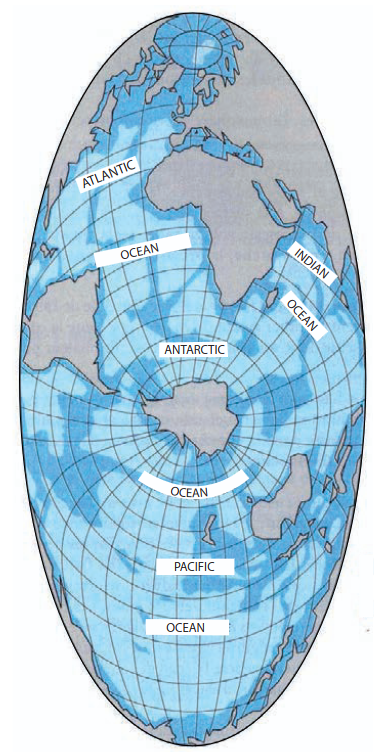
\includegraphics[width=0.3\linewidth]{images/01_intro/continuity_planteraryocean_fieux}
		\caption{Illustration de l'Océan Austral et de la connexion entre tous les océans (\cite{fieux_ocean_planetaire})}
		\label{fig:continuityplanteraryoceanfieux}
	\end{figure}
	
	Un \textbf{biotope} correspond à l'espace physique et les conditions abiotiques associées dans lesquelles vit une biocénose. Une \textbf{biocénose} est l'ensemble des populations d'organismes qui occupent une zone donnée et interagissent entre elles. L'océan étant un milieu continu, seuls la distance géographique et les paramètres physiques de l'eau (abiotiques) conditionnent la régionalisation en biotopes. La connaissance des paramètres physiques de l'eau est donc particulièrement importante pour l'étude des distribution des organismes et \textbf{niches écologiques} \footnote{\textbf{Niche écologique :} ensemble des conditions environnementales permettant à une espèce de survivre et de se reproduire \cite{hutchinson1957}.} marines. 
	
	\vspace{0.5em}
	
	Les principaux \textbf{paramètres abiotiques} structurant les écosystèmes sont : les propriétés hydrologiques et hydrodynamiques de l'eau, la pression et la lumière \cite{dipper2022}.Les \textbf{propriétés hydrologiques} (température, salinité, composition chimique) de l'eau dépendent du climat : la chaleur et le vent induisent une évaporation rendant l'eau de mer plus salée, les précipitations induisent un adoucissement de la salinité. La composition chimique de l'eau de mer est fortement dépendante des apports du littoral (fer, nitrates, etc). \textbf{L'hydrodynamisme} inclue les marées et les divers courants induits par des gradients de température, de pressions. Ces derniers dépendent majoritairement du vent et de l'ensoleillement.  \textbf{L'éclairement} (intensité et spectre) est  structuré verticalement selon la profondeur à cause des propriétés d'absorption de l'eau(Annexe \ref{annexe:strat_vert}, figure \ref{fig:stratverticalelmarineecology}). On parle de milieu eutrophe (épipélagique) entre 0 et 200m, de milieu dysphotique (mésopélagique) entre 200 et 1000m, de milieu aphotique (bathypélagique) entre 1000 et 4000m et de milieu abyssal au delà de cette dernière. La pression croit avec la profondeur et une stratification arbitraire est également appliquée selon cette variable (Annexe \ref{annexe:strat_vert}, figure \ref{fig:stratverticalelmarineecology}). La proximité au littoral participant grandement à la modification de ces paramètres abiotiques, on sépare arbitrairement l'océan horizontalement selon sa distance au plateau continental. On parle de \textbf{zone pélagique} au delà du plateau continental. Le contexte actuel de changement global induit des modifications importantes de l'expression de ces paramètres et induit en conséquence des changements de structuration des écosystèmes océaniques \cite{doney2012}, \cite{sallee2018}.
	
	\vspace{0.5em}
	
	\textbf{L'écologie} est une discipline qui s'intéresse aux interactions entre les différentes espèces d'un même biotope. Parmi elles, les\textbf{ relations trophiques} (alimentaires) jouent un rôle fondamentale dans la structuration des écosystèmes (figure \ref{fig:trophicnetworkelmarineecology}).
	
	\begin{figure}[H]
		\centering
		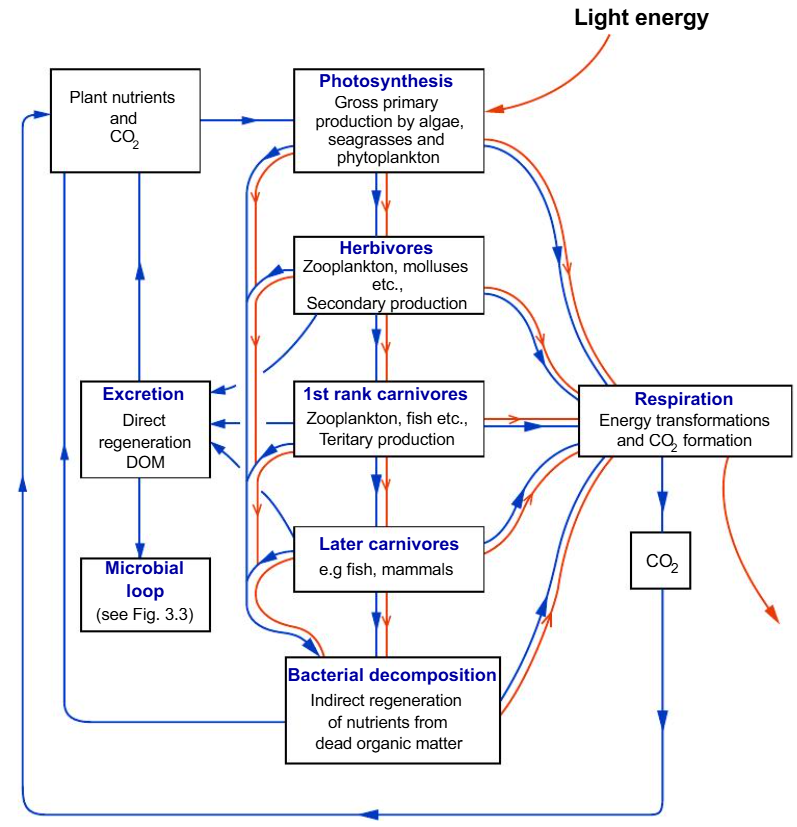
\includegraphics[width=0.7\textwidth]{images/01_intro/trophic_network_el_marine_ecology}
		\caption{Schéma du réseau trophique océanique \cite{dipper2022}.}
		\label{fig:trophicnetworkelmarineecology}
	\end{figure}
	
	Les \textbf{producteurs primaires} supportent tout le réseau trophique. Leur capacité à transformer la matière inorganique en matière organique (organismes autotrophes) les positionnent à la base du réseau. En effet, de nombreux organismes (hétérotrophes) n'ont pas cette capacité et dépendent uniquement des apports organiques de leur alimentation pour survivre. Le producteur primaire du milieu pélagique est le \textbf{phytoplancton}. Ce terme désigne tous les organismes végétaux (\textit{"phyto"}) n'ayant pas la capacité de se déplacer contre le courant (\textit{"plancton"}). Ce sont des organismes \textbf{photo-autotrophes}, c'est-à-dire, qu'ils peuvent soutenir leur métabolisme uniquement grâce à l'énergie lumineuse. Le processus bio-chimique permettant la transformation de l'énergie lumineuse en énergie chimique utilisable par le métabolisme est la \textbf{photosynthèse}. Ce processus nécessite la présence de \textbf{pigments photosynthétiques} chez les organismes l'effectuant. 
	Les \textbf{consommateurs primaires} sont les organismes s'alimentant des producteurs primaires. Dans le contexte du milieu pélagique, c'est le \textbf{zooplancton} \footnote{\textit{"Zoo"} : animal, \textit{"Plancton"} : n'ayant pas la possibilité de se déplacer à contre-courant.} et le \textbf{micronecton} \footnote{Petits poissons pélagiques.}. 
	Les\textbf{ niveaux trophiques intermédiaires} sont tous les étages de la chaine alimentaire, correspondent à tous les organismes situés entre les producteurs primaires et les prédateur supérieurs (dernier niveau du réseau trophique).
	
	
	\section{Secteur Indien de l'Océan Austral}
	L'océan Austral (ou Antarctique) forme un anneau autour de l'Antarctide. Il représente 22\% de la surface totale des océans. Contrairement aux autres océans, il n'est pas délimité par des frontières continentales. En regardant une carte (voir figure \ref{fig:continuityplanteraryoceanfieux}), on pourrait penser qu'il est simplement la prolongation du bassin Atlantique, Pacifique et Indien. En réalité, il est délimité par une frontière océanographique : le Front Subtropical (approximativement à 40°S), caractérisé par de très forts gradients de températures(figure \ref{fig:currentsfieuxroi}). L'océan Austral se distingue également des autres océans par l'uniformité de son climat, de son hydrodynamisme et de ses propriétés hydrologiques. 
	\begin{figure}
		\centering
		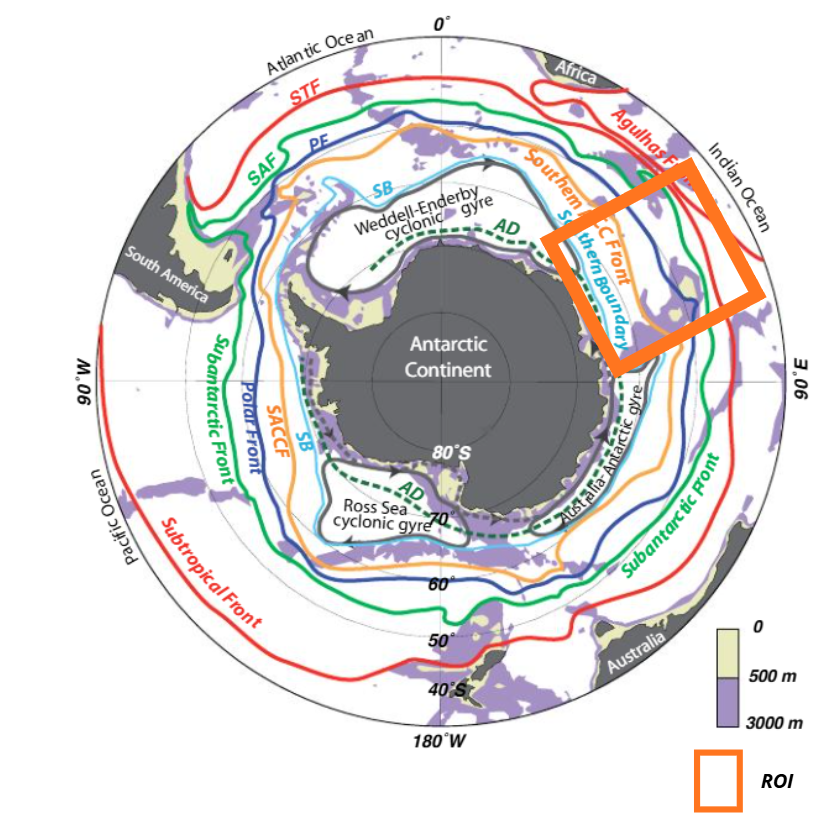
\includegraphics[width=0.5\textwidth]{images/01_intro/currents_fieux_ROI}
		\caption{Positions moyennes du Front subtropical (STF), du Front subantarctique (SAF), du Front sud du Courant circumpolaire antarctique (SACCF), de la Divergence antarctique (AD), ainsi que des trois gyres cycloniques du bassin de Weddell-Enderby, du bassin Antarctique-Australien et de la mer de Ross \cite{fieux_ocean_planetaire}.}
		\label{fig:currentsfieuxroi}
	\end{figure}
	
	\textbf{parler du sous échantillonage de la région, de sa vasteté et de son importance dans le carbon uptake etc}
	
	\subsection{Contexte physico-chimique de la région}
	Le secteur indien de l'Océan Austral est situé entre 20° et 80°E de longitude et s'étend de 30° à 70°S de latitude (figure \ref{fig:currentsfieuxroi}, \ref{fig:indiansectorsolatshiftpolarfronts}). Dans notre étude, la région d'intérêt (ROI) correspond au secteur Indien restreint en longitude (45-90°E, 30-60°S). Cette zone est caractérisée par plusieurs éléments : un fort gradient latitudinal de température, des changements bathymétriques importants (plateau de Crozet et Kerguelen) et un fort hydrodynamisme (Courant des Agulhas, front subtropical, front subantarctique, front polaire) (voir figure \ref{fig:indiansectorsolatshiftpolarfronts}). 
	
	\textbf{parler du faible eclairement, des concentrations en fer nitrates etc limitante, de la couverture de glace et de l'apport en fer de kerguelen}
	\begin{figure}[H]
		\centering
		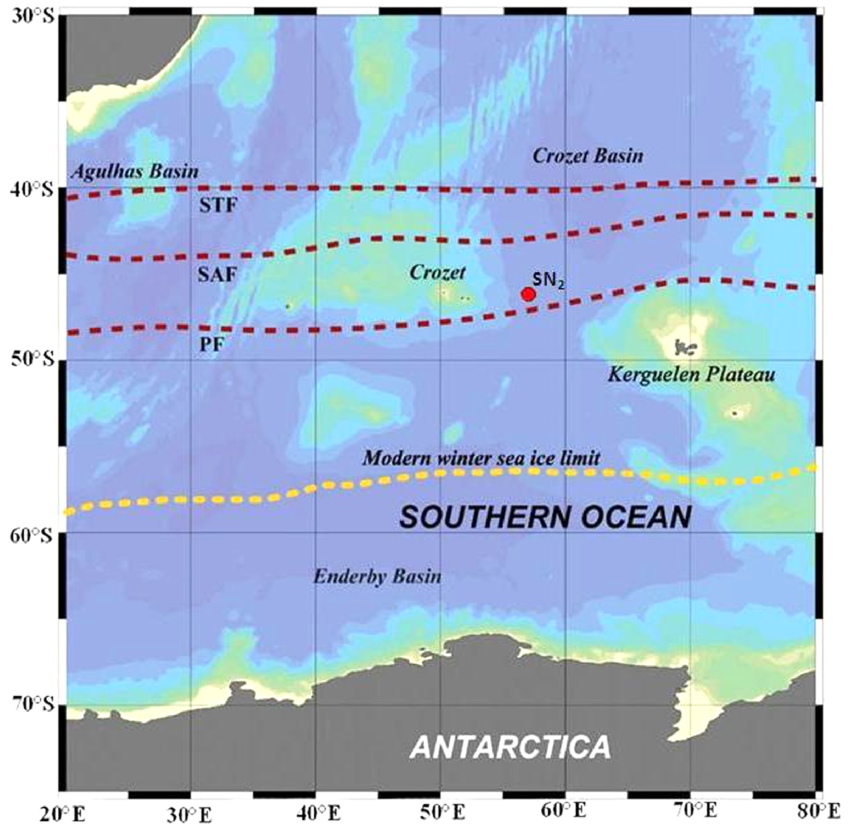
\includegraphics[width=0.5\textwidth]{images/01_intro/indian_sector_SO_lat_shift_polar_fronts}
		\caption{Carte du secteur Indien de l'Océan Austral et des courants \cite{shetye2013}}
		\label{fig:indiansectorsolatshiftpolarfronts}
	\end{figure}
	
	\subsection{Contexte biologique}
	D'un point de vue écologique, le réseau trophique de la région contient peu de niveaux. Le producteur primaire du milieu pélagique est le phytoplancton. Les communautés phytoplanctoniques \footnote{Composition taxonomique en phytoplancton du milieu} sont structurées selon un axe latitudinal. \textbf{recherches sur les structures phytoplanctoniques de base}
	Les consommateurs primaires sont le zooplancton et le micronecton. Plus particulièrement, la région est marquée par une forte abondance de Krill et d'euphosiacés.
	\textbf{parler des communautés phyto observées (pcq plus tard on présentera les chgms) la forte productivité primaire de la région et de la forte saisonnalité}
	
	Les prédateurs supérieurs sont les éléphants de mer, manchots,..
	\subsection{Et dans un contexte de changement climatique ?}
	Dans un contexte de changement global, les caractéristiques physico-chimiques de l'eau et de l'atmosphère changent également. Des études récentes ont annoncé par exemple des changements de régime de vent , une diminution de la profondeur de la couche de mélange \footnote{text}, une altération des courants de circulation, une migration au sud du front polaire, un réchauffement de la température de surface, un changement du flux du fer et des changements dans la proportion de couverture de la glace induisant une diminution de la salinité de l'eau (adoucissement). \cite{sallee2018}, 
	
	Ces changements affectent les organismes habitant ces milieux, comme le phytoplancton. Des études récentes font l'hypothèse d'une augmentation de la production primaire totale et d'une restructuration des communautés phytoplanctonique (\cite{adroli2026} : la contribution relative des diatomées dans la production primaire diminuerait. Au contraire, la contribution relative des haptophytes et des cryptophytes (nano/picophytoplankton ?) \cite{hayward2024Antarctic}
	
	+ des changements de temporalité des blooms et de leur durée et amplitude(être + précise dans quel sens) \cite{thomalla2023Widespread}
	
	\footnote{"In marine climate systems, a regime shift refers to a persistent reorganisation of physical and ecological system structure, variability and feedback processes thatt results in a transition toward a new dominant state rather than a short term interannual fluctuation \cite{abram2025Antarctic}}
	
	\textbf{développer les observations de ces changements et les hypothèses + long terme }
	
	\textbf{développer les hypothèes sur les effets sur les NTI(trophic cascade)}
	changements de temoralité/durée/amplitude des blooms => dictate the amount of biomass being generated within a season that can be exported to the ocean's interior or transferred to higher trophic levels \cite{thomalla2023Widespread}
	
	\section{Question scientifique}
	Ce projet de recherche s'intéresse à l'influence du type phytoplanctonique sur les niveaux trophiques intermédiaires du secteur Indien de l'Océan Austral
	
	\section{il manque}
	\textbf{RESTREINDRE LES HYPOTHESES A L'ETE et a la ROI si possible}
	la présence de l'importance de l'atmosphere dans les params physicochimique (vent mixing water, increase in CO2,more clouds = less light, etc)
	l'importance du so dans le contexte de changement global (carbon uptake, ..)
	reseau trophique + dtaillé du so
	Le changement climatique dans l'ocean austral
	phytoplancton du so : enorme vers kerguelen, limité par lumière et iron 
	Les changements de commu phyto observés
	Les hypothèses de changements /les changements observés dans les niveaux trophiques supérieurs (etude avec le carbone, article de ziad) : ramifications trophodynamique (southern ocean in a changing climate, climate drivers of so phytoplankton community)
	hypothèses claires des changements physiques de la zone (changement de flux d'iron (avec sea ice zone differentes) , chgmt de régime de vent, stratification, chgmt de mld (decreased), stratification alteration des pattern de circulation, southward migration of ocean fronts, increas in sst, changes in sea ice cover)
	hypothèses claires des changements de commu phyto induits (augmentation chla totale diminution contribution des diatoms, auglntation de contribution des petits phyto)
	hypothèses claires des changements de nti induits (ramification)
	
	
	
	
	
	
	
	
	
	
	
	
	
	
	
	
	\clearpage
	\chapter{Matériel}
	Les données séléctionnées pour notre étude servent de proxy aux paramètres abiotiques clés dans la régionalisation des écosystèmes (développés dans la section \ref{section:generalites}) et de proxy pour l'étude des organismes d'intéret (phytoplancton, niveaux trophiques intermédiaires).
	L'hydrodynamisme est approximé par le modèle de Finite-Time Lyapunov Exponent et les données hydrologiques sont approximées par les données de modèles du Copernicus Marine Service. La production primaire est déduite des concentrations depigments issues du modèle PIGMeANN. Enfin, la distribution des niveaux trophiques intermédiaires est approchée par acoustique active à 38 et 120kHz. 
	
	Ces quatres ensembles de données sont au moins tri-dimensionnels (temps, longitude, latitude). Une quatrième dimension (profondeur) est également présente pour les données d'acoustique active et de température/salinité.
	
	L'étude a été réalisée sur les années 2018, 2021, 2022 et 2023, en été afin de limiter la variabilité saisonnière, et de jour (calculé selon l'angle solaire), afin de limiter l'effet de la migration verticale journalière (DVM).
	
	\section{Concentrations de pigments photosynthétiques (PIGMeANN)}
	L'analyse de la couleur des océans à partir d'images satellite permet de d'étudier le phytoplancton sur une échelle spatiale et temporelle large. Historiquement les études se sont concentrées sur l'analyse de la chlorophylle-a de surface \cite{thomalla2023Widespread}. Plus récemment, des méthodes de deep learning on permis la caractérisation de "Phytoplankton Functional Types" et de "Phytoplakton Size Classes"  depuis des images satellites (par exemple Physat).  La radiance renvoyée par les océans a une couleur dépendant des pigments photosynthétiques qu'ils contiennent. L'idée est d'identifier une empreinte spectrale et de l'associer (deep learning) avec des mesures \textit{in-situ} High Performance Liquid Chromatography \footnote{L’échantillon est injecté dans une colonne traversée par un solvant sous haute pression, où ses différents composés sont séparés puis détectés individuellement. Permet de séparer et quantifier les pigments afin d’identifier les différents groupes présents.} et de cytométrie en flux\footnote{Les cellules sont entraînées individuellement devant un laser qui mesure leur diffusion (taille/forme des cellules) et leur fluorescence. On peut ensuite identifier les taxons.} qui caractérisent la présence et la structure des communauté phytoplanctoniques. 
\begin{table}[H]
	\centering
	\renewcommand{\arraystretch}{1.3}
	\begin{tabular}{
			>{\raggedright\arraybackslash}p{3.4cm}
			>{\raggedright\arraybackslash}p{2.0cm}
			>{\raggedright\arraybackslash}p{4.8cm}
			>{\raggedright\arraybackslash}p{2.6cm}
		}
		\hline
		\textbf{Pigment} & \textbf{Abréviation} & \textbf{Groupe phytoplanctonique associé (PFD)} & \textbf{Classe de taille} \\
		\hline
		Divinyl chlorophylle $a$ & dvChla & Procaryotes picoplanctoniques (\textit{Prochlorococcus}) & Picophytoplancton \\
		Chlorophylle $a$ & Chla & Marqueur de biomasse totale (tous groupes) & -- \\
		Chlorophylle $b$ & Chlb & Chlorophycées / Prasinophycées & Picophytoplancton \\
		Zéaxanthine & Zea & Cyanobactéries (\textit{Synechococcus}) & Picophytoplancton \\
		Fucoxanthine & Fuco & Diatomées (dominantes) & Microphytoplancton \\
		19'-hexanoyloxyfucoxanthine & Hex & Prymnésiophycées (haptophytes) & Nanophytoplancton \\
		19'-butanoyloxyfucoxanthine & But & Prymnésiophycées / pélagophytes & Nanophytoplancton \\
		Alloxanthine & Allo & Cryptophycées & Nanophytoplancton \\
		Péridinine & Per & Dinoflagellés (péridiniens) & Microphytoplancton \\
		\hline
	\end{tabular}
	\renewcommand{\arraystretch}{1}
	\caption{Pigments photosynthétiques analysés et groupes phytoplanctoniques associés (PFD) dans le secteur de Kerguelen en été/printemps austral, d'après Lasbleiz et al. (2014).}
	\label{tab:pigments}
\end{table}
	
	Sari El Dine a récemment mis en place la méthode de deep-learning PIGMeANN \cite{sari2026regional} permettant de distinguer des les concentrations de surfce de neuf pigments photosynthétiques(tableau \ref{tab:pigments}) sur l'ensemble de la couverture spatiale de l'image satellite donnée en entrée (exemple de prédiction avec la Chorophylle-a figure \ref{fig:mapchla2023-01-26}).  
	
	\begin{figure}[H]
		\centering
		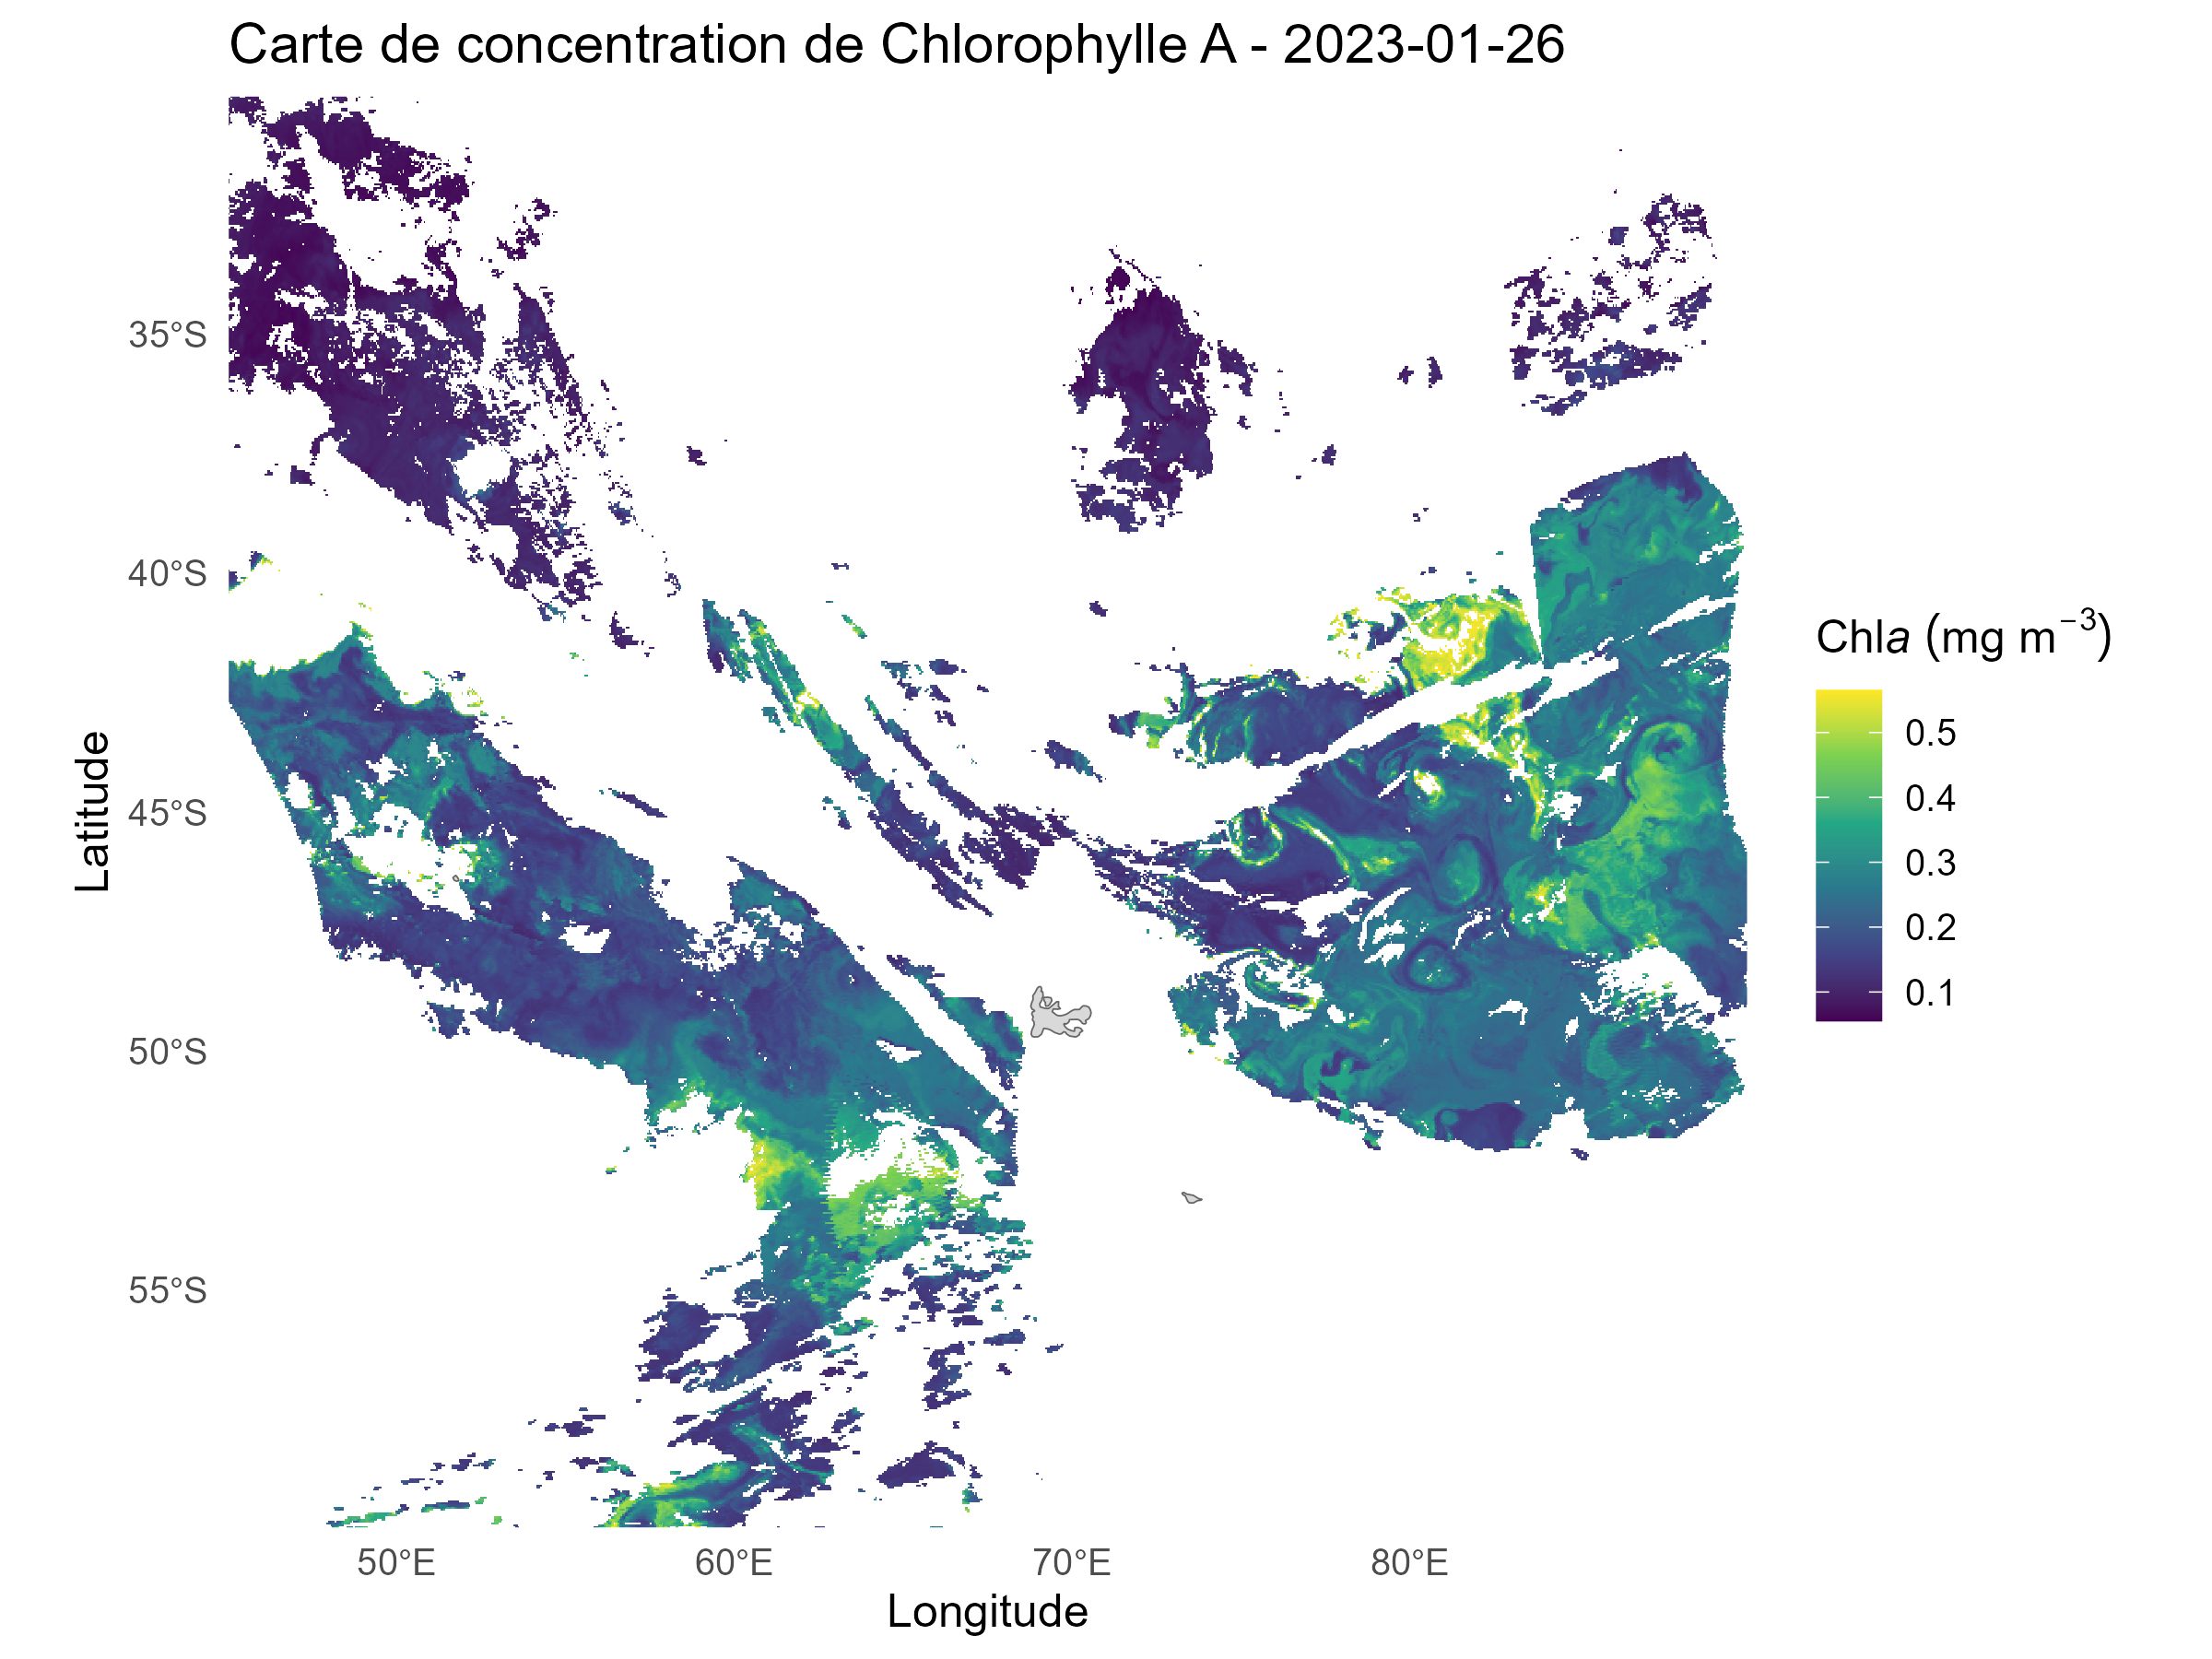
\includegraphics[width=0.8\textwidth]{images/02_materiel/map_chla_2023-01-26}
		\caption{Carte de prédiction de la concentration de Chlorophylle-a le 2023-01-26 sur le secteur indient du SO, prédictions issue de l'alorithme PIGMeANN développé par Sari el Dine \cite{sari2026regional}.}
		\label{fig:mapchla2023-01-26}
	\end{figure}
	
	A partir de la connaissance des différentes communautés phytoplanctoniques présente dans la région d'étude, et en s'appuyant notamment sur des études récentes \cite{sari2025influence}, \cite{heidemann2024drivers} \cite{Georges2014}, on peut relier certains pigments à des groupes phytoplanctoniques (PFD) ou Phytoplankton Size Classes (PSC). Ainsi on peut identifier la composition des communautés phytoplanctoniques à partir des différents assemblage de concentration de pigments prédites \ref{tab:pigments}. A noter que plusieurs taxons phytoplanctoniques peuvent partager les mêmes pigments photosynthétiques, ce pourquoi on identifie des PFD/PSC et non des taxons.
	
	Dans notre étude, les concentrations de pigments photo-synthétiques ne sont pas manipulées directement. On s'intéresse à la proportion de chaque pigment dans la quantité de pigments totale. Pour chaque pigment, on calcule donc son ratio sur la somme de tous les pigments\footnote{La Chlorophylle-a est exclue car peu informative : en effet, il est présent à de fortes concentration, la majorité des organismes possèdant ce pigment.}
	
	\section{Données hydrologiques de température et salinité (CMEMS)}
	Les données de températures et salinité sont issues de la plateforme Copernicus \footnote{Programme d’observation de la Terre de l’Union européenne, qui fournit notamment des données et services permettant de surveiller et comprendre l’état de l’environnement, dont l’océan \cite{copernicus2026services}}. Ce sont des données issues des observations temps-réelles CMEMS \footnote{Copernicus Marine Environment Monitoring Service, service marin de Copernicus} et réanalysées par le modèle NEMO \footnote{Nucleus for European Modelling of the Ocean, modèle numérique de l’océan qui simule l’évolution de paramètres comme la température, la salinité, les courants et le niveau de la mer}, et ERA5 \footnote{Modèle atmosphérique de l'ECMWF (European Centre for Medium-Range Weather Forecasts) qui fournit les conditions atmosphériques nécessaires pour forcer le modèle océanique NEMO à sa surface}.
	Sont téléchargées tous les profils de température ("thetao") et de salinité ("so") entre 45-90°E de longitude et 30 et 60°S de latitude, avec une résolution spatiale de 0,083° et une résolution temporelle journalière, sur les quatres années étudiées : 2018, 2021, 2022, 2023, entre janvier et mars. 
	
	\section{Données hydrodynamiques : Finite Time Lyapunov Exponent}
	Le Finite Time Lyapunov Exponent est un indicateur qui, à partir des données de champs de courants, permet de caractériser la séparation ou la convergence de trajectoires de particules d’eau sur une durée finie. On peut ainsi identifier les structures dynamiques susceptibles de contrôler le transport et la dispersion dans l’océan \cite{shadden2005definition}, \cite{dovidio2004mixing}.
	
	\vspace{0.5em}
	
	On considère un champ de vitesse bidimensionnel dépendant de la position et du temps, issu des données de réanalyse GLORYS21 de Copernicus Marine Service :
		\begin{equation}
			\mathbf{u}(x,y,t)
			=
			\begin{pmatrix}
				u(x,y,t)\\
				v(x,y,t)
			\end{pmatrix}
		\end{equation}
		avec $u$ et $v$ représentant respectivement les composantes zonale et méridienne de la vitesse, et où $\mathbf{x}=(x,y)$ désigne la position de la particule.
		
	À partir d'une position initiale $\mathbf{x}_0$ au temps $t_0$, la trajectoire d'une particule est obtenue en intégrant l'équation d'advection :
	
	\begin{equation}
		\frac{d\mathbf{x}}{dt}
		=
		\mathbf{u}(\mathbf{x},t),
		\qquad
		\mathbf{x}(t_0)=\mathbf{x}_0.
	\end{equation}
	
	Après une durée d'intégration $T$, la position finale de la particule peut être décrite à l'aide du flot lagrangien :
	
	\begin{equation}
		\mathbf{x}(t_0+T)
		=
		\mathbf{F}_{t_0}^{T}(\mathbf{x}_0),
	\end{equation}
	
	où $\mathbf{F}_{t_0}^{T}$ est l'application qui associe à chaque position initiale $\mathbf{x}_0$ sa position après une durée $T$.
	
	On peut ensuite analyser la variation des trajectoires $\mathbf{F}_{t_0}^T(x_0)$ après un temps $T$ si l'on change la position initiale $x_0$ des particules (tenseur de déformation): 
		\begin{equation}
			\nabla \mathbf{F}_{t_0}^{T}
			=
			\frac{\partial \mathbf{F}_{t_0}^{T}}{\partial \mathbf{x}_0}
			=
			\begin{pmatrix}
				\frac{\partial F_x}{\partial x_0} &
				\frac{\partial F_x}{\partial y_0} \\[6pt]
				\frac{\partial F_y}{\partial x_0} &
				\frac{\partial F_y}{\partial y_0}
			\end{pmatrix}
		\end{equation}
		
		Le tenseur de Cauchy-Green permet de quantifier la déformation des distances entre des particules initialement proches. Il est défini par :
		\begin{equation}
			\mathbf{C}_{t_0}^{T}(\mathbf{x}0)
			=
			\left(
			\nabla\mathbf{F}{t_0}^{T}(\mathbf{x}0)
			\right)^{T}
			\nabla\mathbf{F}{t_0}^{T}(\mathbf{x}_0).
		\end{equation}
		
		Le facteur maximal d'étirement entre les particules est donné par la plus grande valeur popre $\lambda_{max}$ du tenseur de Cauchy-Green $\mathbf{C}_{t_0}^{T} (\mathbf{x}_0)$
		
		Le FTLE ($\sigma_{t_0}^{T}$) est ensuite calculé, il correspond au taux de croissance logarithmique du facteur d'étirement maximal $\lambda_{max}$, normalisé par la durée d'intégration $T$ :
		
			\begin{equation}
				\sigma_{t_0}^{T}(\mathbf{x}_0)
				=
				\frac{1}{|T|}
				\ln\left(
				\sqrt{
					\lambda_{\max}\left(
					\mathbf{C}_{t_0}^{T}(\mathbf{x}_0)
					\right)
				}
				\right)
			\end{equation}
	
		avec :
		\begin{itemize}
			\item $\mathbf{C}_{t_0}^{T}$ le tenseur de Cauchy-Green, décrit comment les distances entre les particules évoluent. Il est calculé à partir des données de champs de courants
			\begin{equation}
				\mathbf{C}_{t_0}^{T}
				=
				\left(\nabla\mathbf{F}_{t_0}^{T}\right)^{T}
				\left(\nabla\mathbf{F}_{t_0}^{T}\right)
			\end{equation}
			\item $	\lambda_{\max}$ la plus grande valeur propre du tenseur de Cauchy-Green
			\item $\mathbf{x}_0$ la position initiale de la particule
			\item $T$ le tempsd d'intégration pendant lequel on suit la particule
			\item $\sigma$ le FTLE qui mesure le taux moyen de séparation des trajectoires des particules, exprimé en unité inverse du temps
		\end{itemize}
	
		\begin{figure}[H]
			\centering
			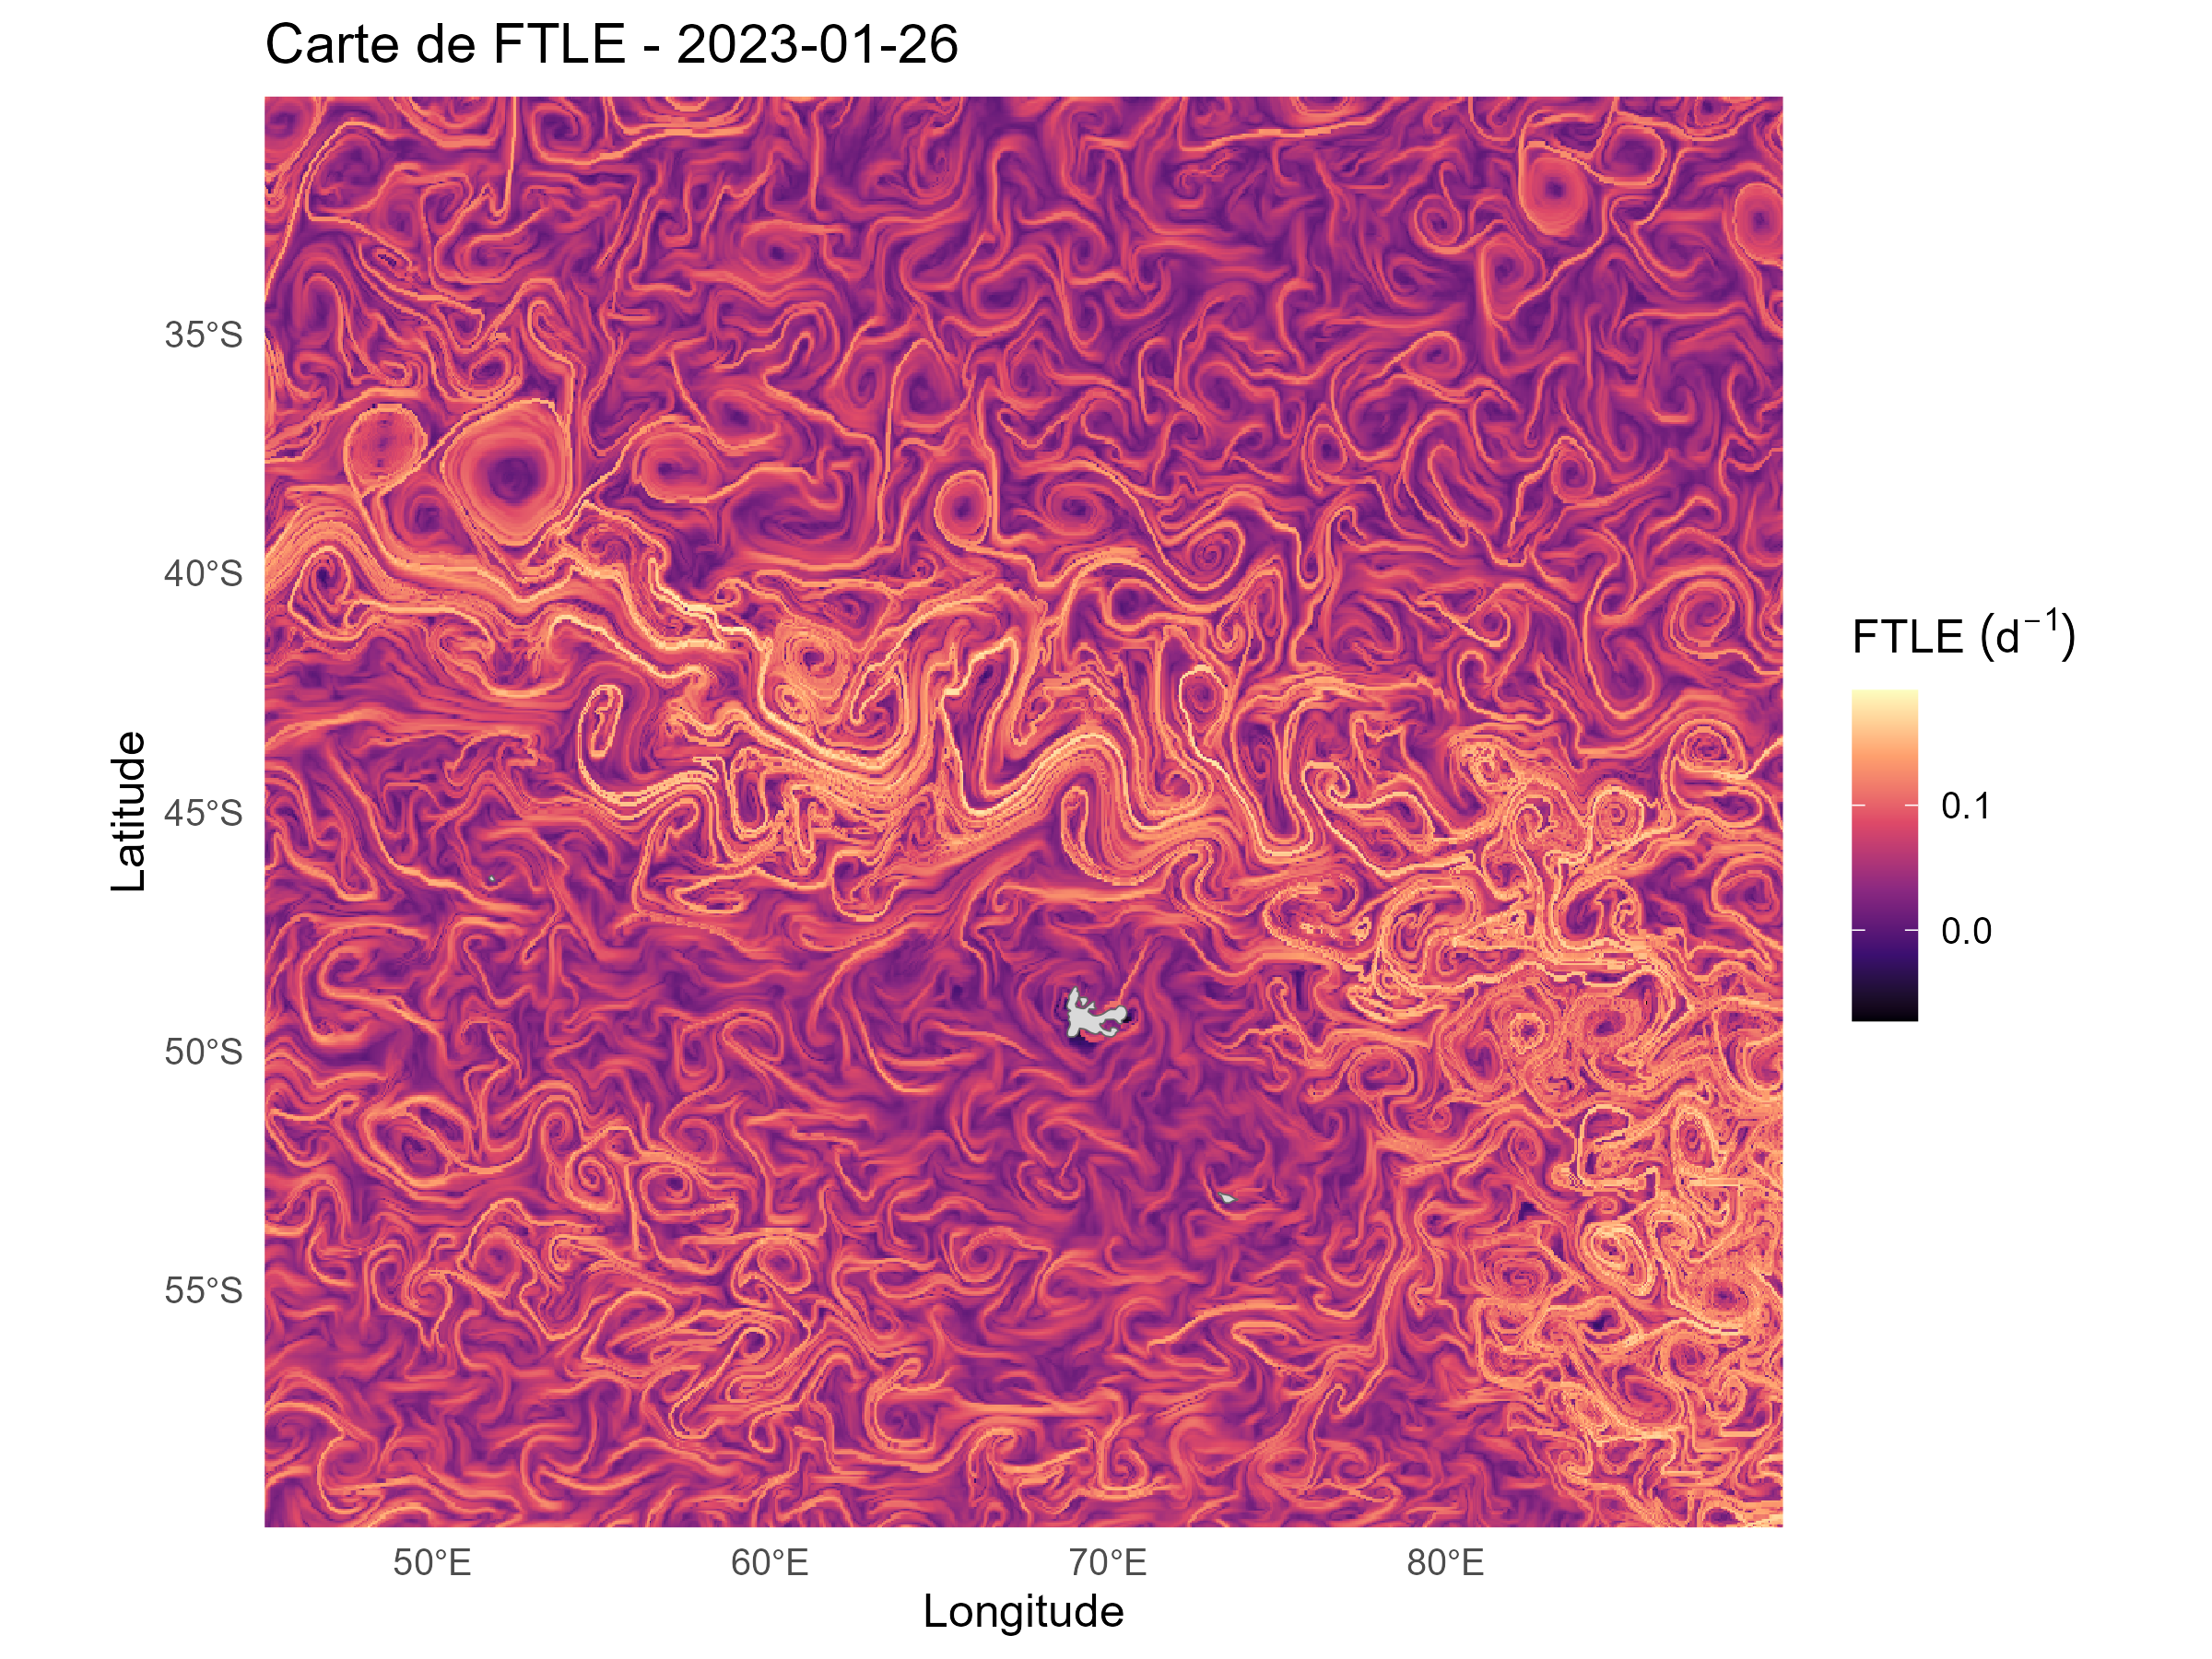
\includegraphics[width=0.7\textwidth]{images/02_materiel/map_ftle_2023-01-26}
			\caption{Advection Lagrangienne FTLE backward (90j) du 2023-01-26}
			\label{fig:mapftle2023-01-26}
		\end{figure}
	
	Dans notre étude, la durée d'advection est de quatre-vingt dix jours en backward. On obtient des cartes de FTLE $\in \mathbb{R}^{time \times lon \times lat}$ pour les années 2018, 2021, 2022, 2023 entre janvier et mars. La résolution temporelle est journalière et la résolution spatiale est de 0.05°.
	
	Une valeur élevée du FTLE indique une forte séparation des trajectoires voisines sur la période considérée. Les structures organisées apparaissant comme des crêtes de FTLE (voir figure \ref{fig:mapftle2023-01-26}) peuvent ainsi être utilisées pour identifier des frontières de transport ou des structures cohérentes lagrangiennes (Lagrangian Coherent Structures, LCS) dans l'écoulement \cite{shadden2005definition}. 
	
	
	
	\section{Données d'acoustique active (OBSAUSTRAL)}
	Les écosystèmes pélagiques sont difficilement observable. L'acoustique active est une méthode   consistant à émettre une onde, la réceptionner et analyser le signal reçu (principe du sonar) \cite{benoitbird2016ecological}. L'echo reçu résulte de la réflection du son émis par un objet (par exemple le fond marin (bathymétrie)), un organisme où encore des discontinuité physiques dans la colonne d'eau (i.e. changements de densité). Avec la connaissance de la vitesse locale de propagation du son dans l'eau, le délai avec lequel le signal est reçu et son intensité peuvent informer : la distance des backscaterrers (leur position dans la colonne d'eau), leur abondance, la composition taxonomique des organismes présents, voir également leur taille. Cette méthode à l'avantage de permettre un échantillonage de la colonne d'eau avec une résolution et couverture spatiale et temporelle importante. Elle est également non-invasive et non-exctractive.
	
	\begin{figure}[H]
		\centering
		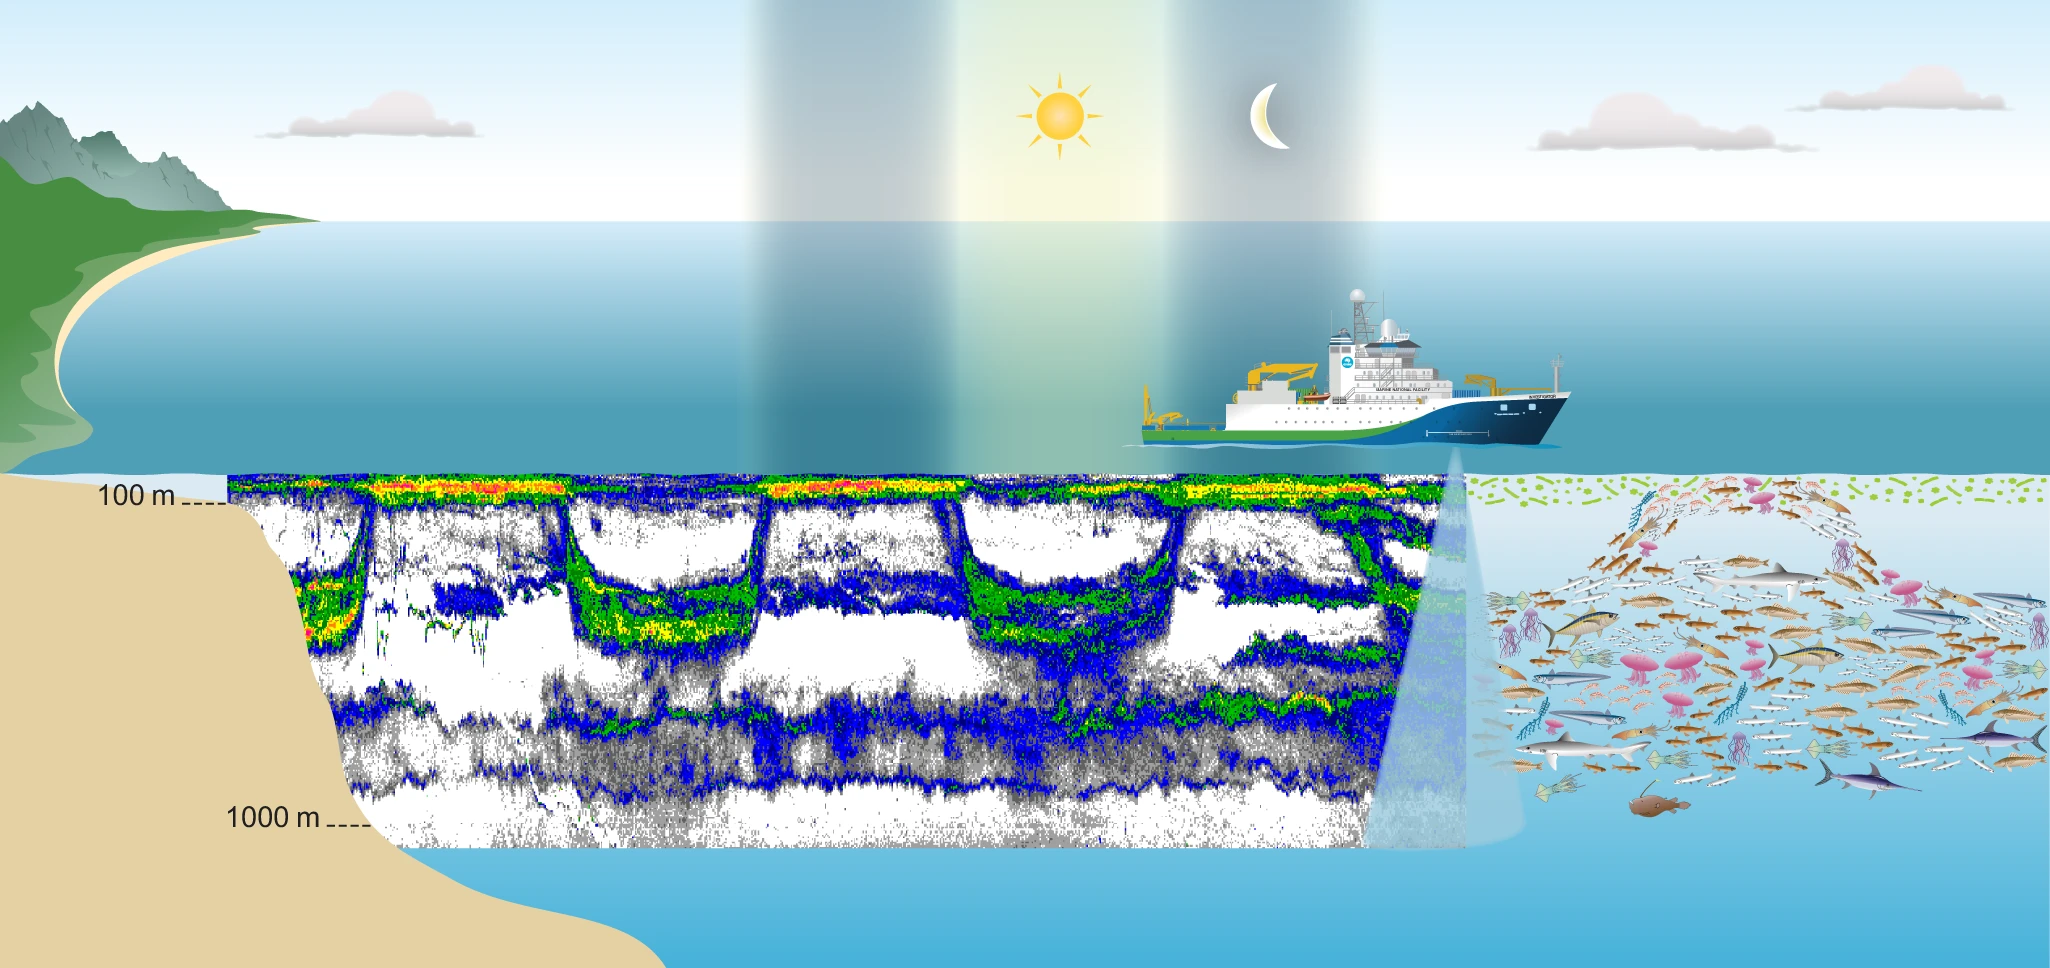
\includegraphics[width=\textwidth]{images/02_materiel/OBSAUSTRAL_acoustic_data_schema}
		\caption{Schéma explicatif illustrant l’acquisition de données d’acoustique active par des navires, permettant de caractériser la distribution des organismes dans la colonne d’eau à partir des signaux acoustiques enregistrés et représentés sous forme d’échogramme \cite{haris2021sounding}.}
		\label{fig:obsaustralacousticdataschema}
	\end{figure}
	
	La réfléctance des ondes acoustiques sur un objet dépend également de la fréquence émise. D'autre part, différents organismes ont des réponses fréquentielles différentes (voir Annexe \ref{annexe:rep_freq}, figure \ref{fig:freqresponse}). La méthode d'acoustique active ayant été développée par les pêcheries, la fréquence d'échosondeur de référence est 38kHz (fréquence à laquelle sont les poissons résonnent). 
	
	\vspace{1cm}
	
	Pour notre étude, nous avons utilisé des données d'acoustiques actives collectées en transect \footnote{Le bateau se déplace et collecte en même temps des données, ()par opposition aux données "stations" collectées lorsque le bateau est en arrêt). Celà a un coût en terme de résolution des spectrogramme et d'interprétabilité mais permet d'obtenir une plus grande couverture spatiale.} lors des campagnes océanographiques OBSAUSTRAL/THEMISTO \cite{flotteoceanographique_campagnes} lors des étés 2018, 2021, 2022, 2023.  Deux fréquences d'émissions ont été choisies pour notre étude : 38kHz (afin de comparer nos résultats avec la littérature) et 120kHz qui correspond à la fréquence à laquelle les Euphausiacés (krill) et Copépodes sont le plus détectable (voir Annexe \ref{annexe:rep_freq}, figure \ref{fig:freqresponse}). En effet, ces organismes sont en forte abondance et constituent des éléments importants du réseau trophiques de la région d'étude.
	
	
	\clearpage
	\chapter{Méthode}
	\section{Pré-traitement des données}
	\subsection{Calcul du Nautical Area Scattering Coefficient (NASC) \cite{IRD_MATECHO_User_Manual}}
	L'\textbf{Intensité de l'echo (IE) }correspond au signal reçu par le transducteur lorsqu'une onde est émise dans la colonne d'eau puis réfléchis par un objet.
	\begin{equation}
		IE = IS - 2TL + DI + TS
	\end{equation}	
	où 
	\begin{itemize}
		\item IS est l'intensité du son émise (dB) $IS = 10 \times \log_{10}(I/I_{ref}) $ et $I_{ref} = \rho_{ref}^{2} = 1 \mu \text{Pa}$ ($\rho_{ref}$ la pression de référence)
		\item TL la perte de transmission  \footnote{Le premier terme correspond à l'attenuation due à la dispersion de l'onde et le second terme correspondant à l'éttenuation de la propagation du milieu ($\alpha$ le coefficient d'absorption en $dB.m^{-1}$)} $TL = 20 \log_{10} (R) + \alpha R$
		\item DI : l'indice de directivité du transducteur (dB)
		\item TS la réfléctivité de la source (Target Strength) \footnote{$TS = 10 \log_{10}(P-r)+ 40 10 \log_{10}(R) + 2 \alpha R - 10 \log_{10}(\frac{P_t \lambda^{2}}{16 \pi^{2}} - 2 G_0)$ avec \begin{itemize}
				\item $P_r$ : puissance du signal reçu, mesurée aux bornes du transducteur (W).
				
				\item $P_t$ : puissance du signal transmis, référencée aux bornes du transducteur (W).
				
				\item $R$ : distance entre le transducteur et la cible détectée (m).
				
				\item $c$ : célérité du son dans le milieu (m/s).
				
				\item $\alpha$ : coefficient d'absorption du milieu (dB/m).
				
				\item $\lambda$ : longueur d'onde (m).
				
				\item $G_0$ : gain du transducteur sur l'axe acoustique, mesuré lors de la calibration du sondeur (dB).
		\end{itemize}}
	
		\vspace{1cm}
		
		Sur une échelle linéaire, le TS correspond à la \textbf{section efficace de rétrodiffusion} \(\sigma_{bs} = 10^{\frac{TS}{10}}\) (\(\mathrm{m^2}\)). Elle caractérise la capacité de la cible à rétrodiffuser l'énergie acoustique et est déterminée par référence à la section efficace de rétrodiffusion théorique de la sphère de calibration utilisée lors de la calibration du sondeur.
		
		\vspace{1cm}
		
		Le \textbf{volume backscattering coefficient} $s_v$ (en $m^{2}.m^{-3}$ ou $m^{-1}$) est la somme  toutes les surfaces réfléctives $\sigma_{bs}$ de toutes les cibles acoustiques dans le volume d'échantillonage V, normalisées à 1$m^{3}$.  Il mesure de la densité acoustique des organismes présents dans un volume d'eau. Un niveau de $S_v$ élevé correspond à une quantité plus importante de rétrodiffusion acoustique dans le volume échantillonné. Ce qui est interprété comme un nombre important d'organismes présents dans la colonne d'eau ou un organisme de taille importante ou encore un organisme ayant des propriétés réfléctives diffusantes \footnote{Beaucoup de poissons pélagiques ont des vessies natatoires, ce sont des organes leur permettant d'ajuster leur flottabilité. Cette vessie natatoire est connue pour particulièrement diffuser à 38kHz et donc augmenter artificiellement le volume de rétrodiffusion mesuré}.
		\begin{equation}
			s_v = \sum \sigma_{bs}/V
		\end{equation}
	\end{itemize}
	
	Le \textbf{Nautical Area Scattering Coefficient (NASC)}, noté $s_A$, correspond au coefficient de rétrodiffusion acoustique par unité de surface nautique (en $m^{2}.nmi^{-2}$) correspond à l'intégration sur l'ensemble de la colonne d'eau du volume backscattering coefficient en échelle linéaire $s_v = 10^{\frac {S_v} {10}}$ multiplié par un certain facteur (convention). Le NASC résume la rétrodiffusion acoustique sur une couche d'eau donnée.
	\begin{equation}
		s_A = 4 \pi (1852)^{2} \int_{z_{1}}^{z_{2}} s_v
	\end{equation}
	
	Pour notre étude, nous avons utilisé le NASC comme mesure approximant la biomasse de zooplancton et micronecton (NTI) présents dans la colonne d'eau. Les calculs de volume backscattering coeficient $s_v$ à partir de l'intensité de l'echo (IE) Isabelle Durand, ingénieure au MNHN. Pour les calculs du NASC, la profondeur d'intégration $z_1$ a été fixé à 25m pour limiter le biais d'échantillonage \footnote{effet de "bullage" du bateau bruitant les données à des faibles profondeurs}. Le choix de $z_2$ dépend de la fréquence de l'échosondeur : pour des fréquences de 38kHz et 120m, la colonne d'eau est échantillonné respectivement jusqu'à une profondeur moyenne de 700m et 300m (voir Annexe \ref{annexe:missing_values}, figure \ref{fig:diagnabydepthperesu}). A partir de ces profondeurs, beaucoup de profils de volume de rétropropagation acoustiques ont des valeurs manquantes. Afin d'éviter d'intégrer les coefficients de rétrodiffusion acoustique sur des profondeurs variables, les profils avec plus de 50\% de valeurs manquantes ont été exclues du jeu de donées. Les valeurs manquantes résiduelles situées entre deux profondeurs connues ont été comblées par interpolation linéaire. Les valeurs manquantes résiduelles situées aux extrémité du profil sont comblées en prolongant le profil par la valeur la plus proche. 
	
	\vspace{1cm}
	
	Ainsi, pour chaque profil de volume de retropropagation acoustique (ESU), on calcule le NASC qui nous donne un scalaire, le résumé de la rétrodiffusion acoustique sur l'ensemble de la couche d'eau considérée ([25-700]m pour 38kHz et [25-300]m pour 120kHz) (figure \ref{fig:diagnasctimeperesu120khz2023}).
		
	\begin{figure}[H]
		\centering
		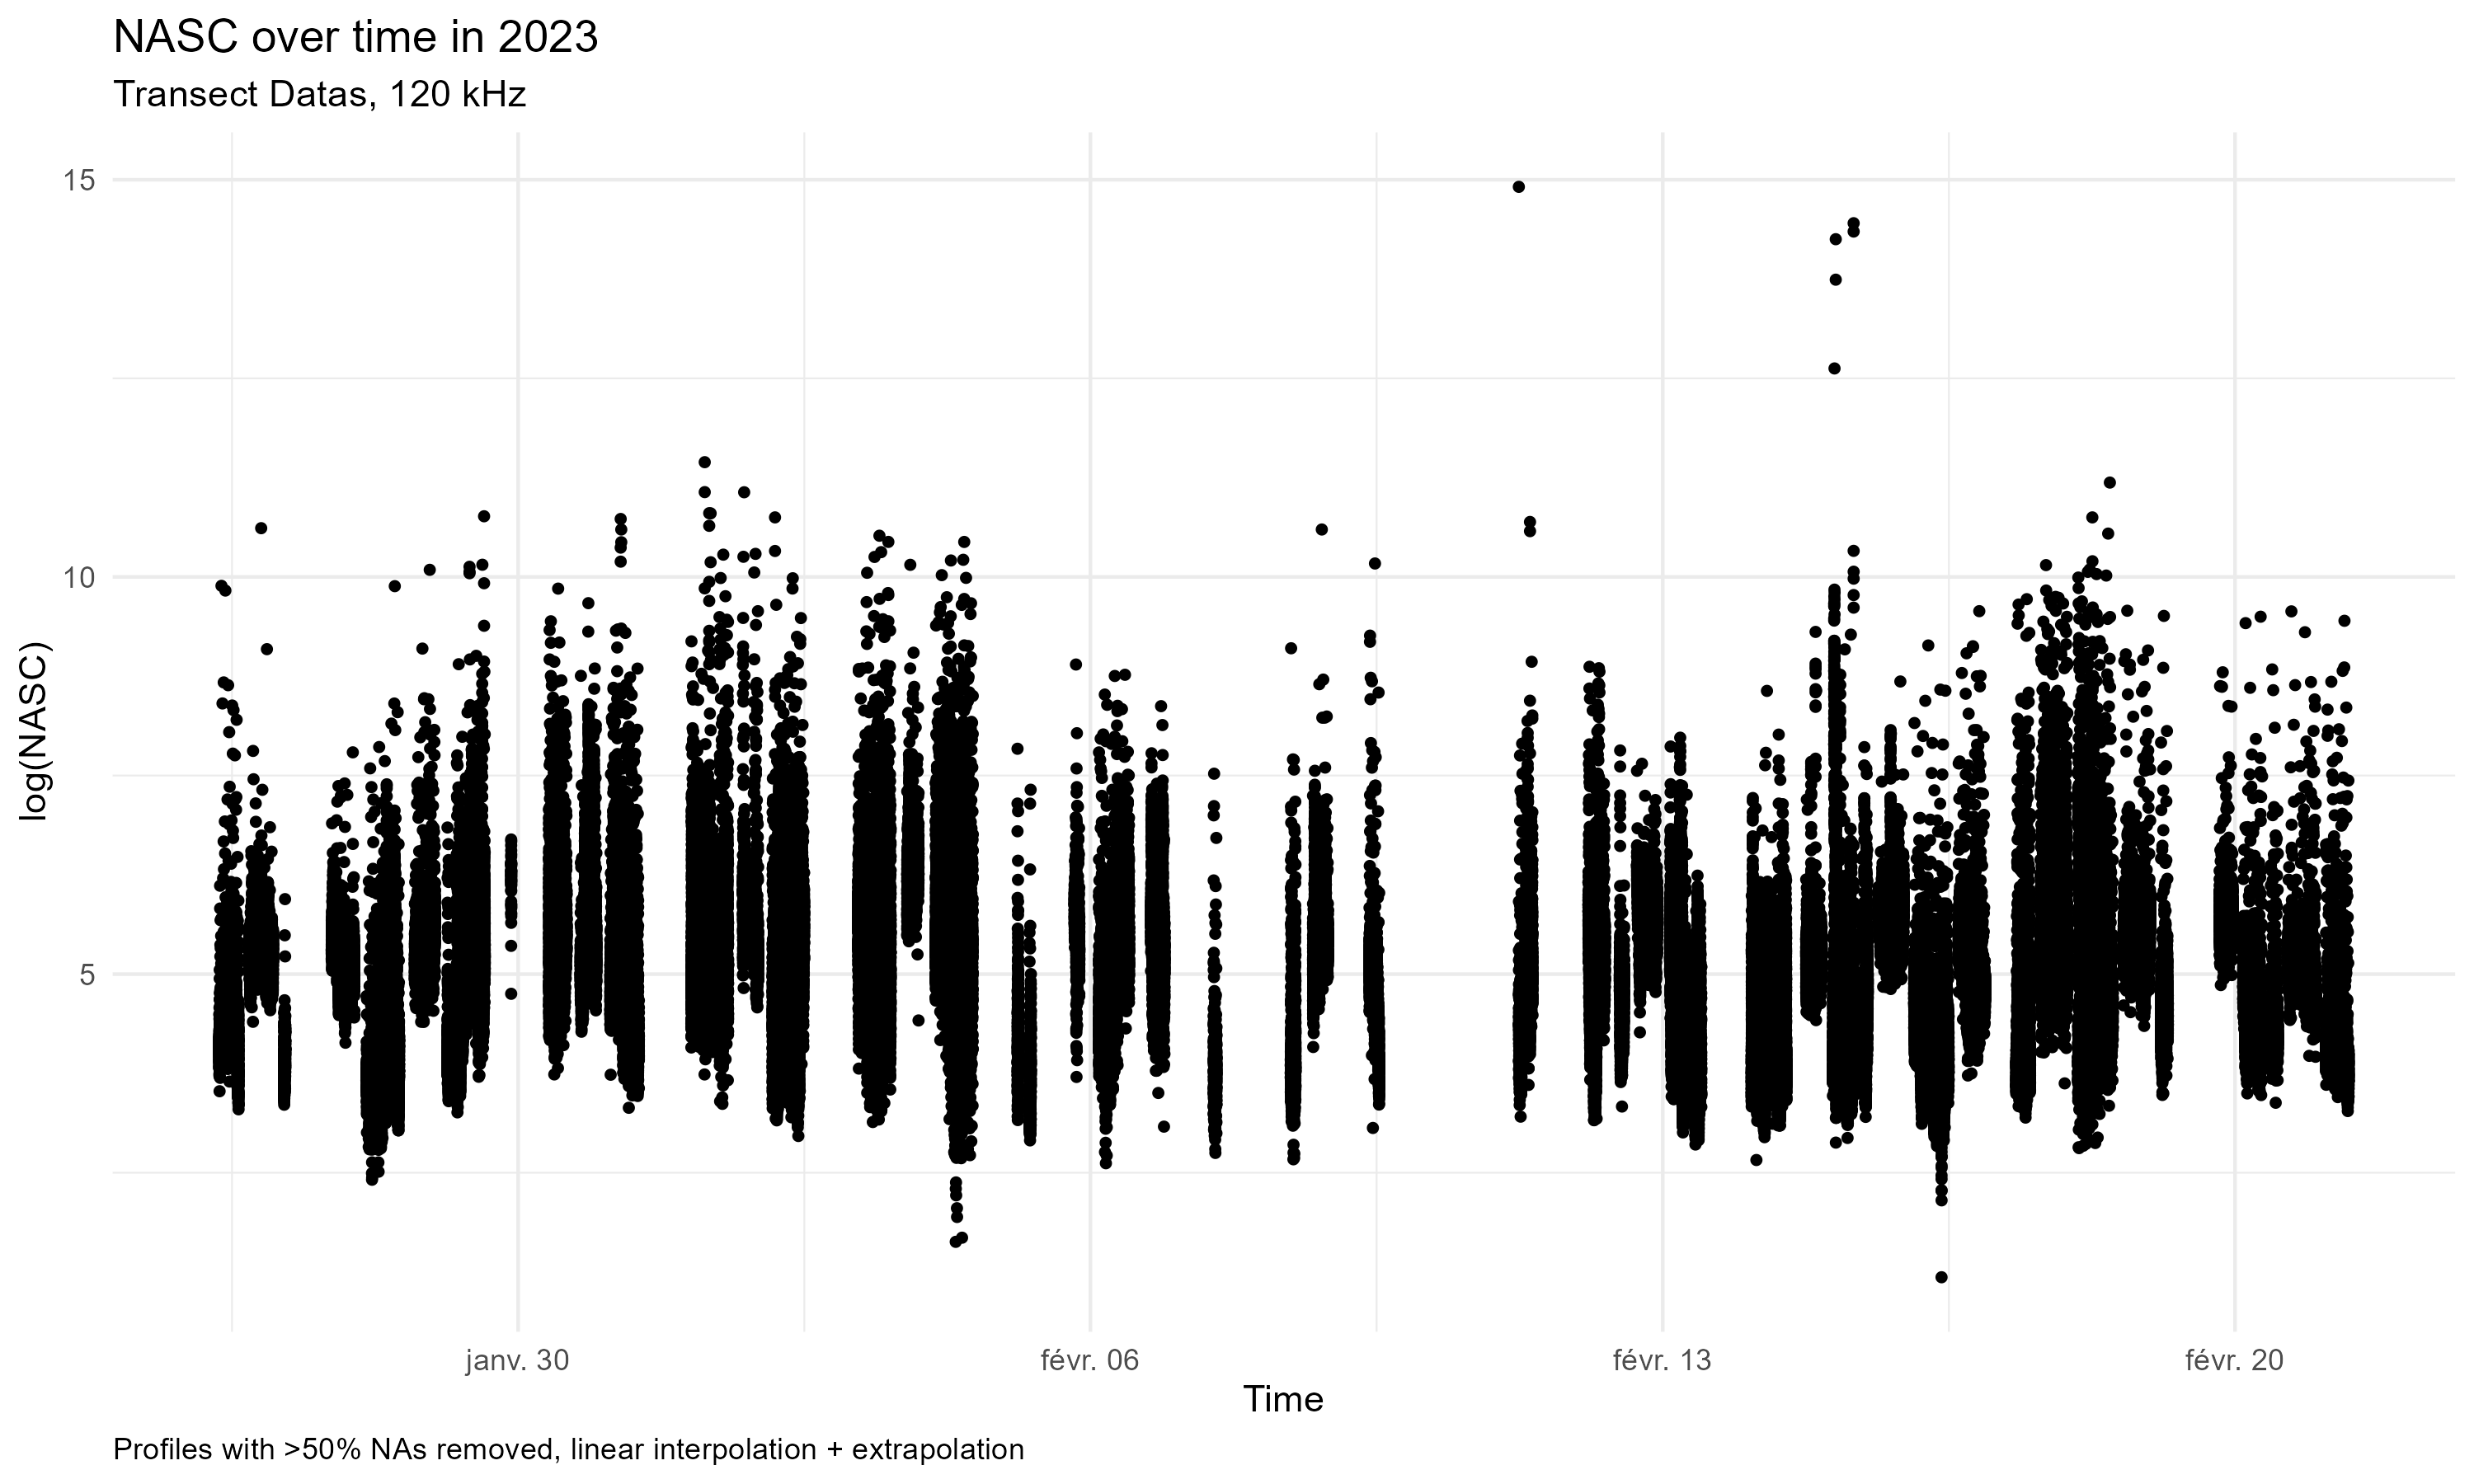
\includegraphics[width=\textwidth]{images/03_methodology/diag_NASC_time_per_esu_120kHz_2023}
		\caption{$log_{10}(NASC)$ en fonction du temps, données d'acoustique active (transect) issues de la campagne océanographique OBSAUSTRAL 2023 \cite{flotteoceanographique_campagnes}.}
		\label{fig:diagnasctimeperesu120khz2023}
	\end{figure}
	
	\subsection{Calcul des Functional Oceanographic Domain (FOD)}
	\subsubsection{Présentation des Domaines Océanographiques Fonctionnels}
	Les Domaines Océanographiques Fonctionels (ou Functional Oceanographic Domain) sont des masses d'eau ayant des caractéristiques thermohalines similaires. La méthode d'identification des FOD a été développé par Fonvieille N. et Nerini D. \cite{fonvieille2024}. Les données thermohalines (des modèles de Copernicus dans notre cas) sont, dans un premier temps (1), estimées dans un espace fonctionnel par projection sur une base de B-spline. Dans un second temps (2), la dimension de la matrice des coefficients de pondération des B-splines est réduite par une Analyse par Composante Principale (ACP ou PCA en anglais). Dans un dernier temps (3), un clusterning (GMM) est appliqué à $k$ composantes principales trouvé par la PCA. Ces trois étapes sont développées en Annexe \ref{annexe:methode_fod}.
	
	Dans notre étude, l'estimation fonctionelle par projection sur une base de B-splines a été effectué avec l'hyperparamètre de régularisation $\lambda = 0.25$ et pour $K=25$ B-splines. Sont convervées 6 composantes principales ($>0.99$ \% explained var., voir tableau \ref{tab:pca_variance}) pour le clustering. L'indice BIC nous permet de sélectionner $nclust = 6$ clusters. En ajoutant les classes de transitions, on obtient alors 13 clusters distincts (7 clusters de "transitions") \footnote{La classe "NA" correspond aux clusters manquants sur le plateau de Kerguelen. Les profils de température et salinité allant de 20 à 500m, sont retirés des calculs tout profils ayant des données manquantes entre ces deux valeurs. Les zones où la bathymétrie est inférieure à 500m sont donc exclues de ces calculs.} (voir figure \ref{fig:comparaisondofmap}). 
	
	\begin{figure}[H]
		\centering
		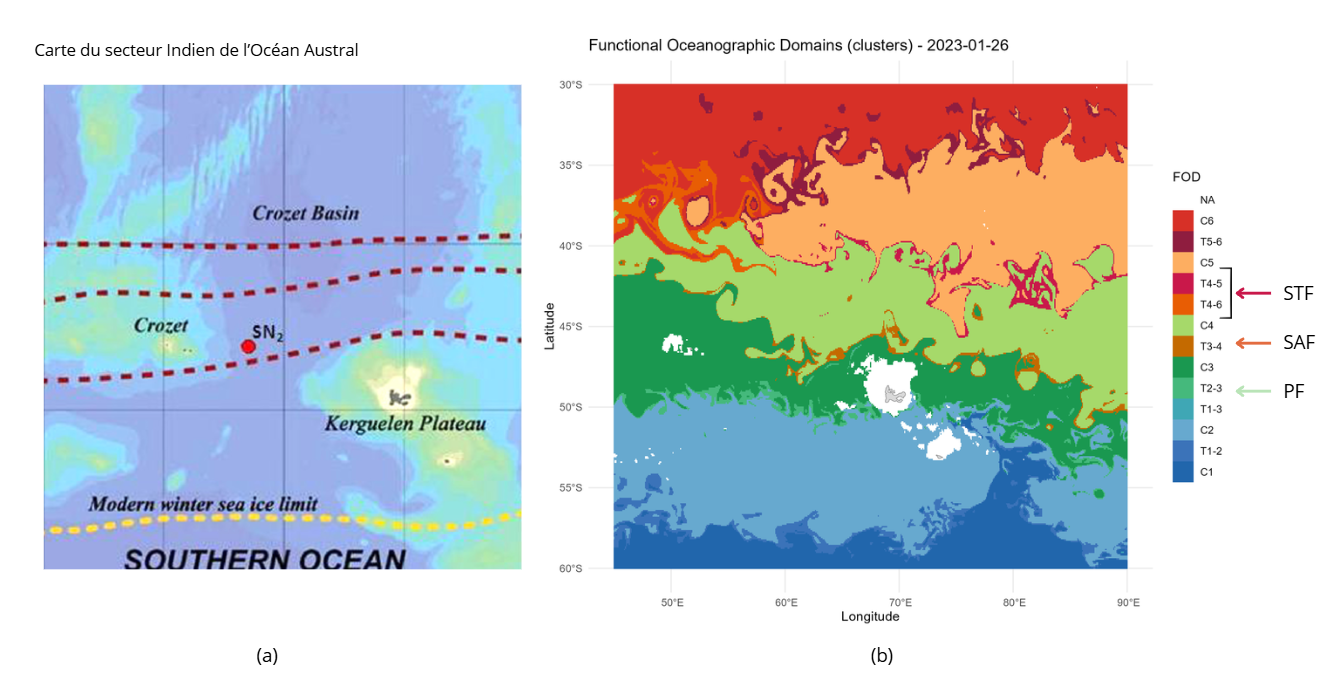
\includegraphics[width=\textwidth]{images/03_methodology/comparaison_dof_map}
		\caption{(a) Carte du secteur Indien de l'Océan Austral et des courants \cite{shetye2013} (b) Carte des Domaines Océanographiques Fonctionnels du 2023-01-26 générée par la méthode développée par Fonvieille N. et Nerini D. \cite{fonvieille2024}. Identification du Front Polaire (FP, cluster T2-3), du Front Subantarctique (SAF, cluster T3-4) et du Front Subtropical (STF, clusters T4-5 et T4-6)}
		\label{fig:comparaisondofmap}
	\end{figure}
	\begin{figure}[H]
		\centering
		\begin{subfigure}[b]{0.48\textwidth}
			\centering
			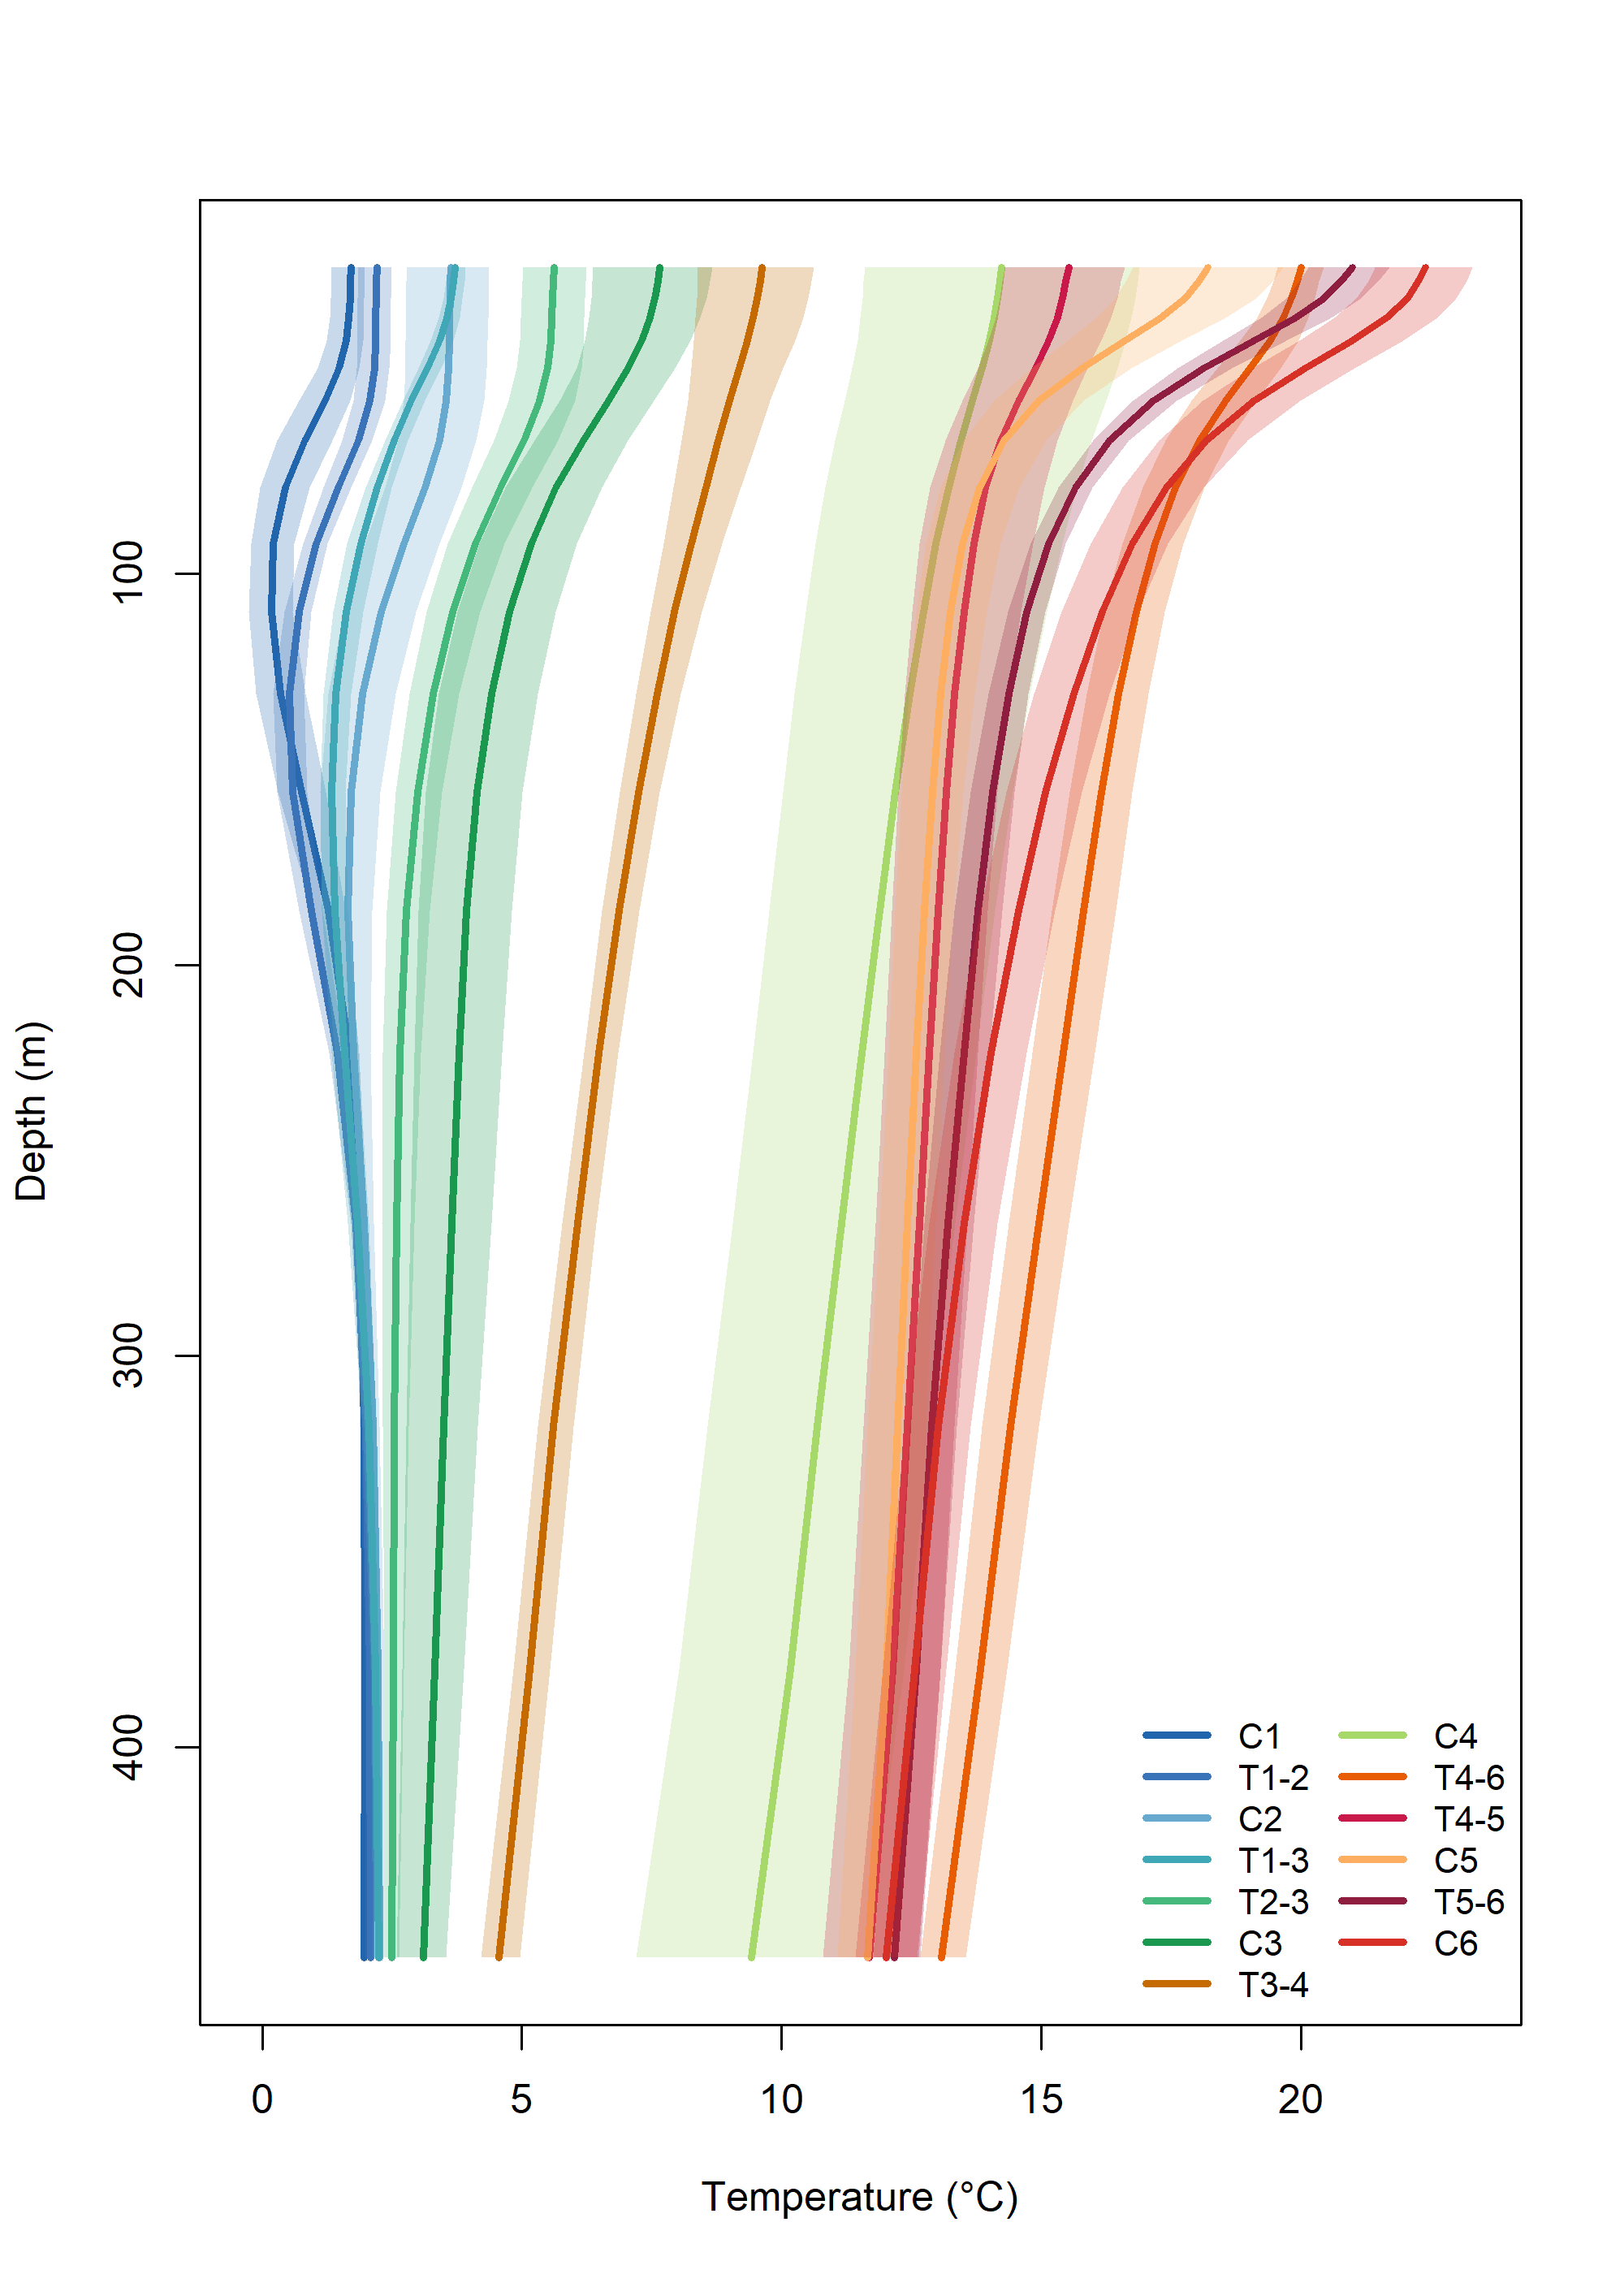
\includegraphics[width=\textwidth]{images/03_methodology/temperature_clusters_transitions}
			\caption{Profil de température (°C) moyen par cluster}
			\label{fig:temperatureclusterstransitions_a}
		\end{subfigure}
		\hfill
		\begin{subfigure}[b]{0.48\textwidth}
			\centering
			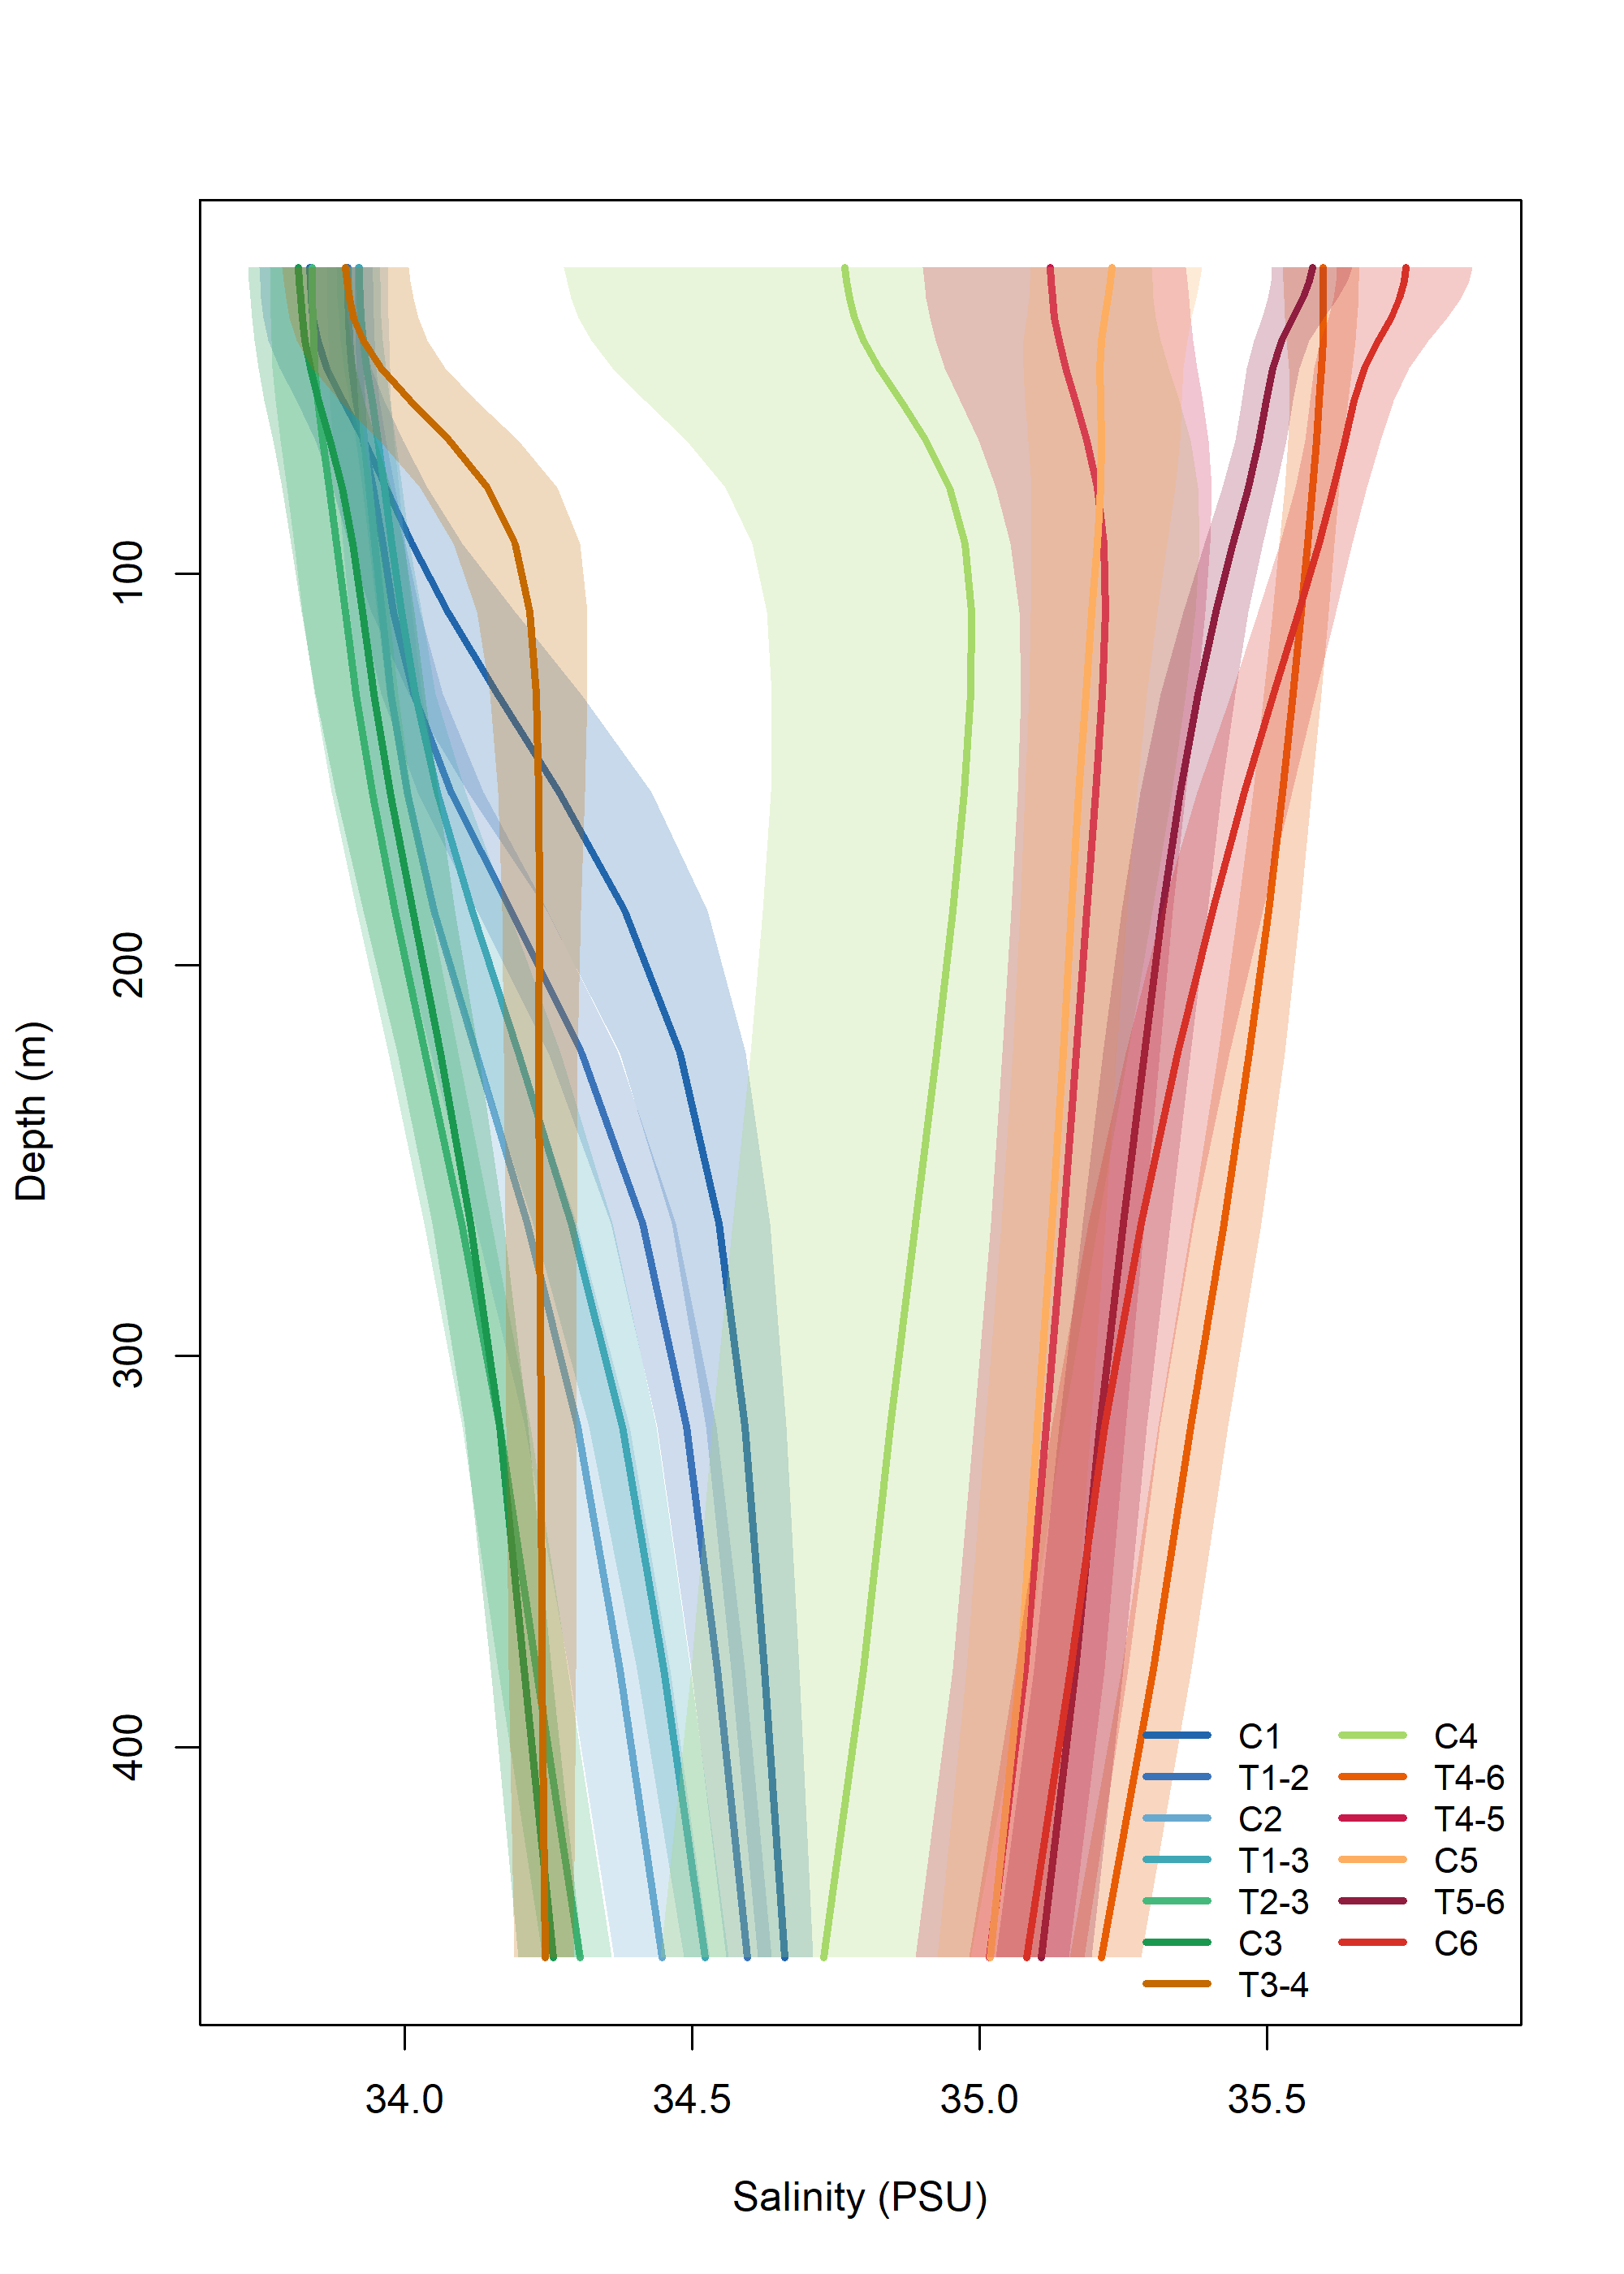
\includegraphics[width=\textwidth]{images/03_methodology/salinity_clusters_transitions}
			\caption{Profil de salinité (PSU) moyen par cluster}
			\label{fig:temperatureclusterstransitions_b}
		\end{subfigure}
		\caption{}
		\label{fig:temperatureclusterstransitions}
	\end{figure}
	
	Les FOD correspondent alors à des masses d'eau ayant des propriétés thermohalines similaires et permettent de visualiser l'hydrodynamisme de la région (tourbillons emprisonnant les masses d'eau en leurs coeur, filaments, fronts), voir figure \ref{fig:comparaisondofmap}. Historiquement, la zone d'étude était régionalisée selon l'apport d'eau de glace. On mentionne les Coastal and Continental Shelf Zone (CCSZ), Seasonal Ice Zone (SIZ), Permanently Open Ocean Zone (POOZ), Polar Frontal Zone (PFZ) ou Sub-Antarctic Zone (SAZ) \cite{treguer1992}. Plus récemment, les termes de WIZ (Winter Ice Zone) et MIEZ (Maximum Ice Extent Zone) ont également été introduits \cite{adroli2026}. En effet, ces zones présentent des régimes de productivité très différents. Travailler avec les FOD permet de retrouver cette régionalisation puisque chaque cluster encode les caractéristiques thermohaline de l'eau et donc encode l'adoucissement de l'eau due à la fonte des glaces. La seule exception concerne la SZ : cette zone est marquée par des apports minéraux et en fer d'origine continentale (mise en suspension de sédiments du plateau, fonte glaciaire). Ces processus, propres au domaine côtier, ne sont pas capturés par notre modèle de régionalisation, fondé uniquement sur les propriétés thermohalines des masses d'eau.
		
	\subsection{Colocalisation NASC/PIG/FTLE/FOD}
	Afin d'étudier la relation entre la distribution des organismes détectés acoustiquement (NASC), la dynamique de surface, les conditions hydrologiques et l'activité phytoplanctonique; les données de NASC ont été colocalisées avec lese \textit{Finite-Time Lyapunov Exponents} (FTLE), les \textit{concentration pigmentaire} (PIGMeANN) et les \textit{Domaine Océanographique Fonctionnel }(FOD).
	
	Le jeu de données d'acoustique active contient, pour chaque unité élémentaire d'échantillonnage (ESU), la date et l'heure d'acquisition, ses coordonnées géographiques (latitude et longitude) et la valeur de NASC associée (calculée à partir du volume de rétropropagation $S_v$).
	
	Les données environnementales sont fournies sous la forme de grilles spatiales, principalement organisées en fichiers NetCDF journaliers. Pour chaque fréquence acoustique considérée (38 et 120 kHz), les dates présentes dans le jeu de données acoustique sont identifiées. Pour chacune de ces dates, les données environnementales correspondantes sont recherchées et chargées afin d'être associées aux observations acoustiques.
	
	La colocalisation repose sur une correspondance temporelle à l'échelle journalière et sur une association spatiale par la méthode du plus proche voisin. Pour chaque ESU, ses coordonnées géographiques sont comparées aux coordonnées de la grille spatiale de chacune des variables environnementales. Le pixel dont les coordonnées sont les plus proches de celles de l'ESU est alors sélectionné. Cette recherche est effectuée indépendamment selon les dimensions de latitude et de longitude :

	\begin{equation}
		i_{\mathrm{lon}} =
		\underset{i}{\operatorname{argmin}}
		\left|
		\mathrm{lon}_{X,i} -
		\mathrm{lon}_{\mathrm{ESU}}
		\right|
	\end{equation}
	
	et
	
	\begin{equation}
		i_{\mathrm{lat}} =
		\underset{i}{\operatorname{argmin}}
		\left|
		\mathrm{lat}_{X,i} -
		\mathrm{lat}_{\mathrm{ESU}}
		\right|
	\end{equation}

	
	
	où $\mathrm{lon}_{X,i}$ et $\mathrm{lat}_{X,i}$ correspondent respectivement aux coordonnées de longitude et de latitude de la grille de la variable environnementale $X$ considérée.
	
	La valeur environnementale associée à chaque ESU est ensuite extraite au niveau du pixel correspondant aux indices sélectionnés :
	\begin{equation}
		X(i_{\mathrm{lon}},i_{\mathrm{lat}}),
	\end{equation}
	
	où $X$ représente l'une des variables environnementales considérées (FTLE, PIGMeANN ou FOD).
	
	Cette procédure est appliquée indépendamment à chaque variable environnementale. Les données finales permettent ainsi d'associer, à chaque ESU acoustique, sa position géographique, sa date d'acquisition, sa valeur de NASC ainsi que les valeurs des différentes variables environnementales correspondantes (FTLE, PIGMeANN et FOD). Ce jeu de données colocalisé constitue la base des analyses par machine learning visant à étudier les relations entre la distribution acoustique des organismes et les caractéristiques de leur environnement.
	
	\section{Décrire la structuration des communautés phytoplanctoniques de la région}
	\label{section:pigs}
	Cette section décris la méthode effectuée pour comprendre comment groupes d'rganismes photosynthétiques (PFD et PSC) sont structurés spatio-temporellement. 
	
	Dans un premier temps, les données pigmentaires (en ratio) de toute la région d'étude ([45, 90]°E de longitude, [-30, -60]°N de latitude) ont été extraits. On obtient une matrice $pigs = \mathbb{R}^{dates \times npigments \times lon \times lat}$ (npigments = 9, voir \ref{tab:pigments}) sur laquelle on effetcue une Analyse pas Composante Principale. On regroupe ensuite les données similaires avec un clustering de type k-means (nclust = 6, choix par méthode du coude, voir Annexe \ref{annexe : cluster_pig}, figure \ref{fig:elbowmethodkmeans}) sur les 7 premières composantes principales (>=97.7\% expl. var., voir Annexe \ref{annexe : cluster_pig}, figure \ref{fig:explainedvarpig})). Des analyses de distributions des ratios de concentration de pigments sont ensuite réalisées afin d'étudier la composition pigmentaire de chaque communauté. Finalement, afin de comprendre la structure spatiale et temporelle des communautés, les clusters sont projetés sur des cartes journalières et totales (avec un indice de pureté associé). 
	
	
	\section{Prédire le NASC en fonction de variables environnementals : arbres de régression}
	Cette section décrit comment nous avons cherché à (1) identifier la structure prédictive du NASC à partir des variables environnementales (FOD, FTLE) et phytoplanctoniques, et (2) étudier les relations structurelles entre le NASC et ces variables prédictives (FOD, ratios de pigments, FTLE). Pour cela, nous avons utilisé trois modèles d'arbres de régression : CART, Random Forest et XGBoost. Ces modèles ont été choisis pour leurs propriétés complémentaires et leur gestion différente du compromis biais-variance, inhérent à tout problème d'apprentissage automatique.
	
	%"Depending on the problem, the basic purpose of a classification/regression study can be either to produce an accurate classifier or to uncover the predictive structure of the problem." (classif. and regression trees p.6)
	%Notre objectif ici est chercher à connaître la prédictibilié du NASC en fonction de la structure des communautés phytoplanctoniques, en lien avec l'activité de mésoéchelle. The goal is to understand the structural relationship between  the response and the measured variables. (p.221)


	\subsection{Description des modèles}
	\subsubsection{Classification and Regression Trees (CART)}
	Le modèle CART \cite{breiman1984classification} construit un arbre de décision par partitionnement binaire récursif de l'espace des variables explicatives. À chaque nœud, l'algorithme sélectionne la variable et le seuil de coupure qui minimisent le plus la variance intra-groupe des sous-ensembles résultants (critère d'impureté : réduction de la somme des carrés des résidus). Ce processus est répété récursivement jusqu'à ce qu'un critère d'arrêt soit atteint : profondeur maximale de l'arbre (\texttt{maxdepth}), nombre minimal d'observations requis pour tenter un nouveau split (\texttt{minsplit}), ou gain d'impureté insuffisant pour justifier une division supplémentaire (\texttt{cp}, paramètre de complexité). La prédiction d'une nouvelle observation correspond à la moyenne des valeurs observées dans la feuille terminale où elle est routée.
	
	Un arbre unique est un modèle à faible biais mais à forte variance : sans contrainte de régularisation, il peut s'ajuster jusqu'à isoler chaque observation d'entraînement dans sa propre feuille (biais faible, mais surapprentissage possible et forte sensibilité à toute perturbation du jeu de données d'entraînement). Les hyperparamètres \texttt{cp}, \texttt{minsplit} et \texttt{maxdepth} contrôlent directement ce compromis en limitant la profondeur/complexité de l'arbre. CART est se démarque des autres méthodes par sa forte interprétabilité : la structure de l'arbre est directement lisible comme une succession de règles de décision.
	
	\subsubsection{Random Forest (RF)}
	Le Random Forest \cite{breiman2001random} est un ensemble de $B$ arbres CART entraînés indépendamment et dont les prédictions sont moyennées. Deux sources de randomisation permettent de décorréler les arbres entre eux :
	\begin{itemize}
		\item \textbf{Bagging} (bootstrap aggregating) : chaque arbre est entraîné sur un échantillon bootstrap (tirage aléatoire avec remise) du jeu d'entraînement, de même taille que celui-ci.
		\item \textbf{Sous-échantillonnage des variables} : à chaque split, seul un sous-ensemble de \texttt{mtry} variables (tirées aléatoirement parmi l'ensemble des covariables) est considéré comme candidat à la division, plutôt que la totalité des variables disponibles.
	\end{itemize}
	
	Cette double randomisation maximise la diversité entre arbres et empêche l'obtention d'une forêt d'arbres quasi identiques et fortement corrélés, ce qui serait le cas si chaque arbre avait accès à l'intégralité des données et des variables à chaque split. Or, la réduction de variance obtenue en moyennant $B$ estimateurs n'a lieu que si ces estimateurs sont peu corrélés entre eux : moyenner des arbres corrélés apporte un gain de variance bien plus limité que moyenner des arbres indépendants. Random Forest permet ainsi de conserver le faible biais propre aux arbres de décision profonds tout en réduisant fortement leur variance individuelle, sans nécessiter la même régularisation stricte qu'un CART isolé. Les hyperparamètres \texttt{mtry} (nombre de variables candidates par split) et \texttt{min.node.size} (taille minimale des feuilles) contrôlent la profondeur/complexité de chaque arbre individuel, tandis que \texttt{num.trees} fixe la taille de l'ensemble. Un nombre d'arbres insuffisant ne permet pas à la réduction de variance par moyennage de converger, tandis qu'au-delà d'un certain seuil, l'ajout d'arbres supplémentaires n'apporte plus de gain significatif.
	
	\subsubsection{XGBoost}
	XGBoost (Extreme Gradient Boosting) \cite{chen2016xgboost} est une méthode d'ensemble séquentielle, par opposition au moyennage parallèle du Random Forest (bagging). Les arbres sont construits un à un, chaque nouvel arbre étant entraîné pour corriger les erreurs résiduelles de l'ensemble des arbres précédents. La prédiction finale correspond à la somme pondérée des contributions de tous les arbres de la séquence.
	
	Contrairement au bagging, où chaque estimateur est indépendant et où l'objectif est de réduire la variance sans biaiser l'estimateur moyen, le boosting réduit progressivement le biais de l'ensemble à chaque itération, celà au prix d'un risque de surapprentissage croissant avec le nombre d'itérations. XGBoost intègre plusieurs mécanismes de régularisation pour limiter ce risque : un taux d'apprentissage (\texttt{eta}) qui pondère la contribution de chaque nouvel arbre (un taux faible ralentit la convergence mais limite le surapprentissage), une profondeur maximale par arbre (\texttt{max\_depth}), un poids minimal d'observations requis par feuille (\texttt{min\_child\_weight}), ainsi qu'un sous-échantillonnage des observations et des variables à chaque itération (\texttt{subsample}, \texttt{colsample\_bytree}). Le nombre d'itérations de boosting (\texttt{nrounds}) est un hyperparamètre particulièrement sensible : trop faible, l'ensemble sous-ajuste (biais élevé) ; trop élevé, il surapprend le jeu d'entraînement (variance élevée).
	
	\subsection{Calcul de l'importance des variables}
	L'importance d'une variable explicative quantifie sa contribution à la qualité des prédictions du modèle. LesCART, Random Forest et XGBoost ne calculent pas cette quantité de la même manière et les valeurs obtenues ne sont donc pas directement comparables entre modèles (ni en échelle, ni en unité), même si elles peuvent l'être entre schémas de validation croisée ou fréquences pour un même modèle.
	
	\subsubsection{CART}
	Pour un arbre de décision unique, l'importance d'une variable est calculée comme la somme, sur l'ensemble des nœuds où cette variable est utilisée comme critère de split, de la réduction d'impureté qu'elle apporte (la RSS dans notre cas) \cite{breiman1984classification}. Une variable qui n'intervient dans aucun split de l'arbre final a une importance nulle. Cette mesure est directement issue de la structure de l'arbre entraîné (fonction \texttt{variable.importance} du package \texttt{rpart}) et ne nécessite aucun calcul supplémentaire après l'entraînement.
	
	\subsubsection{Random Forest}
	Random Forest utilise l'\textbf{importance par permutation} \cite{breiman2001random}, calculée pour chaque arbre de la forêt sur ses observations out-of-bag (OOB, celles non tirées dans l'échantillon bootstrap de cet arbre) : on calcule l'erreur de prédiction OOB du modèle, puis on permute aléatoirement les valeurs d'une variable donnée entre les observations OOB et on recalcule l'erreur. L'importance de cette variable correspond à l'augmentation moyenne de l'erreur (ici, l'augmentation du MSE) causée par cette permutation, moyennée sur l'ensemble des arbres de la forêt \cite{wright2017ranger}. Une variable dont la permutation n'affecte pas (ou peu) la performance du modèle a une importance faible ou nulle (contrairement à une variable dont le modèle dépend fortement). Cette méthode a été préférée à l'importance par impureté (\textit{Gini/RSS importance}, analogue à celle de CART mais moyennée sur tous les arbres), car elle est moins sensible aux biais liés à l'échelle ou à la cardinalité des variables \cite{strobl2007bias}.
	
	\subsubsection{XGBoost}
	L'importance des variables dans XGBoost est calculée à partir du Gain : pour chaque split de chaque arbre de la séquence de boosting, on calcule la réduction de la fonction de perte qu'il apporte. Le Gain d'une variable est la somme de ces réductions sur tous les splits où elle est utilisée, sur l'ensemble des arbres \cite{chen2016xgboost}. Cette mesure est directement disponible en sortie du modèle entraîné (fonction \texttt{xgb.importance}) sans calcul supplémentaire.
	
	Le Gain présente cependant deux limites : il ne renseigne pas sur le sens de l'effet d'une variable (contribution positive ou négative à la prédiction), et il répartit arbitrairement le crédit entre variables fortement corrélées. 
	
	\subsection{Schéma de validation, Tuning, entraînement et prédiction}
	
	\subsubsection{Proximité spatio-temporelle et dépendance spatiale des données}
	Les données environnementales et biologiques présentent une structuration dépendante de la latitude. Les hypothèses de stationnarité d'ordre 1 et 2 ne sont donc pas respectées. 
	De plus, lors des campagnes océanographiques, une onde acoustique est émise toutes les 3 à 4 secondes. La conséquence de cette proximité spatio-temporelle est la présence de pseudo-duplicatas dans le jeu de données. Cet élément est à prendre en considération lors de la construction du schéma de validation croisé afin d'obtenir un jeu de données de validation sans fuite du jeu de données d'entraînement (data leakage). 
	
	\subsubsection{Schémas de validation croisée}
	La validation croisée consiste à diviser l'ensemble des données en $K$ sous-ensemble de taille à peu près identiques, appelés \textit{folds}. 1 fold sert d'ensemble de validation/test et les $K-1$ folds restants servent d'ensemble d'entraînement. On obtient donc $K$ prédictions pour un même modèle. 
	
	Il existe différentes manières de sous-échantillonner les données pour construire les folds. Dans notre étude, nous avons testés différentes méthodes : Monte-Carlo CV et la validation croisée par blocking spatio-temporel.
	
	La \textbf{Monte Carlo Cross Validation} \cite{xu2004monte} (appelée aussi Repeated Random Sub-sampling Validation) consiste à effectuer K tirages aléatoires indépendants sur une certaine proportion $P$ des données pour sélectionner l'ensemble d'entraînement, la proportion de données restante sert d'ensemble de test \footnote{A noter que dans cette méthode, les tirages se chevauchent, ce n'est pas une partition exhaustive comme le K-fold CV}. Dans notre cas, la proportion de donnée d'entraînement choisie est $P=80$ \% et 20\% de test. Le nombre de fold a été fixé arbitrairement à $K =  10$.
	
	La \textbf{validation croisée par blocking spatio-temporel} \cite{roberts2017crossvalidation} consiste à partitionner l'espace (ou le temps) selon une grille de résolution choisie. Elle permet de limiter la fuite de données (dataleakage) et les effets de la dépendance spatio-temporelle. Le sous-échantillonage est choisi en isolant un block de cette grille (le bloc test), les blocs situés dans un rayon tampon (buffer) autour de ce bloc sont exclus de l'entraînement et les blocs restants (hors buffer) servent d'ensemble d'entraînement. Dans notre cas, plusieurs résolution ont été retenues : 1500km de longitude x 1000km de latitude, 200 km x 200 km, 20 km x 20 km et 1 journée (selon les tests effectués, voir annexe \ref{annexe:choix_valid_croisee_autocorr}). Dans ce schéma de validation croisée, le nombre de fold dépend de la résolution de la grille spatio-temporelle choisie. Ici nous avons déterminé le nombre de folds en procédant comme suis : après avoir découpé l'espace (ou le temps) en une grille (de résolution choisie), on regarde le nombre de points que contiennent chaque cellule et on garde les cellules (nombre de blocks éligibles) avec un nombre de point supérieur à $n=50$ points. Le nombre de folds correspond alors à 30 \% du nombre de blocs éligibles, plafonnée à un maximum de 30 folds et à un minimum de 5 folds, sans jamais dépasser le nombre de blocs réellement éligibles disponibles. Le nombre de fold pour XGB diffère à cause du nombre de données supérieures utilisé dans cette méthode qui tolère les valeurs manquantes. Le choix des folds a également été contraint par la latitude pour forcer une représentation homogène des données selon cet axe.
	
	\begin{table}[htbp]
		\centering
		\caption{Schémas de validation croisée et nombre de folds retenus (38 kHz)}
		\label{tab:cv_schemes}
		\small
		\begin{tabularx}{\textwidth}{@{} l l r r r X @{}}
			\toprule
			Schéma & Sous-ensemble & Buffer & Blocs disp. & Folds retenus \\
			\midrule
			Naive RS 80/20 (Monte Carlo) & CART/RF/XGB & -- & -- & 10 \\
			\midrule
			Bloc spatial 1500$\times$1000\,km & CART/RF & 100\,km & 6   & 5 \\
			Bloc spatial 1500$\times$1000\,km & XGB     & 100\,km & 9   & 5 \\
			\midrule
			Bloc spatial 200$\times$200\,km & CART/RF & 20\,km & 24  & 7 \\
			Bloc spatial 200$\times$200\,km & XGB     & 20\,km & 76  & 23 \\
			\midrule
			Bloc spatial 20$\times$20\,km & CART/RF & 5\,km & 106 & 30 \\
			Bloc spatial 20$\times$20\,km & XGB     & 5\,km & 663 & 30 \\
			\midrule
			Bloc temporel 1 jour & CART/RF & 1 jour & 19  & 6   \\
			Bloc temporel 1 jour & XGB     & 1 jour & 81  & 24  \\
			\bottomrule
		\end{tabularx}
	\end{table}
	
	\subsubsection{Tuning}
	Etant donné le nombre important de modèles ($3 \text{ modèles } \times 5 \text{ schémas de validation croisée } \times \text{ K folds } \times 2 \text{ fréquences}$), seule une petite grille de tuning des hyperparamètres a été utilisée (voir tableau \ref{tab:tuning_grids}). On retient les hyperparamètres qui minimisent la RMSE test moyenne inter-fold. Une exception est faite pour le tuning du modèle XGBoost, le paramètre \texttt{nrounds} est optimisé ici par early stopping plutôt que par recherche sur grille : l'entraînement est interrompu dès que le RMSE de validation cesse de s'améliorer pendant un nombre d'itérations consécutives fixé (patience).
	
		\begin{table}[htbp]
			\centering
			\caption{Grilles d'hyperparamètres testées lors du tuning}
			\label{tab:tuning_grids}
			\begin{tabularx}{\textwidth}{l l X r}
				\toprule
				Modèle & Hyperparamètre & Valeurs testées & Comb. \\
				\midrule
				\multirow{3}{*}{CART}
				& \texttt{cp}        & 0.0005 ; 0.001 ; 0.005 ; 0.01 & \multirow{3}{*}{36} \\
				& \texttt{minsplit}  & 10 ; 20 ; 40                  & \\
				& \texttt{maxdepth}  & 5 ; 10 ; 15                   & \\
				\midrule
				\multirow{3}{*}{RF (ranger)}
				& \texttt{mtry}           & 2 ; 3 ; 4      & \multirow{3}{*}{18} \\
				& \texttt{min.node.size}  & 5 ; 10 ; 20    & \\
				& \texttt{num.trees}      & 300 ; 500      & \\
				\midrule
				\multirow{4}{*}{XGBoost}
				& \texttt{max\_depth}         & 3 ; 4 ; 6          & \multirow{4}{*}{27} \\
				& \texttt{eta}                & 0.01 ; 0.05 ; 0.1  & \\
				& \texttt{min\_child\_weight} & 1 ; 3 ; 5           & \\
				& \texttt{nrounds}            & optimisé par \emph{early stopping} (max. 1000, patience 20) & \\
				\bottomrule
			\end{tabularx}
		\end{table}
		
		\subsubsection{Entraînement et prédiction}
		Chaque fold de chaque modèle est entraîné indépendamment avec les meilleurs paramètres obtenus par le tuning (voir annexe \ref{annexe:tuning_res}) et les métriques associées (R², RMSE, résidus) sont calculées. La prédiction finale d'un modèle correspond à la moyenne des prédictions des $K$ folds de ce modèle.
		
		Une carte de prédiction est ensuite générée à partir des données de variables environnementales de toute la ROI (FOD, concentrations de pigments)\footnote{Cet ensemble de donnée diffère de l'ensemble d'entraînement qui contient uniquement les valeurs des variables environnementales associées aux points de coordonnée longitude/latitude du transect de la campagne océanographique collectant les données d'acoustiques qu'on prédit}. 
		
		
	
	
	
	\clearpage
	\chapter{Résultats}
	\section{Distributions des variables étudiées}
	\subsection{Concentrations de pigments photosynthétiques}
	\label{res:distribs_pigs}
	On s'intéresse ici aux distributions inter-annuelles des contributions de chaque pigment (et donc chaque PFD) sur la production primaire totale.
	La Fucoxantine, pigment associé aux diatomée, diminue progressivement entre 2018 et 2022 de manière significative puis retrouve une contribution identique à celle de 2018 (voir figure \ref{fig:violininterannualratiospigmenttotpig}). La contribution du 19'-hexanoyloxyfucoxantine, associée aux haptophytes, est stable entre 2018 et 2022 et augmente légèrement, mais significativement en 2023. Le 19'butanoyloxyfucoxantine diminue faiblement entre 2018 et 2023. On n'observe pas de tendance claire et significative pour les autres pigments.
	Concernant la Chlorophylle-a, sa concentration diminue significativement entre 2018 et 2021 puis se stabilise \ref{fig:violininterannualchlaa}.
	
		\begin{figure}[H]
			\centering
			
\includegraphics[width=\textwidth]{images/04_resultats/01_distrib_ftle_nasc_ratio_chla/distrib_ftle_nasc_pig_interannual/violin_interannual_ratios_pigment_totpig}
			\caption{Distributions interanuelles (2018, 2021, 2022, 2023) estivales (janvier-mars) des contributions des pigments photosynthétiques dans la concentration de pigments photosynthétique totale, estimés à partir de l'algorithme PIGMeANN}
			\label{fig:violininterannualratiospigmenttotpig}
		\end{figure}
		
		\begin{figure}[H]
			\centering
			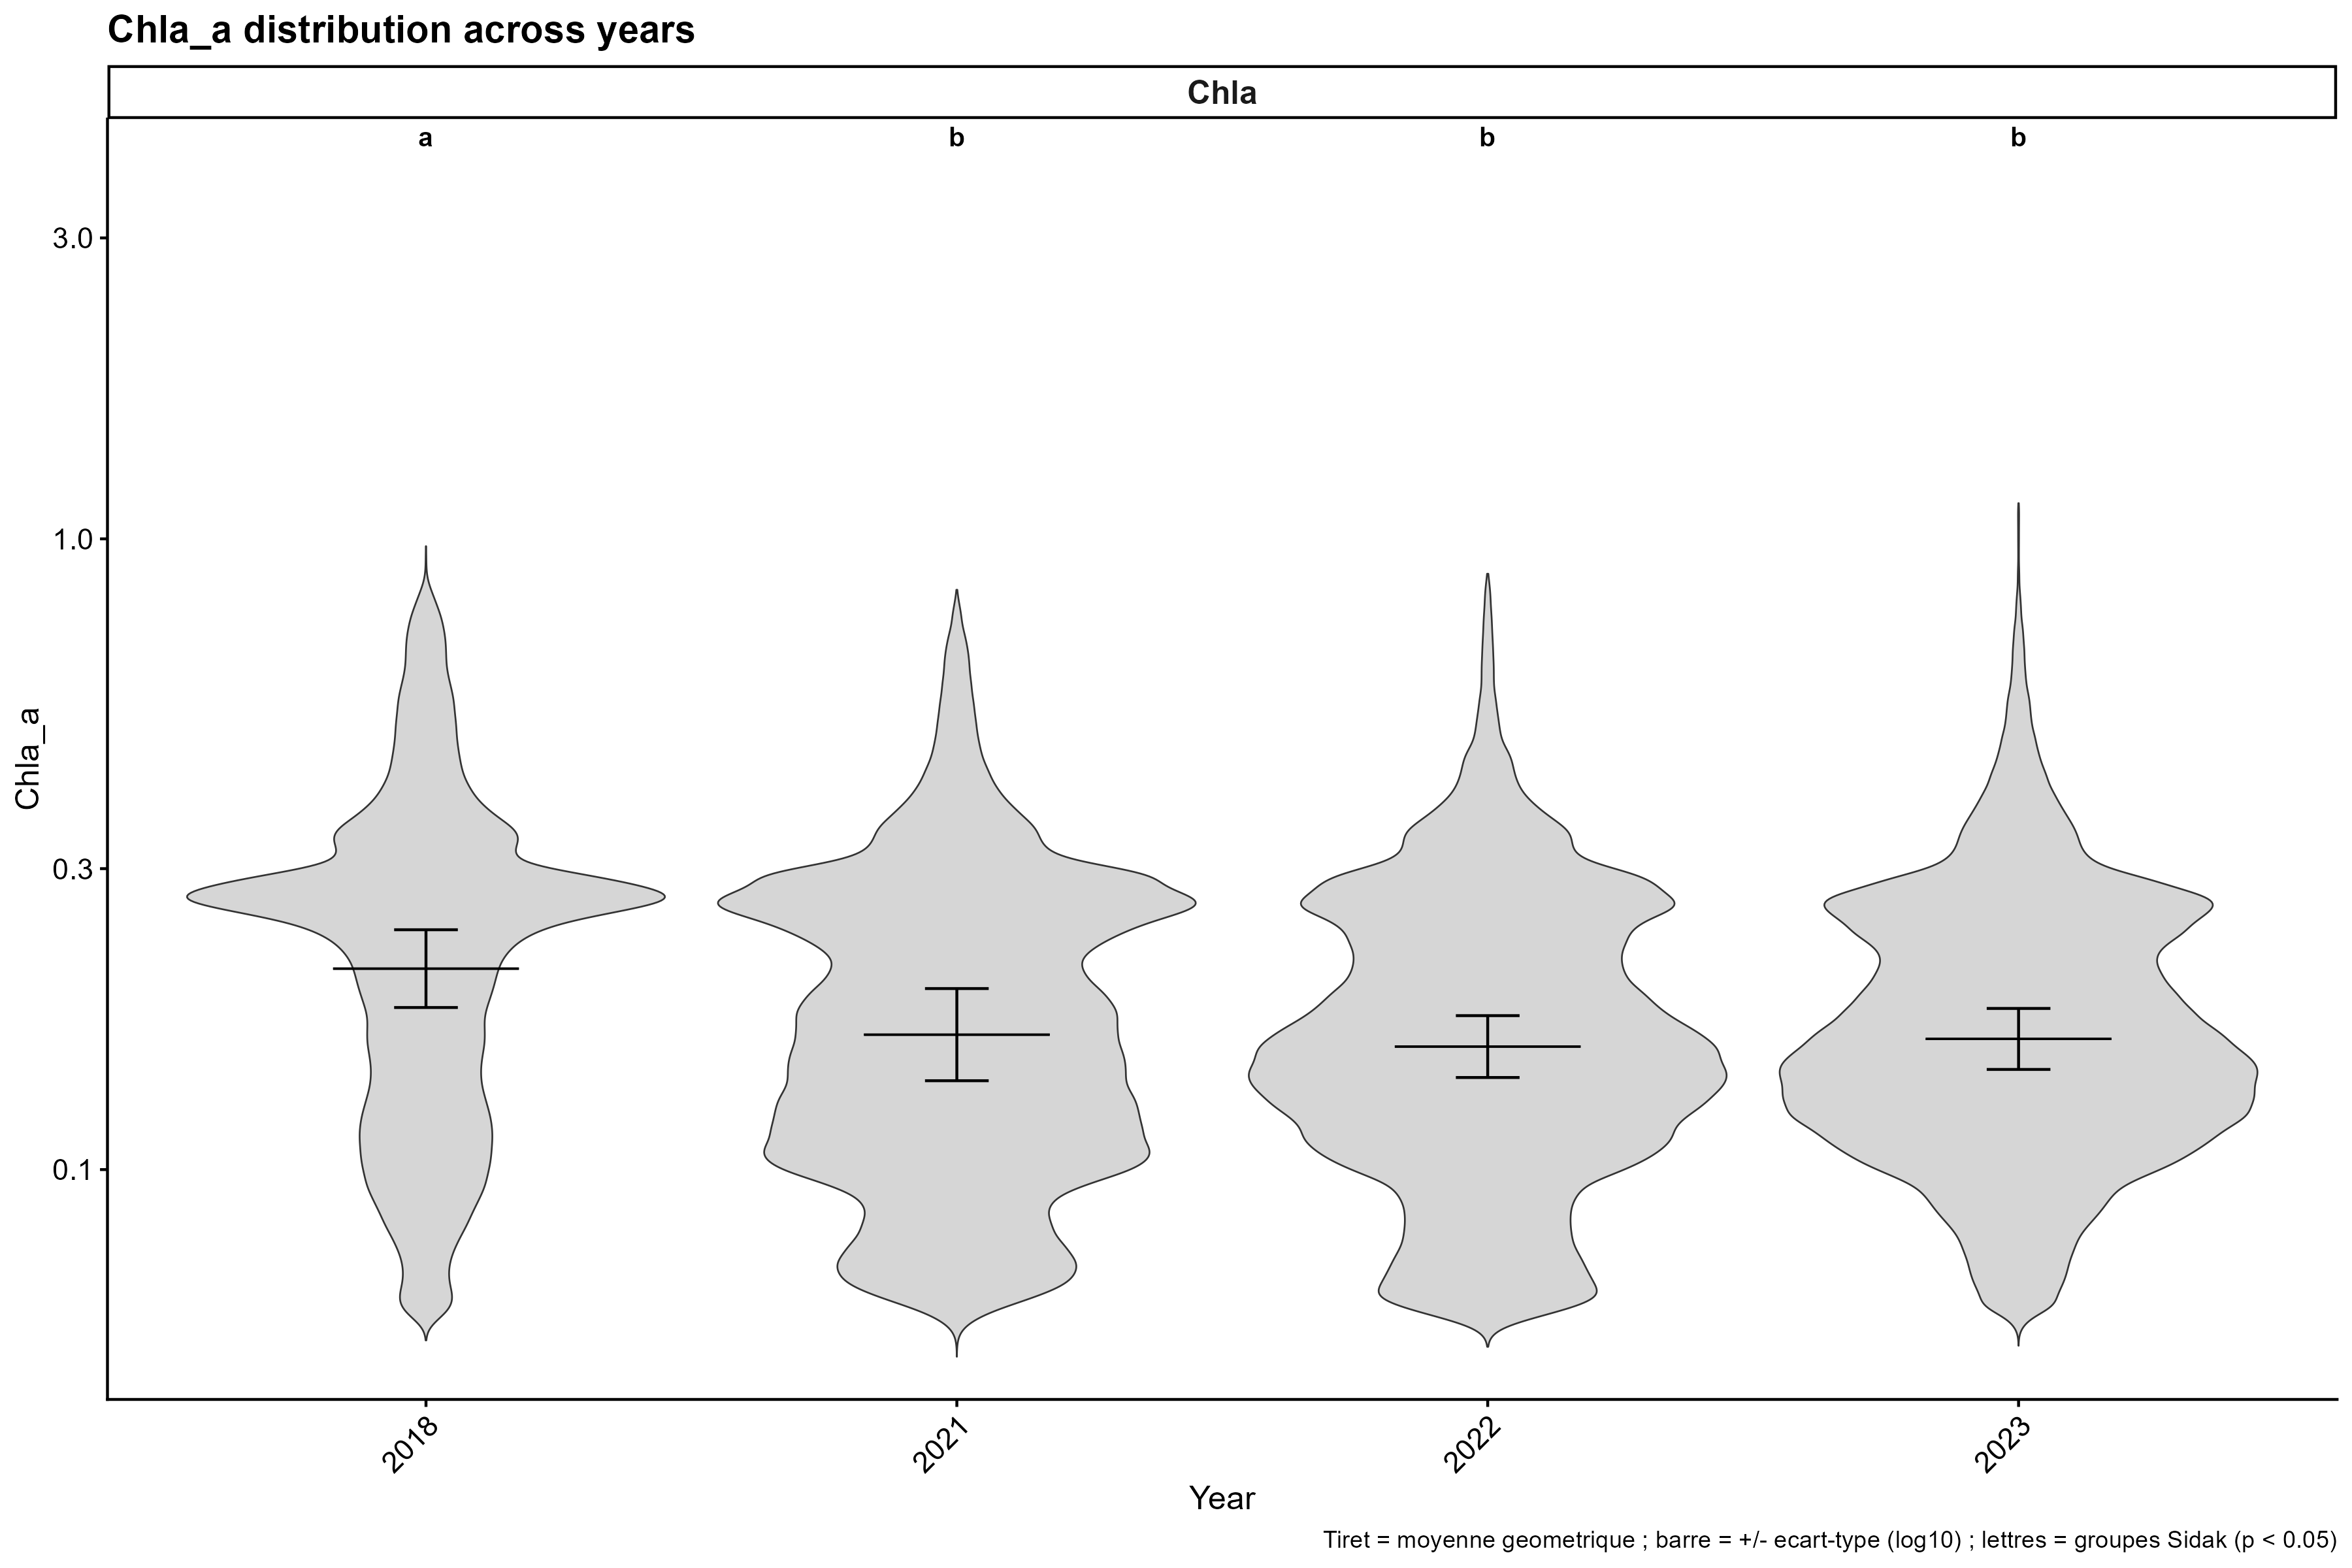
\includegraphics[width=0.8\textwidth]{images/04_resultats/01_distrib_ftle_nasc_ratio_chla/distrib_ftle_nasc_pig_interannual/violin_interannual_Chla_a}
			\caption{Distributions interanuelles (2018, 2021, 2022, 2023) estivales (janvier-mars) de la concentration en Chlorophylle-a, estimée par l'algorithme PIGMeANN}
			\label{fig:violininterannualchlaa}
		\end{figure}
		
	\subsection{Finite-Time Lyapunov Exponant}
		L'hydrodynamisme de la région, plus particulièrement la convergence/divergence des trajectoires de particules d'eau caractérisée par les FTLE diminue légèrement et de manière continue entre 2018 et 2023.
		
		\begin{figure}[H]
			\centering
			
\includegraphics[width=0.7\textwidth]{images/04_resultats/01_distrib_ftle_nasc_ratio_chla/distrib_ftle_nasc_pig_interannual/violin_interannual_FTLE}
			\caption{Distributions interanuelles (2018, 2021, 2022, 2023) estivales (janvier-mars) des Finite-Tile Lyapunov Exponent (FTLE) calculés à partir des données de courant CMEMS}
			\label{fig:violininterannualftle}
		\end{figure}
	
	
	\subsection{NASC}
	\label{res : distrib_nasc}
	Les biomasses de poissons pélagiques et d'euphausiacés sont caractérisées par acoutique active respectivement à 38 et 120 kHz. La biomasse de poissons pélagiques, sur les transects étudiés, augmente significativement entre 2018 et 2021 puis se stabilise  (figure \ref{fig:violininterannualnasc38khz}). La biomasse d'Euphausiacés est stable sur toute la période étudiée (figure \ref{fig:violininterannualnasc120khz})
	
	\begin{figure}[H]
		\centering
		
\includegraphics[width=0.7\textwidth]{images/04_resultats/01_distrib_ftle_nasc_ratio_chla/distrib_ftle_nasc_pig_interannual/violin_interannual_NASC__38_kHz_}
		\caption[Distribution du NASC (38 kHz) inter-annuelle (2018, 2021, 2022, 2023) estivale (janvier-mars) obtenus lors des campagnes océanographiques OBSAUSTRAL/THEMISTO]{Distribution du NASC inter-annuelle (2018, 2021, 2022, 2023) estivale (janvier-mars) obtenus lors des campagnes océanographiques OBSAUSTRAL/THEMISTO.}
		\label{fig:violininterannualnasc38khz}
	\end{figure}
	
	\begin{figure}[H]
		\centering
		
\includegraphics[width=0.7\textwidth]{images/04_resultats/01_distrib_ftle_nasc_ratio_chla/distrib_ftle_nasc_pig_interannual/violin_interannual_NASC__120_kHz_}
		\caption[Distribution du NASC (120 kHz) inter-annuelle (2018, 2021, 2022, 2023) estivale (janvier-mars) obtenus lors des campagnes océanographiques OBSAUSTRAL/THEMISTO]{Distribution du NASC inter-annuelle (2018, 2021, 2022, 2023) estivale (janvier-mars) obtenus lors des campagnes océanographiques OBSAUSTRAL/THEMISTO.}
		\label{fig:violininterannualnasc120khz}
	\end{figure}
	
	
	\section{Communautés phytoplanctoniques de la région d'étude}
	A partir de la méthode décrite \label{section:pig}, 6 communautés phytoplanctoniques ont été mises en évidence (figure \ref{fig:distributionpigmentscommunauteskmeansk6pftstats}). La communauté 4 est dominée par la contribution de la Zéaxanthine et de la Divinyl Chlorophylle-a, caractéristique des procaryotes picoplanctoniques et des cyanobactéries (voir tableau \ref{tab:pigments}). Les communautés 1, 3, 5 et 6 sont dominées par la contribution de la 19' hexanoyloxyfucoxantine et de la fucoxantine, typiquement associées à des diatomées et des haptophytes, organismes connus pour être en compétition dans cette région \cite{sari2025influence}.
	Elles diffèrent cependant entre elles (voir figure \ref{fig:distribpigmentsincommunauteskmeansk6pftstats}, Annexe \ref{annexe:distrib_commu_phyto}) par (1) leur intensité de biomasse totale (concentration de chlorophylle-a totale (chla\_total)), les communautés 1, 3, 6 sont associées a de fortes biomasses; (2) leur concentratione en 19' butanoyloxyfucoxantine, élevée dans la communauté 1 et 3; (3) La concentration en Alloxanthine, supérieure dans la communauté 6.
	\begin{figure}[H]
		\centering
		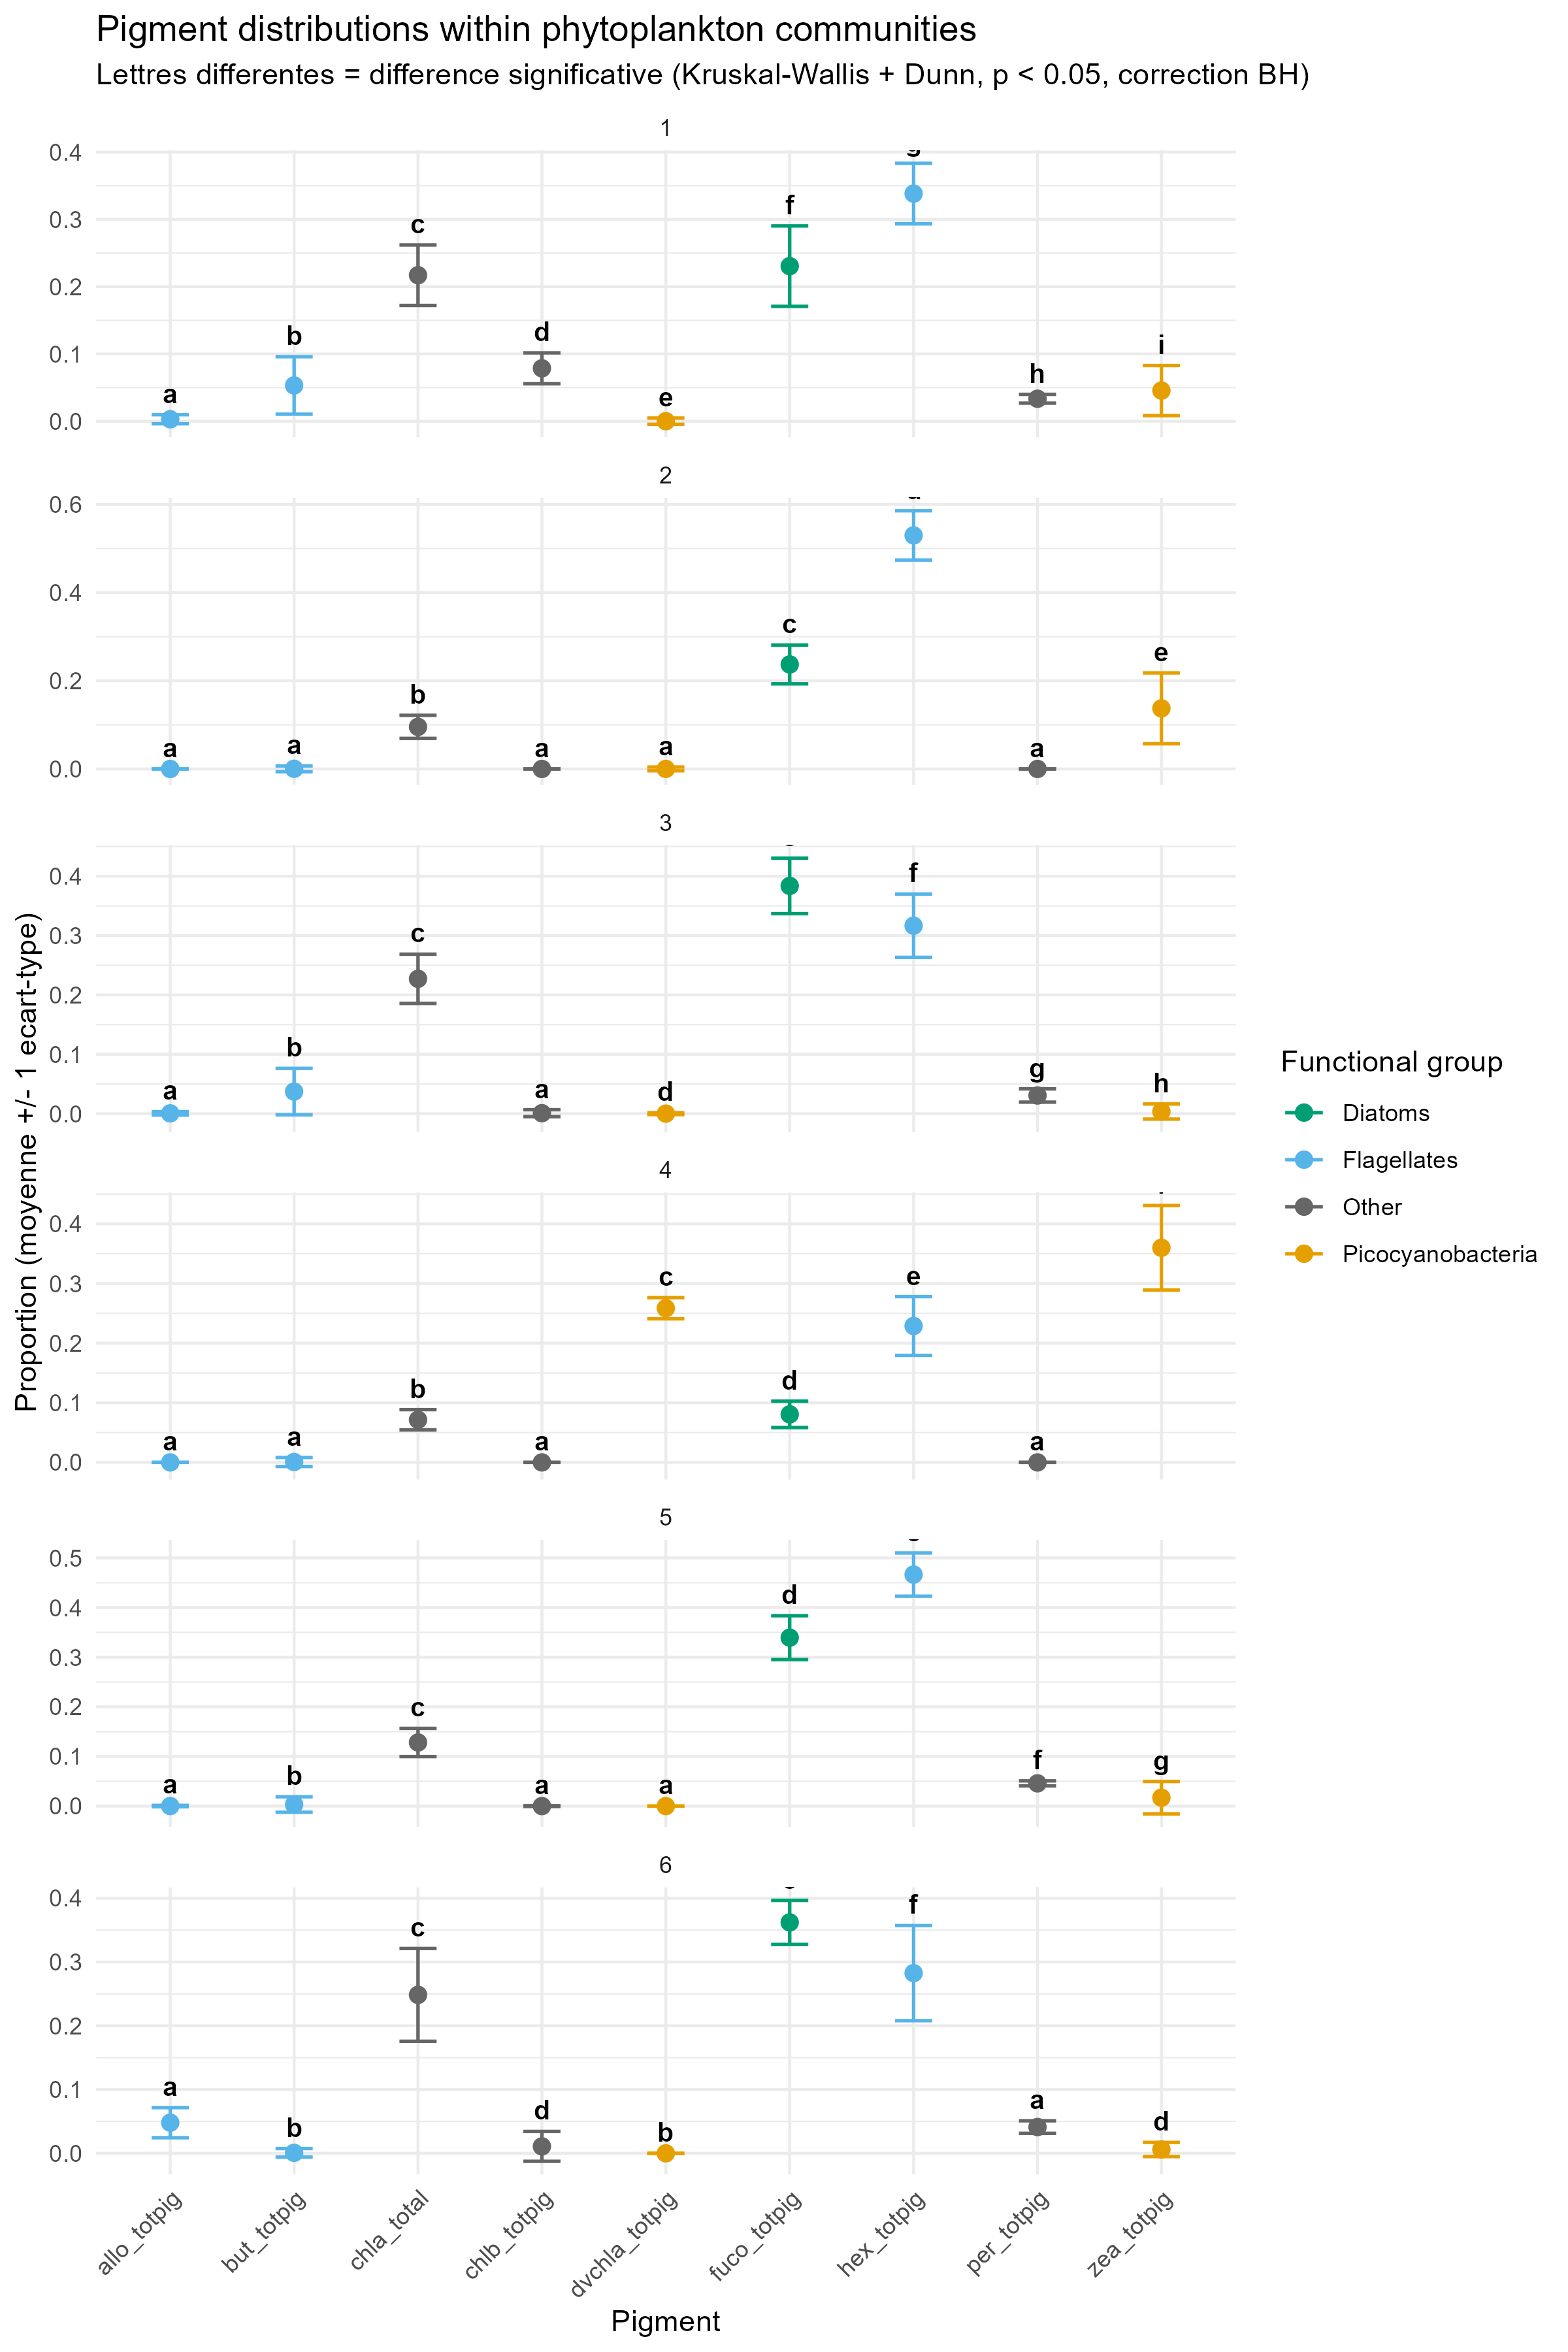
\includegraphics[width=\textwidth]{images/04_resultats/03_commu_phyto_cluster_pigs/distribution_pigments_communautes_kmeans_k6_PFT_stats}
		\caption{Distributions de la contribution des pigments (ratios) par cluster (communauté phytoplanctonique).}
		\label{fig:distributionpigmentscommunauteskmeansk6pftstats}
	\end{figure}
	
	\begin{figure}[H]
		\centering
		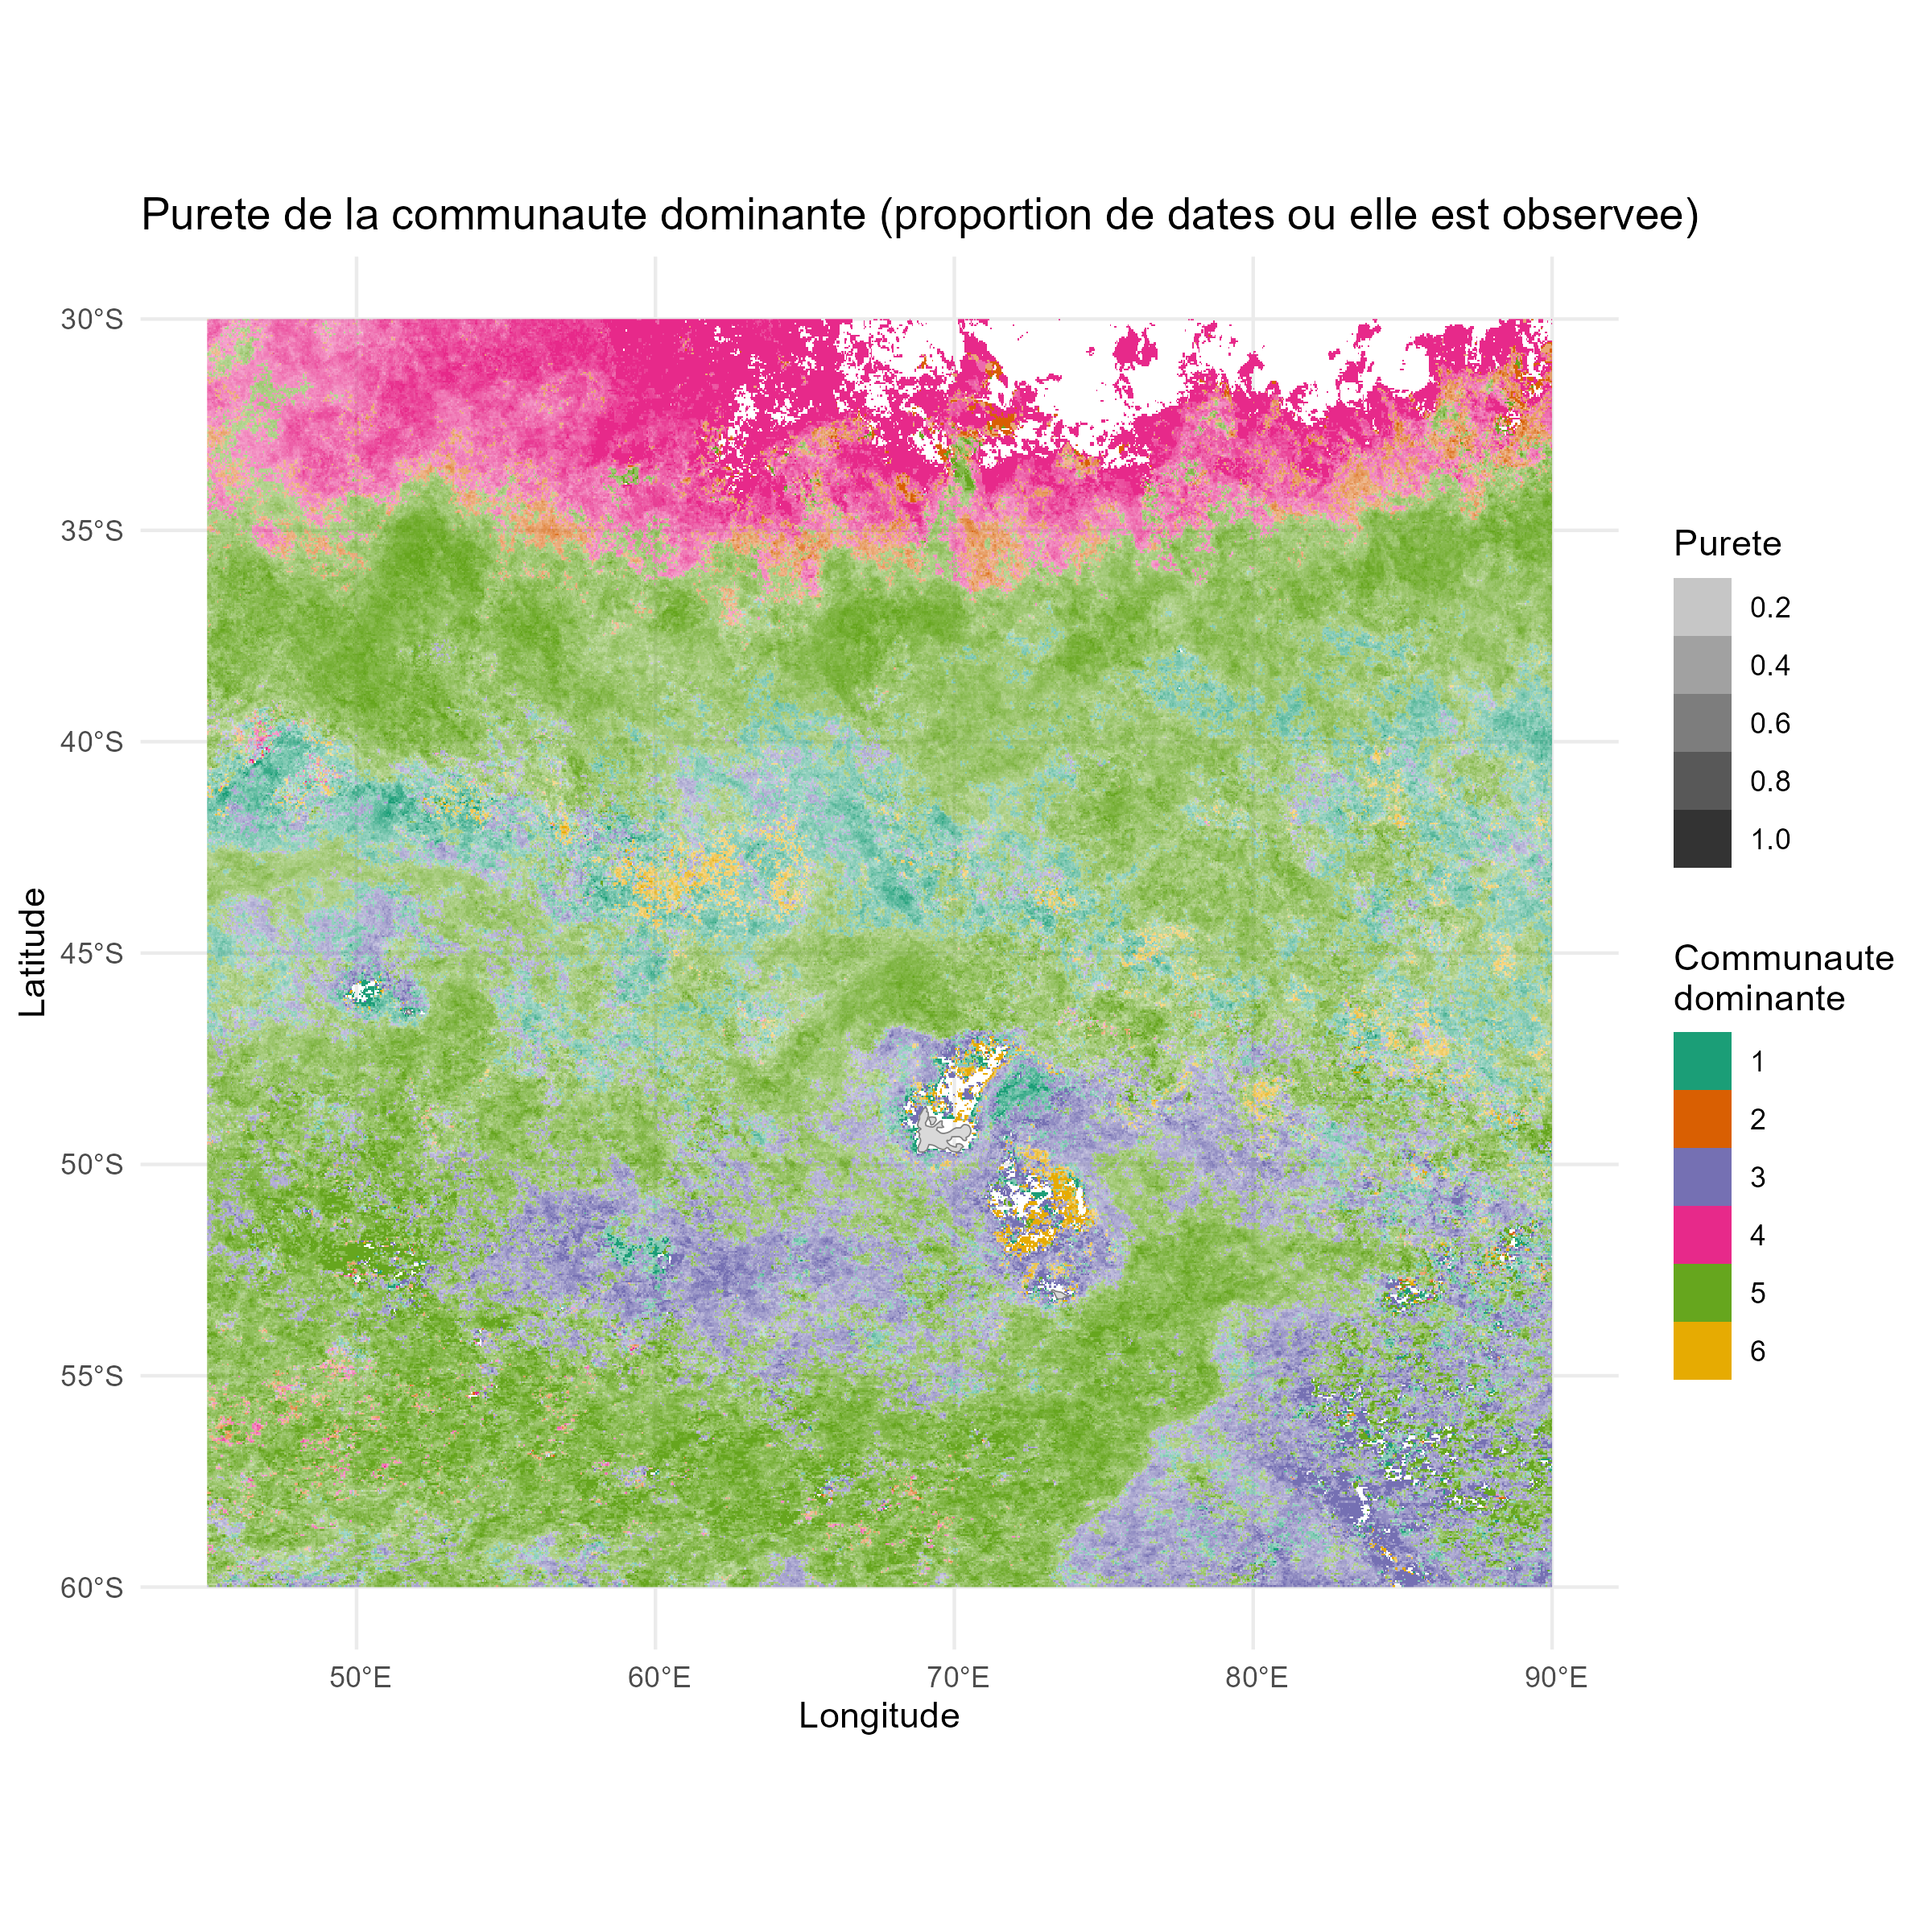
\includegraphics[width=\textwidth]{images/04_resultats/03_commu_phyto_cluster_pigs/map_purity_communautes_kmeans_k6_PFT}
		\caption{Communauté dominante et pureté associée : à chaque pixel, le communauté la plus représentée sur toute la période d'étude est illustrée. Selon son taux de présence/absence, un indice de pureté est associé. Plus une couleur est intense, plus la communauté associée est présente de façon consistante à cet endroit.}
		\label{fig:mappuritycommunauteskmeansk6pft}
	\end{figure}
	
	Les communautés semblent structurées selon la latitude (voir \ref{fig:mappuritycommunauteskmeansk6pft}) et correspondre à certaines masses d'eau identifiées par les FOD : la communauté 4 est présente au Nord de la région, ce qui est cohérent avec les travaux récents qui montrent l'absence de Prochlorococcus (Cyanobactérie) à des latitudes très faibles \cite{Pan2020}, \cite{Johnson2006}. La communauté 6 est présente principalement aux alentours de Kerguelen (Shelf Zone, non décrite par les FOD, zone riche en fer présentants de forts blooms phytoplanctoniques). La communauté 2 est présente à la latitude de 35°S, aux alentours du front subtropical. La communauté 3 est présente plus au Sud et à l'Est, à partir de 60°E et 50°S environ (correspondant au FOD 1). La communauté 1 est présente entre 40 et 45°S (correspondant au FOD 3). La communauté 5 est présente dans plusieurs régions : en dessous du front subtropical ($\approx$ 35°S) et à partir de 45°S, plutôt à l'Ouest de la région.
	
	\begin{figure}[H]
		\centering
		\includegraphics[width=\textwidth]{"images/04_resultats/03_commu_phyto_cluster_pigs/violin_NASC (38 kHz) par communaute phytoplanctonique par annee"}
		\caption{Distribution du NASC (38 kHz) par année (2018, 2021, 2022, 2023) et par communauté phytoplanctonique.}
		\label{fig:violinnasc-38-khz-par-communaute-phytoplanctonique-par-annee}
	\end{figure}
	
	\begin{figure}[H]
		\centering
		\includegraphics[width=\textwidth]{"images/04_resultats/03_commu_phyto_cluster_pigs/violin_NASC (120 kHz) par communaute phytoplanctonique par annee"}
		\caption{Distribution du NASC (120 kHz) par année (2018, 2021, 2022, 2023) et par communauté phytoplanctonique.}
		\label{fig:violinnasc-120-khz-par-communaute-phytoplanctonique-par-annee}
	\end{figure}
	
	Aucune différence significative de biomasse de zooplancton/micronecton n'a été détectée entre les différentes communautés phytoplanctoniques pour chaque année (voir figure \ref{fig:violinnasc-38-khz-par-communaute-phytoplanctonique-par-annee}, \ref{fig:violinnasc-120-khz-par-communaute-phytoplanctonique-par-annee}). 
	
	\section{Structure prédictive du NASC à partir des variables environnementales (FOD, FTLE) et des contribution de pigments photosynthétiques}
	- comparaison des performances totales entre modèles
	- nasc obs vs prédit
	- learning curves
	- calibration
	- carte des résidus
	

	
	\section{Relations structurelles entre le NASC, la contribution des pigments photosynthétiques, les domaines océanographiques fonctionnels et les FTLE}
	
	- importance des variables
	- importance comparaison
	
	\section{Cartographie de la distribution prédite du NASC}
	- comparaison globale
	- carte de prédiction 1 jour
	- carte de prédiction 1 mois
	- 
		
	\clearpage
	\chapter{Discussion}
	euphausiaces pcq consommateurs primaires et donc diminution du biais lié au temps de transfet d'energie suite a un bloom pp
	
	0) description des distributions/régionalisation statistiques de significativité 
	1) importance des vars => coherent avec litterature sur la structuration physique et chaines trophiques de la roi
	2) performances prédictives dans un contexte de sous echantillonage de cette zone de l'ocean + ds necessité d'informer le monitoring des nti sous chgmts phyto (pk le modele est utile, au vu de ces perfs)
	3) limites des modèles (bruit gaussien/overfit/biais d'echantillonage, effet latitude etc)
	4) incertitudes
	des données : acoustique active(DVM, echantillonage partiel en profondeur, fréquence, bullage, changements de densité, burit electronique, comblage des NAs)
	phyto (algo de ziad, couverture nuageuse et données manquantes, biais d'echantillonage aussi dcp, nommage commu phyto/pigs)
	fod +ftle = données modèles : biais (décalage spatial potentiels + lissage des données)
	
	5) Approche locale statique vs approche spatio-temporelle dynamique (avec advection) : effet de lag entre bloom et nti connus dans evt mouvant
	
	6) perspectives
	
	\section{Distributions inter-anuelles des variables étudiées}
		\subsection{Distributions des contributions des pigments photo-synthétiques}
			Les résultats présentés en sous-section \ref{res:distribs_pigs} ne montrent pas de tendances claire et significative d'augmentation ou de diminution de la contribution d'un groupe phytoplanctonique en particulier. Ces observations vont dans le sens de celles émises par Adroli dans sa publication récente \cite{adroli2026} : le secteur indien semble moins impacté par des changements de structuration des communautés phytoplanctoniques que les autres bassins de l'océan austral. Ces résultats sont cependant à mettre en perspectives avec le nombre de données effectivements utilisées pour calculer les tendances, variable d'une année à une autre (voir annexe \ref{annexe:n_data_distribs}). De plus, la couverture nuageuse importante de la région ne permet de recueillir en moyenne que 10 à 20\% de données par satellite, des biais d'échantillonages peuvent donc être présents. D'autre part, des changements de structuration des communautés phytoplanctoniques peuvent avoir lieu à plus fine échelle et ne pas être détectés par ces calculs de distributions. Des tendances interanuelles ont été effectuées par fod (voir annexe \ref{fig:annexe_violins_all}), aucune tendance forte n'a été détécté. Enfin, pour réellement évaluer des changements de structuration de communautés phytoplanctonique, un jeu de donnée réparti sur au moins 40 ans est nécessaire \ref{label}.
			
		\subsection{Distribution des Finite-Time Lyapunov Exponent}
		\subsection{Distribution du NASC}
			Les analyses de distribution du NASC entre les années 2018, 2021, 2022, et 2023, dans la région étudiée, ne montrent pas de changements structurels significatifs (voir sous-section \ref{res : distrib_nasc}). Le nombre de données variable d'une année à l'autre (voir annexe \ref{annexe:n_data_distribs}) et la faible couverture spatiale et temporelle d'échantillonnage (transects des campagnes océanographiques) rendent ces résultats potentiellement peu représentatif de la réalité biologique et sont donc à considérer avec précautions. 
	
	\section{Performances prédictives}
	
	\section{Influence des fréquences}
	Les NTI sont des poissons pourvu ou non de vessies natatoire \footnote{organe permettant à l'organisme de contrôler sa flottaison}. (mettre dans la partie )
	
	
	\section{Complétion des NAs et influence sur le NASC}
	
	\section{FOD : nombre de composante principale, données modèles, non prise en compte des données chimique (fer) et sea ice}
	
	\section{définition de communauté phyto à partir des bio-optical water types}
	however an increase ein chl-a i snot necessarily associated with an increase in biomass, particularly in the iron light co-limited SO where phytoplankton can adjust their cellular chl-a to carbon ratios in response to environemental stresses \cite{thomalla2023Widespread} (pas la ref n°1)
	beaucoup de valeurs manquantes a cause de couverture nuageuse
	complétion possible des données avec des méthodes de deep learning 
	
	\section{effet du temps sur les corrélations mésoéchelle/phyto/zoo/nti}
	
	- : commu phyto/nasc : effet du time gap entre les distributions des deux pouvant masquer les corrélations. On sait qu'un bloom de phyto donne + de biomasse des NTI supérieurs, mais + tard
	
	- ftle/phyto/nasc du modèle : critiques 
	
	\section{test statistiques : effet du nombre de données et dispersion sur la significativité, tendance vs climate change trend}
	
	30-40 years of PP data are necessary to distinguish a climate trend change (pas la ref n°1) \cite{thomalla2023Widespread}
	
	\section{Influence sur la prédiction : gradient latitudinal, overfit, déséquilibre de l'échantillonage}
	gradient latitudinal = hypothèse de stationnarité de 1eret second ordre pas respecté, plots pour analyser cet effet
	overfit du RS et capacité de transfer learning (spatial nested cv) : plots
	effet du déséquilibre de l'échantillonage sur les cartes de prédictions
	Le tuning des hyperparamètres a été réalisé en amont sur l'ensemble du jeu de données, puis les hyperparamètres optimaux ont été appliqués à l'entraînement de chacun des K folds. Cette approche, plus économe en temps de calcul qu'un tuning imbriqué (nested cross-validation), induit un léger optimisme dans les métriques de performance rapportées, les folds de test ayant potentiellement contribué à la sélection des hyperparamètres. L'écart attendu reste toutefois limité, les hyperparamètres capturant des tendances générales plutôt que des particularités locales des données."
	
	\section{Choix des variables prédictives, manque de variables}
	variance, distance geo par fold et capacité prédictives -> hypothèse de manque de variable prédictive
	
	\section{Interprétation de l'importance des variables}
	comment XGB et RF et CART n'ont pas les mêmes algos et comment ça veit en fait dire des choses différentes, méfiance sur l'interprétation, bien se renseigner (lire les articles)
	
	\section{Evaluation des performances prédictives du modèle}
	résistance aux valeurs manquantes
	résistance au bruit d'échantillonage
	
	\clearpage
	\chapter{Conclusion}
	
	\clearpage
	\chapter{Annexes}
	% Introduction
	\section{Stratification verticale et horizontale des océans}
	\label{annexe:strat_vert}
	\begin{figure}[H]
		\centering
		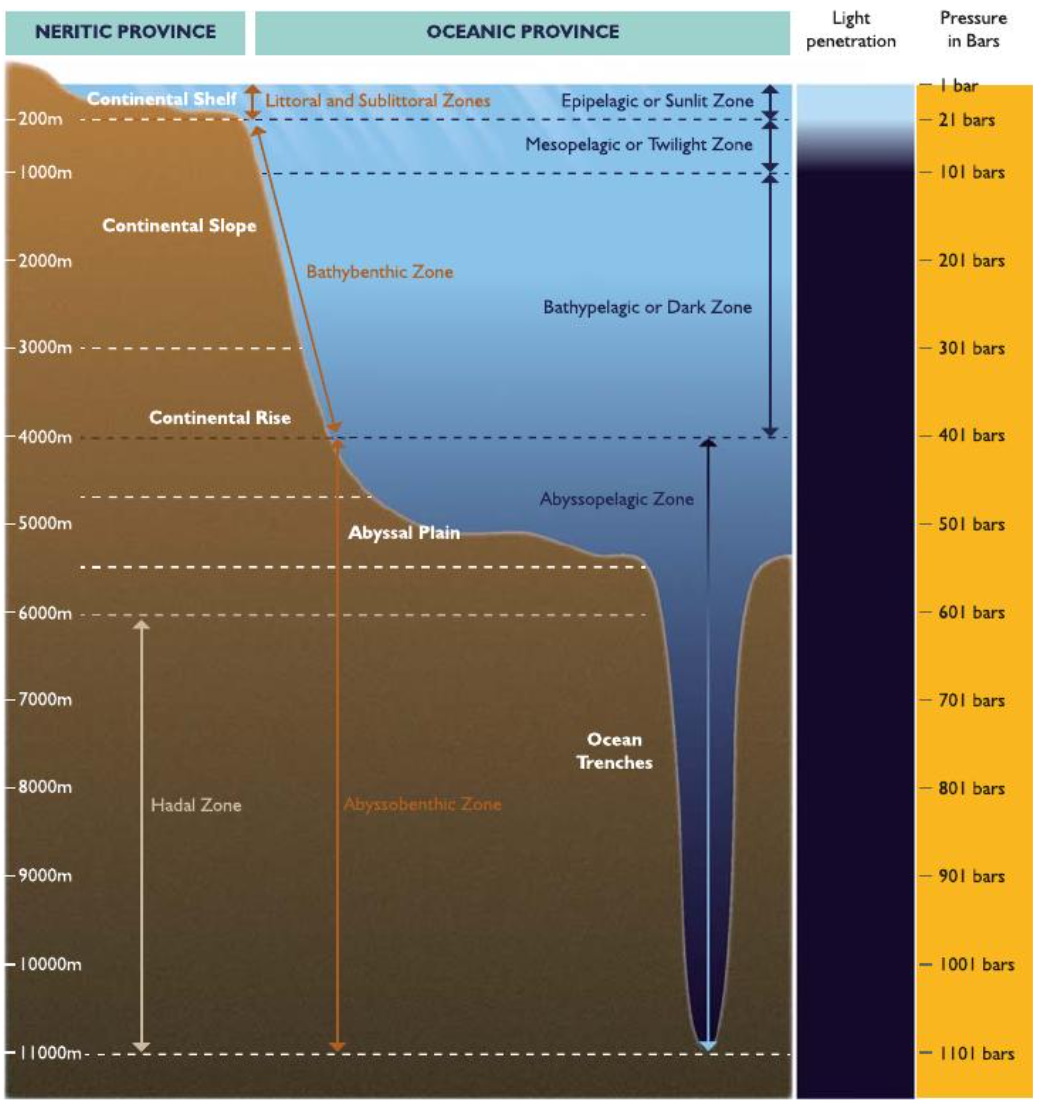
\includegraphics[width=0.4\textwidth]{images/01_intro/strat_vertical_el_marine_ecology}
		\caption{Stratification verticale de l'eau selon la pénétration de la lumière et de la pression, stratification horizontale selon la distance au plateau continental \cite{dipper2022}.}
		\label{fig:stratverticalelmarineecology}
	\end{figure}
	
	\section{Réponse fréquentielle des organismes pélagiques}
	\label{annexe:rep_freq}
		\begin{figure}[H]
			\centering
			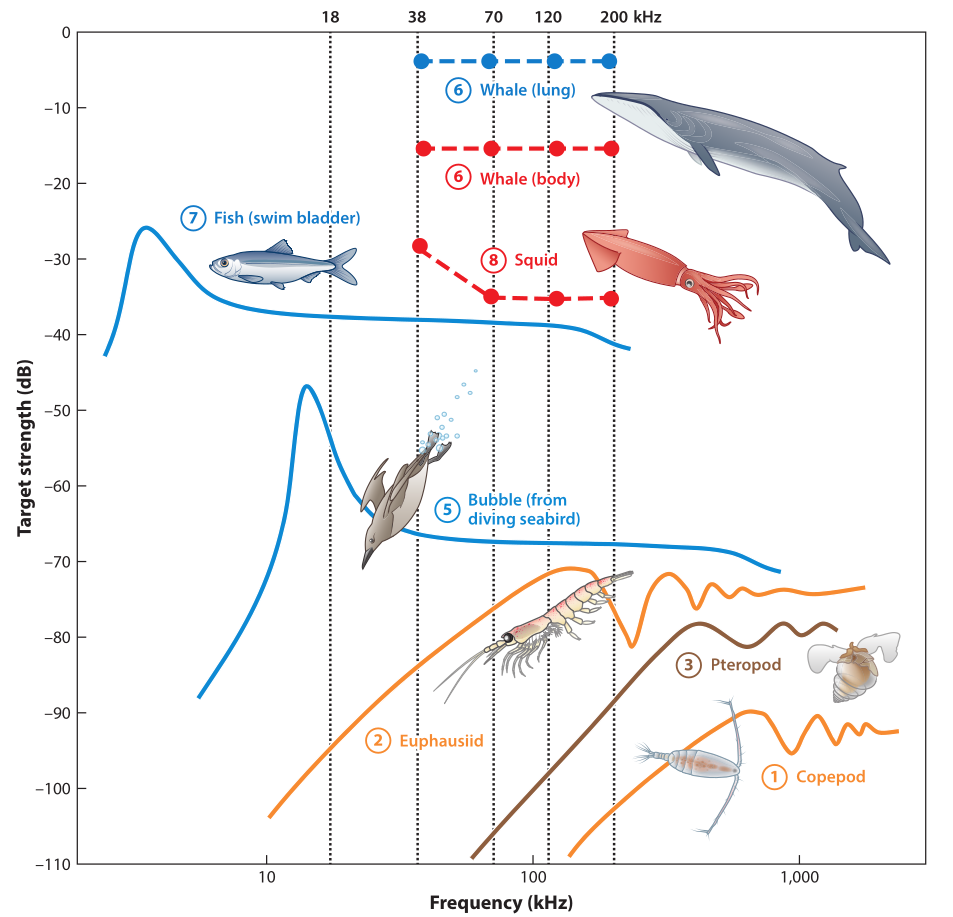
\includegraphics[width=0.5\textwidth]{images/05_annexes/02_materiel/freq_response_organisms_benoit_bird}
			\caption{Réponse fréquentielle des organismes pélagiques selon la fréquence de l'onde émise \cite{benoitbird2016ecological}}
			\label{fig:freqresponse}
		\end{figure}
		
	% Méthode
	% Préprocessing
	\section{Valeurs manquantes sur le volume de rétropropagation acoustique $S_v$ en fonction de la profondeur et de la fréquence de l'échosondeur}
	\label{annexe:missing_values}
		\begin{figure}[H]
			\centering
			
			\begin{subfigure}[b]{0.49\textwidth}
				\centering
				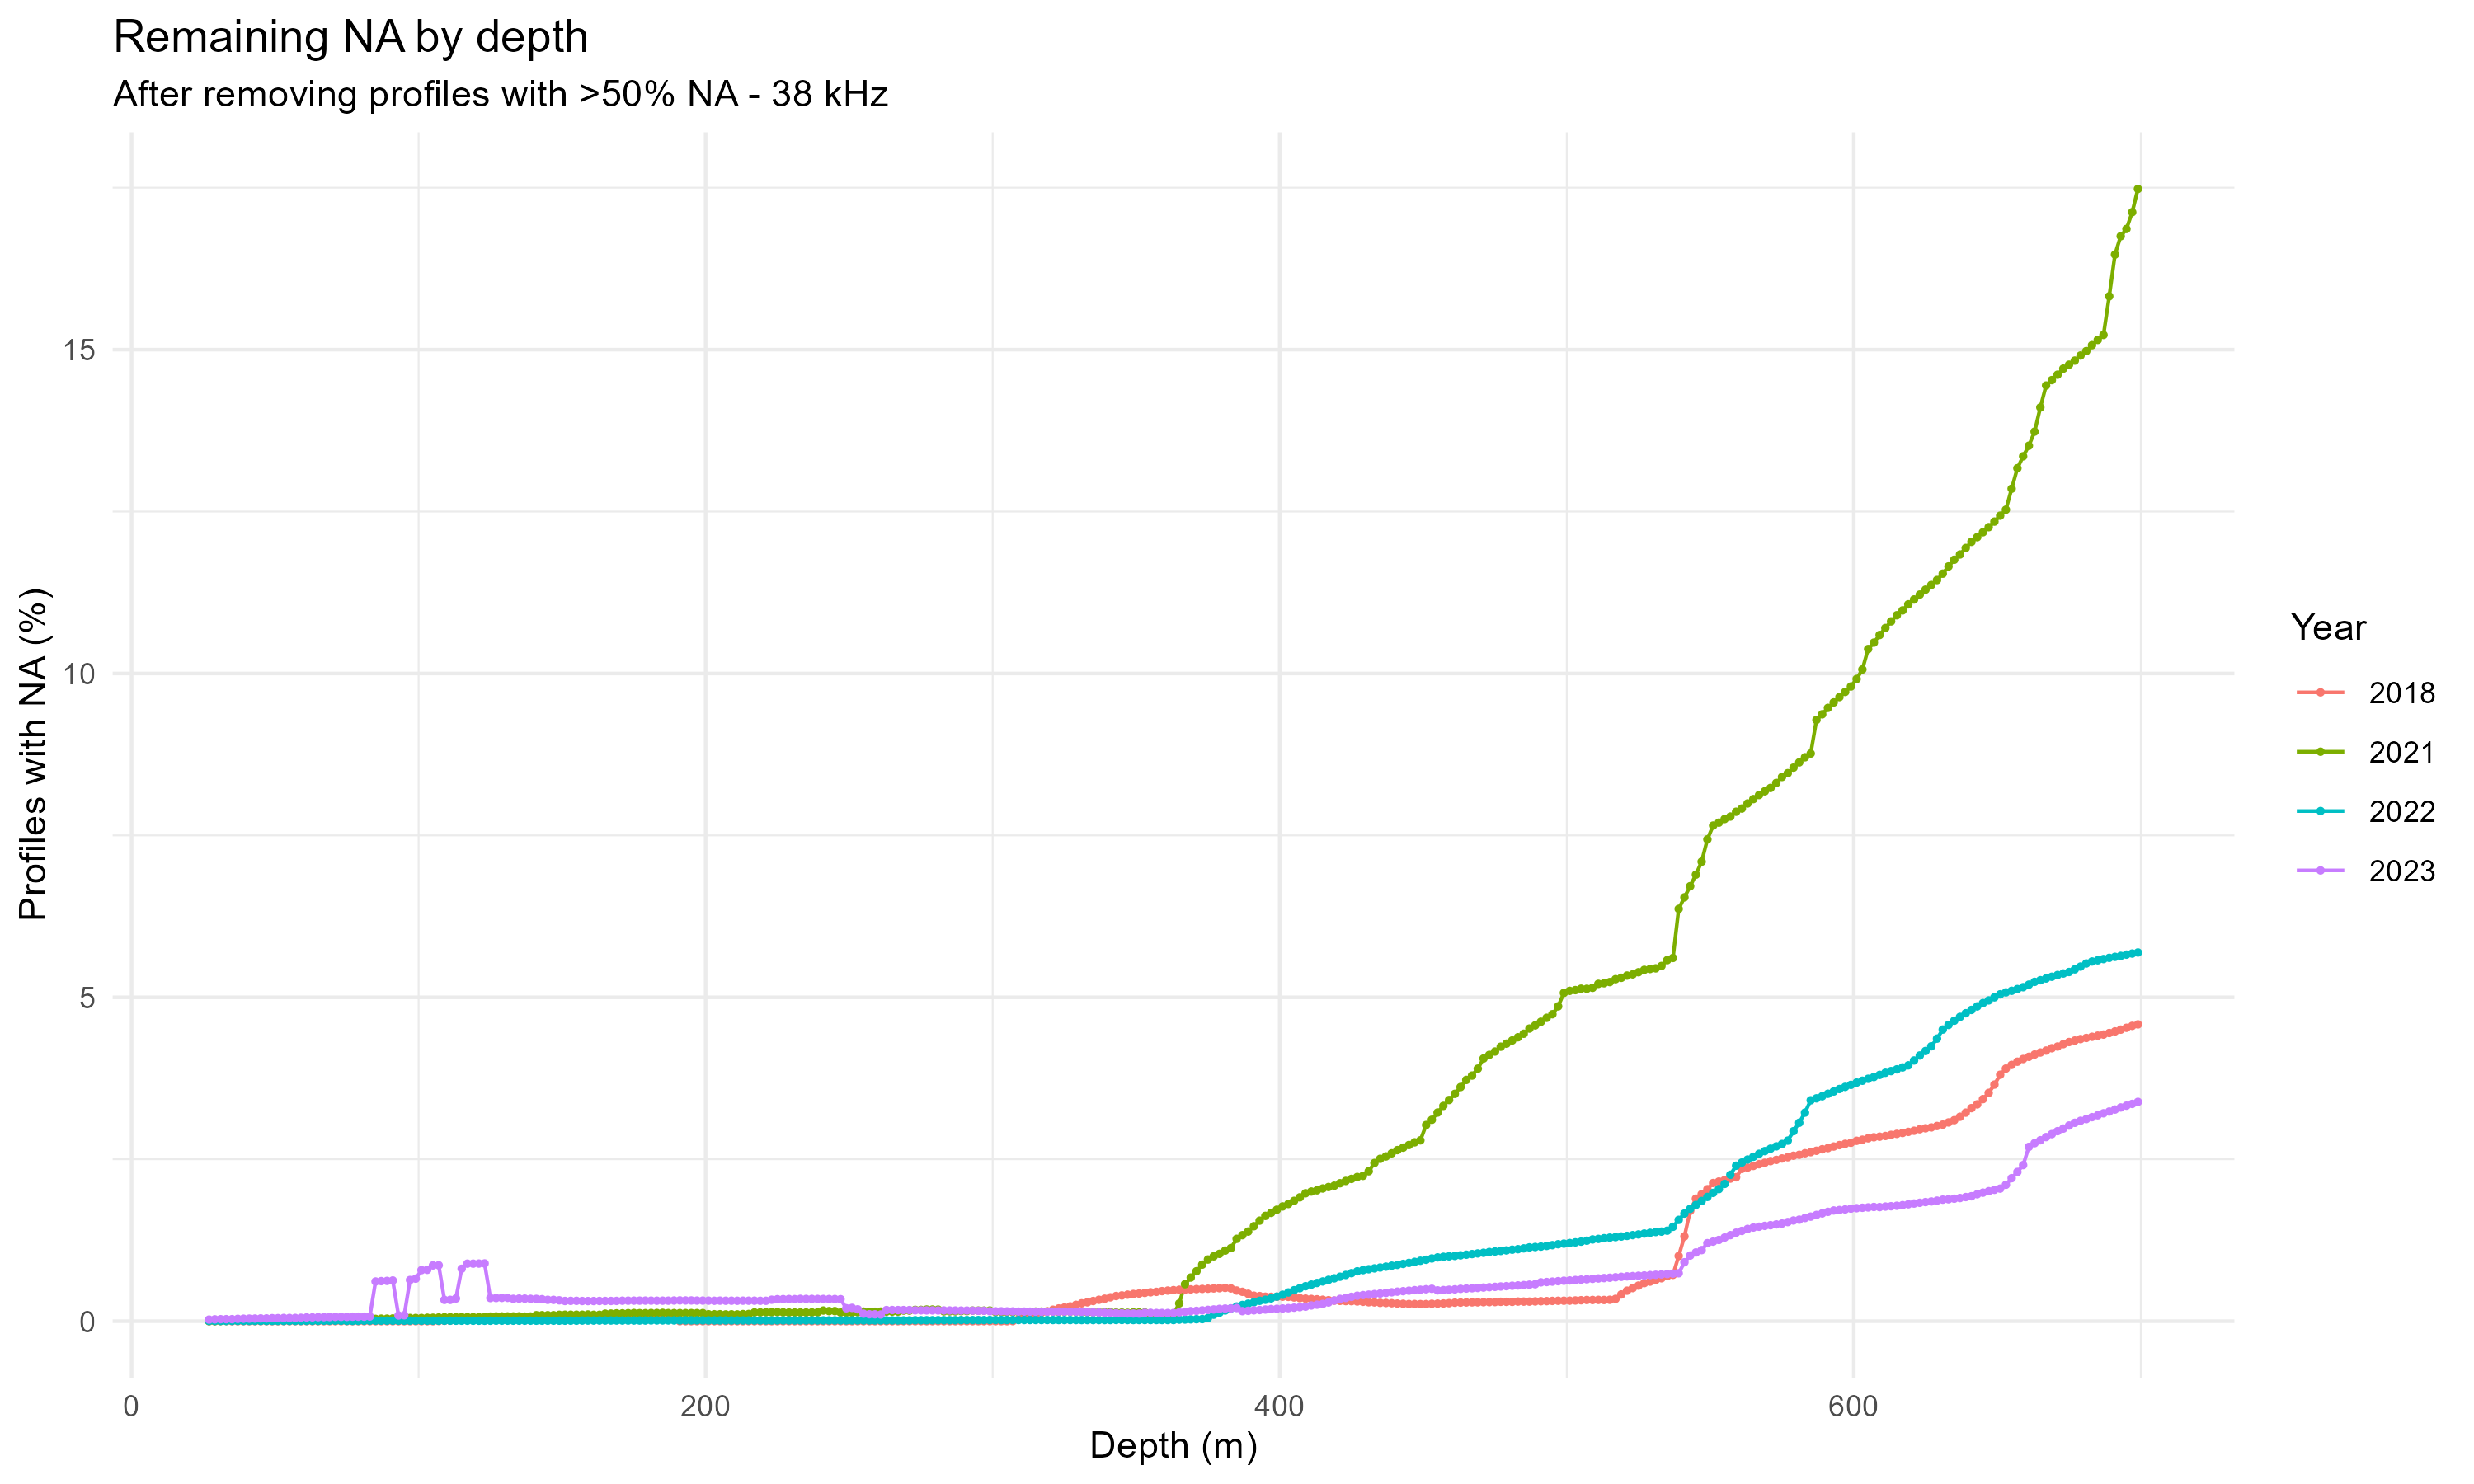
\includegraphics[width=\textwidth]{images/05_annexes/02_materiel/nasc_nas_per_depth/38kHz/diag_NA_by_depth_per_esu_38kHz}
				\caption{Fréquence de 38 kHz}
				\label{fig:diagnabydepthperesu38khz}
			\end{subfigure}
			\hfill
			\begin{subfigure}[b]{0.49\textwidth}
				\centering
				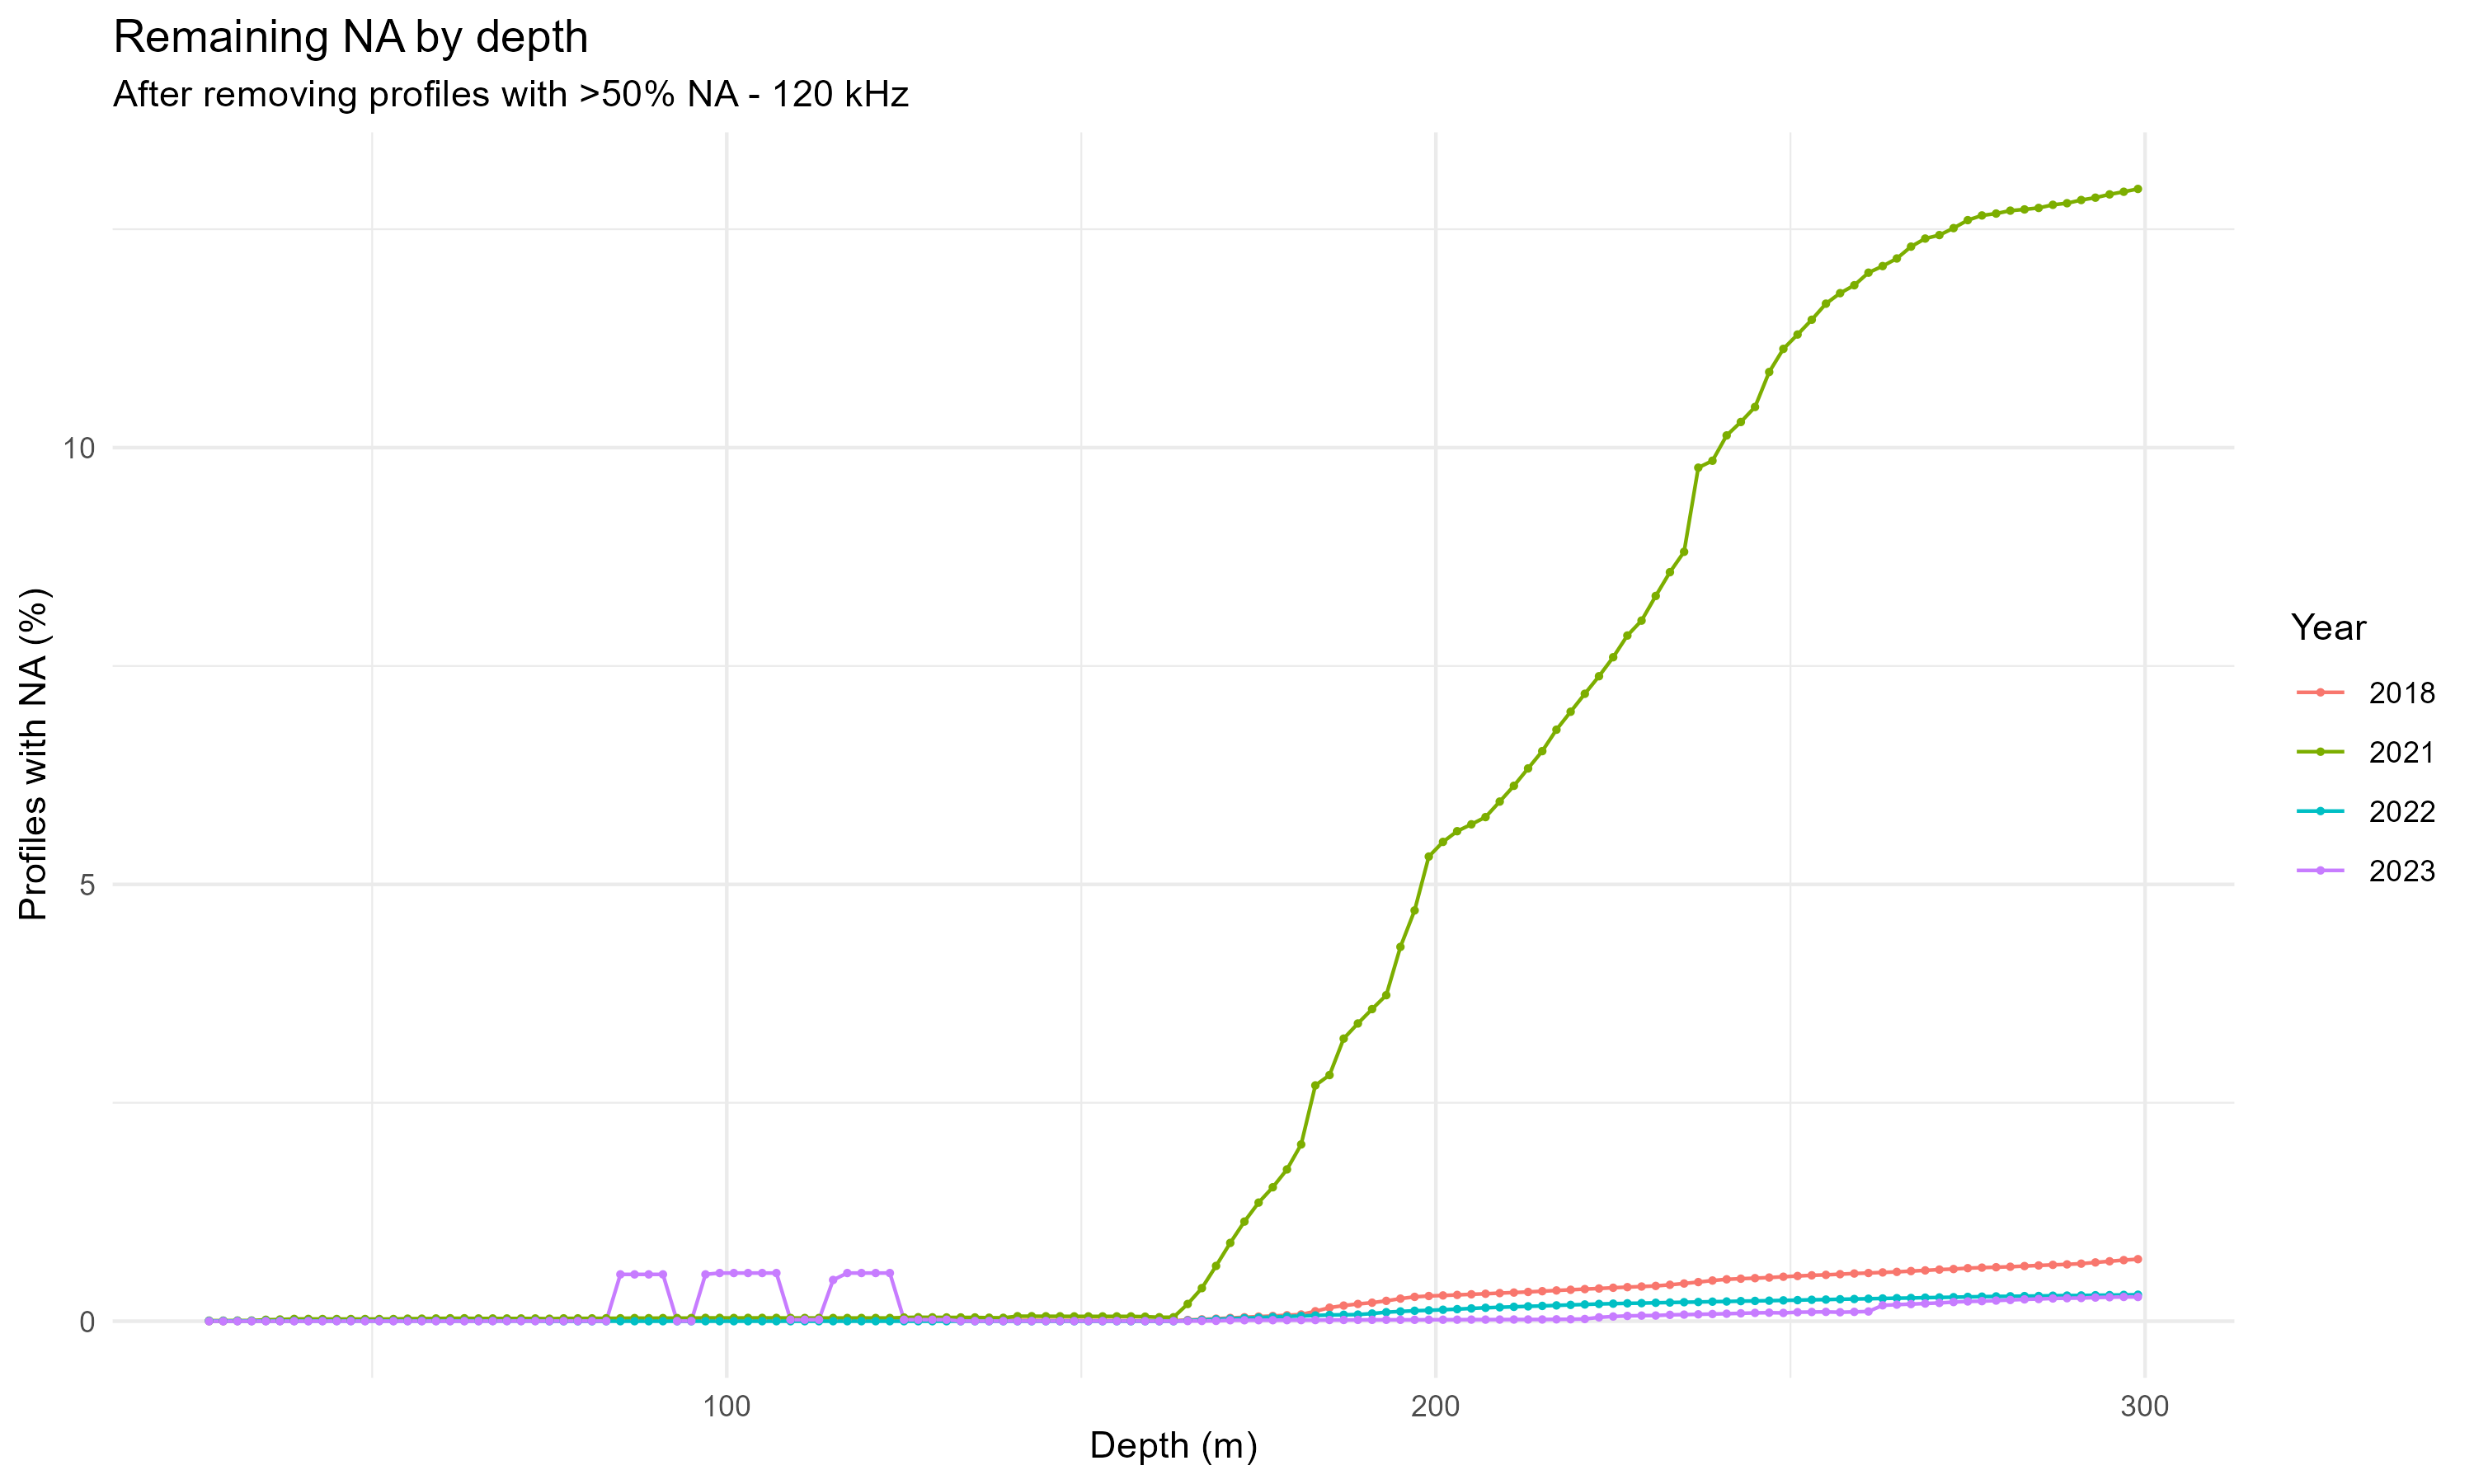
\includegraphics[width=\textwidth]{images/05_annexes/02_materiel/nasc_nas_per_depth/120kHz/diag_NA_by_depth_per_esu_120kHz}
				\caption{Fréquence de 120 kHz}
				\label{fig:diagnabydepthperesu120khz}
			\end{subfigure}
			
			\caption{Valeurs manquantes du coefficient de rétrodiffusion volumique $S_v$ en fonction de la profondeur, pour les fréquences de fonctionnement de l'échosondeur de 38 kHz et 120 kHz.}
			\label{fig:diagnabydepthperesu}
		\end{figure}
	
	\section{Méthode de calcul des FOD}
		\label{annexe:methode_fod}
		\subsection{Estimation par projection sur des bases de B-splines des profils de température et salinité}
		
			\subsubsection{Basis-splines de degré $m$ \cite{deBoor}}
			Les Basis-splines (B-splines) peuvent servir de base pour l'estimation par projection (estimation semi-paramétrique ou fonctionelle). Ce sont des fonctions à support local pouvant être définies par la récurrence de Cox-de-Boor \cite{deBoor} :
			\begin{figure}[H]
				\centering
				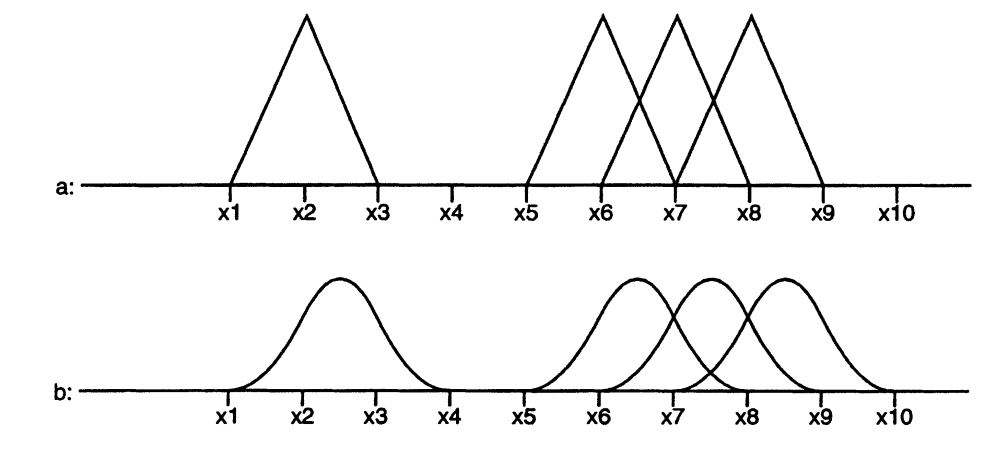
\includegraphics[width=0.6\textwidth]{images/03_methodology/b_splines_eilers}
				\caption{Illustration d'une B-spline isolée et de B-splines chevauchantes, de degré 1 (a) et de degré 2 (b) \cite{eilers1996}}
				\label{fig:bsplines}
			\end{figure}
			
			
			Soit $\phi_{i,m}(x)$ la B-spline de degré $m$ dont le support est $supp(\phi_{i,m}(x)) = [\tau_i, \tau_{i+m+1}]$. Avec $\tau_i, \ldots, \tau_{i+m+1}$ les noeuds (équi-espacés ou non). On peut définir la B-spline $\phi_{i,m}(x)$ comme suis \cite{deBoor} : 
			\begin{enumerate}
				\item Initialisation d'une fonction porte par noeud (degré 0, ordre 1)
				\begin{equation}
					\phi_{i,0}(x) = \begin{cases}
						1 & \text{si } \tau_i \leq x < \tau_{i+1} \\
						0 & \text{sinon}
					\end{cases}
				\end{equation}
				
				\item Réccurence : combinaison convexe de B-splines de degré inférieur à deux noeuds consécutifs
				\begin{equation}
					\phi_{i, m}(x) = \omega_{i,m}(x)\, \phi_{i, m-1}(x) + \big(1 - \omega_{i+1,m}(x)\big)\, \phi_{i+1, m-1}(x)
				\end{equation}
				avec
				\begin{equation}
					\omega_{j,m}(x) := \frac{x - \tau_j}{\tau_{j+m}- \tau_j}, \forall j
				\end{equation}
				(le poids de chaque terme est normalisé par le support de la B-spline de degré $m-1$ qu'il pondère : $\text{supp}(\phi_{i,m-1}) = [\tau_i, \tau_{i+m}]$ et $\text{supp}(\phi_{i+1,m-1}) = [\tau_{i+1}, \tau_{i+1+m}]$).
			\end{enumerate}
		
		
			\subsubsection{Espace des splines et base de B-splines}
				Soit $\tau = (\tau_1,\ldots,\tau_{2m+L+2})$ une suite de noeuds définie par
				\begin{equation} \underbrace{a = \tau_1 = \tau_2 = \cdots = \tau_{m+1}}_{m+1 \text{ noeuds répétés en } a} < \underbrace{\tau_{m+2} < \cdots < \tau_{m+L+1}}_{L \text{ noeuds intérieurs}} < \underbrace{\tau_{m+L+2} = \cdots = \tau_{2m+L+2}=b}_{m+1 \text{ noeuds répétés en } b} \end{equation}
				
				On note $\mathbb{S}_{m,\tau}$ l'espace des fonctions splines de degré $m$ associées à cette suite de noeuds. Une spline $f\in\mathbb{S}_{m,\tau}$ est une fonction polynomiale par morceaux de degré au plus $m$, définie sur les intervalles délimités par les noeuds $\tau$, et satisfaisant les conditions de continuité imposées par les multiplicités des noeuds \footnote{\begin{itemize}
						\item Continuité : $\phi_{i, m}(x) \in C^{m-1}$ aux noeuds. Pour une B-spline cubique ($m=3$), $\phi_{i, 3} \in \mathcal{C}^{2}$,
						\item Support compact : $\text{supp}(\phi_{i,m}) = [\tau_i, \tau_{i+m+1}]$, 
						donc $\langle \phi_{i,m}, \phi_{j,m} \rangle = 0$ si $|i-j| \geq m+1$.
						\item Positivité : $\phi_{i,m}(x) > 0$ sur $(\tau_i, \tau_{i+m+1})$ 
						et $\phi_{i,m}(x) = 0$ sinon.
				\end{itemize}}.
				
				Les B-splines de degré $m$ associées à la suite de noeuds $\tau$, notées $\{\phi_{i,m}\}_{i=1}^{L+m+1}$	constituent une base de l'espace $\mathbb{S}_{m,\tau}$ ($\dim(\mathbb{S}_{m,\tau})=L+m+1$).
				
				Par conséquent, toute fonction spline $f\in\mathbb{S}_{m,\tau}$ peut s'écrire de manière unique comme une combinaison linéaire des B-splines :
				\begin{equation}
					\boxed{
						f(x)=\sum_{i=1}^{L+m+1}\alpha_i\phi_{i,m}(x),
						\qquad \alpha_i\in\mathbb{R}.
					}
				\end{equation}
				
				\subsubsection{Estimation fonctionnelle par minimisation des moindres carrés pénalisée (O-Splines) \cite{wand2008}, \cite{eilers1996}}
				\label{par:moindres_carres}
				
				Appliquons maintenant ce cadre à l'estimation fonctionnelle des profils de température et de salinité. Soit $l$ un indice spatio-temporel (combinaison d'un instant, d'une longitude et d'une latitude) et $v \in {T,S}$ la variable considérée. Le profil brut $\mathbf{v}_l \in \mathbb{R}^{n_{depths}}$ correspond aux valeurs de $v$ issues du modèle Copernicus aux profondeurs discrètes $z_1,\ldots,z_{n_{depths}}$. On suppose que ces observations proviennent de l'évaluation d'une fonction sous-jacente $f_l$ aux profondeurs considérées :
				\begin{equation}
					v_l(z_k)=f_l(z_k)+\varepsilon_k,
					\qquad k=1,\ldots,n_{depths},
				\end{equation}
				où $\varepsilon_k$ représente le terme d'erreur associé à l'observation du profil à la profondeur $z_k$.
				
				L'objectif est d'estimer $f_l$ sur l'intervalle de profondeur $[a,b]$, qui correspond ici à $[20,500]$ m. On cherche pour cela une approximation $\hat f_l \in \mathbb{S}_{m,\tau}$ sous la forme d'une combinaison linéaire des B-splines définies précédemment :
				\begin{equation}
					\hat f_l(z)
					=
					\sum_{i=1}^{K}
					\alpha_{l,i}\,\phi_{i,m}(z),
					\qquad K=L+m+1.
				\end{equation}
				où $L$ désigne le nombre de noeuds intérieurs et $K$ le nombre total de B-splines. Les coefficients $\boldsymbol{\alpha}_l = (\alpha_{l,1},\ldots,\alpha_{l,K})^\top$ déterminent ainsi entièrement la spline estimée pour le profil $l$. Pour un profil donné, les coefficients $\boldsymbol{\alpha}_l$ sont déterminés en minimisant l'erreur d'ajustement entre les observations et la spline. La fonction objectif des moindres carrés est
				\begin{align}
					S_l
					&=
					\sum_{k=1}^{n_{depths}}
					\left(
					v_l(z_k)-\hat f_l(z_k)
					\right)^2
					\\
					&=
					\sum_{k=1}^{n_{depths}}
					\left(
					v_l(z_k)
					-
					\sum_{i=1}^{K}
					\alpha_{l,i}\phi_{i,m}(z_k)
					\right)^2.
				\end{align}
				
				Cependant, lorsque le nombre de noeuds est élevé, l'ajustement peut devenir excessivement flexible et conduire à un sur-ajustement (\textit{overfitting}). Afin de contrôler la complexité de la fonction estimée, on introduit une pénalisation de sa rugosité\footnote{mesure le degré d'irrégularité d'une fonction, est quantifié par l'intégrale du carré de sa dérivée seconde}. La matrice de pénalisation $\Omega$ est définie par
				\begin{equation}
					\Omega_{i,j}
					=
					\int_a^b
					\phi_{i,m}''(z)\phi_{j,m}''(z)\,\mathrm{d}z,
					\qquad
					1\leq i,j\leq K.
				\end{equation}
				
				Le critère pénalisé à minimiser pour le profil $l$ est alors
				\begin{equation}
					S_{l,\lambda}
					=
					\underbrace{
						\sum_{k=1}^{n_{depths}}
						\left(
						v_l(z_k)
						-
						\sum_{i=1}^{K}
						\alpha_{l,i}\phi_{i,m}(z_k)
						\right)^2
					}_{\text{erreur d'ajustement}}
					+
					\lambda
					\underbrace{
						\boldsymbol{\alpha}_l^\top
						\Omega
						\boldsymbol{\alpha}_l
					}_{\text{pénalisation de la rugosité}}.
				\end{equation}
				où $\lambda\geq0$ est le paramètre de lissage contrôlant le compromis entre fidélité aux observations et régularité de la fonction estimée.
				Dans notre cas, le nombre de splines $K$ et le paramètre de lissage $\lambda$ ont été choisi par validation croisée leave-one-out (CV-LOO). On trouve $\lambda = 0.25$ pour $K = 25$ splines
				
				\begin{figure}[h]
					\centering
					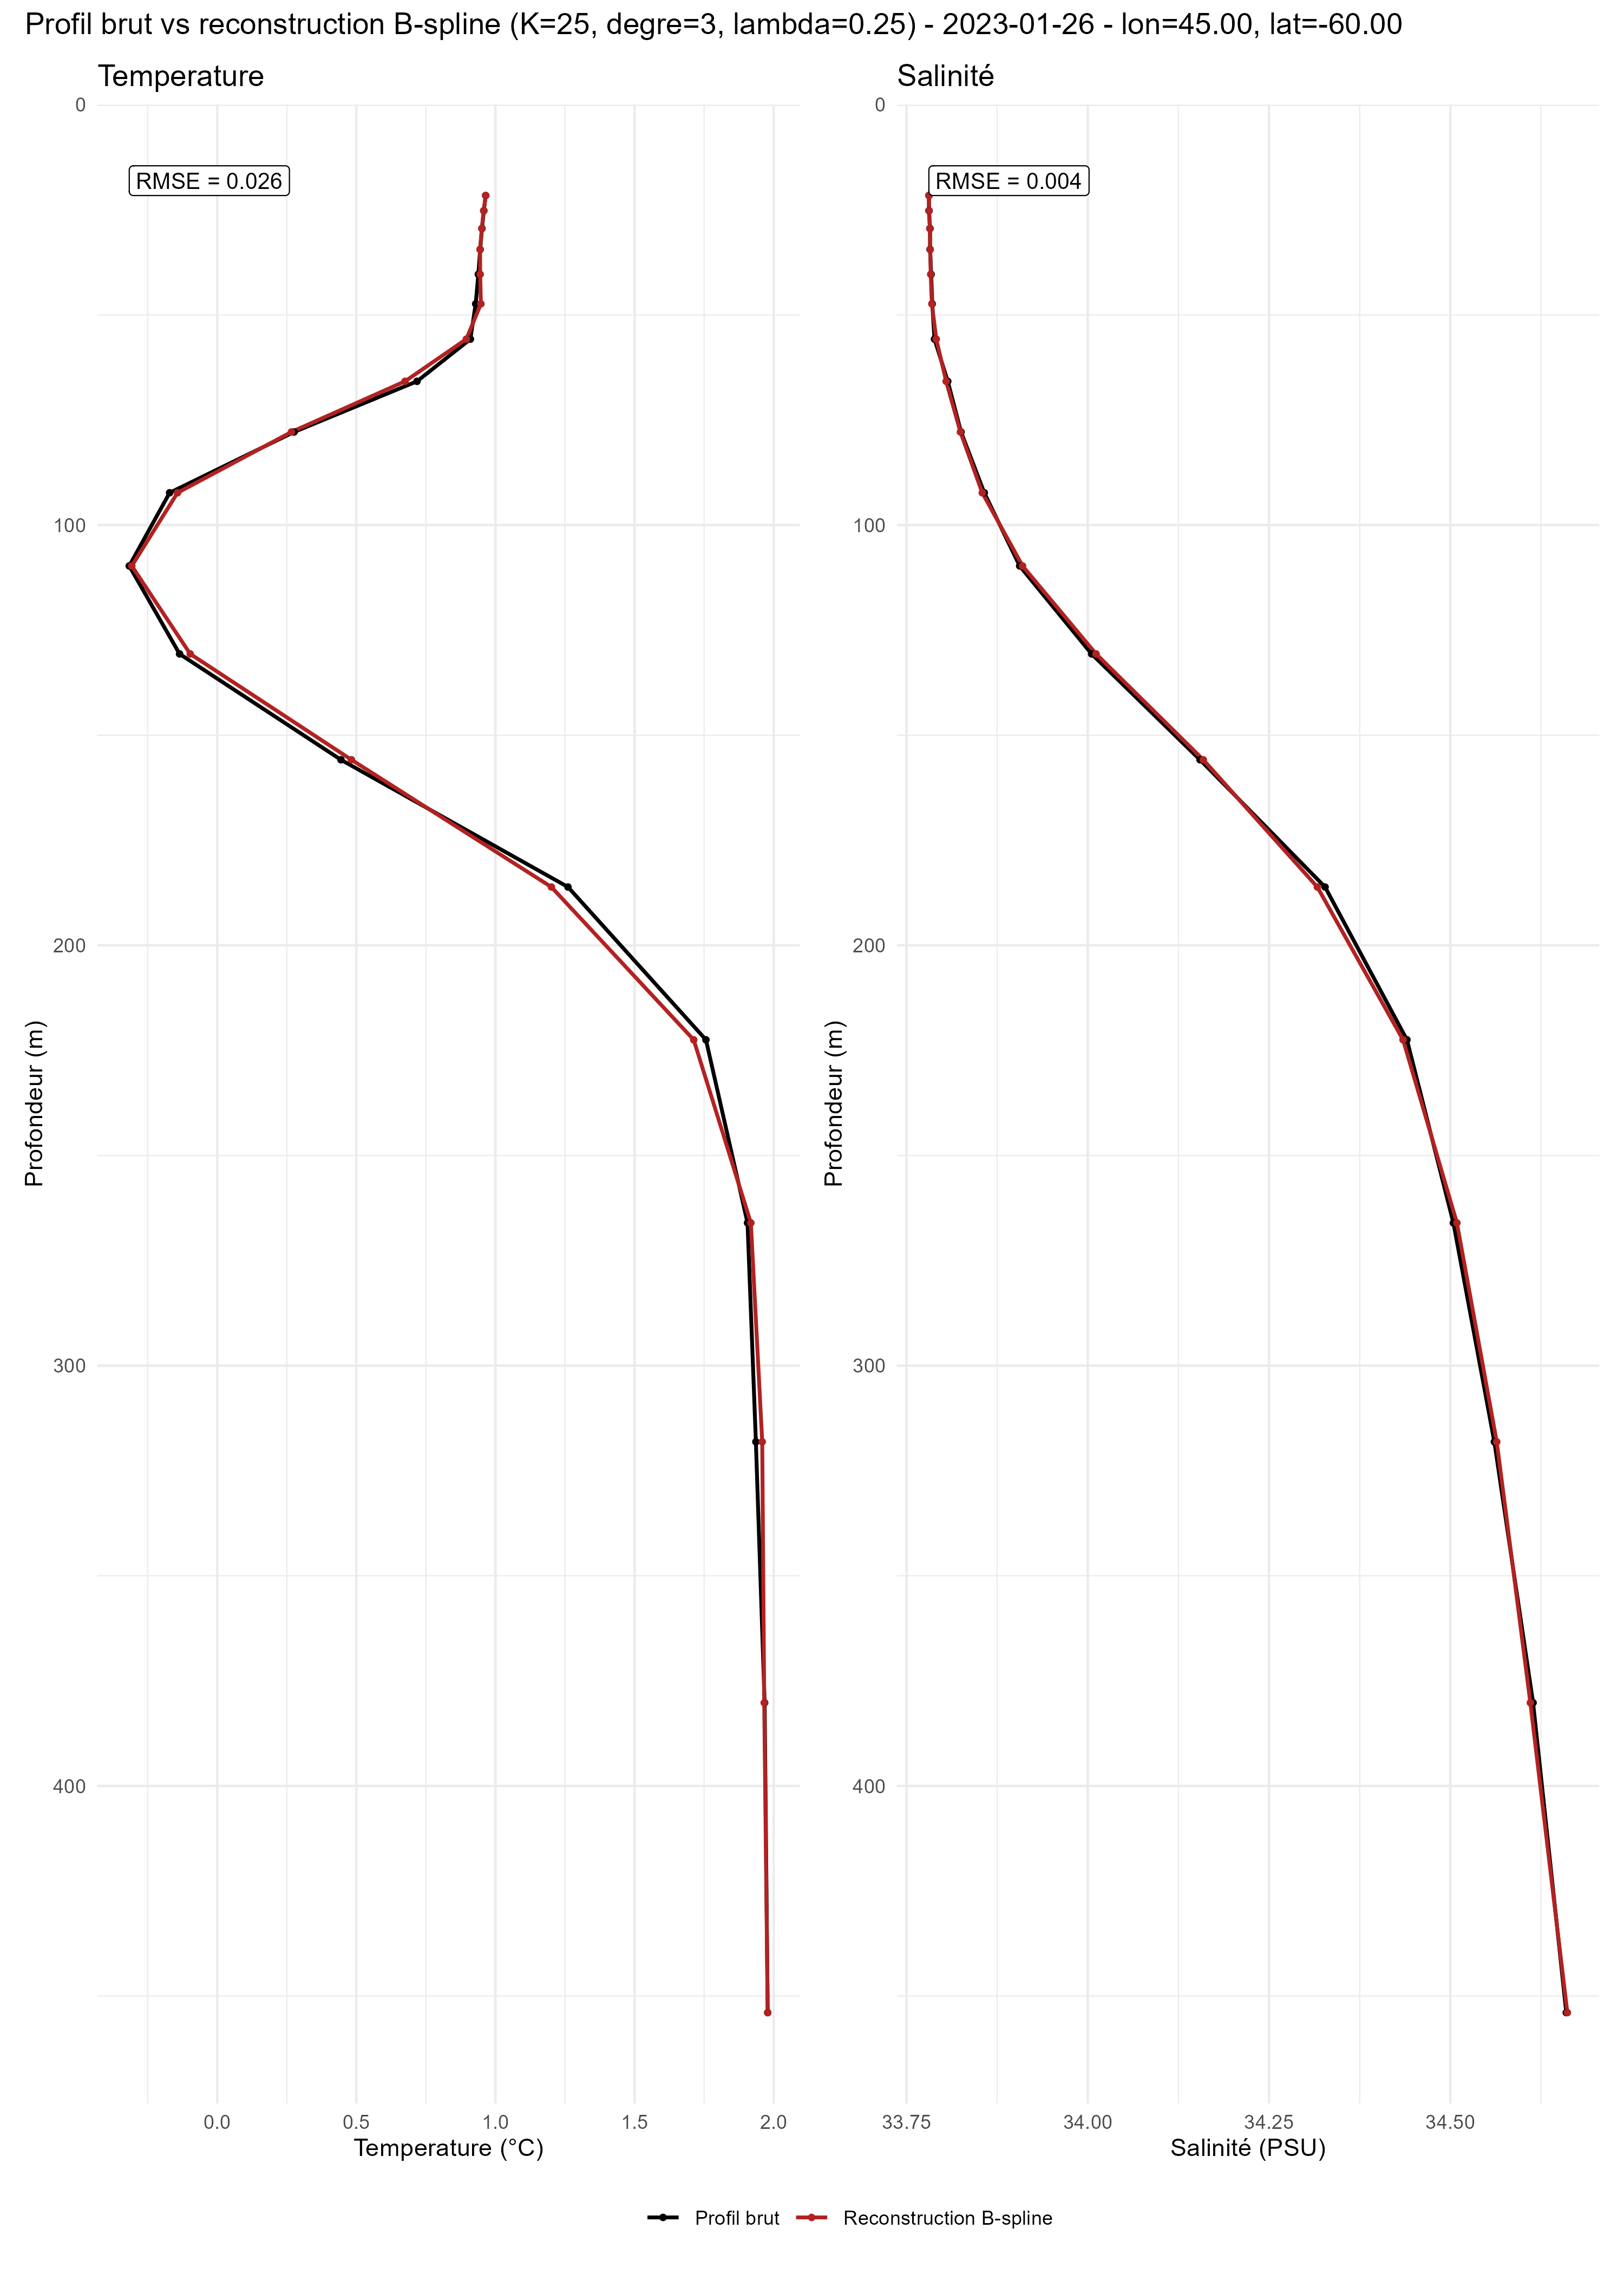
\includegraphics[width=0.5\textwidth]{images/03_methodology/profil_bspline_temp_sal_lon45.00_lat-60.00}
					\caption[]{Estimation fonctionelle des profils de Température/Salinité ($\lambda = 0.25, K=25$) issu de Copernicus (E.U. Copernicus Marine Service Information (CMEMS). Global Ocean Physics Reanalysis. Marine Data Store (MDS). DOI: 10.48670/moi-00021) le 2023-01-26 aux coordonnées 450E,-60°N.}
					\label{fig:profilbsplinetempsal}
				\end{figure}
		
		\subsection{Réduction de dimension par Analyse en Composante Principale}
		
			Suite à l'estimation fonctionnelle réalisée à l'étape précédente, chaque profil $l$ est désormais représenté par un couple de fonctions de la profondeur, la température et la salinité, estimées sur la même base de B-splines $(\Phi_k)_{1\leq k \leq K}$ définie sur $[d_{min}, d_{max}]$ :
			\[
			T_l(z) = \sum_{k=1}^{K} \alpha_{l,k}^{T}\, \Phi_k(z), 
			\qquad
			S_l(z) = \sum_{k=1}^{K} \alpha_{l,k}^{S}\, \Phi_k(z),
			\qquad z \in [d_{min}, d_{max}]
			\]
			On considère alors chaque profil comme une observation \textbf{bivariée} $X_l = (T_l, S_l) \in \big(L^2([d_{min}, d_{max}])\big)^2$, muni du produit scalaire
			\[
			\langle (f_1, g_1), (f_2, g_2) \rangle = \langle f_1, f_2 \rangle_{L^2} + \langle g_1, g_2 \rangle_{L^2}
			\]
			L'objectif de cette étape est de réduire conjointement la dimension des profils de température et de salinité, afin de capturer les modes de variabilité communs aux deux variables.
			
			Une approche pour réduire la dimension des données est l'analyse par composante principale (ACP ou PCA pour Principal Component Analysis). Puisque les données sont dans un espace fonctionnel $\mathbb{S}_{m,\tau}$, on parle alors d'Analyse par Composante Principale \textit{fonctionnelle} (ACPf ou FPCA). La logique est identique à celle d'une PCA classique mais les outils sont adaptés pour manipuler les fonctions. Ici, la fPCA est réalisée conjointement sur les deux variables, on parle de fPCA bivariée.
			
			\subsubsection{Construction du vecteur de coefficients bivarié}
				Pour chaque profil $l$, on concatène les coefficients de B-spline de température et de salinité en un unique vecteur $\alpha_l \in \mathbb{R}^{2K}$ :
				\[
				\alpha_l = \begin{pmatrix} \alpha_l^{T} \\ \alpha_l^{S} \end{pmatrix}, 
				\qquad \alpha_l^{T} = (\alpha_{l,1}^T, \ldots, \alpha_{l,K}^T)^\top, 
				\quad \alpha_l^{S} = (\alpha_{l,1}^S, \ldots, \alpha_{l,K}^S)^\top
				\]
				En empilant les $N$ profils, on obtient la matrice $\alpha \in \mathbb{R}^{N \times 2K}$.
		
			\subsubsection{Centrage des données}
				Soit $\overline{\alpha} \in \mathbb{R}^{2K}$ la moyenne empirique, sur l'ensemble des $N$ profils, des coefficients de chaque B-spline pour la partie température et pour la partie salinité :
				\[
				\overline{\alpha} = \frac{1}{N} \sum_{l=1}^{N} \alpha_l
				\]
				
				On obtient ainsi les coefficients bivariés centrés $\tilde{\alpha} =  \alpha_{l} - \overline{\alpha}$, avec $\tilde{\alpha} \in \mathbb{R}^{N \times 2K}$. Pour $l \in N$ : 
				$$
				\tilde\alpha_l
				=
				\begin{pmatrix}
					\tilde\alpha_l^T\\
					\tilde\alpha_l^S
				\end{pmatrix}
				\in\mathbb{R}^{2K}
				$$
		
			\subsubsection{Calcul de la covariance empirique}
		
				On définit la matrice bivariée de fonctions de base $\boldsymbol{\Phi}(z) \in \mathbb{R}^{2\times 2K}$ comme la concaténation de la base $\Phi$ utilisée pour chacune des deux composantes :
				
				$$
				\boldsymbol{\Phi}(z)
				=
				\begin{pmatrix}
					\Phi(z)^\top & 0\\
					0 & \Phi(z)^\top
				\end{pmatrix}
				\in\mathbb{R}^{2\times 2K},
				$$
				
				de sorte que le profil bivarié centré s'écrive $
				\tilde X_l(z)
				=
				\boldsymbol{\Phi}(z)\tilde\alpha_l
				=
				\begin{pmatrix}
					\tilde T_l(z)\\
					\tilde S_l(z)
				\end{pmatrix}.
				$
				
				La covariance empirique entre deux profondeurs $s$ et $t$ est alors une matrice $2\times2$ donnée par
				
				$$
				\hat V(s,t)
				=
				\frac{1}{N}
				\sum_{l=1}^N
				\tilde X_l(s)\tilde X_l(t)^\top.
				$$
				
				En introduisant la matrice de covariance empirique des coefficients
				
				$$
				C
				=
				\frac{1}{N}\tilde\alpha^\top\tilde\alpha
				\in\mathbb{R}^{2K\times2K},
				$$
				
				on obtient
				
				$$
				\boxed{
					\hat V(s,t)
					=
					\boldsymbol{\Phi}(s)\,
					C\,
					\boldsymbol{\Phi}(t)^\top.
				}
				$$
				
				Cette matrice contient à la fois les covariances intra-variables, correspondant aux blocs température--température et salinité--salinité, et les covariances croisées température--salinité.
		
			\subsubsection{Décomposition en valeurs propres et vecteurs propres de la matrice de covariance}
		
				On effectue la décomposition spectrale de l'opérateur de covariance $\hat{V}$ :
				\[
				\int \hat{V}(s, t)\,\xi(t)\, dt = \rho\, \xi(s)
				\]
				avec la contrainte d'orthonormalité des fonctions propres bivariées : $\|\xi\|_{L^2} = 1$ et $\langle \xi_i, \xi_j\rangle = 0$ si $i \neq j$.
				
				On fait l'hypothèse que la fonction propre bivariée $\xi(t)$ se décompose dans la même base bivariée que nos profils :
				\[
				\xi(t) = \boldsymbol{\Phi}^\top(t)\, b, \qquad b \in \mathbb{R}^{2K}
				\]
				
				On a alors :
				\begin{align*}
					\int \hat{V}(s, t)\,\xi(t)\,dt 
					&= \int \frac{1}{N} \boldsymbol{\Phi}^\top(s)\tilde{\alpha}^\top \tilde{\alpha}\, \boldsymbol{\Phi}(t)\, \boldsymbol{\Phi}^\top(t)\, b\,dt \\
					&= \frac{1}{N} \boldsymbol{\Phi}^\top(s)\tilde{\alpha}^\top \tilde{\alpha} 
					\underbrace{\int \boldsymbol{\Phi}(t)\boldsymbol{\Phi}^\top(t)\,dt}_{=\, W} \, b \\
					&= \frac{1}{N}\boldsymbol{\Phi}^\top(s)\,\tilde{\alpha}^\top \tilde{\alpha}\, W\, b
				\end{align*}
				où $W = \int \boldsymbol{\Phi}(t)\boldsymbol{\Phi}^\top(t)\,dt \in \mathbb{R}^{2K \times 2K}$ est la matrice de Gram de la base bivariée. Comme $\boldsymbol{\Phi}(t)$ répète deux fois la même base $\Phi(t)$, $W$ prend la forme bloc-diagonale
				\[
				W = \begin{pmatrix} W_0 & 0 \\ 0 & W_0 \end{pmatrix}, 
				\qquad W_0 = \int \Phi(t)\Phi^\top(t)\,dt \in \mathbb{R}^{K \times K}
				\]
				les blocs hors-diagonale étant nuls car la partie température et la partie salinité de $\xi$ n'interagissent qu'au travers de la covariance des coefficients $\tilde\alpha^\top\tilde\alpha$, pas au travers de la base elle-même.
				
				On peut donc réécrire la décomposition spectrale comme suit :
				\begin{align*}
					& \int \hat{V}(s, t)\,\xi(t)\,dt = \rho\, \xi(s)\\
					& \iff \frac{1}{N}\boldsymbol{\Phi}^\top(s)\,\tilde{\alpha}^\top \tilde{\alpha}\, W\, b = \rho\, \boldsymbol{\Phi}^\top(s)\, b\\
					& \iff \frac{1}{N} \tilde{\alpha}^\top \tilde{\alpha}\, W\, b = \rho\, b
				\end{align*}
				
				La matrice $\tilde\alpha^\top\tilde\alpha$ est symétrique (c'est un produit de la forme $A^\top A$), mais le produit $\tilde\alpha^\top\tilde\alpha\, W$ ne l'est pas en général : le problème aux valeurs propres n'est donc pas directement résoluble par une décomposition spectrale standard. Pour contourner ce problème, on utilise le changement de variable $b = W^{-\frac{1}{2}} u$ :
				\begin{align*}
					& \frac 1 N \tilde{\alpha}^\top \tilde{\alpha}\, W\, b = \rho\, b\\
					& \iff \frac 1 N \tilde{\alpha}^\top \tilde{\alpha}\, W\, W^{-\frac 1 2}u = \rho\, W^{-\frac 1 2}u\\
					& \iff \frac 1 N \tilde{\alpha}^\top \tilde{\alpha}\, W^{\frac{1}{2}} u = \rho\, W^{-\frac{1}{2}} u \\
					& \iff \frac 1 N \underbrace{W^{\frac 1 2}\, \tilde{\alpha}^\top \tilde{\alpha}\, W^{\frac 1 2}}_{\text{symétrique}}\, u = \rho\, u
				\end{align*}
				La matrice $W^{1/2}\tilde\alpha^\top\tilde\alpha\, W^{1/2}$ est bien symétrique (elle est de la forme $M^\top M$ avec $M = \tilde\alpha W^{1/2}$), ce qui garantit des valeurs propres réelles $\rho$ et des vecteurs propres $u$ orthogonaux. Une fois $u$ obtenu, on retrouve $b = W^{-1/2} u$, puis la fonction propre bivariée $\xi(t) = \boldsymbol{\Phi}^\top(t)\, b$, dont les deux moitiés de $b$ (les $K$ premiers et les $K$ derniers coefficients) donnent respectivement la composante "température" $\xi^T$ et la composante "salinité" $\xi^S$ de la fonction propre.
		
			\subsubsection{ Calcul des scores (projections), reconstruction dans l'espace propre et variance expliquée}
				Une fois les fonctions propres bivariées $\xi_j = (\xi_j^T, \xi_j^S)$ et valeurs propres $\rho_j$ calculées, on peut calculer les projections $c_{l,j}$ des profils bivariés centrés $\tilde X_l = (\tilde T_l, \tilde S_l)$ sur l'espace propre. On note $c_{l,j}$ le score du profil $l$ sur la $j$-ème composante principale (commun à la température et à la salinité, puisque la composante principale est bivariée) :
				\begin{align*}
					c_{l, j} &= \langle \tilde X_l, \xi_j\rangle \\
					&= \int \tilde\alpha_l^\top \boldsymbol{\Phi}(t)\, \boldsymbol{\Phi}^\top(t)\, b_j \, dt \\ 
					&= \tilde \alpha_l^\top\, W\, b_j \;\in \mathbb{R}
				\end{align*}
				
				On choisit ensuite $J \ll 2K$ composantes à partir de la variance expliquée cumulée. La variance expliquée cumulée des $J$ premières composantes principales est calculée comme suit :
				\[
				VE = \frac{\sum_{j=1}^{J}\rho_j}{\sum_{k=1}^{2K} \rho_k}	
				\]
				avec $\rho_k$ la valeur propre associée à la $k$-ième composante principale, les composantes étant triées par ordre \textbf{décroissant} de valeur propre ($\rho_1 \geq \rho_2 \geq \cdots$), de sorte que les $J$ premières composantes soient celles qui expliquent le plus de variance conjointe des profils de température et de salinité. On peut ainsi sélectionner par exemple les $J$ premières composantes principales qui expliquent $>99$\% de la variance. Dans notre cas nous avons choisis de conservées $J=6$ composantes principales qui expliquent $>99$\% explained var et permettent d'encoder assez correctement la variabilité des profils (il y a un compromis entre qualité de l'approximation et coût computationnel, ce pourquoi nous nous sommes limités à 6 PC, et non 10, malgré la qualité supérieure de reconstruction), voir figure \ref{fig:profilpcatempsalcompare}.
				
				\begin{table}[H]
					\centering
					\begin{tabular}{ccccc}
						\toprule
						PC & Eigenvalue & Prop. variance & Cumulative variance \\
						\midrule
						1  & 981.66665873 & 0.9810935 & 0.9810935 \\
						2  & 12.52661452  & 0.0125193 & 0.9936128 \\
						3  & 4.16020812   & 0.0041578 & 0.9977705 \\
						4  & 0.92707153   & 0.0009265 & 0.9986971 \\
						5  & 0.56820781   & 0.0005679 & 0.9992649 \\
						6  & 0.41429271   & 0.0004141 & 0.9996790 \\
						7  & 0.13458956   & 0.0001345 & 0.9998135 \\
						8  & 0.05806269   & 0.0000580 & 0.9998715 \\
						9  & 0.05427009   & 0.0000542 & 0.9999258 \\
						10 & 0.02370249   & 0.0000237 & 0.9999495 \\
						\bottomrule
					\end{tabular}
					\caption{Valeurs propres et variance expliquée par les composantes principales.}
					\label{tab:pca_variance}
				\end{table}
				
				\vspace{1em}
				
				Finalement, on peut reconstruire conjointement les profils de température et de salinité du profil $l$ comme la combinaison linéaire des $J$ premières fonctions propres bivariées et des scores associés (les mêmes scores $c_{l,j}$ pilotant simultanément la reconstruction des deux variables) :
				\[
				T_l(t) = \overline{T}(t) + \sum_{j=1}^{J} c_{l,j}\, \xi_j^T(t), 
				\qquad
				S_l(t) = \overline{S}(t) + \sum_{j=1}^{J} c_{l,j}\, \xi_j^S(t)
				\]
				où $\overline{T}$ et $\overline{S}$ sont les profils moyens de température et de salinité, obtenus à partir des composantes correspondantes de $\overline\alpha$.
				
				\begin{figure}[H]
					\centering
					
					\begin{subfigure}{0.3\textwidth}
						\centering
						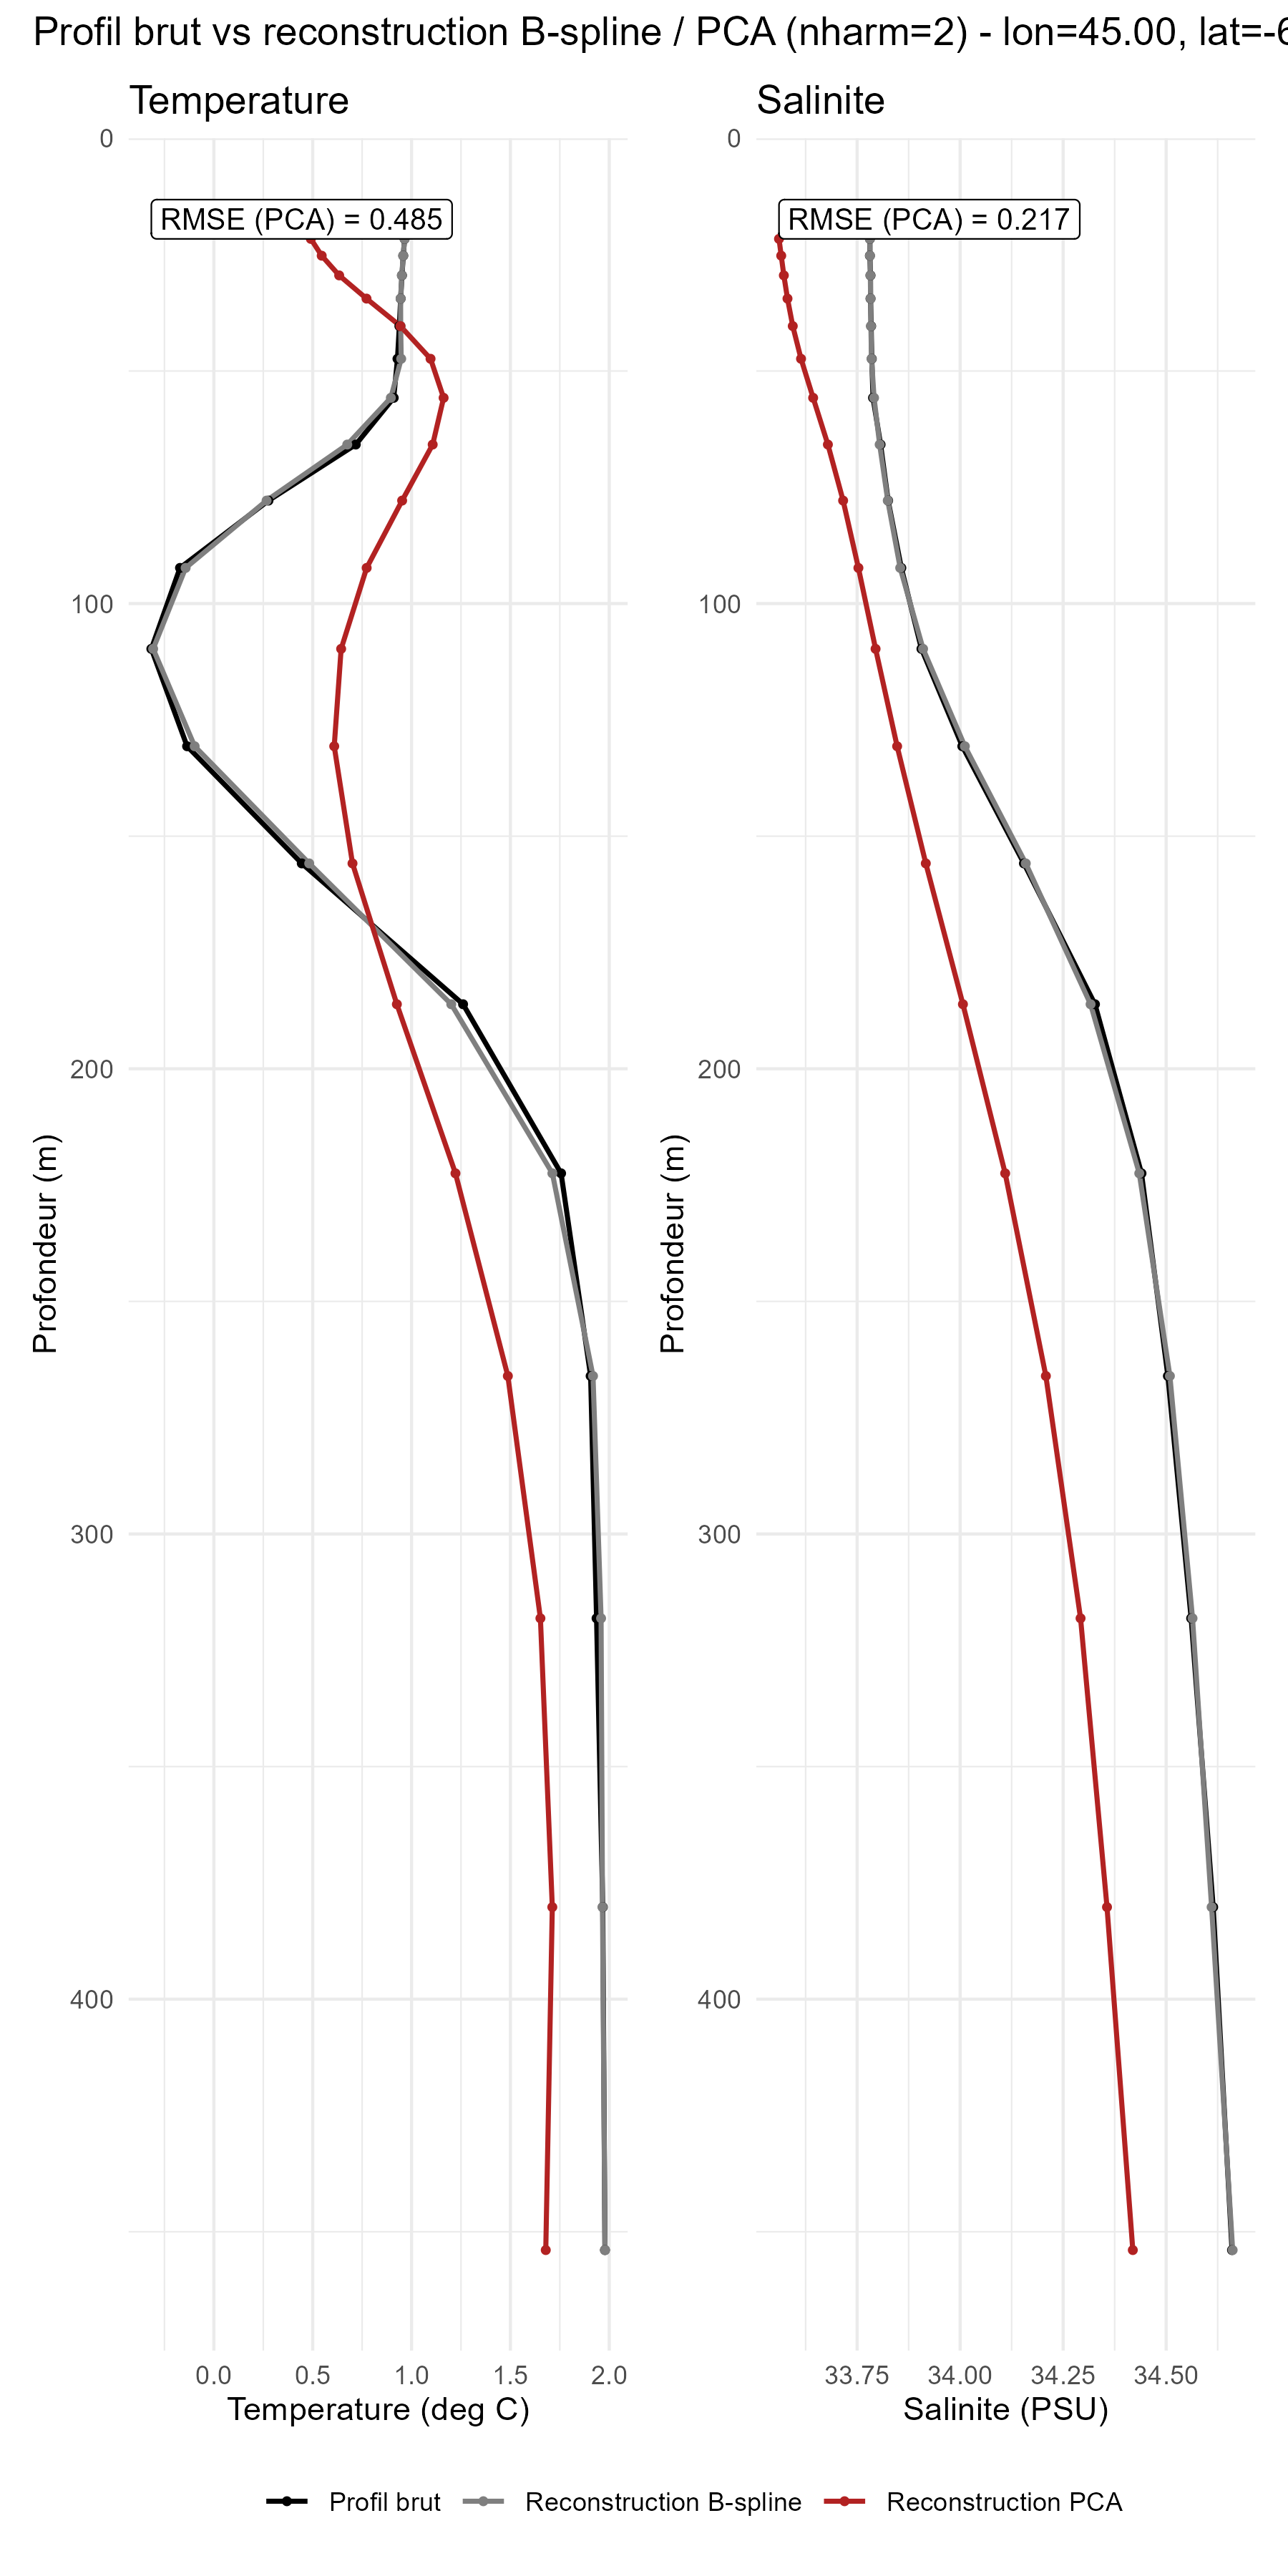
\includegraphics[width=\textwidth]{images/05_annexes/03_methode/profil_pca_temp_sal_lon45.00_lat-60.00_nharm2.00}
						\caption{$k=2$}
						\label{fig:profil_pca_k2}
					\end{subfigure}
					\hfill
					\begin{subfigure}{0.3\textwidth}
						\centering
						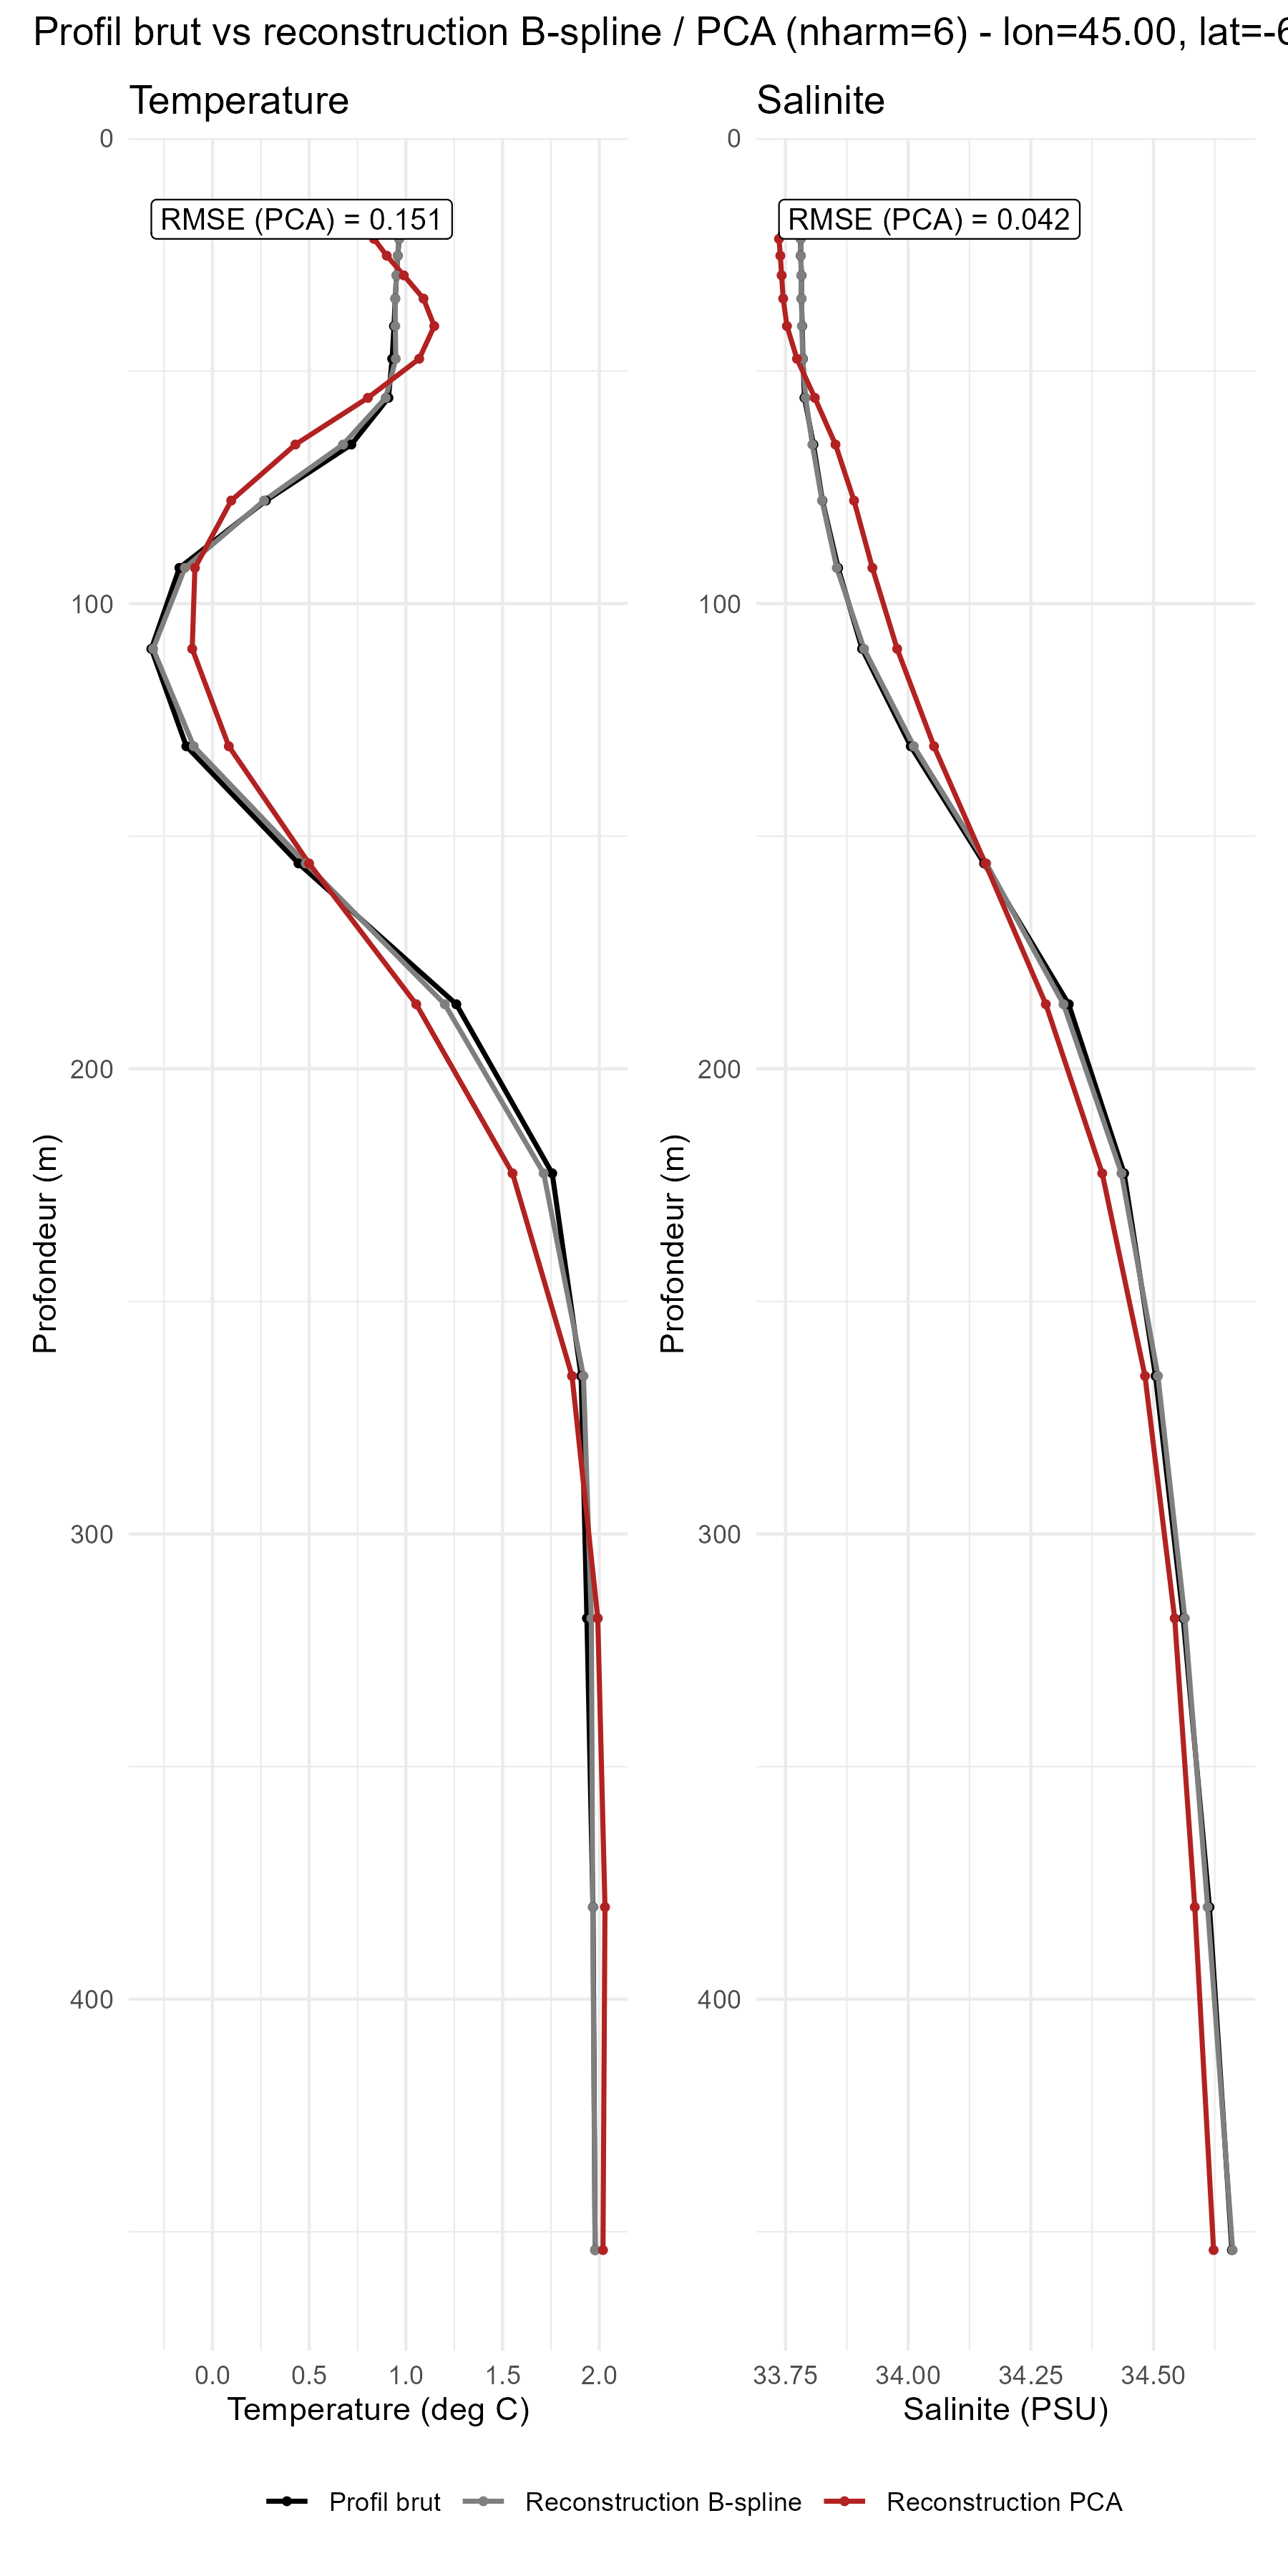
\includegraphics[width=\textwidth]{images/05_annexes/03_methode/profil_pca_temp_sal_lon45.00_lat-60.00_nharm6.00}
						\caption{$k=6$}
						\label{fig:profil_pca_k6}
					\end{subfigure}
					\hfill
					\begin{subfigure}{0.3\textwidth}
						\centering
						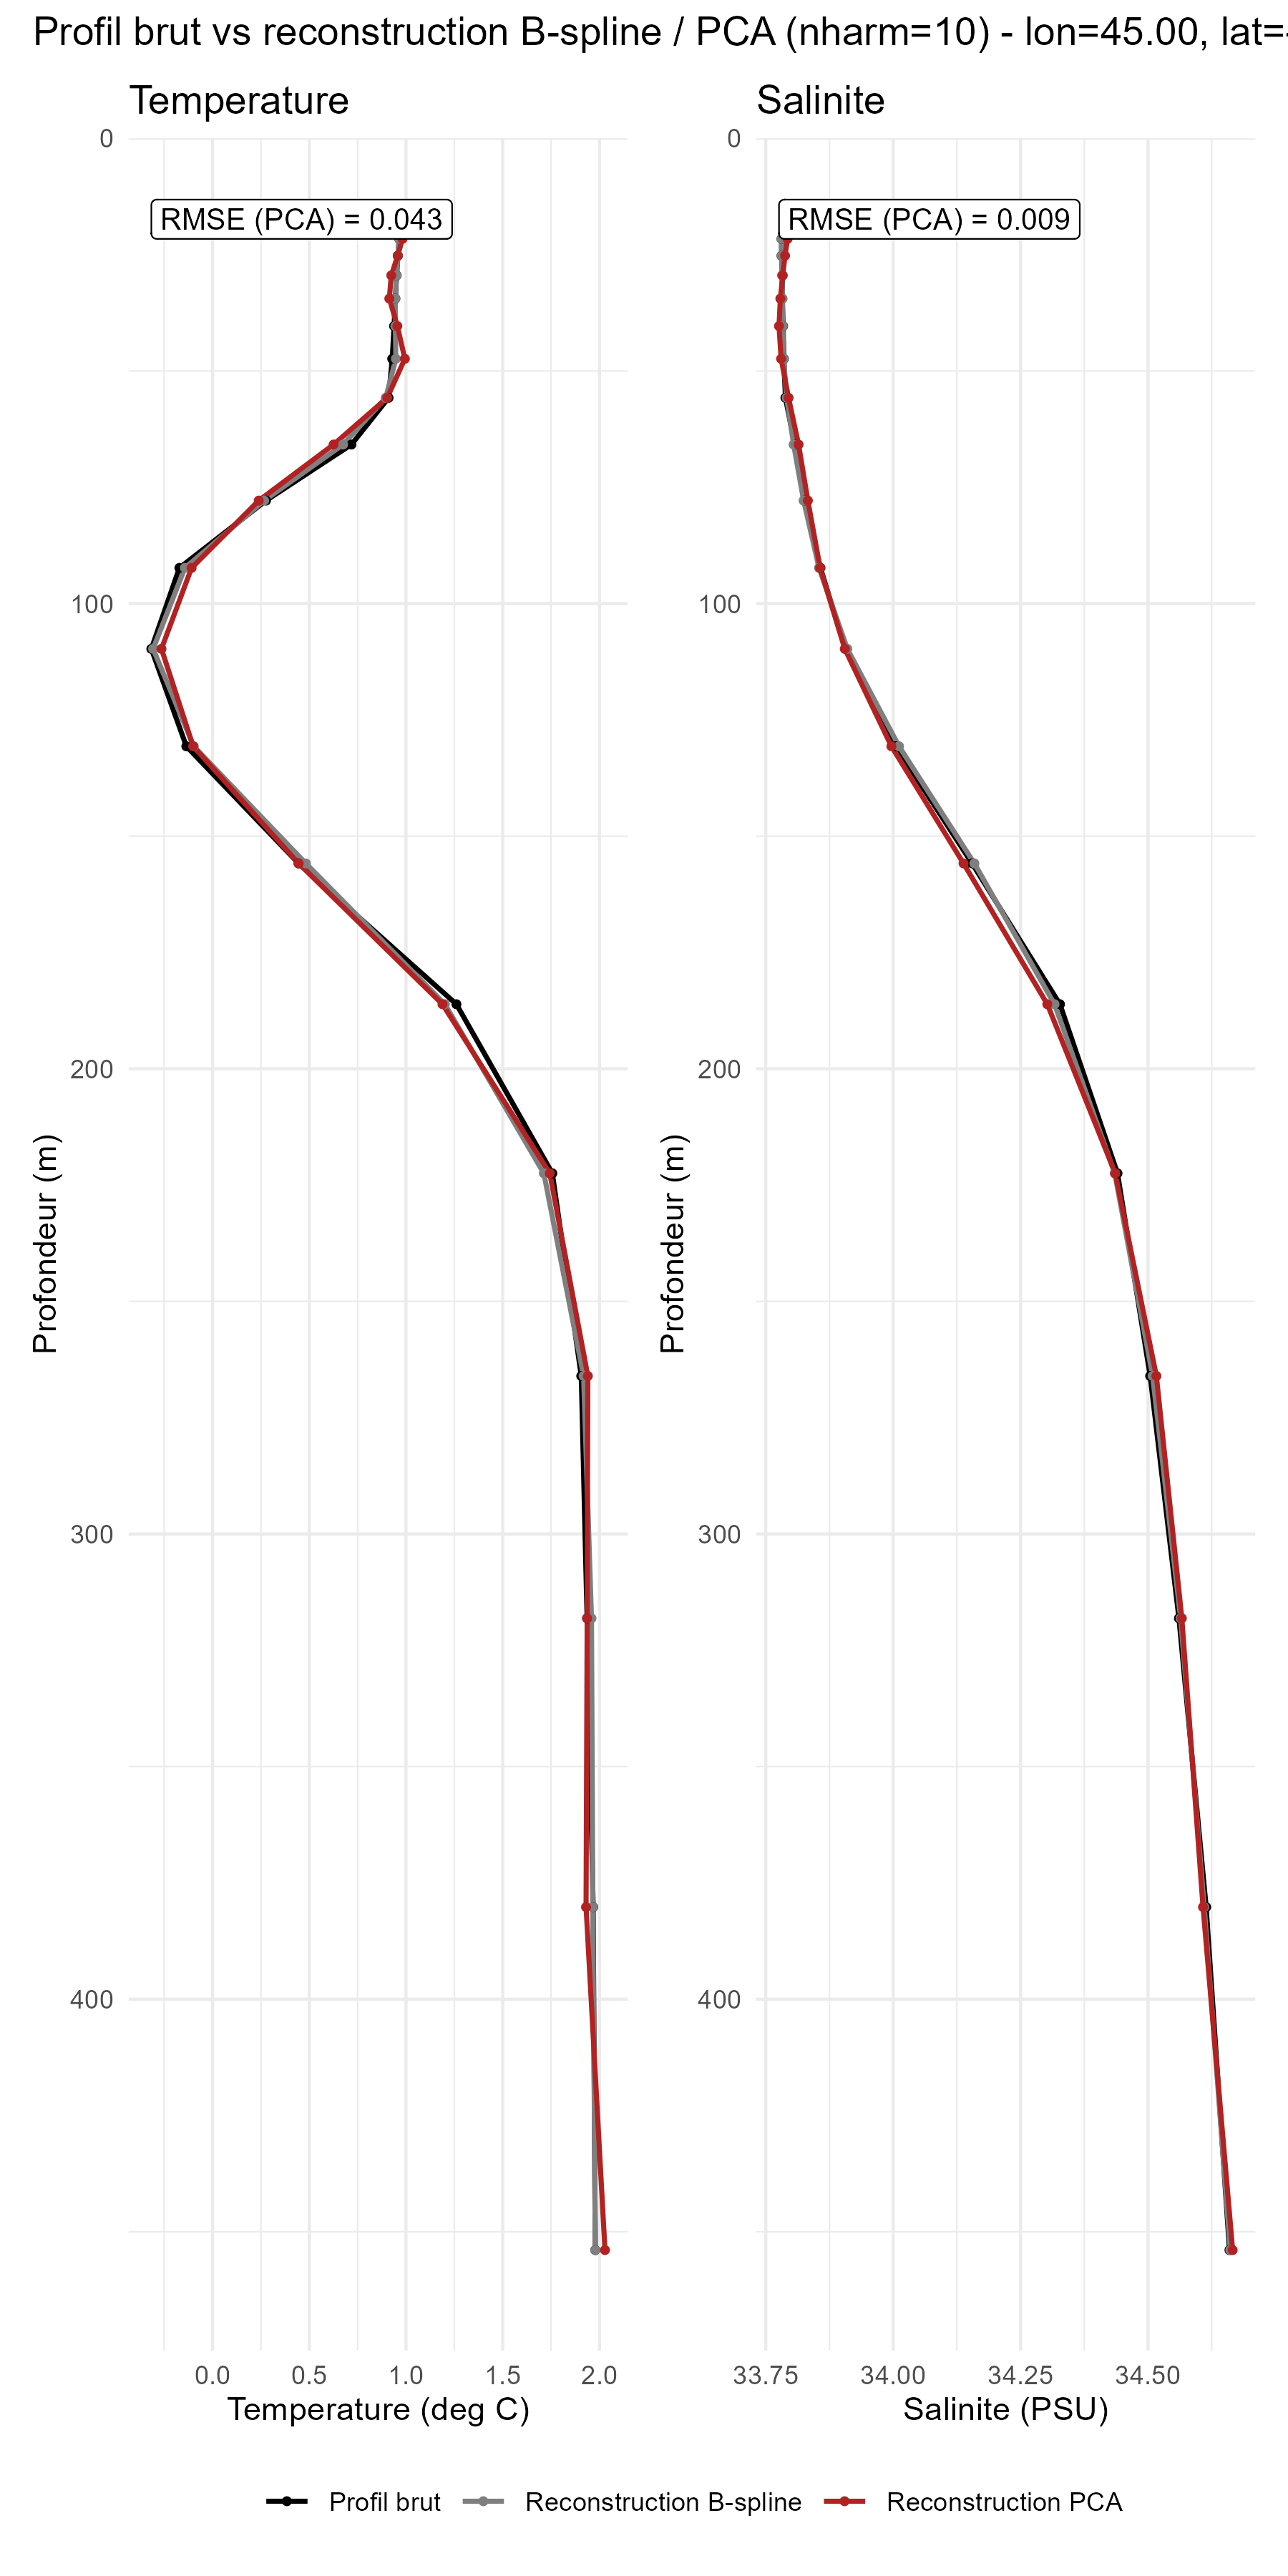
\includegraphics[width=\textwidth]{images/05_annexes/03_methode/profil_pca_temp_sal_lon45.00_lat-60.00_nharm10.00}
						\caption{$k=10$}
						\label{fig:profil_pca_k10}
					\end{subfigure}
					
					\caption{Effet du nombre de composantes principales $k$ sur la qualité de reconstruction des profils de température et salinité par sélection de $k$ PC puis projection sur des bases de B-splines. Un nombre de PC permettant d'obtenir une variance expliquée $>0.99$\% ne permet pas nécessairement une reconstruction correcte des profils.}
					\label{fig:profilpcatempsalcompare}
				\end{figure}
		
		
		\subsection{Gaussian Model Mixture Clustering}
		Afin de regrouper les profils de température et salinité similaires et identifier des Domaines Océanographiques Fonctionnels, on effectue un GMM clustering sur la matrice des coefficients réduite $c$ obtenue à l'étape précédente. Le fonctionnement de la méthode ne sera pas développée ici, se référer a \cite{bishop2006pattern} pour une explication. Le GMM clustering a été implémenté avec le package mclust \cite{scrucca2016mclust}, \cite{fraley2002mclust} disponible sous R. Le modèle le plus flexible (model="VVV") a été utilisé, permettant un ajustement des ellipsoïde non contraint en volume, orientation et forme, celà au prix d'une augmentation du nombre d'hyperparamètres. Avec les précédents travaux réalisés par Fonvieille N. et Molinet M. \cite{fonvieille2024}, \cite{molinetLinkingOceanographic}, la recherche d'une nombre de cluster a été restreinte entre 4 et 6 clusters, réduisant ainsi le coût computationnel. Les clusters ont été définis lorsque la probabilité d'appartenance à un cluster était suppérieur au seuil fixé à 0.75. Des classes de transitions ont été créées en fonction des deux clusters ayant une probabilité d'appartenance maximale. 
		
		
		
	\section{Clustering des données pigmentaires}
		\label{annexe : cluster_pig}
		\begin{figure}[H]
			\centering
			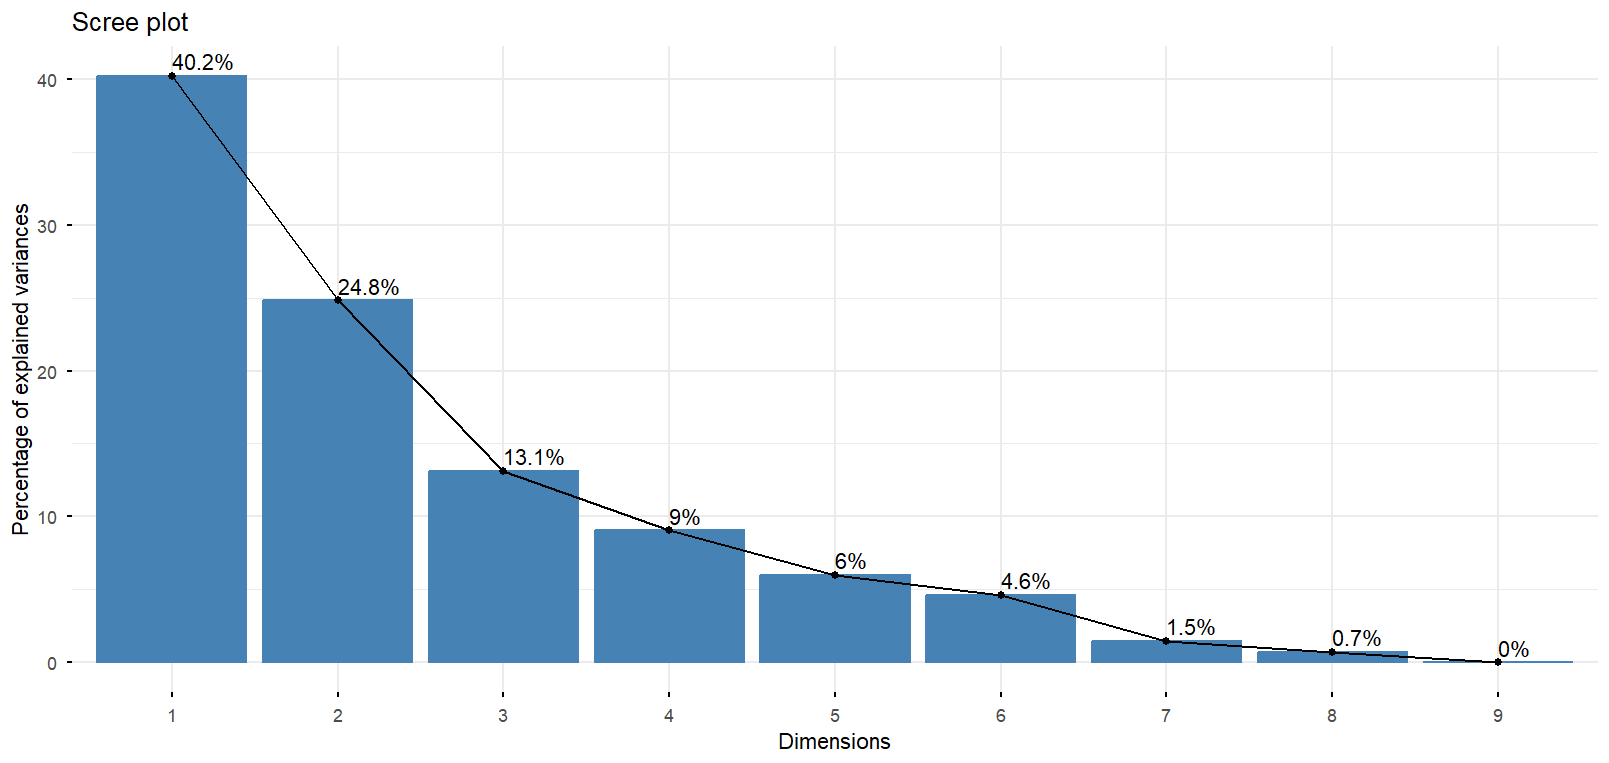
\includegraphics[width=0.8\textwidth]{images/05_annexes/04_resultats/comu_phyto_cluster_pigs/explained_var}
			\caption{Histogramme de la variance expliquée par composante principale (triées par ordre décroissantes)}
			\label{fig:explainedvarpig}
		\end{figure}
		\begin{figure}[H]
			\centering
			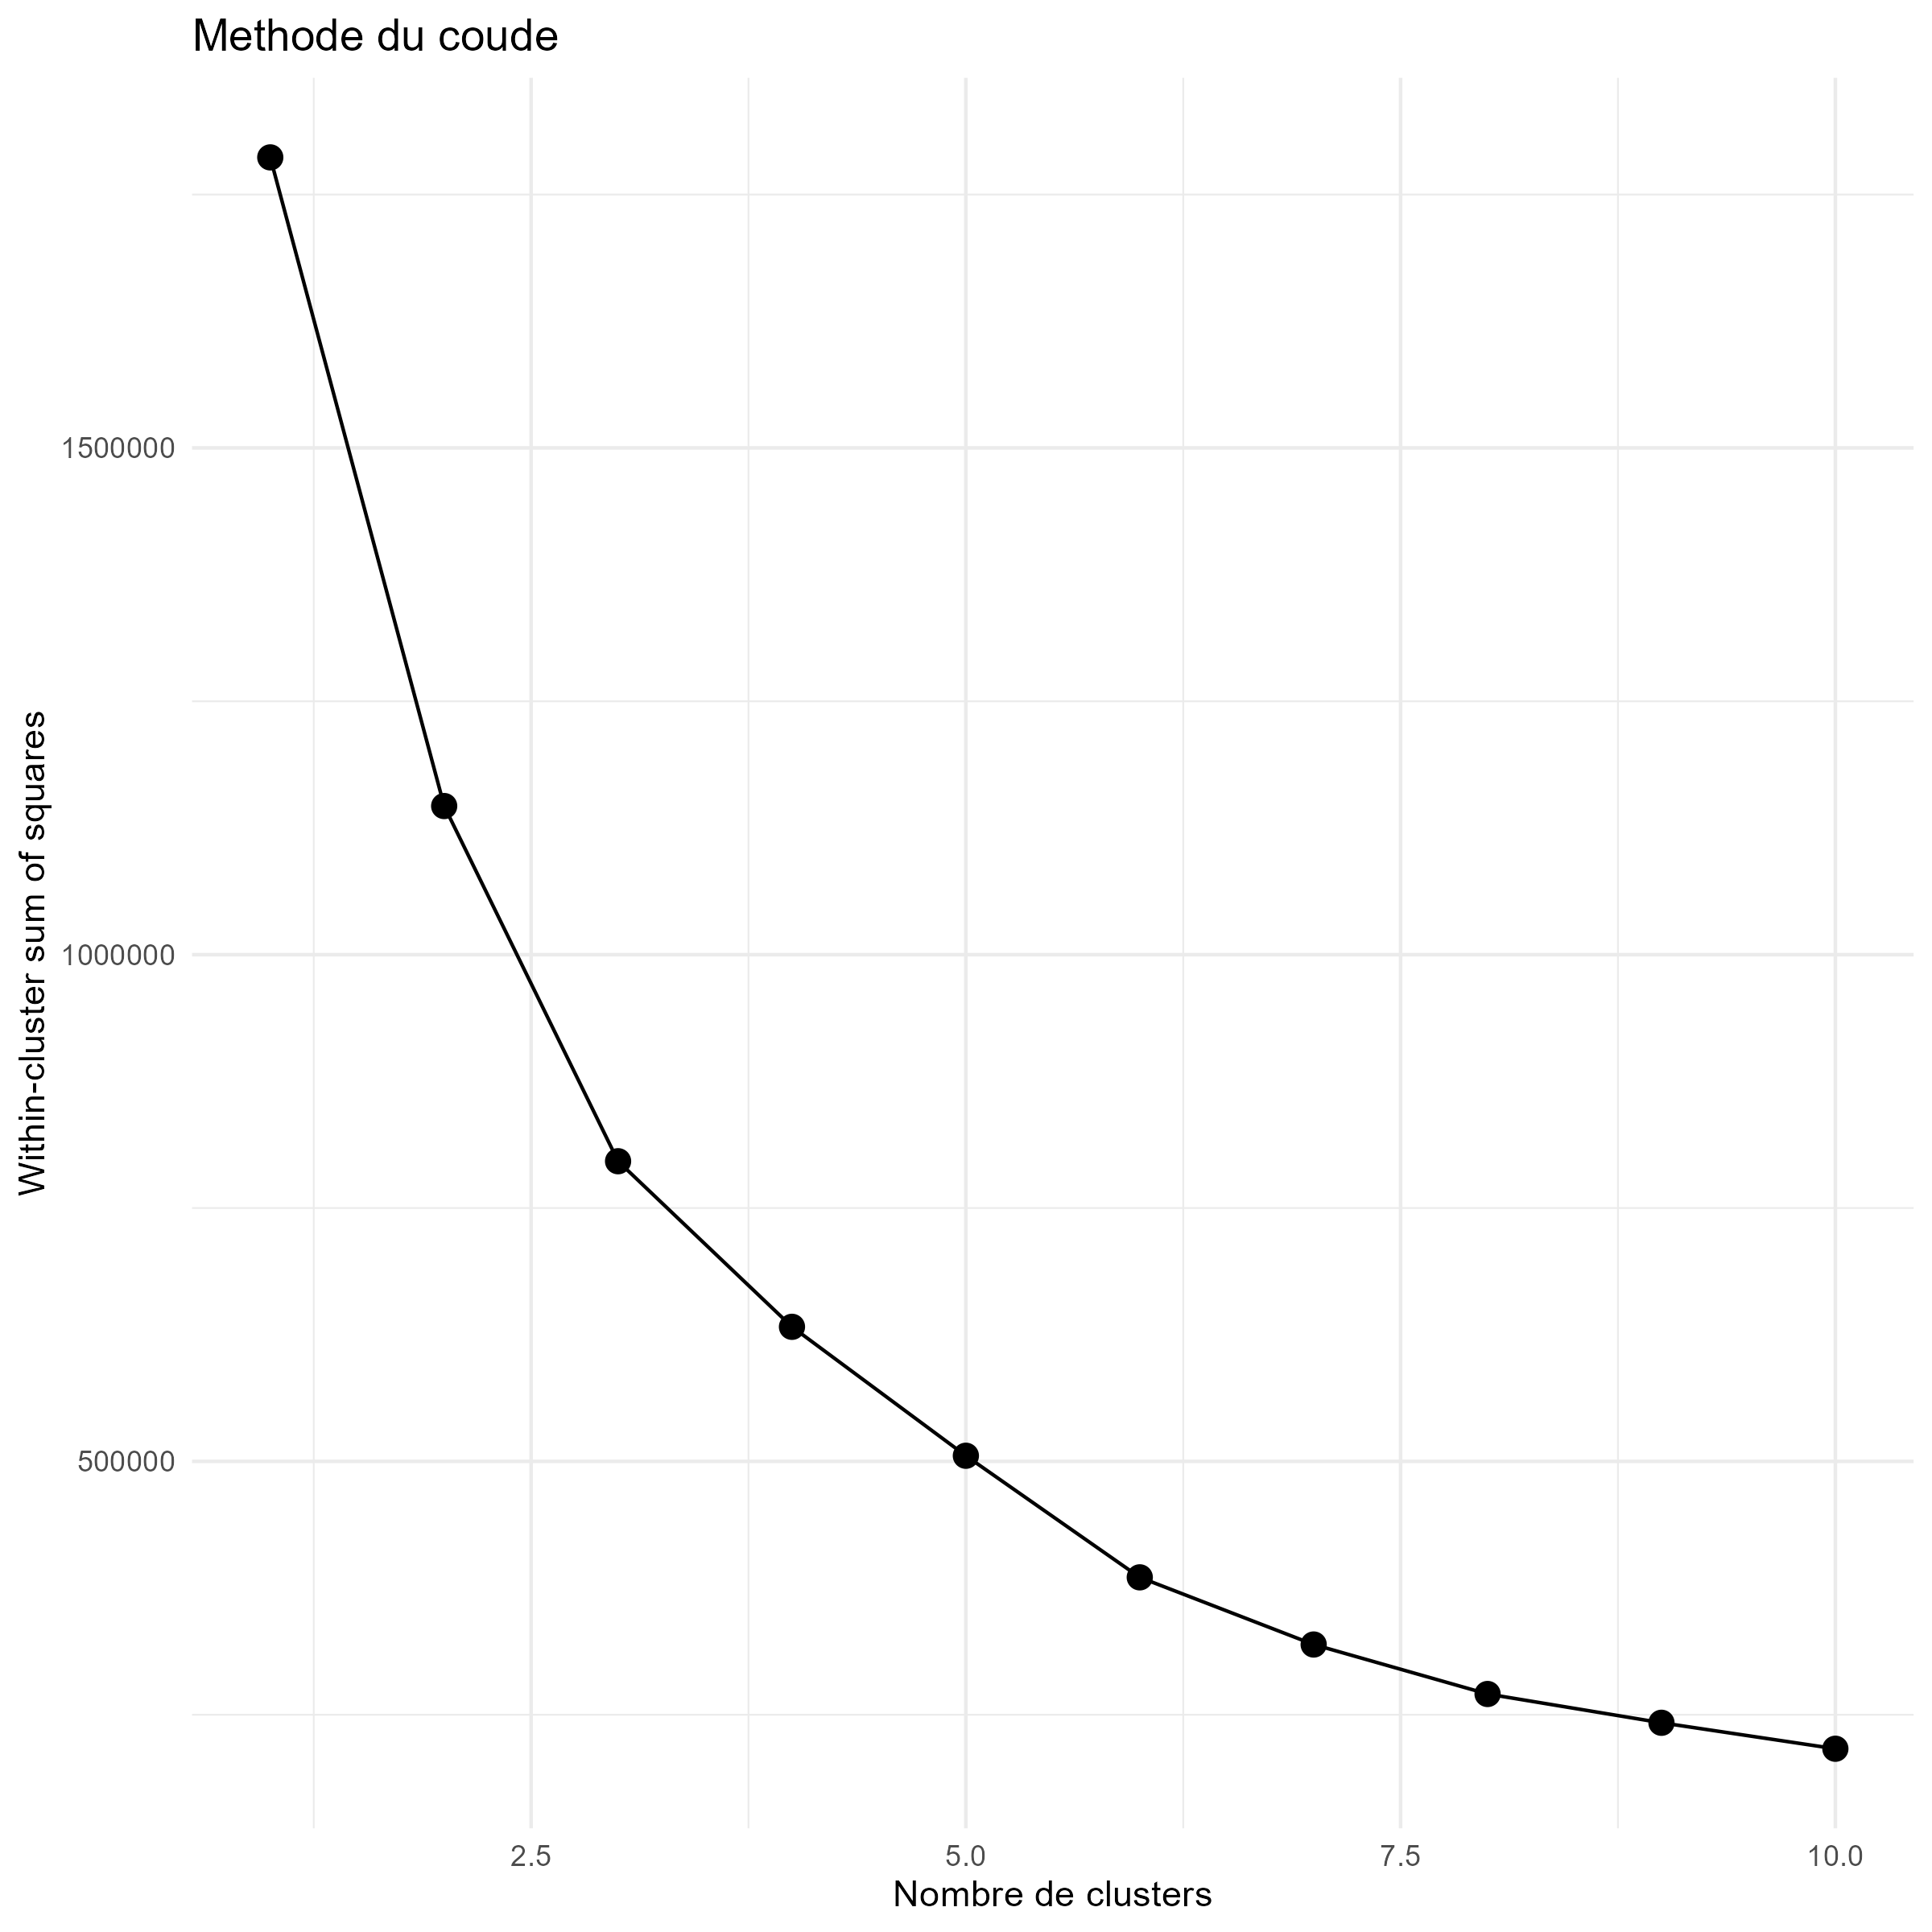
\includegraphics[width=0.6\textwidth]{images/05_annexes/04_resultats/comu_phyto_cluster_pigs/elbow_method_kmeans}
			\caption{Méthode du coude (Elbow method) : inertie intra-classe (somme des carrés intra-cluster) en fonction du nombre de cluster.}
			\label{fig:elbowmethodkmeans}
		\end{figure}
			
	\section{Choix du modèle de validation croisée}
		\label{annexe:choix_valid_croisee_autocorr}
		\begin{figure}
			\centering
			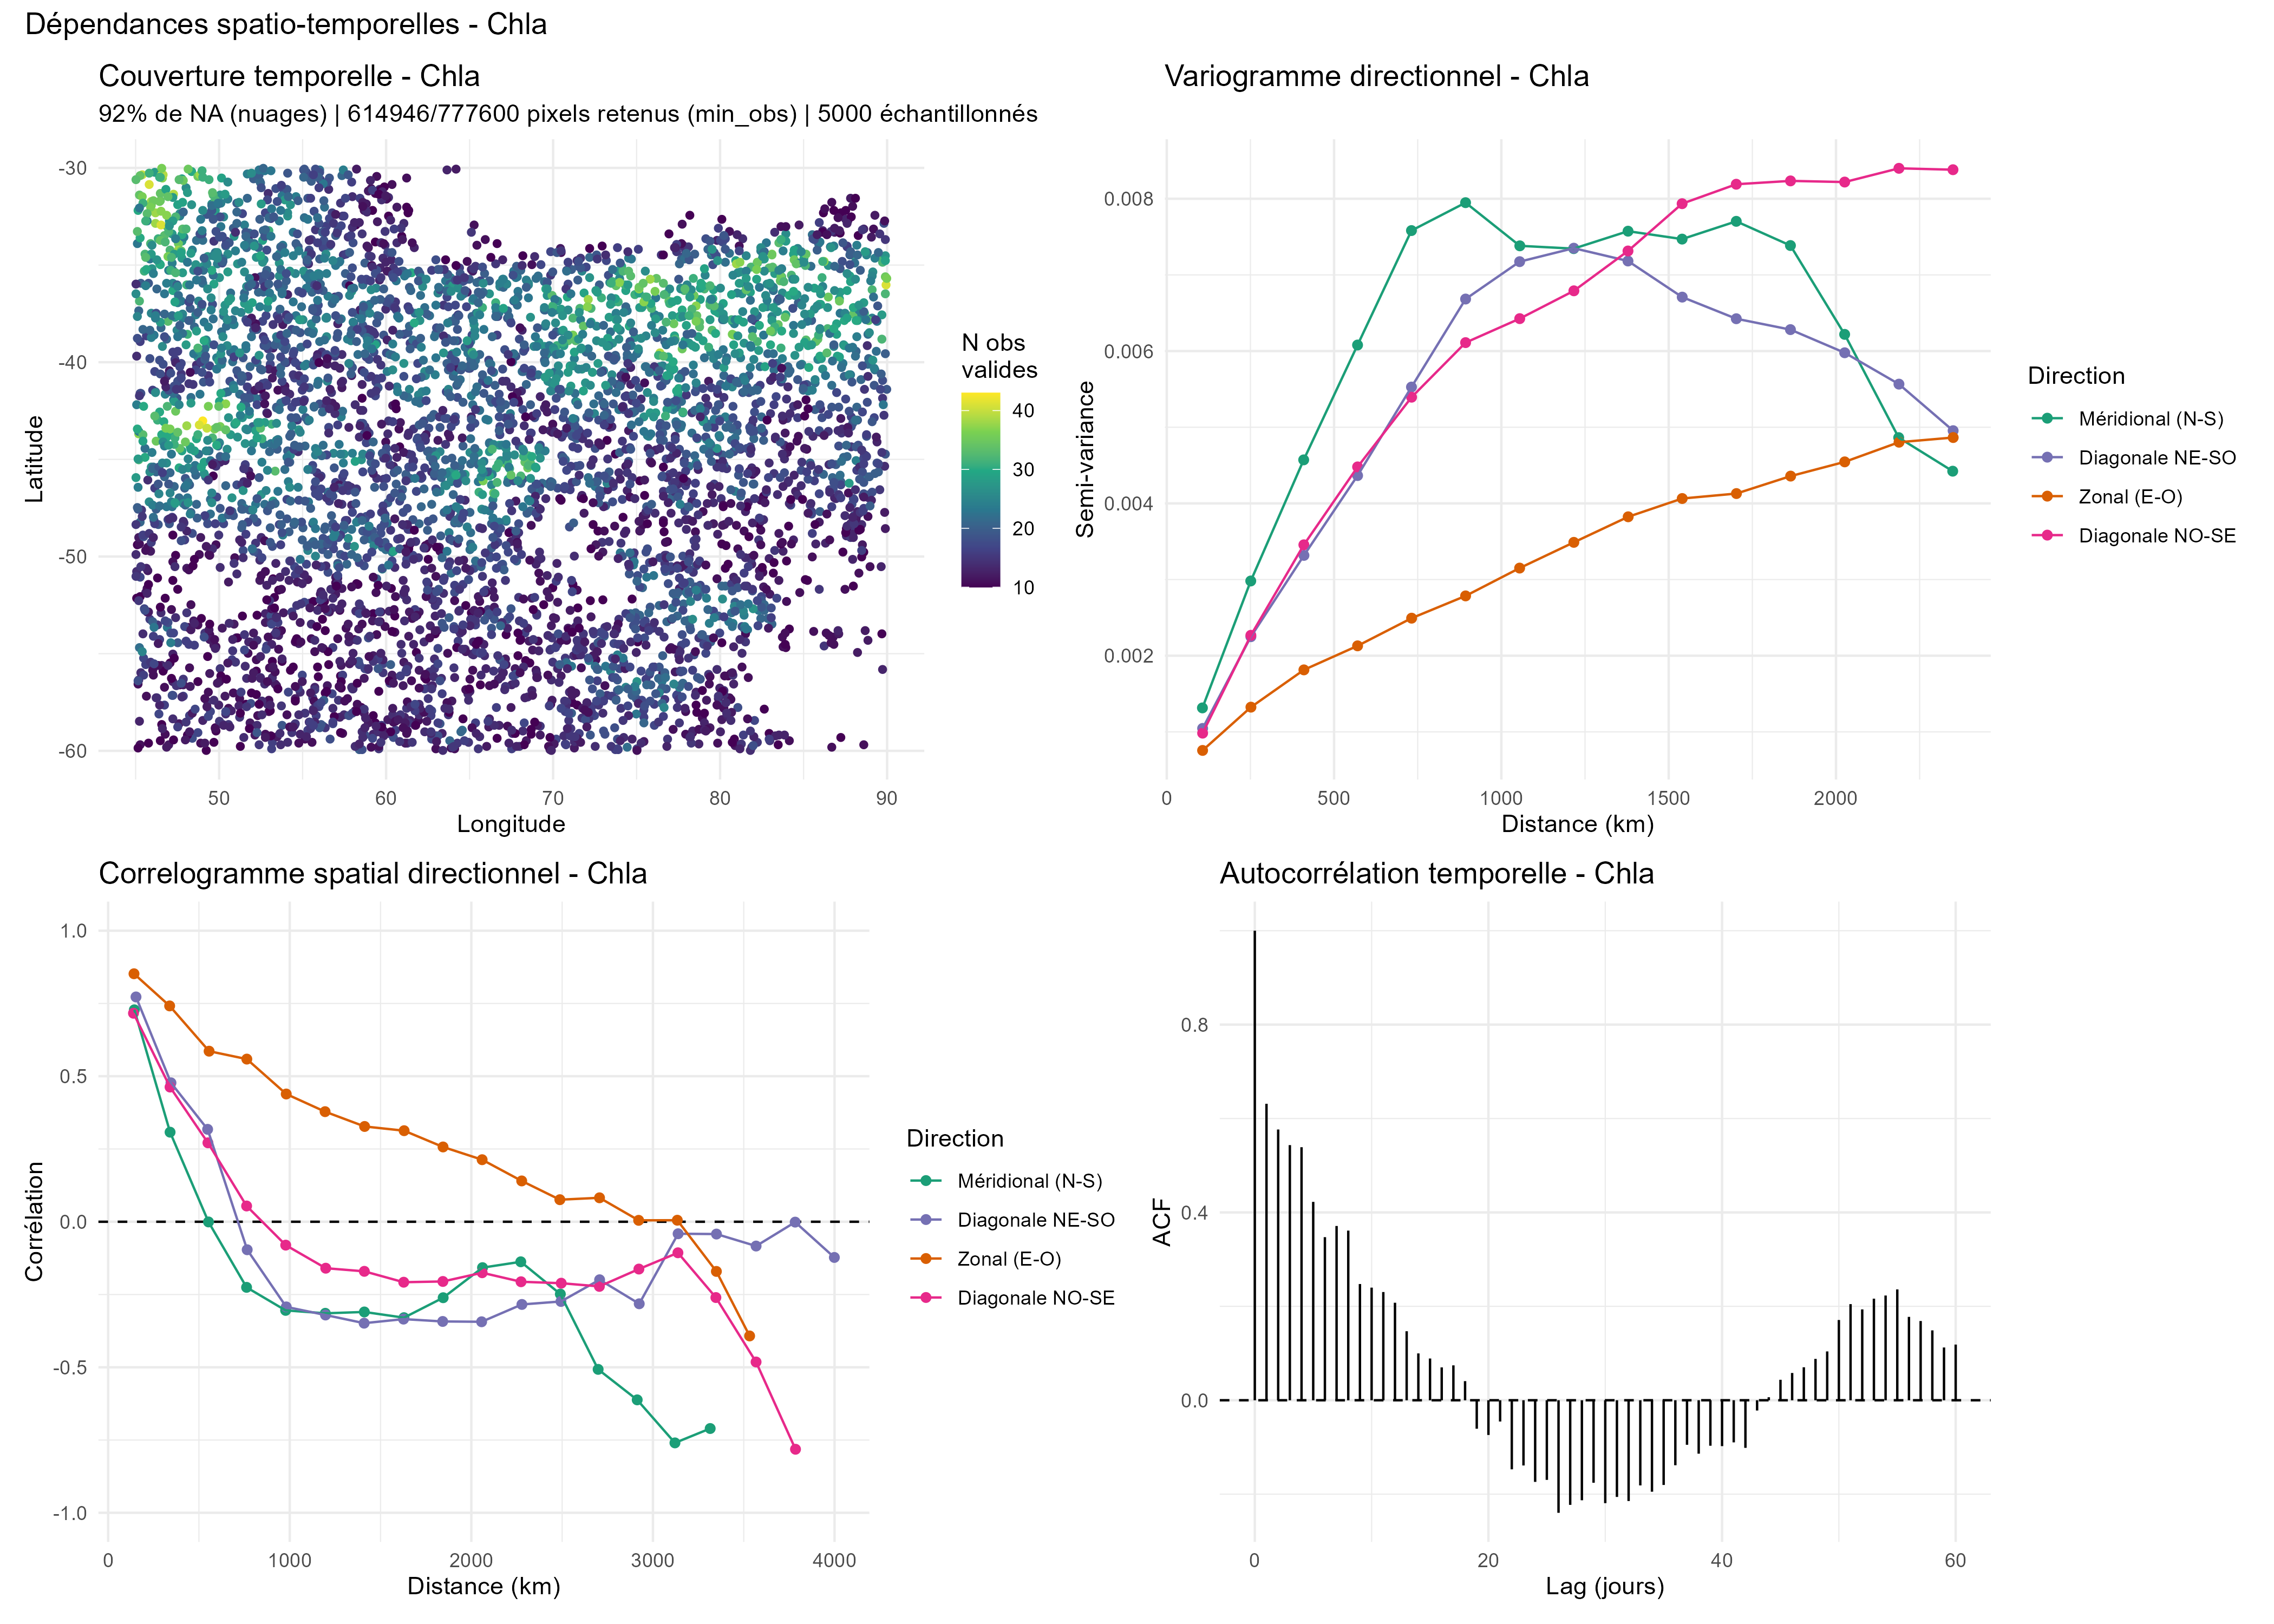
\includegraphics[width=\linewidth]{images/05_annexes/02_materiel/autocorrelation_spatio_temp/diag_autocorrelation_spatio_temp_chla}
			\caption{Diagnostique d'autocorrelation spatio-temporelle de la chlorophylle-a sur l'ensemble de la ROI et des années d'étude (2018, 2021, 2022, 2023, janvier-mars)}
			\label{fig:diagautocorrelationspatiotempchla}
		\end{figure}
		\begin{figure}
			\centering
			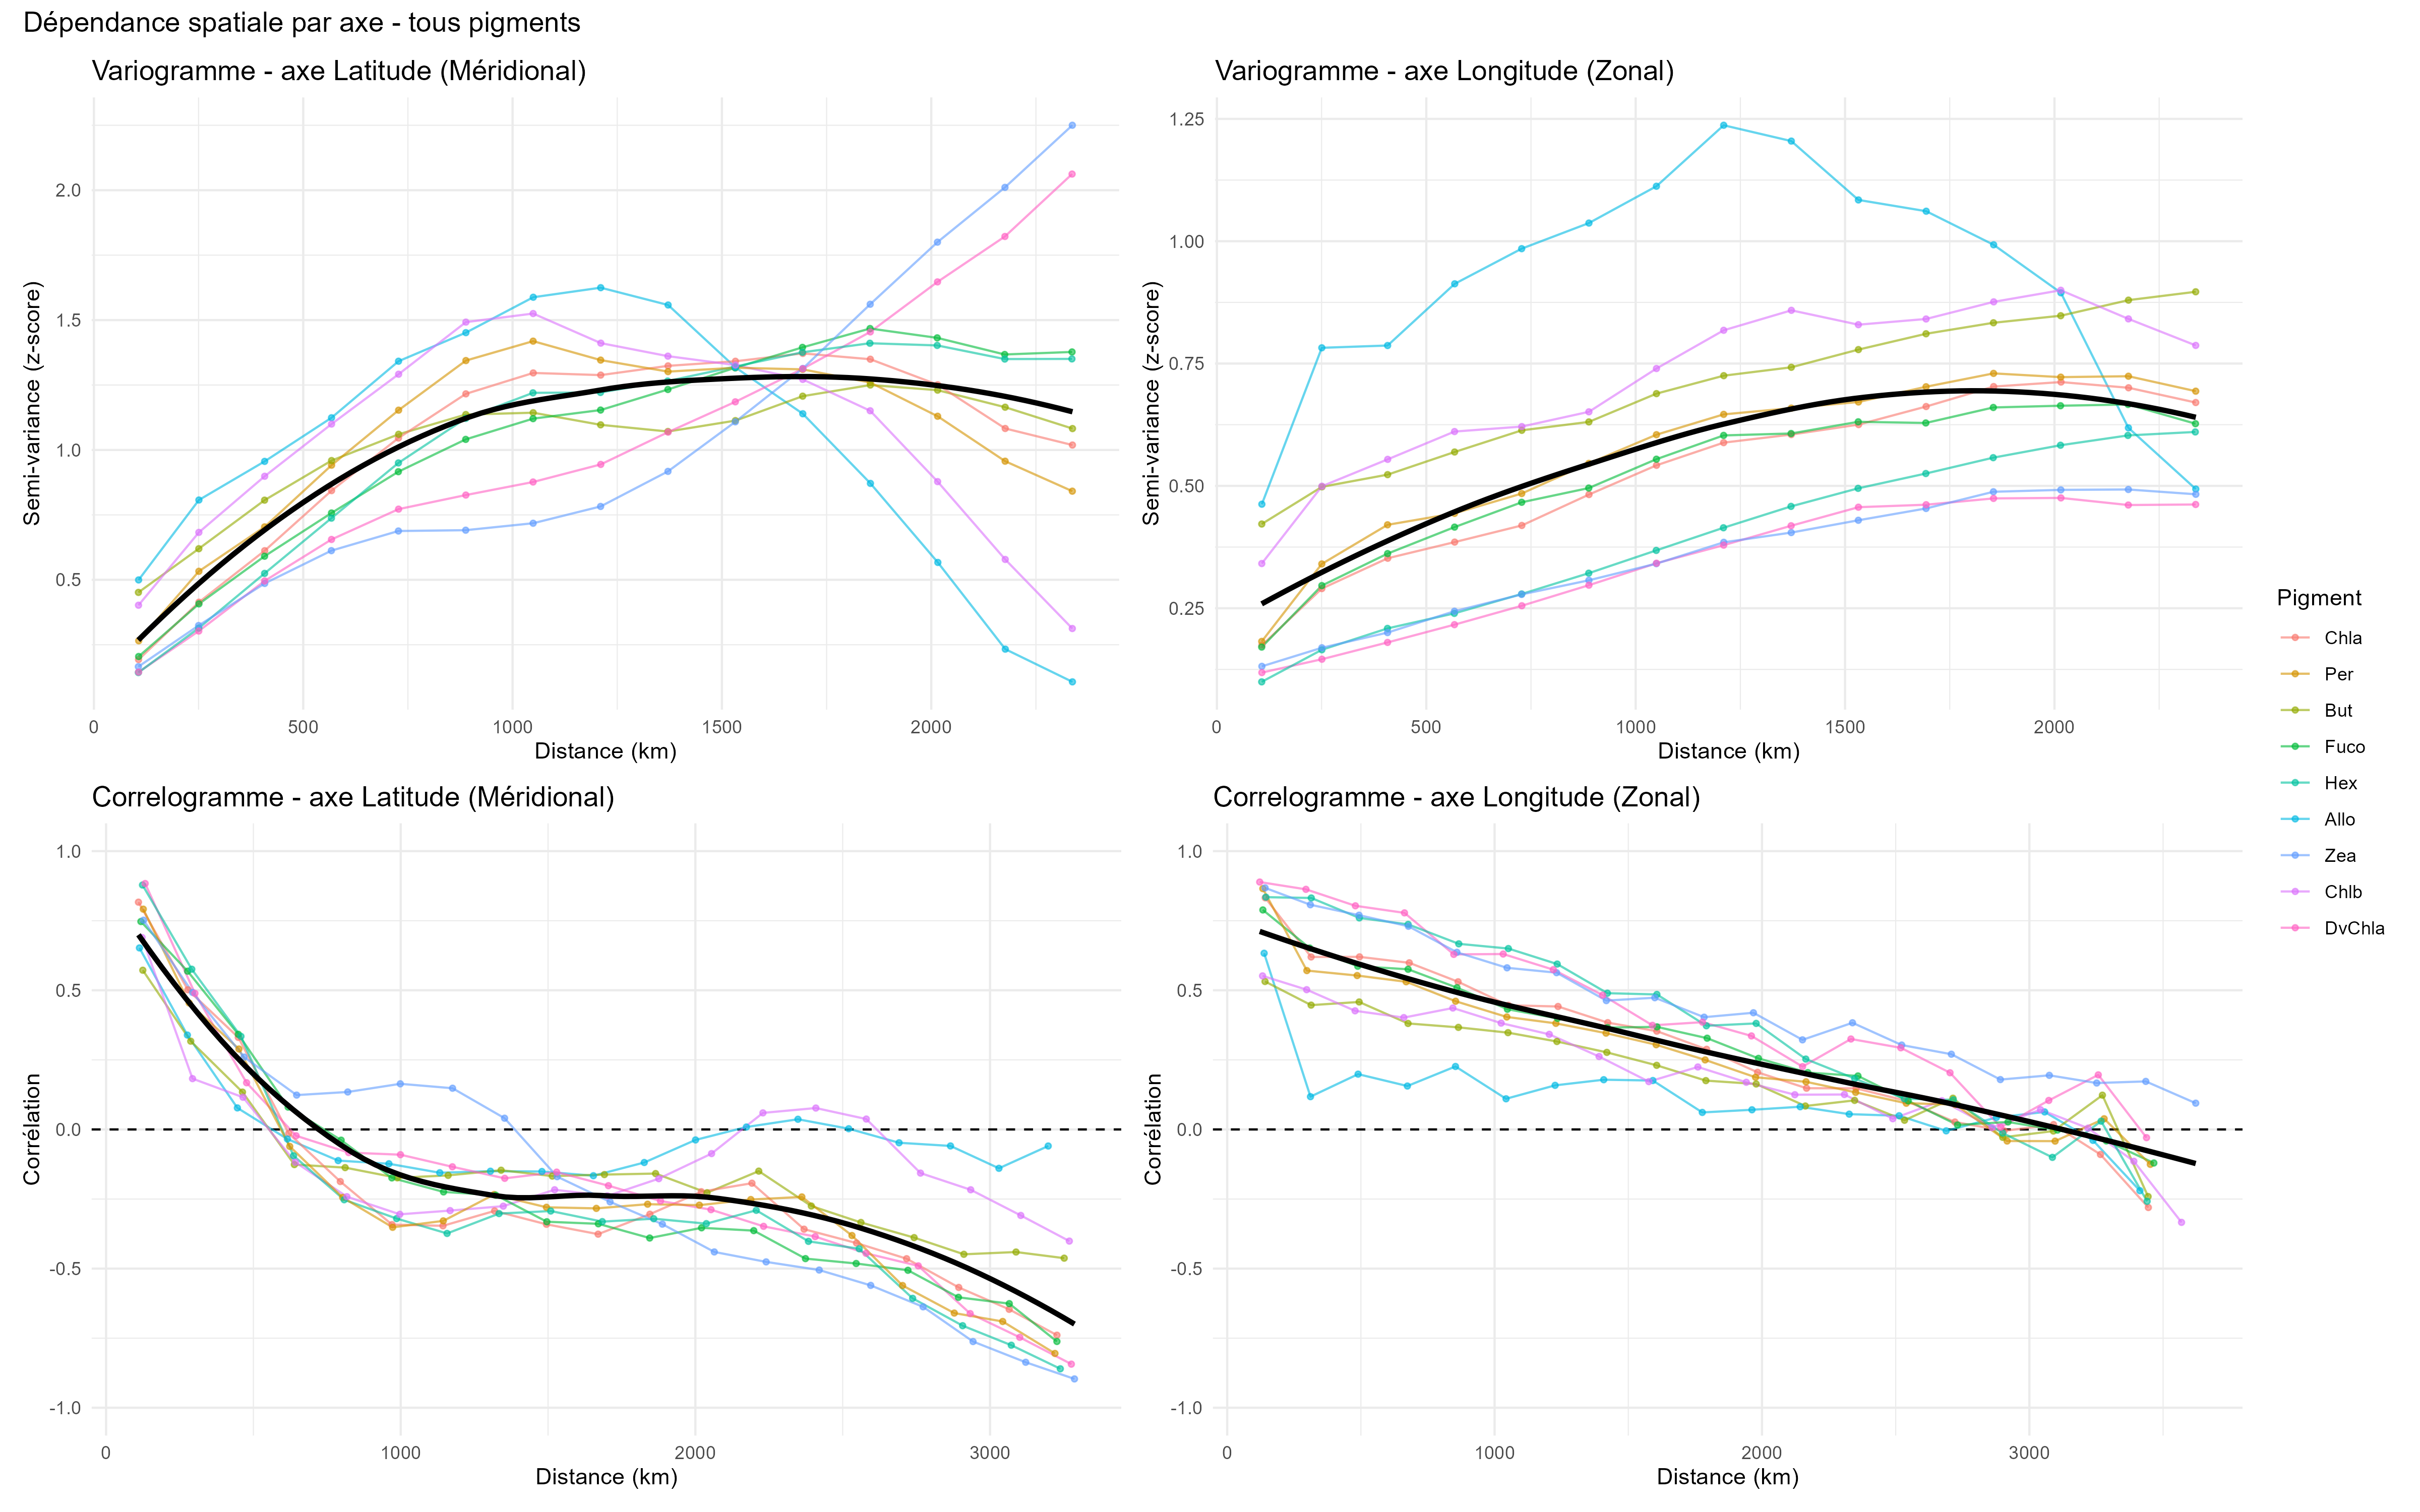
\includegraphics[width=\linewidth]{images/05_annexes/02_materiel/autocorrelation_spatio_temp/diag_autocorrelation_lat_lon_tous_pigments}
			\caption{Diagnostique d'autocorrelation spatio-temporelle de l'ensemble des pigments photosynthétiques, sur toute la ROI et sur toutes les années d'étude (2018, 2021, 2022, 2023, janvier-mars)}
			\label{fig:diagautocorrelationlatlontouspigments}
		\end{figure}
		\begin{figure}
			\centering
			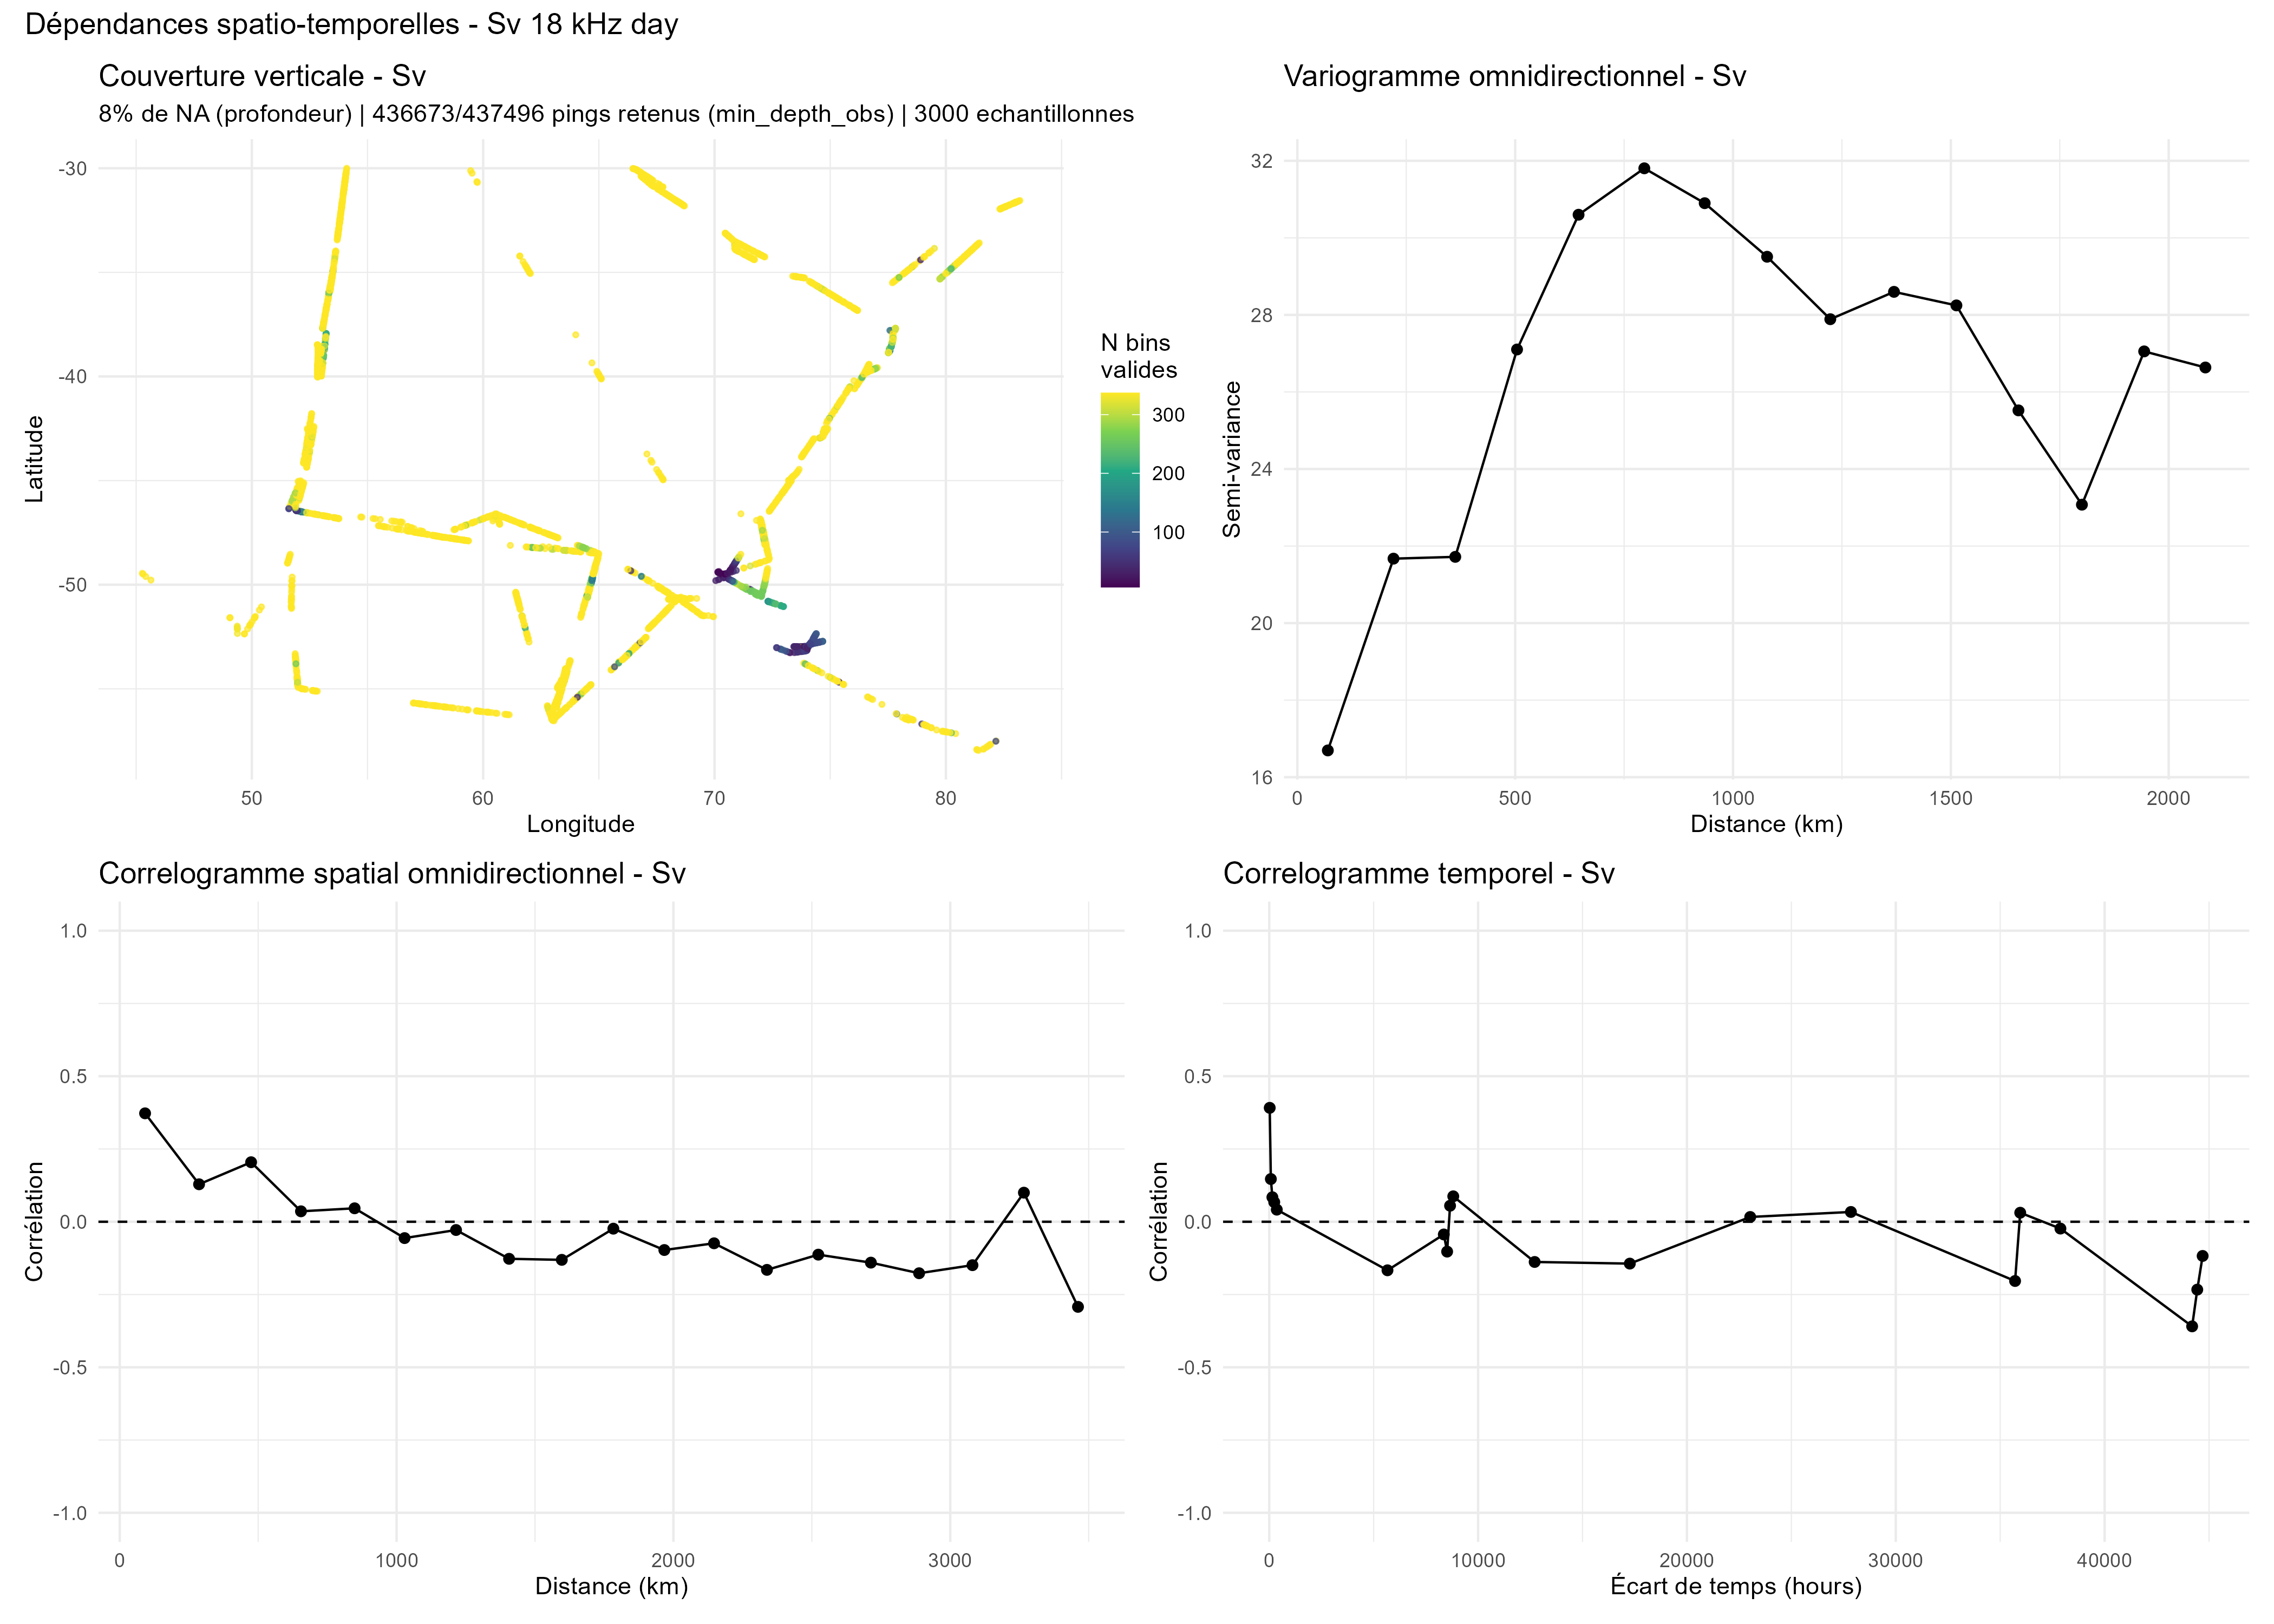
\includegraphics[width=0.8\linewidth]{images/05_annexes/02_materiel/autocorrelation_spatio_temp/diag_autocorrelation_spatio_temp_Sv_18kHz_day}
			\caption{Diagnostique d'autocorrelation spatio-temporelle du NASC (38kHz, jour) sur l'ensemble des transects (2018, 2021, 2022, 2023, janvier-mars)}
			\label{fig:diagautocorrelationspatiotempsv18khzday}
		\end{figure}
		\begin{figure}
			\centering
			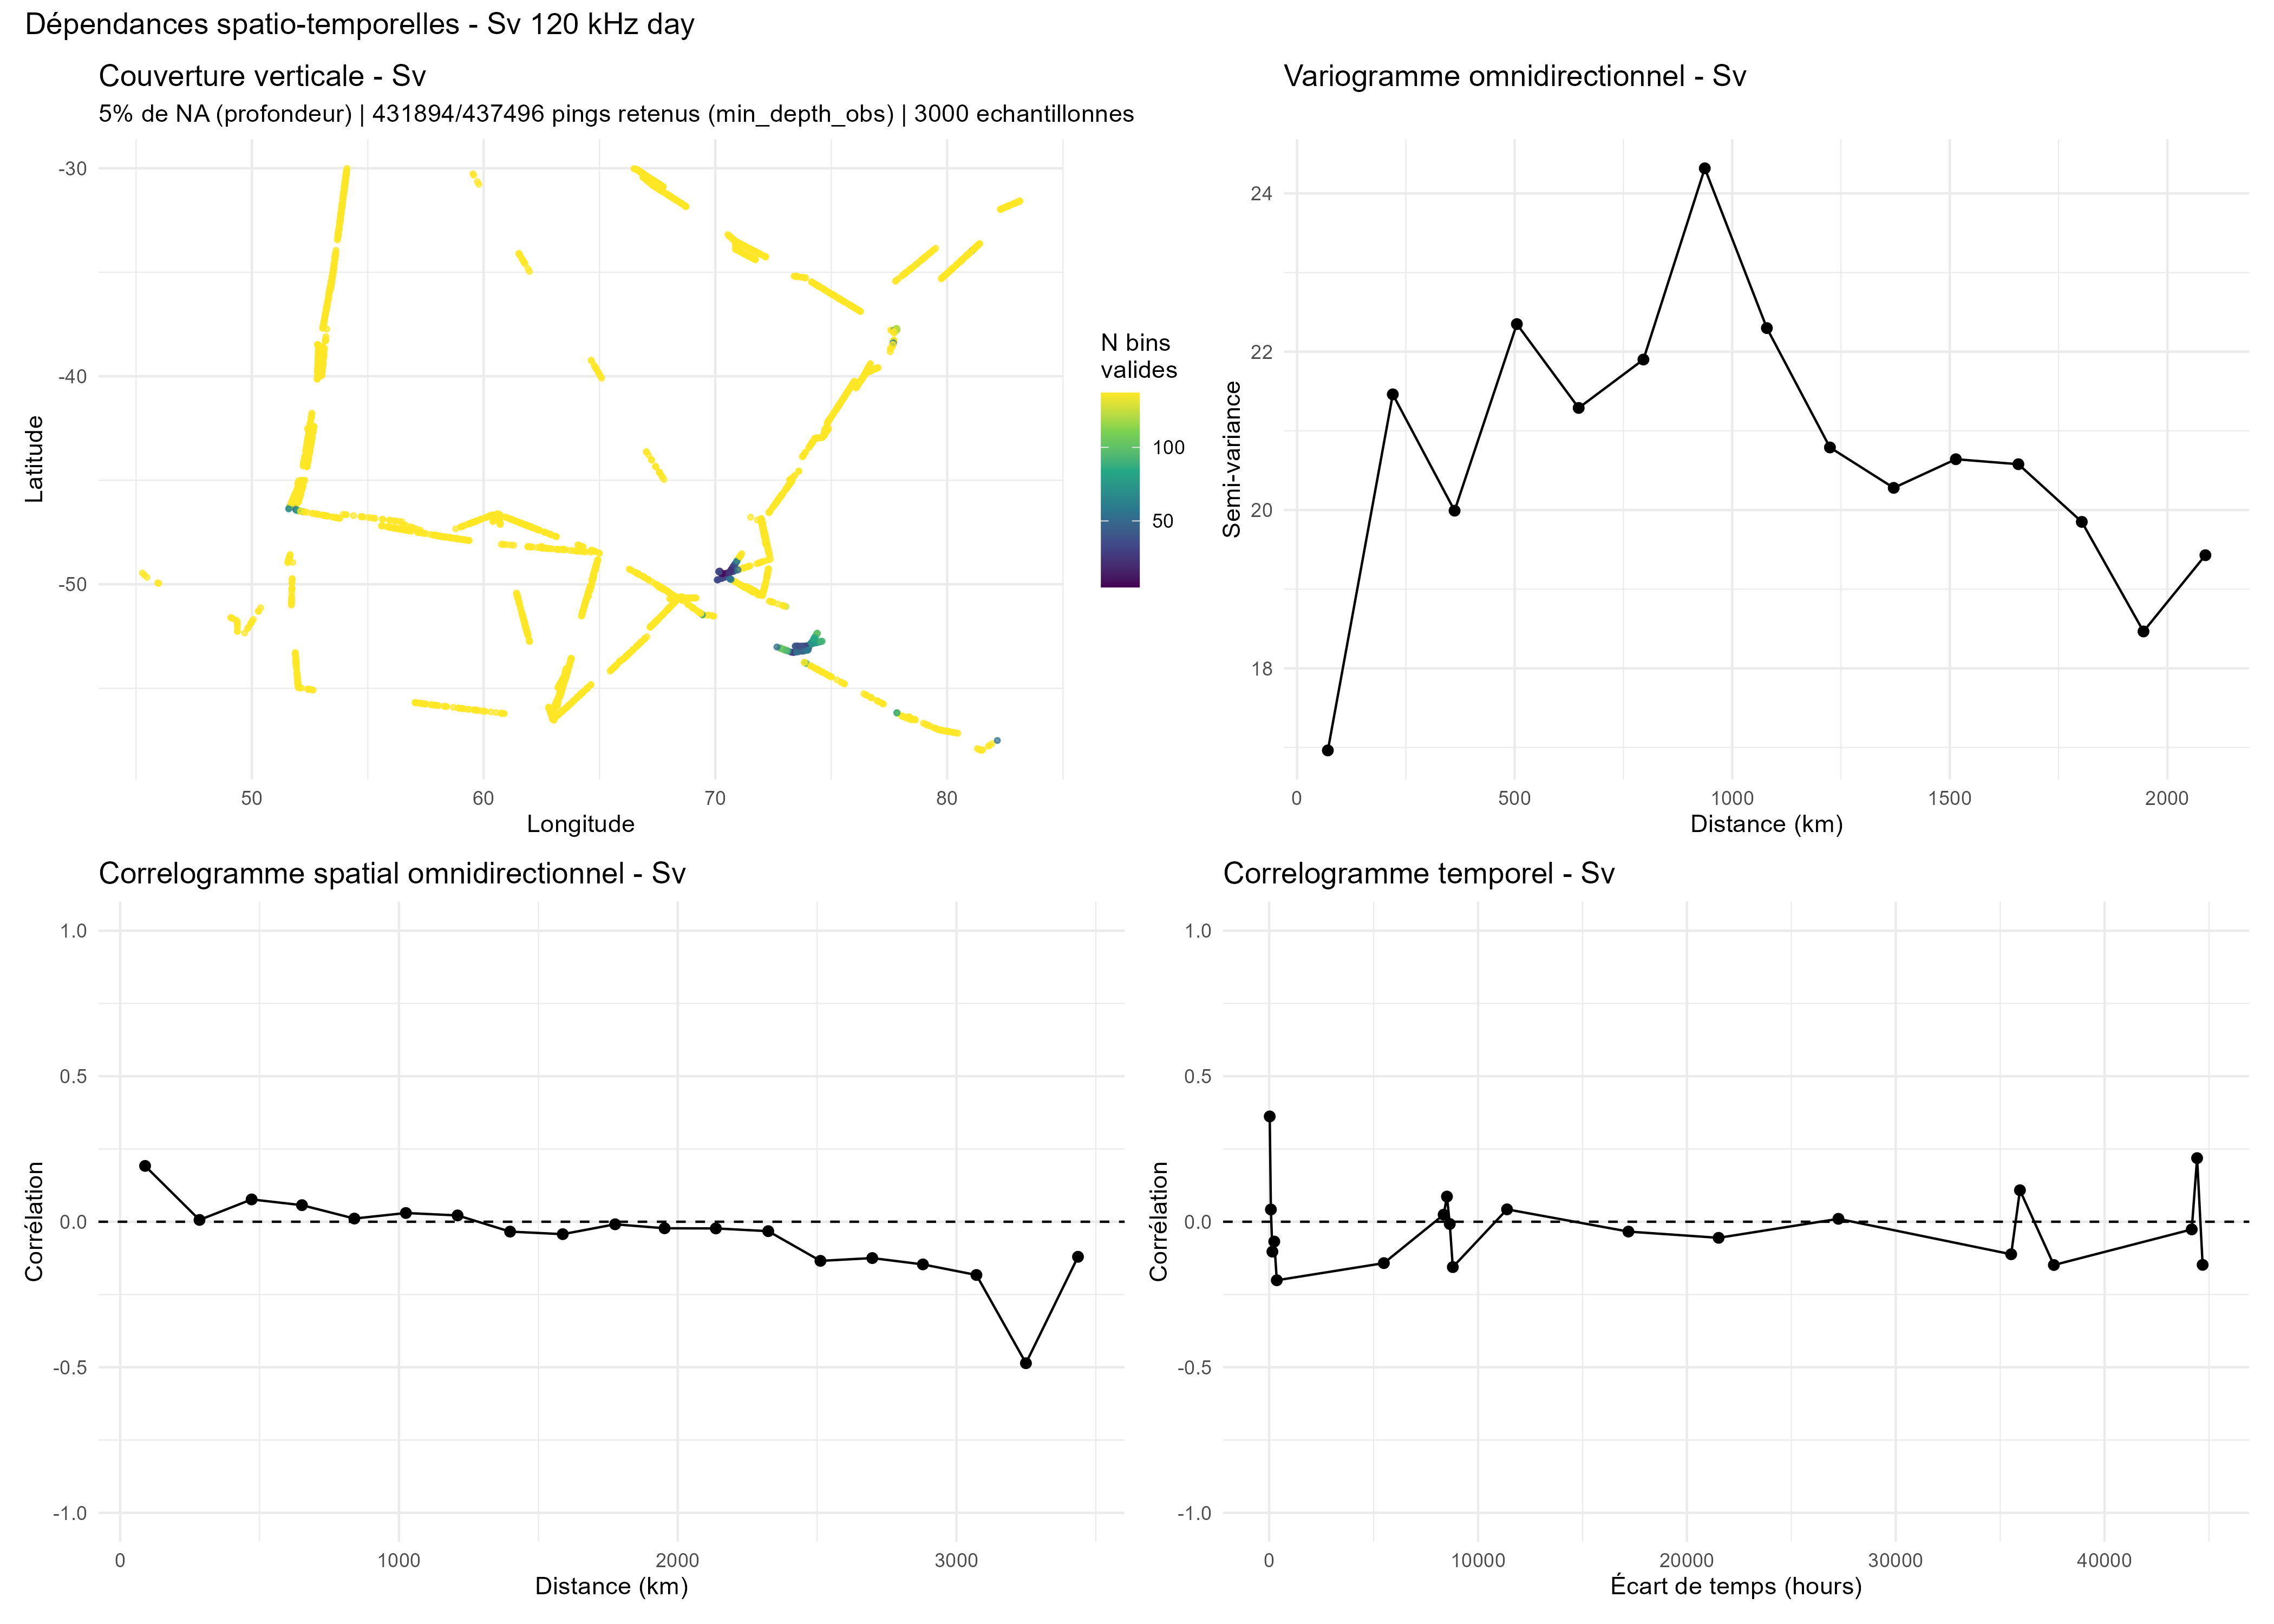
\includegraphics[width=0.8\linewidth]{images/05_annexes/02_materiel/autocorrelation_spatio_temp/diag_autocorrelation_spatio_temp_Sv_120kHz_day}
			\caption{Diagnostique d'autocorrelation spatio-temporelle du NASC (120kHz, jour) sur l'ensemble des transects (2018, 2021, 2022, 2023, janvier-mars)}
			\label{fig:diagautocorrelationspatiotempsv120khzday}
		\end{figure}
	
	\section{Résultats de tuning des modèles}
		\label{annexe:tuning_res}
		faire un tableau et mettre les graphiques de tuning générés
	
	
	% Résultats
	\section{Distribution des variables (NASC, FTLE et pigments)}
		\subsection{Nombre de données utilisées par année}
			\label{annexe:n_data_distribs}
			\begin{figure}[H]
				\centering
				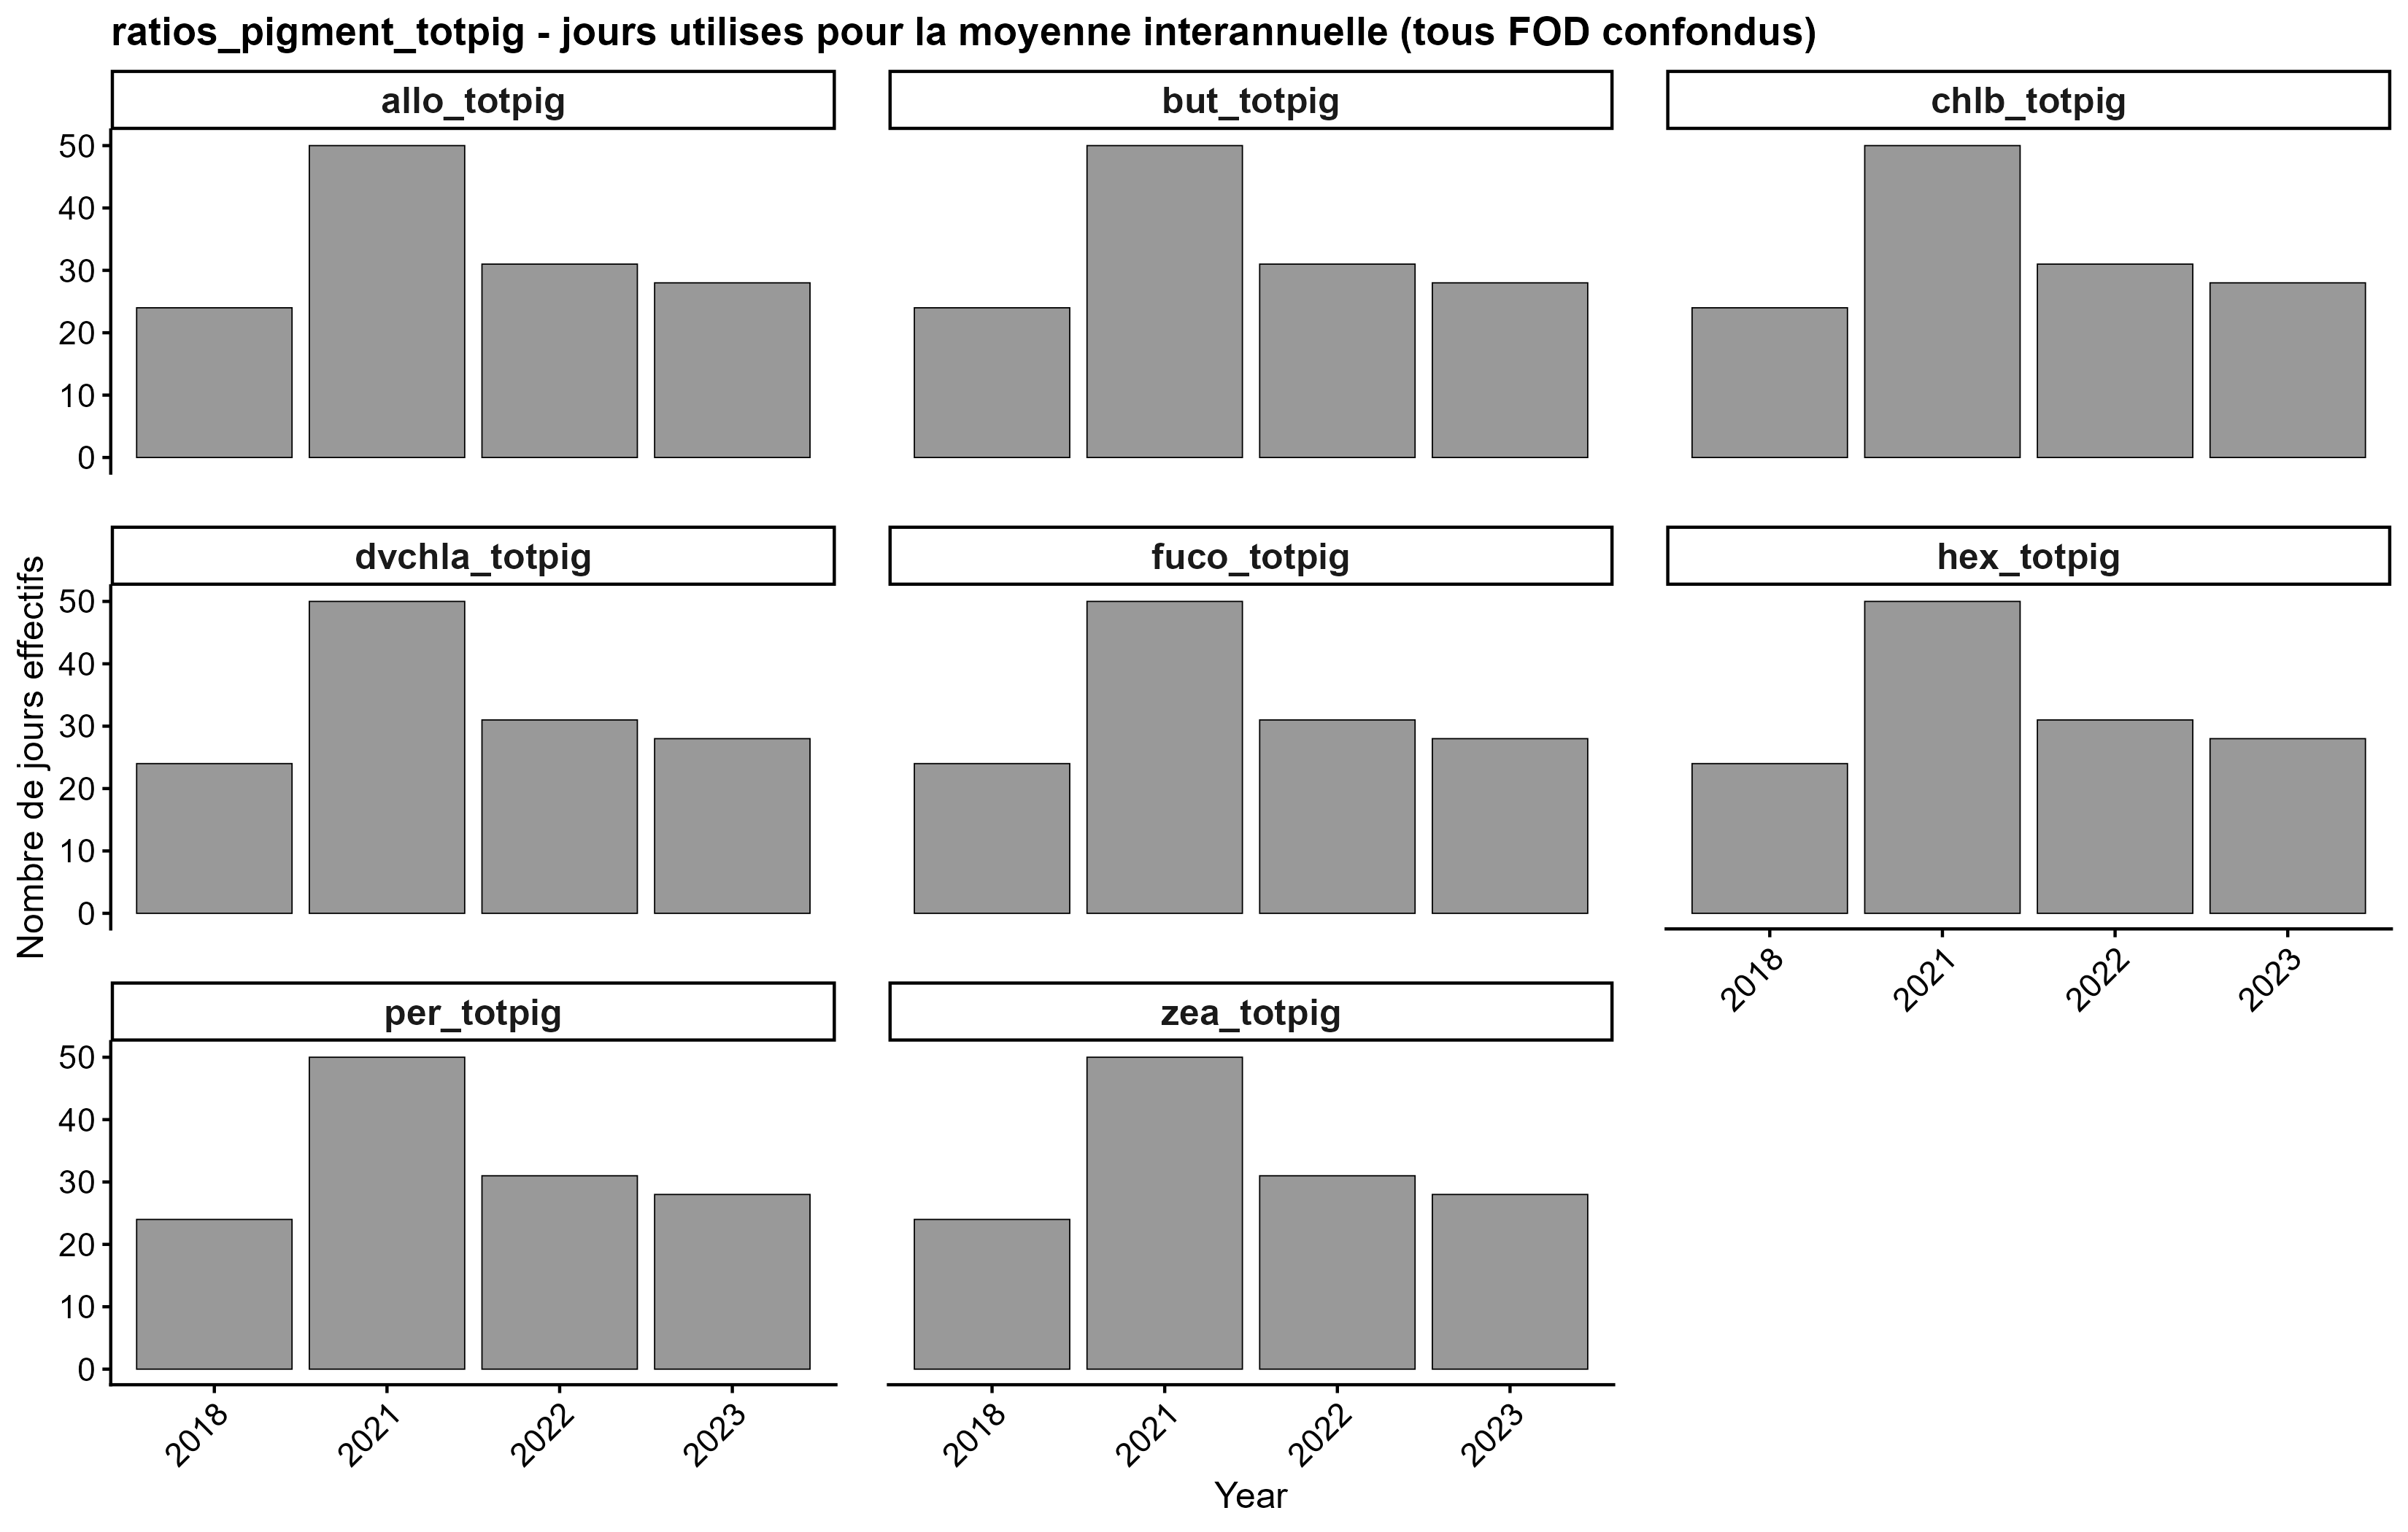
\includegraphics[width=0.6\textwidth]{images/05_annexes/04_resultats/01_distrib_ftle_nasc_ratio_chla/n_days_to_compute_distribs_ftle_nasc_pigs/ndays_interannual_ratios_pigment_totpig}
				\caption{Nombre de données effectives pour le calcul des distributions de la contribution de chaque pigment photosynthétique (2018, 2021, 2022, 2023) en période estivale sur la région étudiée du SO ([45, 90]°E, [30, 60]°S).}
				\label{fig:ndaysinterannualratiospigmenttotpig}
			\end{figure}
			\begin{figure}[H]
				\centering
				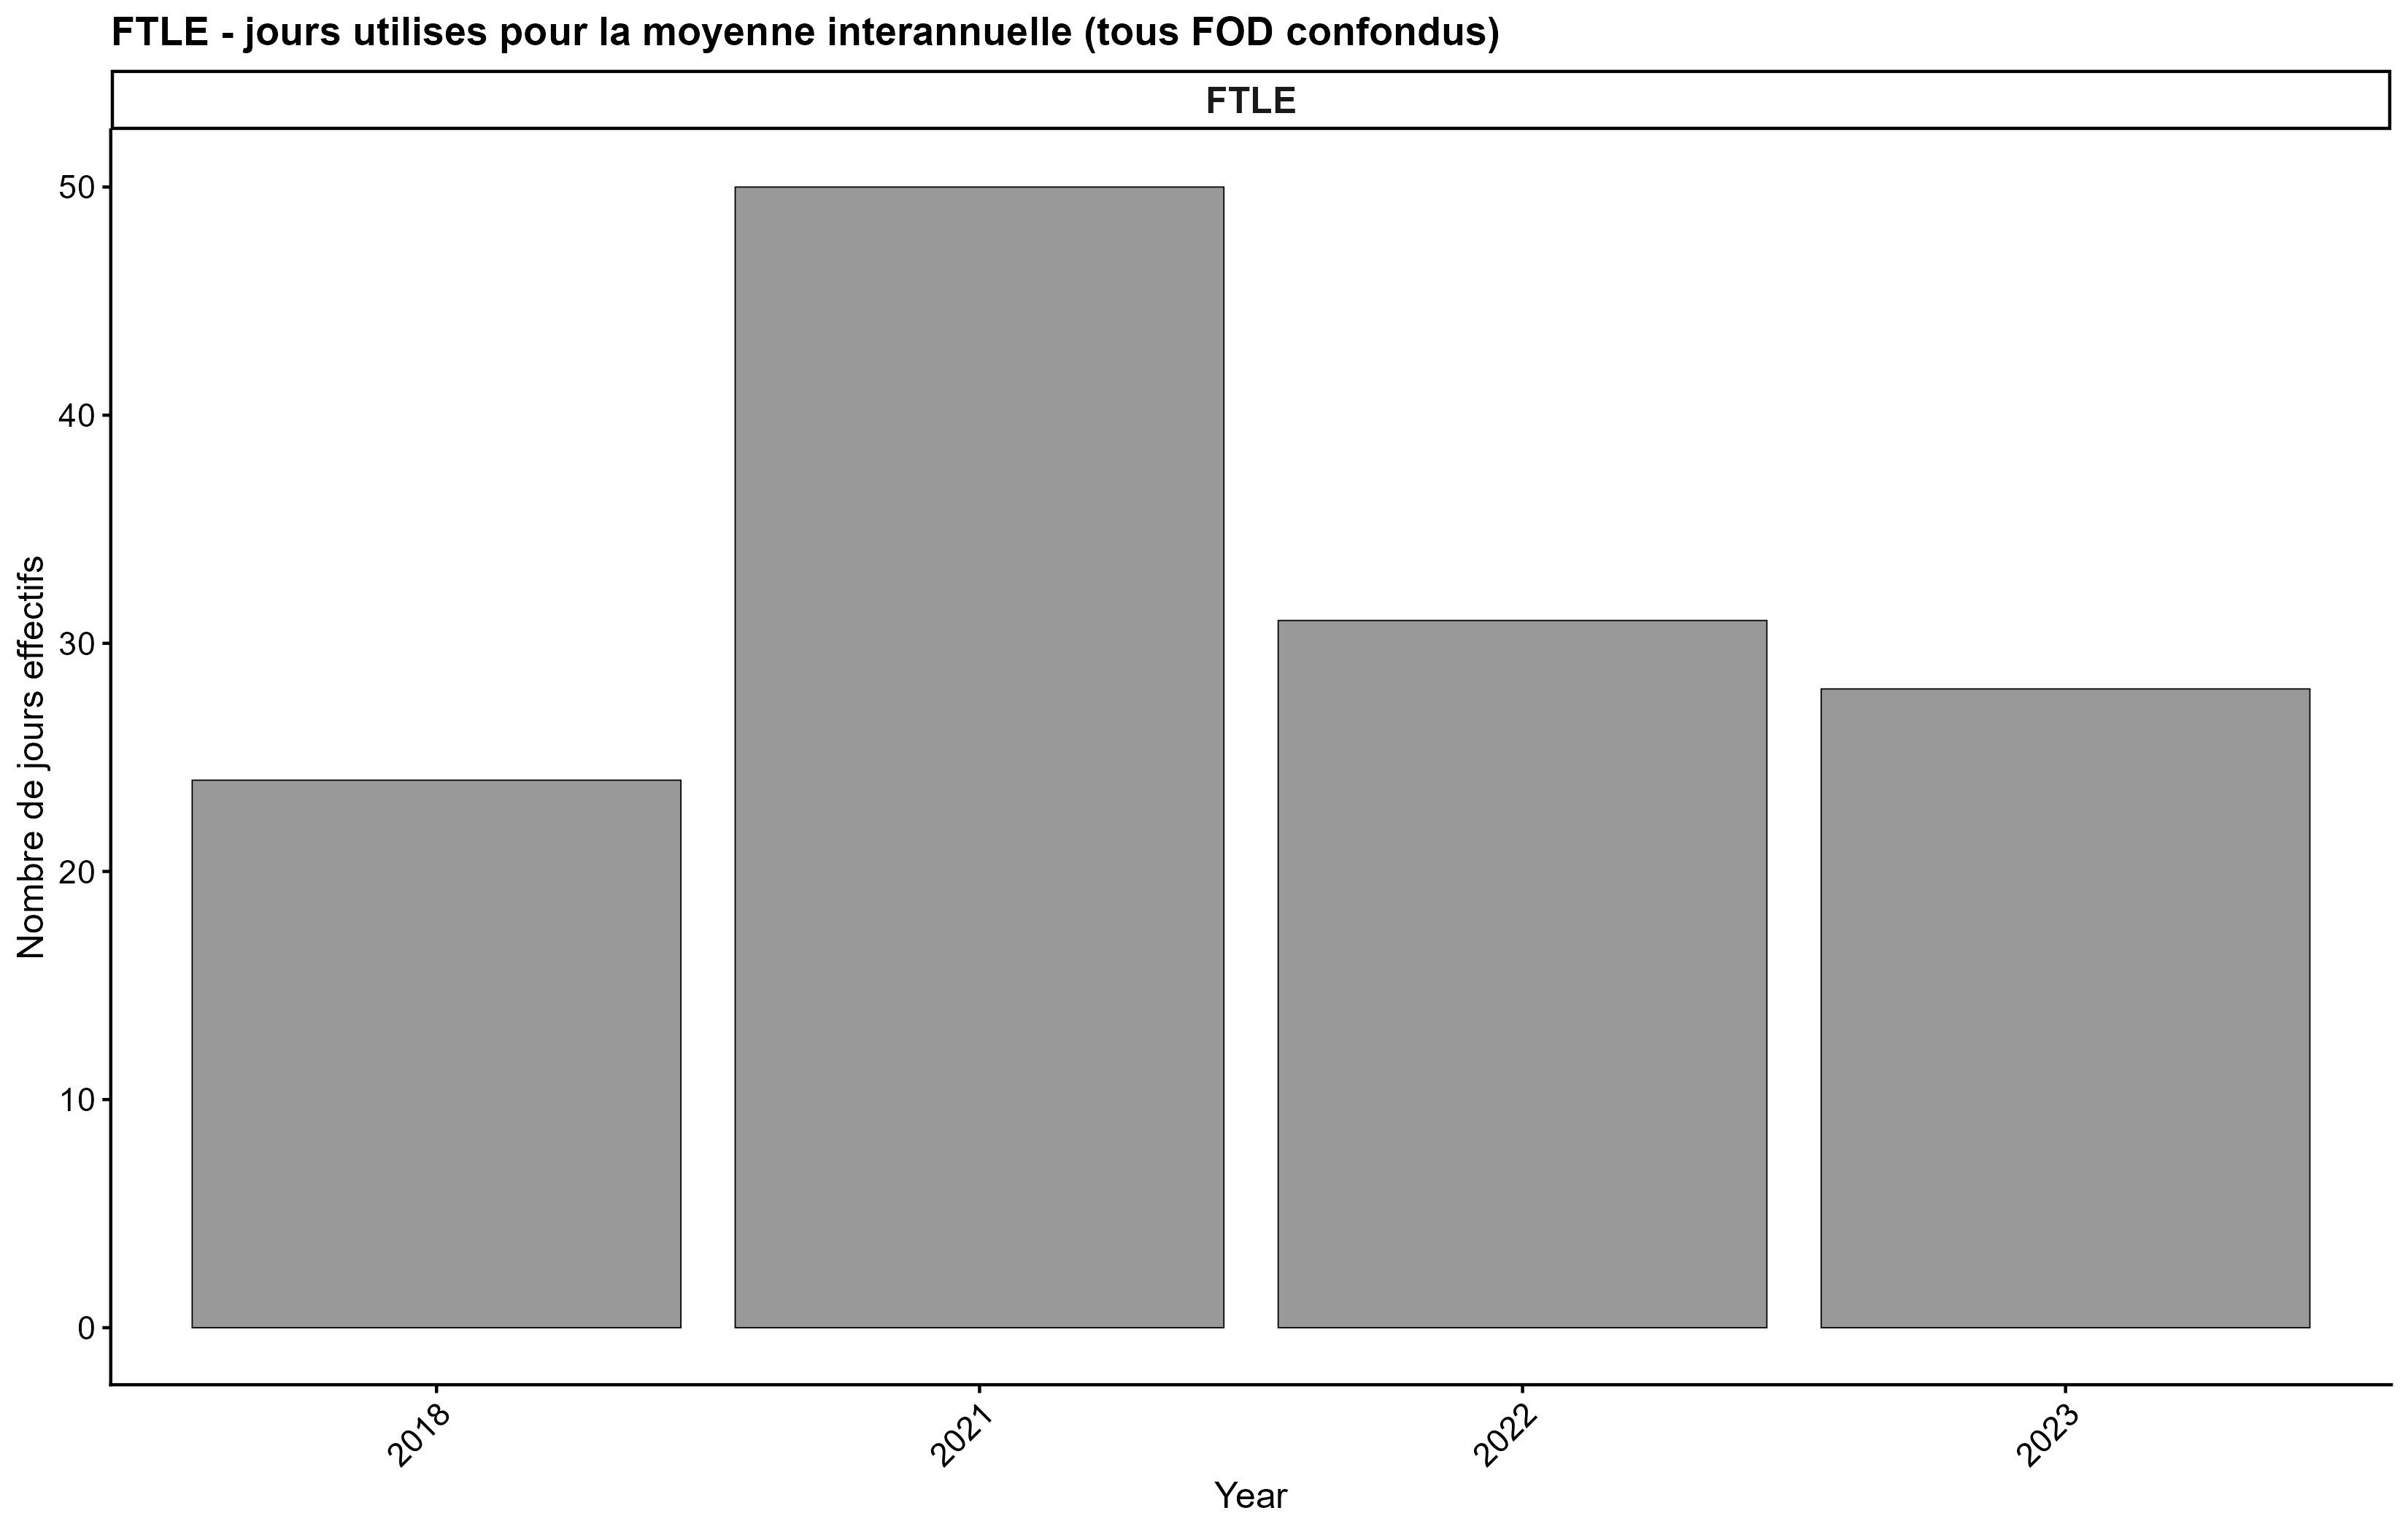
\includegraphics[width=0.6\textwidth]{images/05_annexes/04_resultats/01_distrib_ftle_nasc_ratio_chla/n_days_to_compute_distribs_ftle_nasc_pigs/ndays_interannual_FTLE}
				\caption{Nombre de données effectives pour le calcul des Finite Time Lyapunov Exponent (FTLE) (2018, 2021, 2022, 2023) en période estivale sur la région étudiée du SO ([45, 90]°E, [30, 60]°S).}
				\label{fig:ndaysinterannualftle}
			\end{figure}
			\begin{figure}[H]
				\centering
				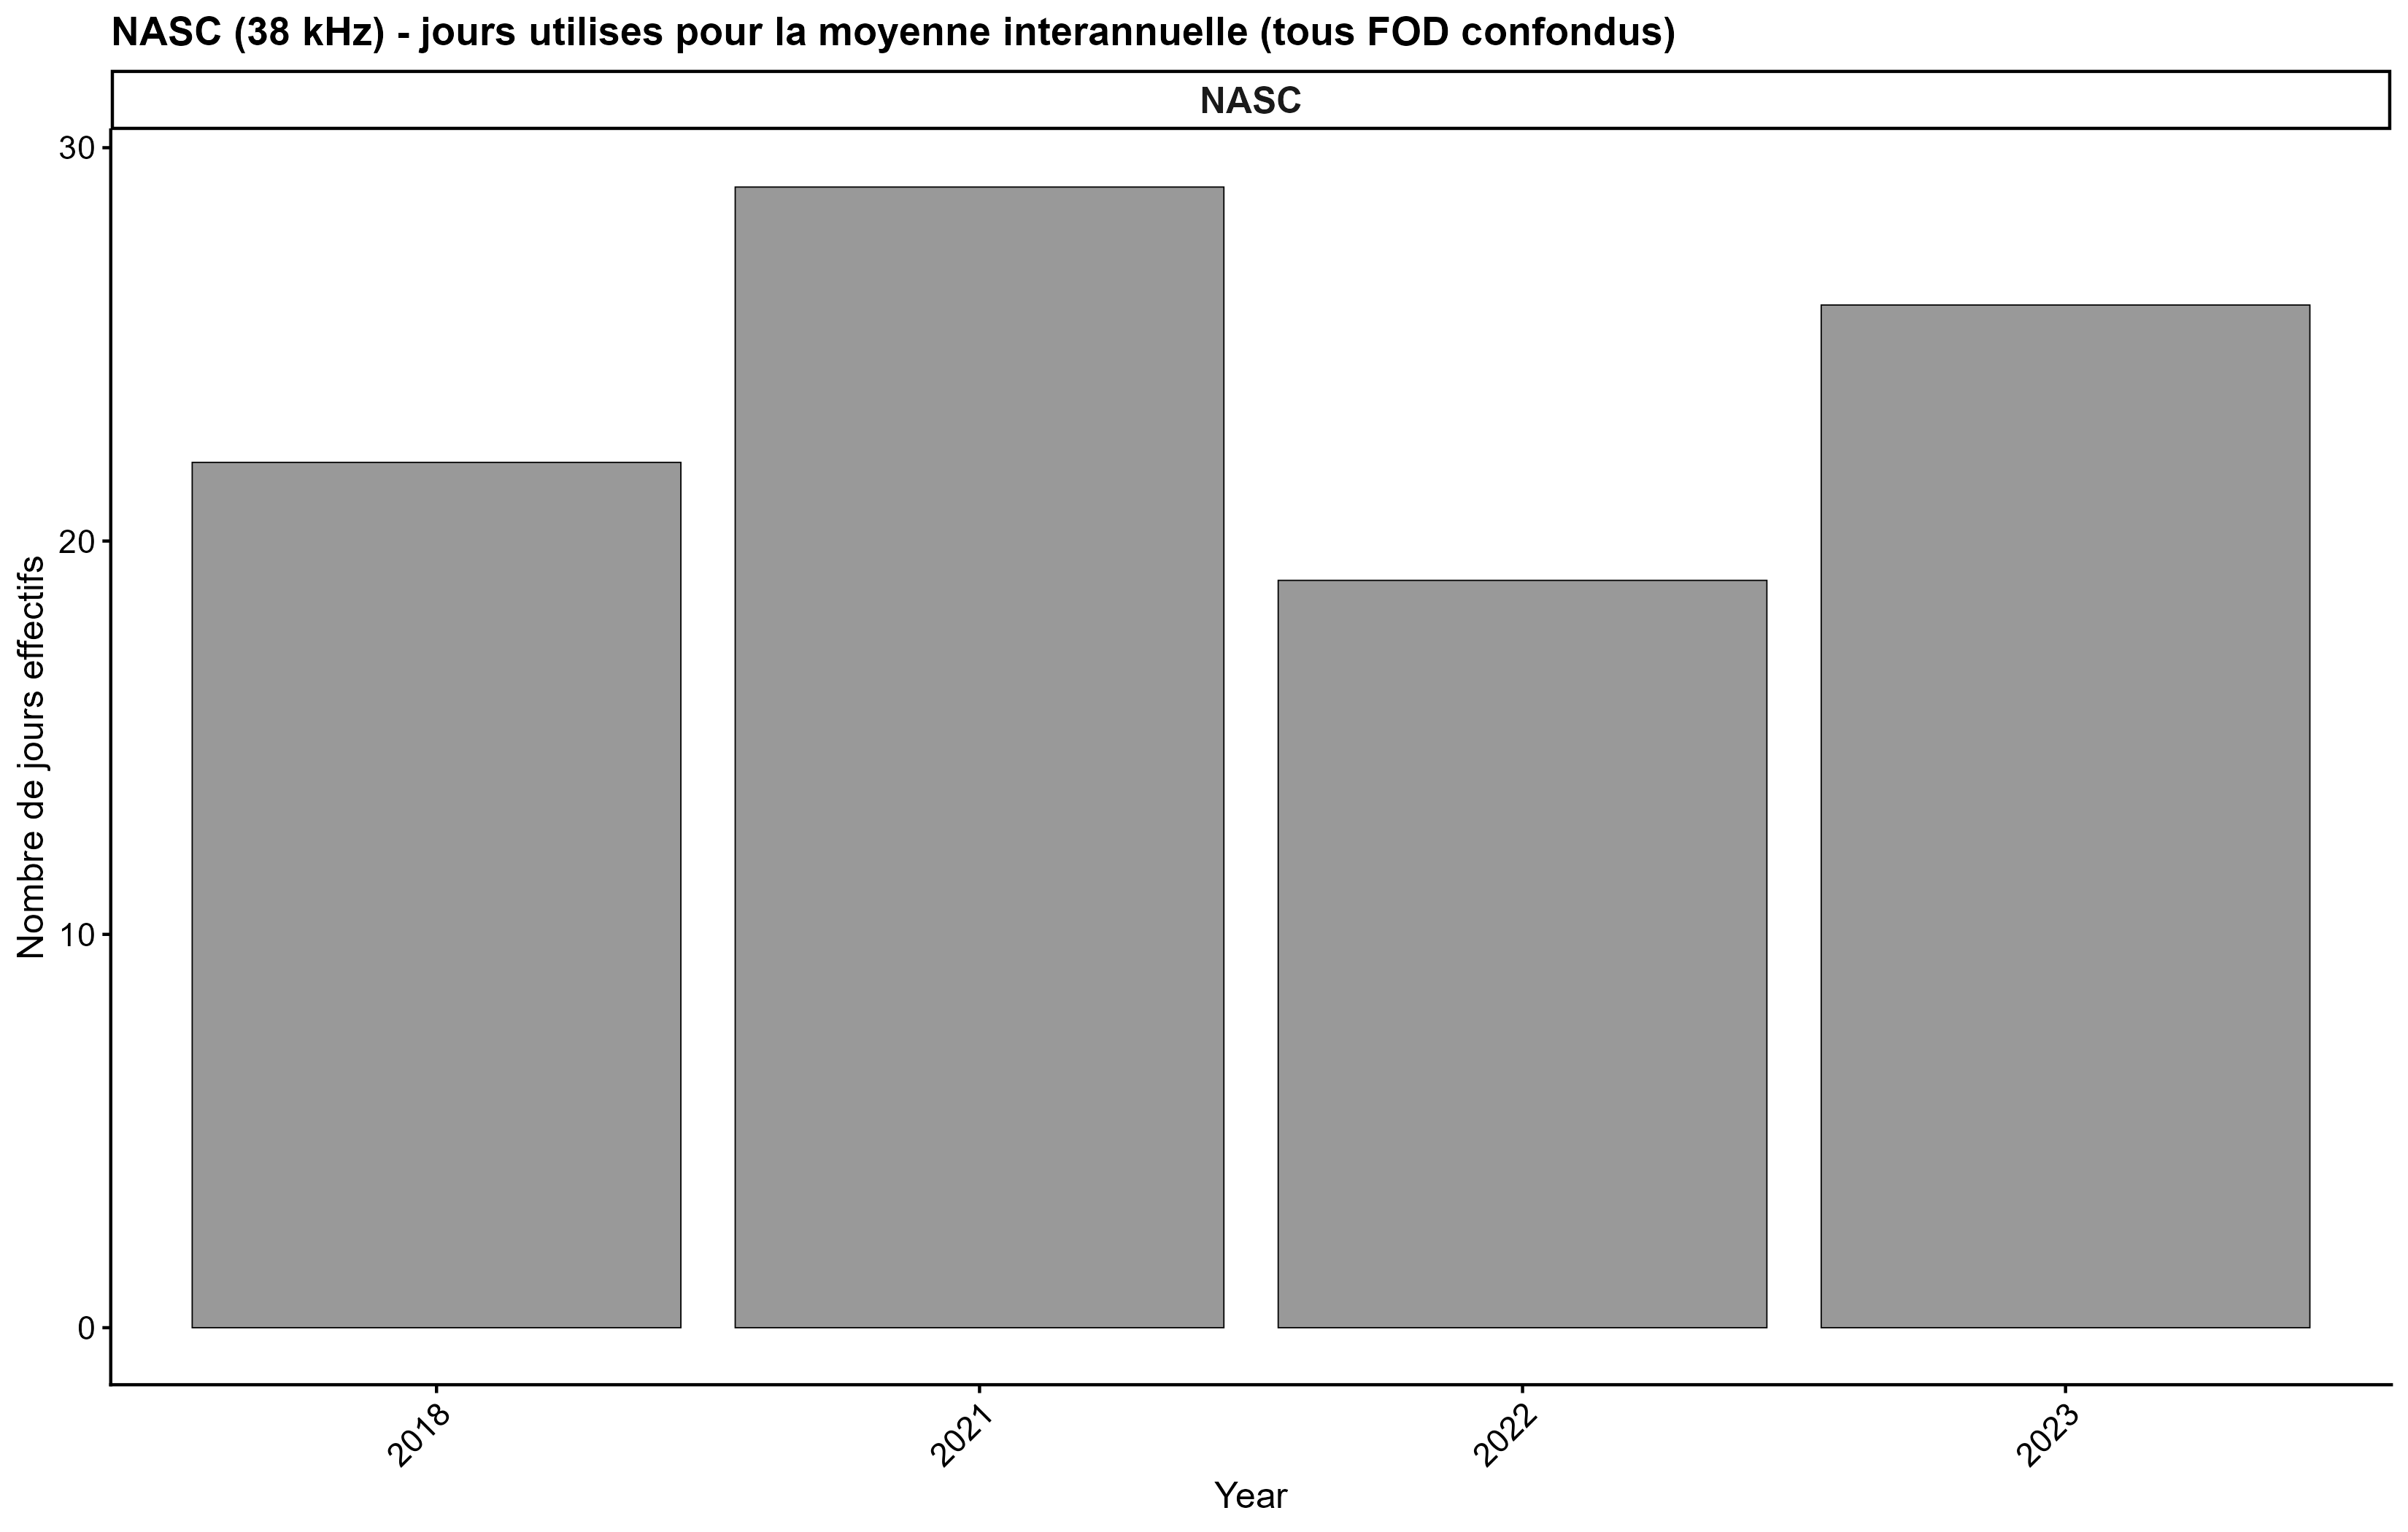
\includegraphics[width=0.6\textwidth]{images/05_annexes/04_resultats/01_distrib_ftle_nasc_ratio_chla/n_days_to_compute_distribs_ftle_nasc_pigs/ndays_interannual_NASC__38_kHz_}
				\caption{Nombre de données effectives pour le calcul des distributions de NASC (38kHz) (2018, 2021, 2022, 2023) en période estivale sur la région étudiée du SO ([45, 90]°E, [30, 60]°S).}
				\label{fig:ndaysinterannualnasc38khz}
			\end{figure}
			\begin{figure}[H]
				\centering
				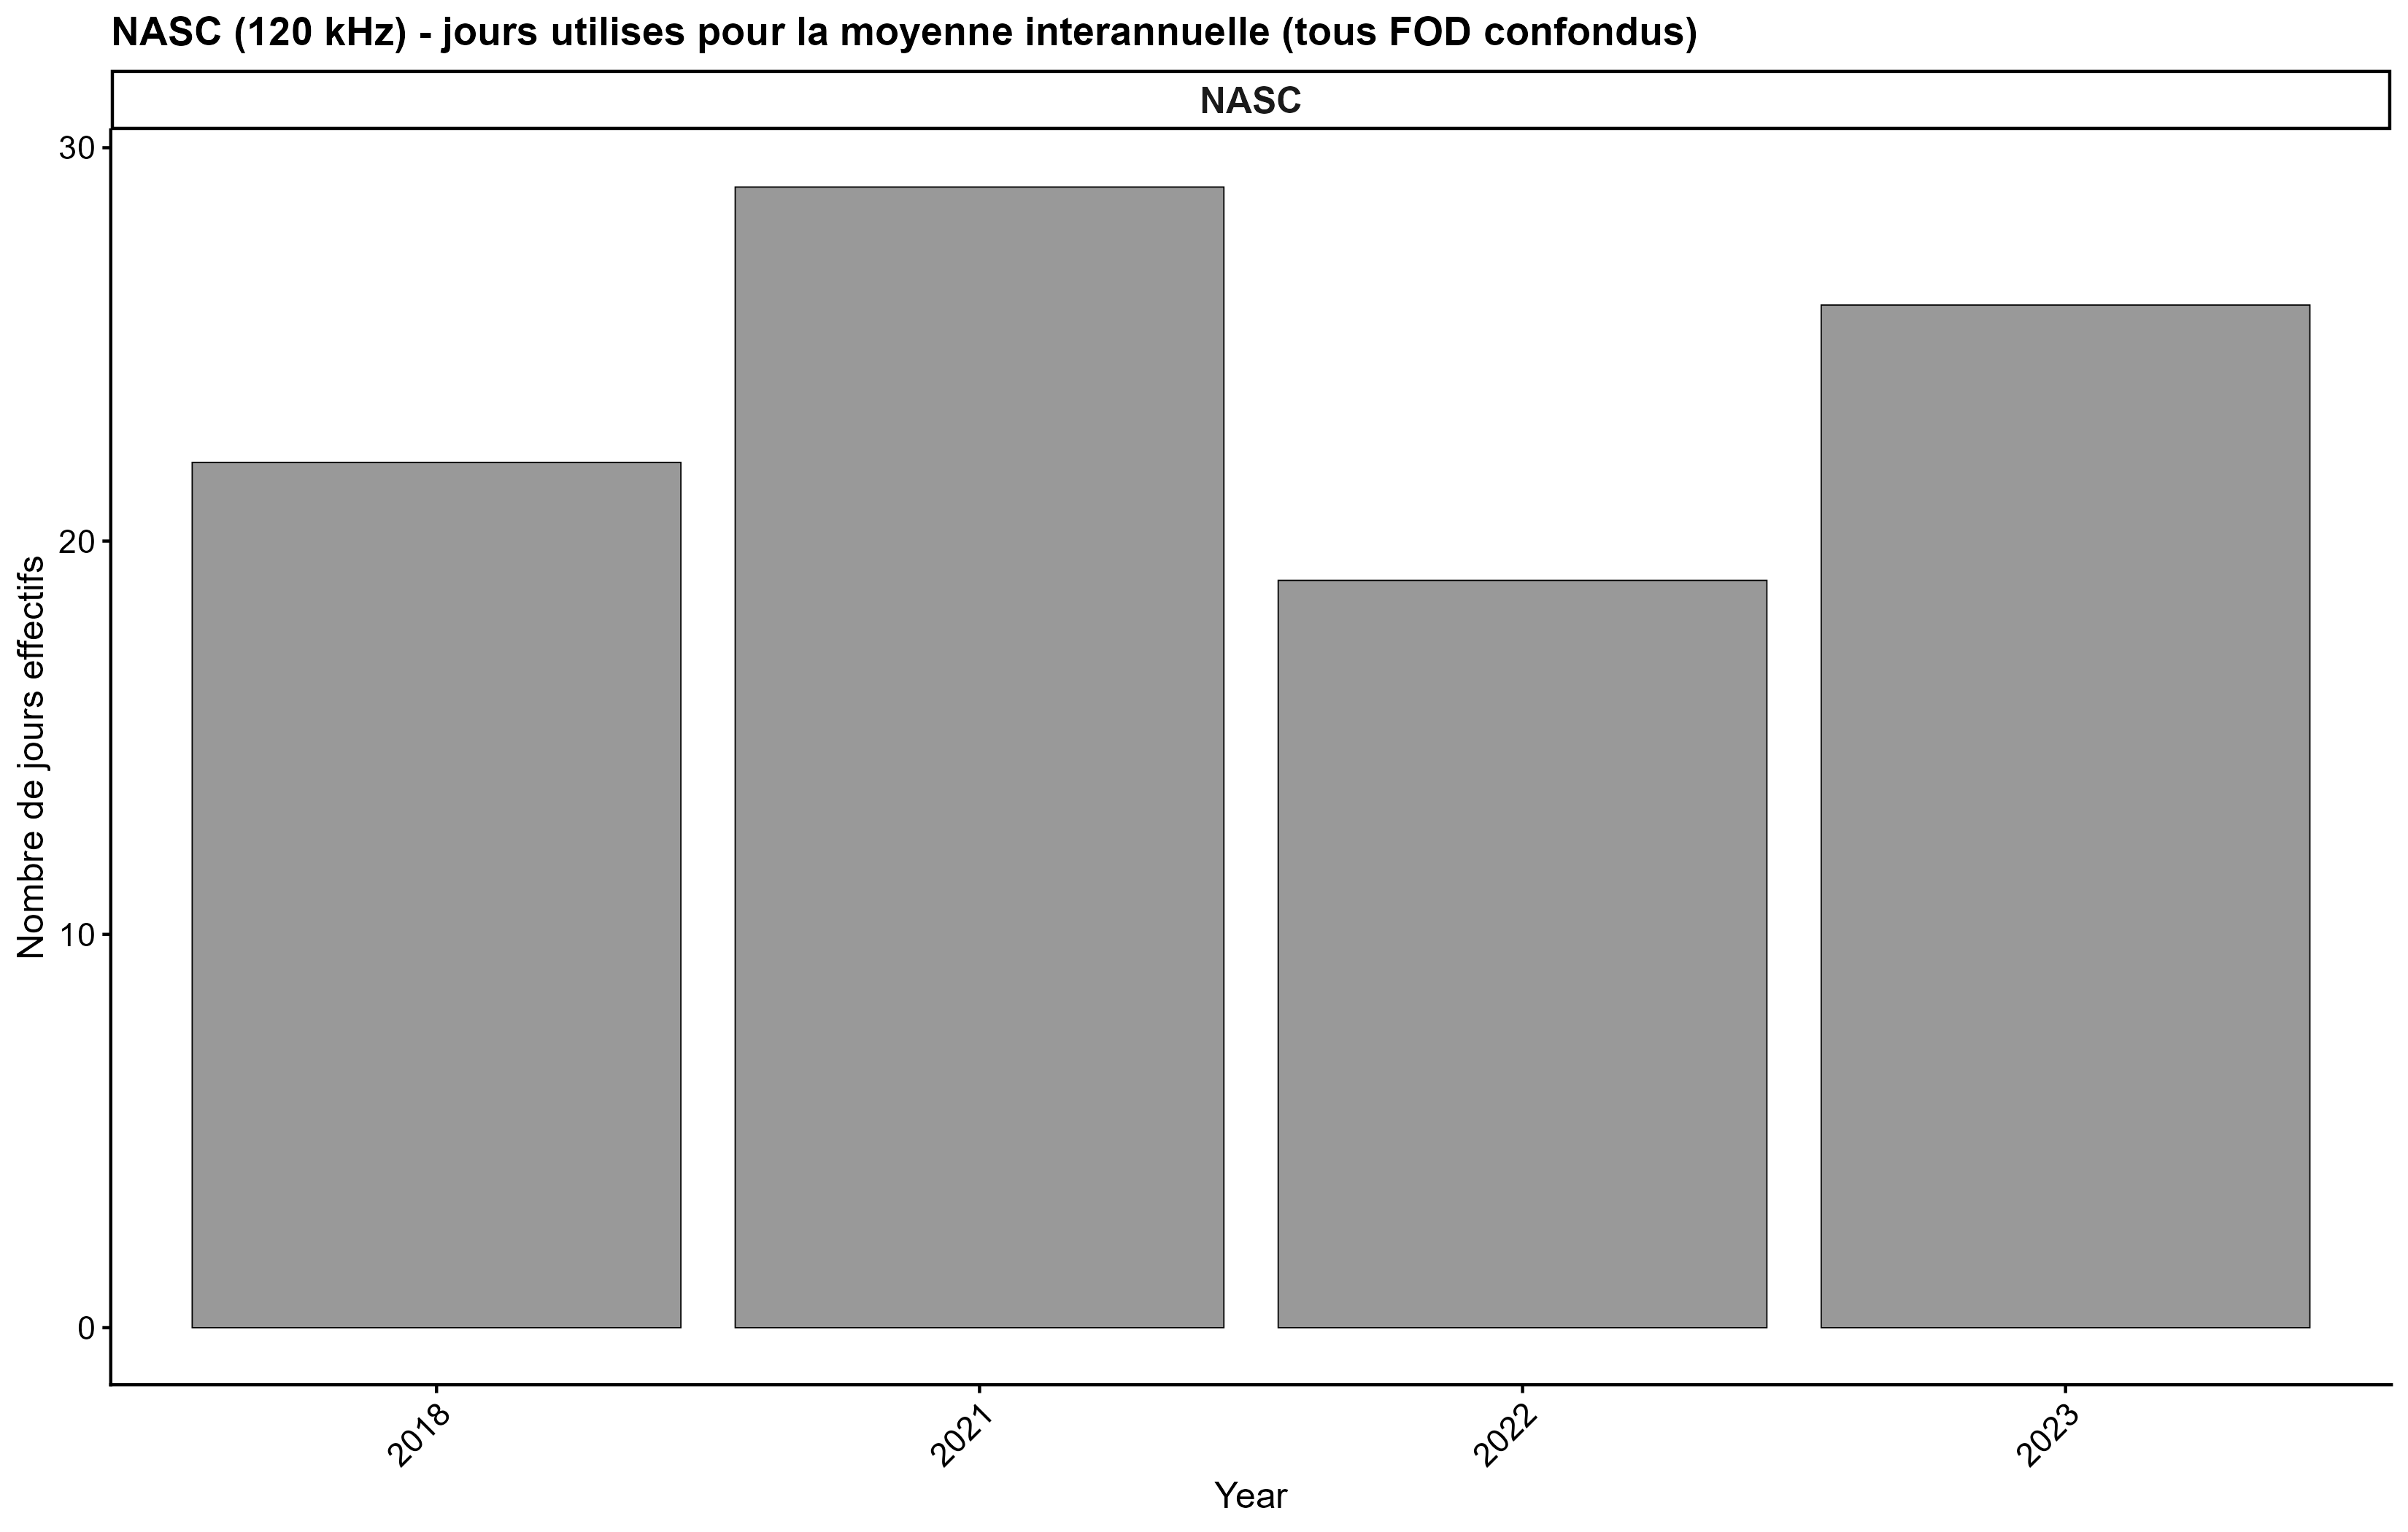
\includegraphics[width=0.6\textwidth]{images/05_annexes/04_resultats/01_distrib_ftle_nasc_ratio_chla/n_days_to_compute_distribs_ftle_nasc_pigs/ndays_interannual_NASC__120_kHz_}
				\caption{Nombre de données effectives pour le calcul des distributions de NASC (120 kHz) (2018, 2021, 2022, 2023) en période estivale sur la région étudiée du SO ([45, 90]°E, [30, 60]°S).}
				\label{fig:ndaysinterannualnasc120khz}
			\end{figure}
			
		\subsection{Distributions par FOD}
		\begin{figure}[H]
			\centering
			
			% --- Rangée 1 ---
			\begin{subfigure}[t]{0.48\textwidth}
				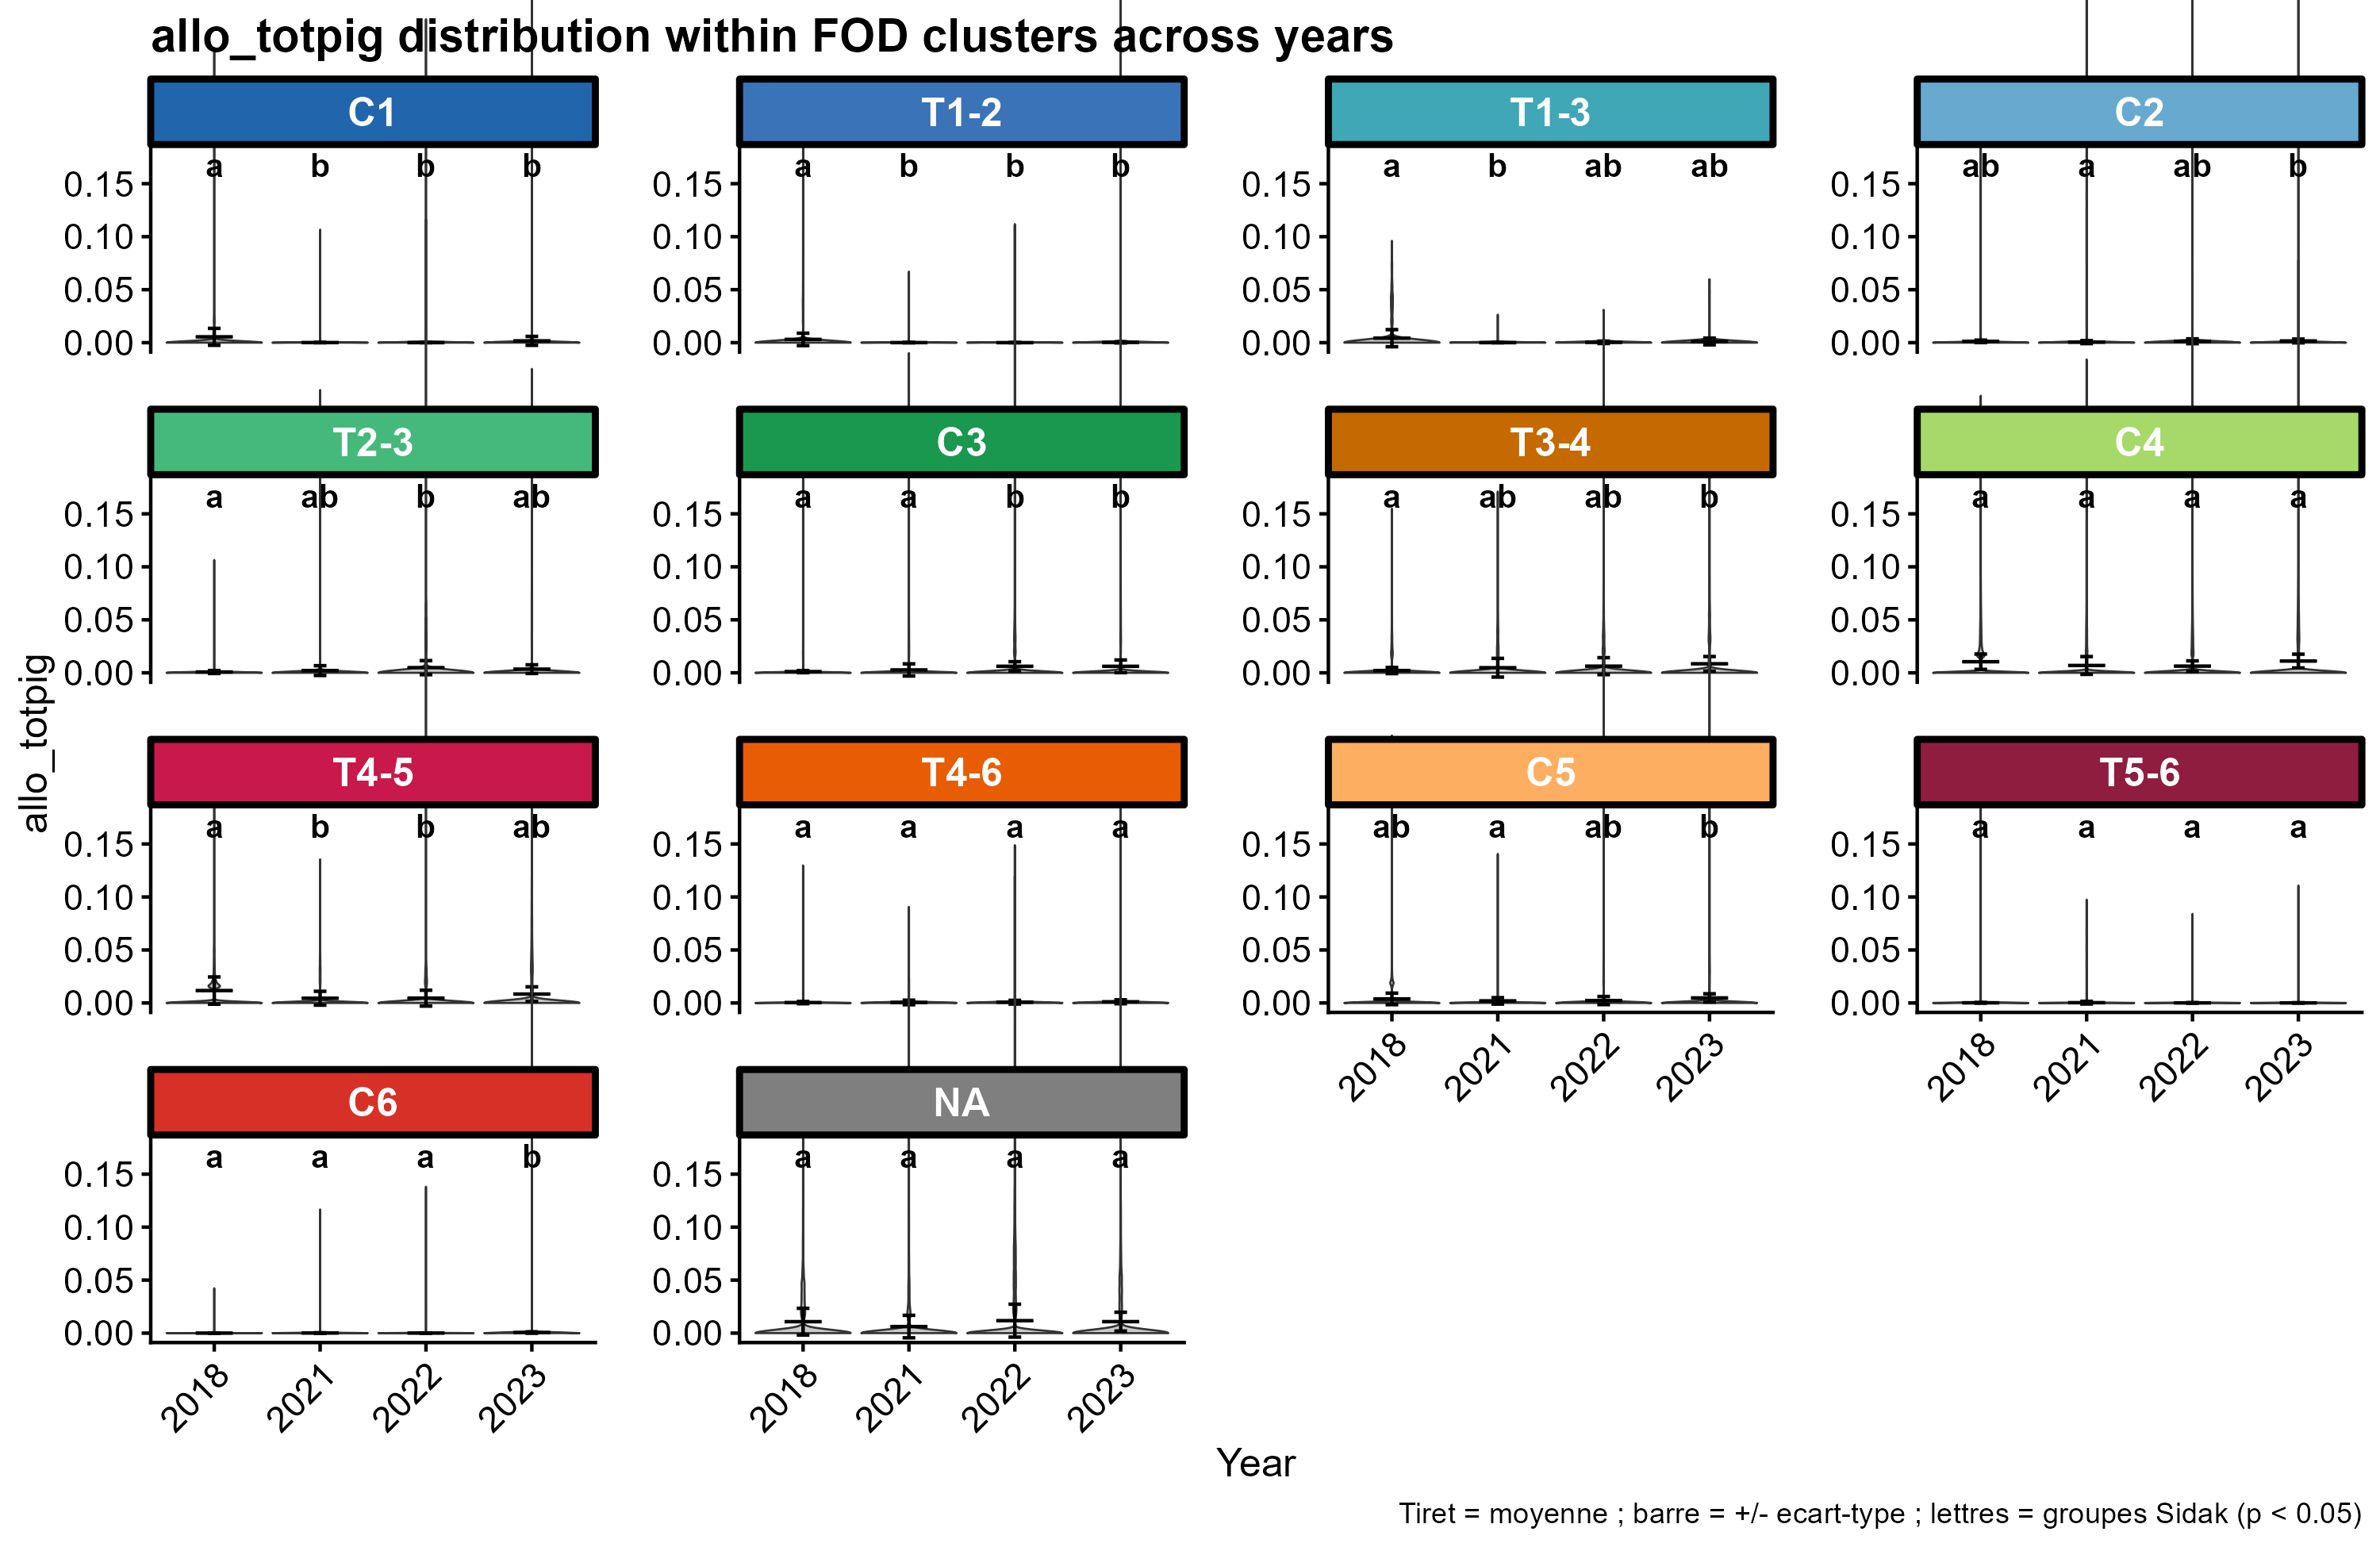
\includegraphics[width=\textwidth]{images/05_annexes/04_resultats/distrib_ftle_nasc_pig_per_fod/violin_allo_totpig}
				\caption{Alloxanthine / $\Sigma$pigments}
			\end{subfigure}
			\hfill
			\begin{subfigure}[t]{0.48\textwidth}
				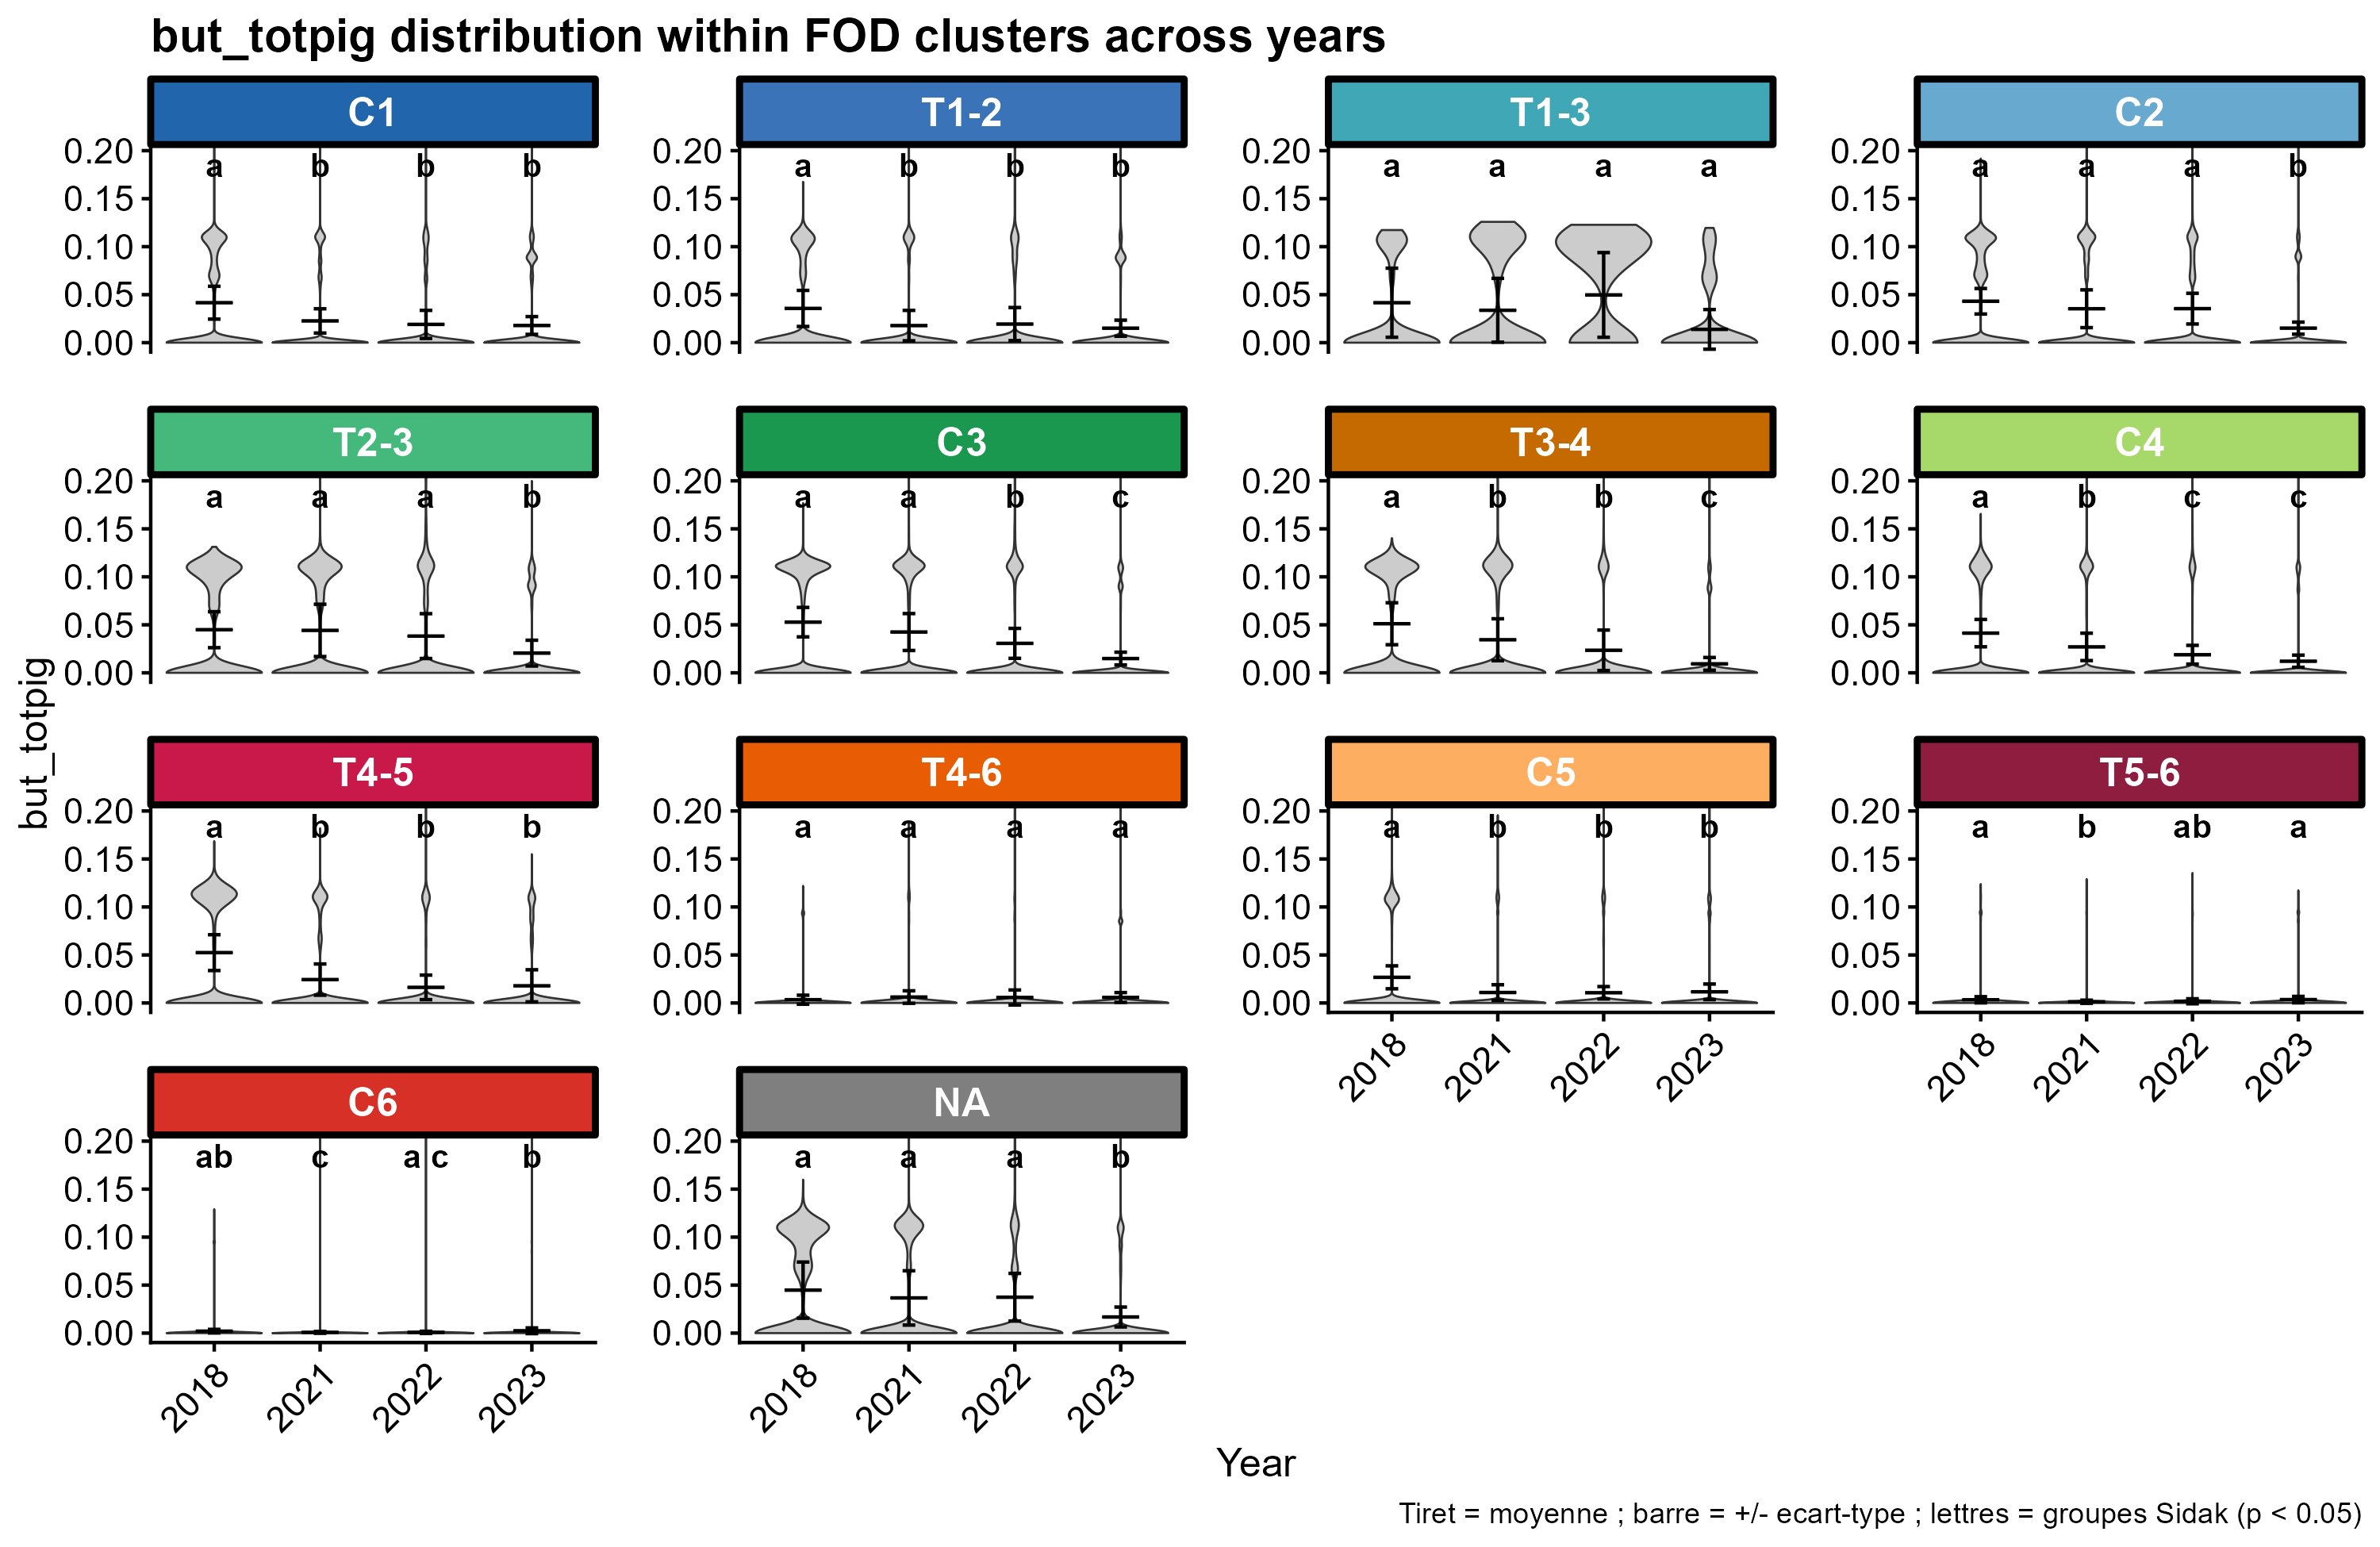
\includegraphics[width=\textwidth]{images/05_annexes/04_resultats/distrib_ftle_nasc_pig_per_fod/violin_but_totpig}
				\caption{19'-Butanoyloxyfucoxanthine / $\Sigma$pigments}
			\end{subfigure}
			
			\vfill
			
			% --- Rangée 2 ---
			\begin{subfigure}[t]{0.48\textwidth}
				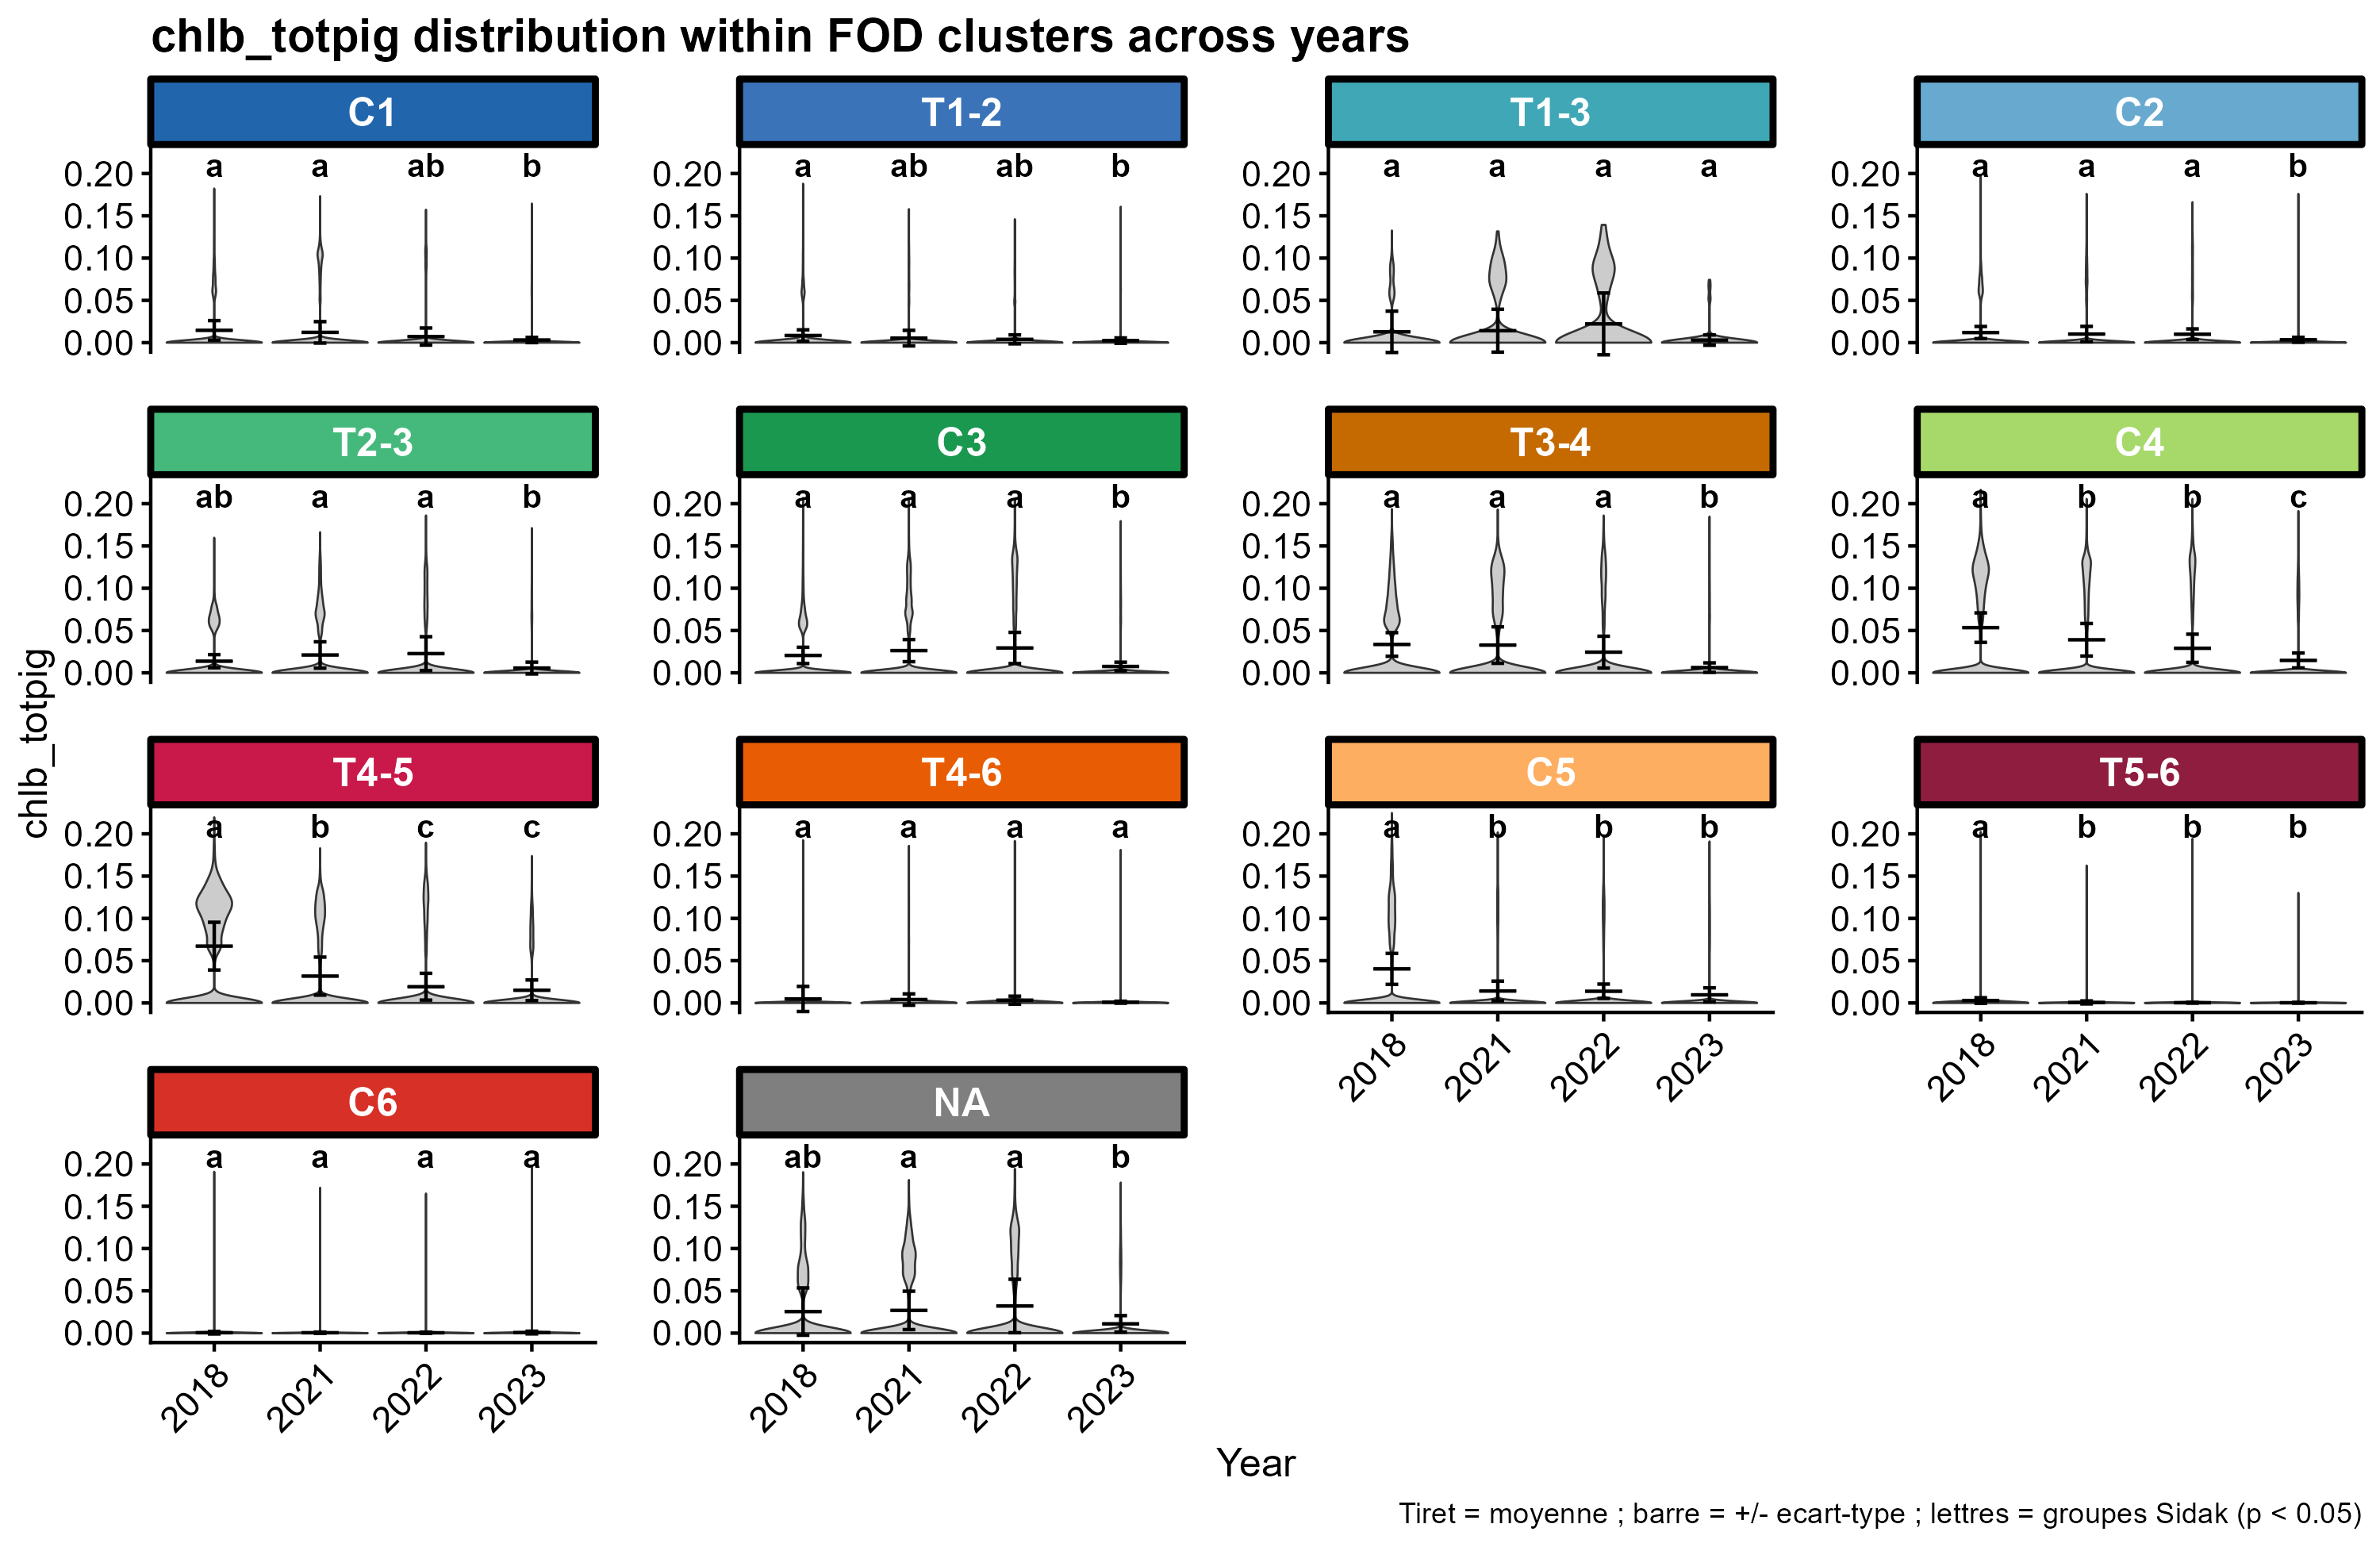
\includegraphics[width=\textwidth]{images/05_annexes/04_resultats/distrib_ftle_nasc_pig_per_fod/violin_chlb_totpig}
				\caption{Chlorophylle b / $\Sigma$pigments}
			\end{subfigure}
			\hfill
			\begin{subfigure}[t]{0.48\textwidth}
				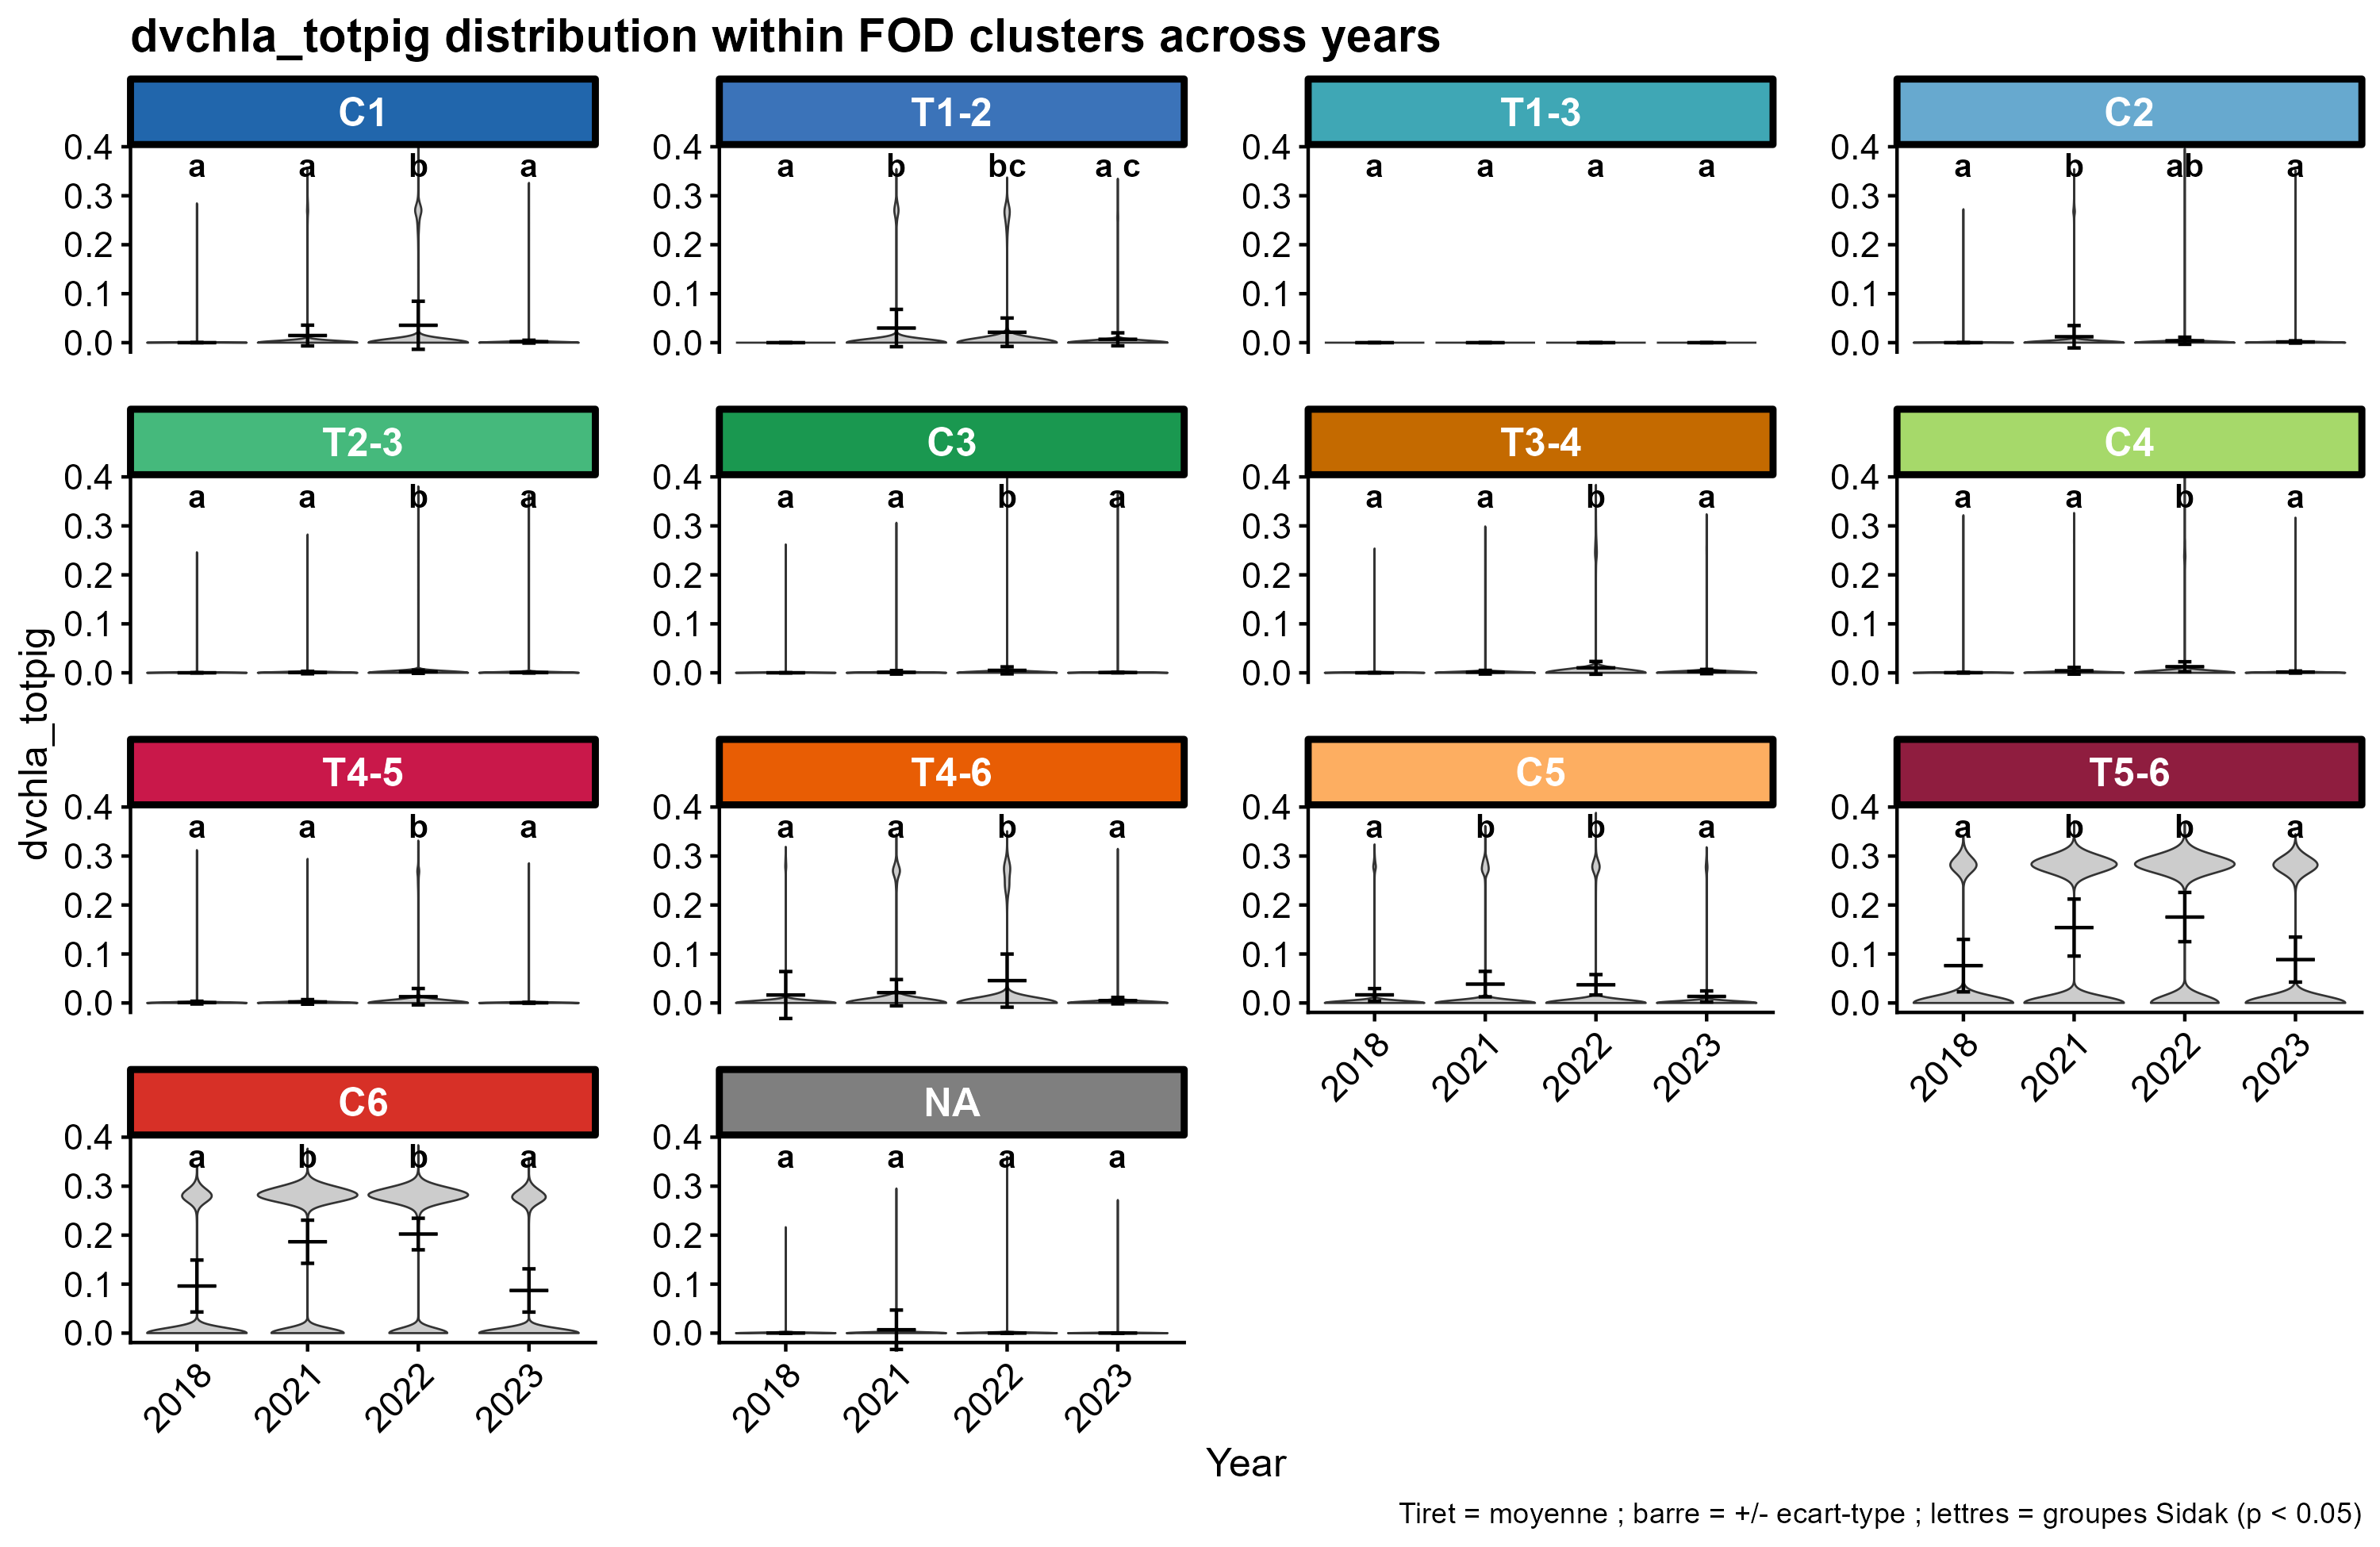
\includegraphics[width=\textwidth]{images/05_annexes/04_resultats/distrib_ftle_nasc_pig_per_fod/violin_dvchla_totpig}
				\caption{Divinyl-chlorophylle a / $\Sigma$pigments}
			\end{subfigure}
			
			\vfill
			
			% --- Rangée 3 ---
			\begin{subfigure}[t]{0.48\textwidth}
				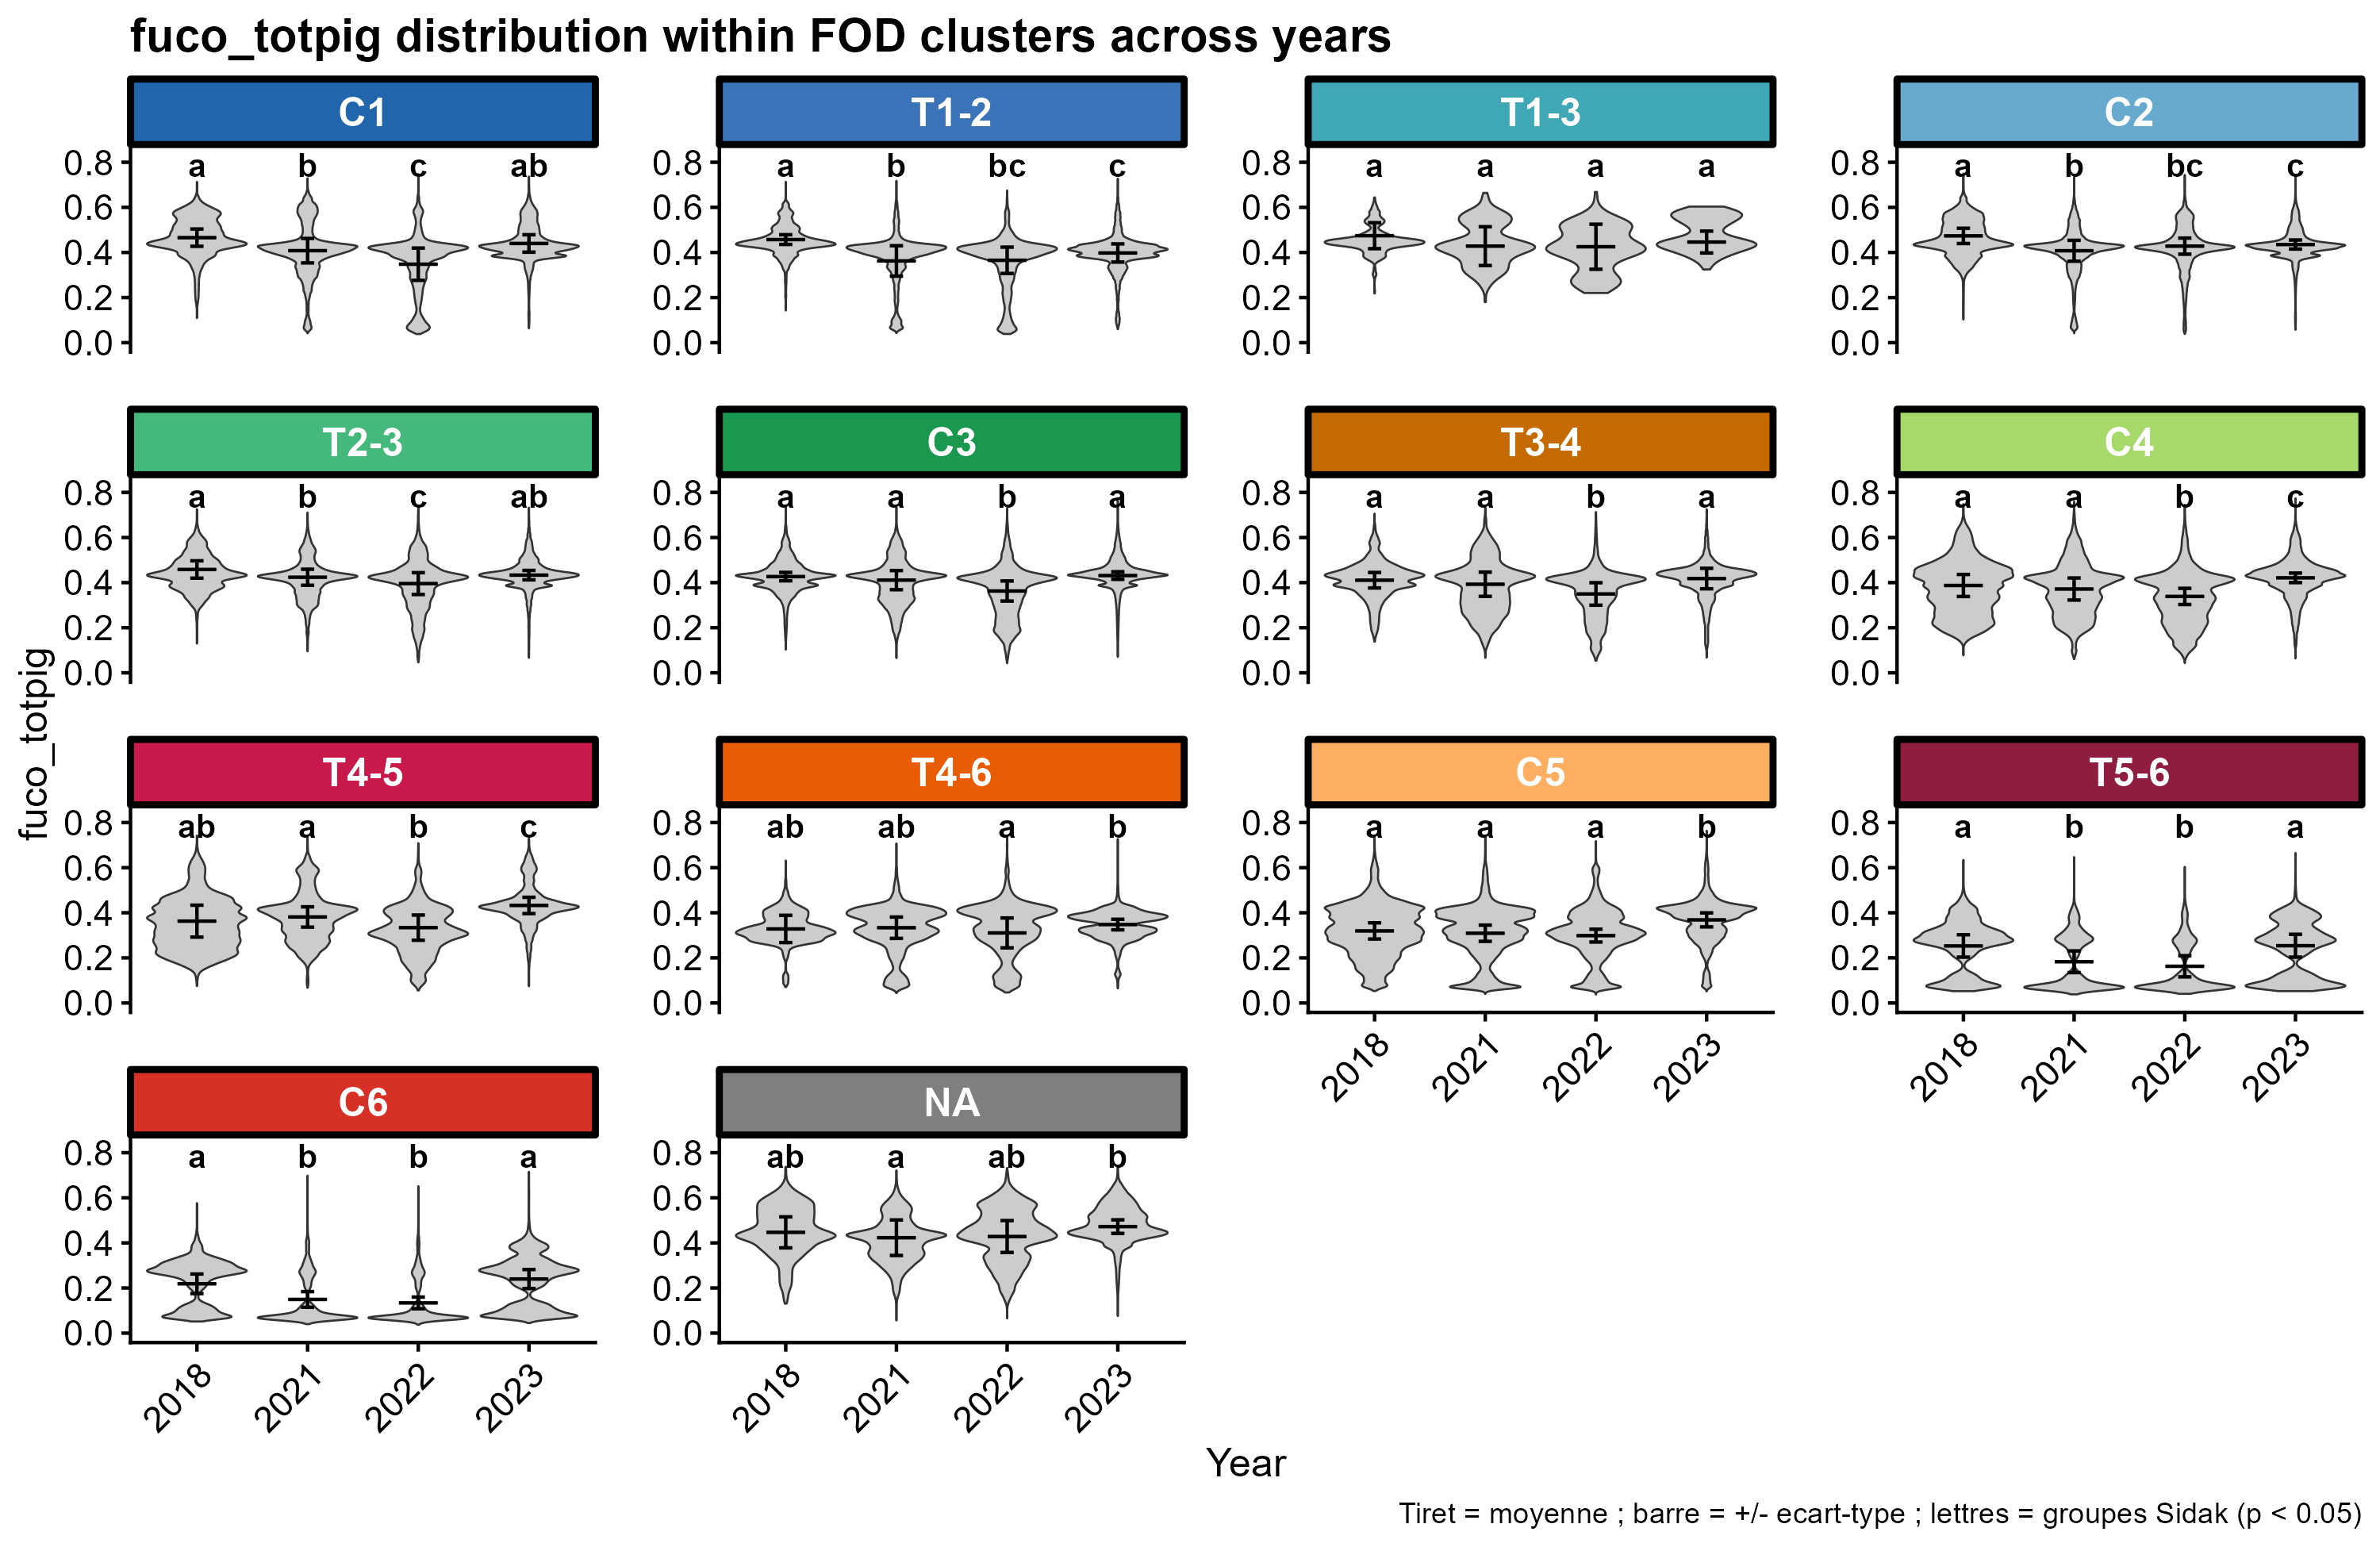
\includegraphics[width=\textwidth]{images/05_annexes/04_resultats/distrib_ftle_nasc_pig_per_fod/violin_fuco_totpig}
				\caption{Fucoxanthine / $\Sigma$pigments}
			\end{subfigure}
			\hfill
			\begin{subfigure}[t]{0.48\textwidth}
				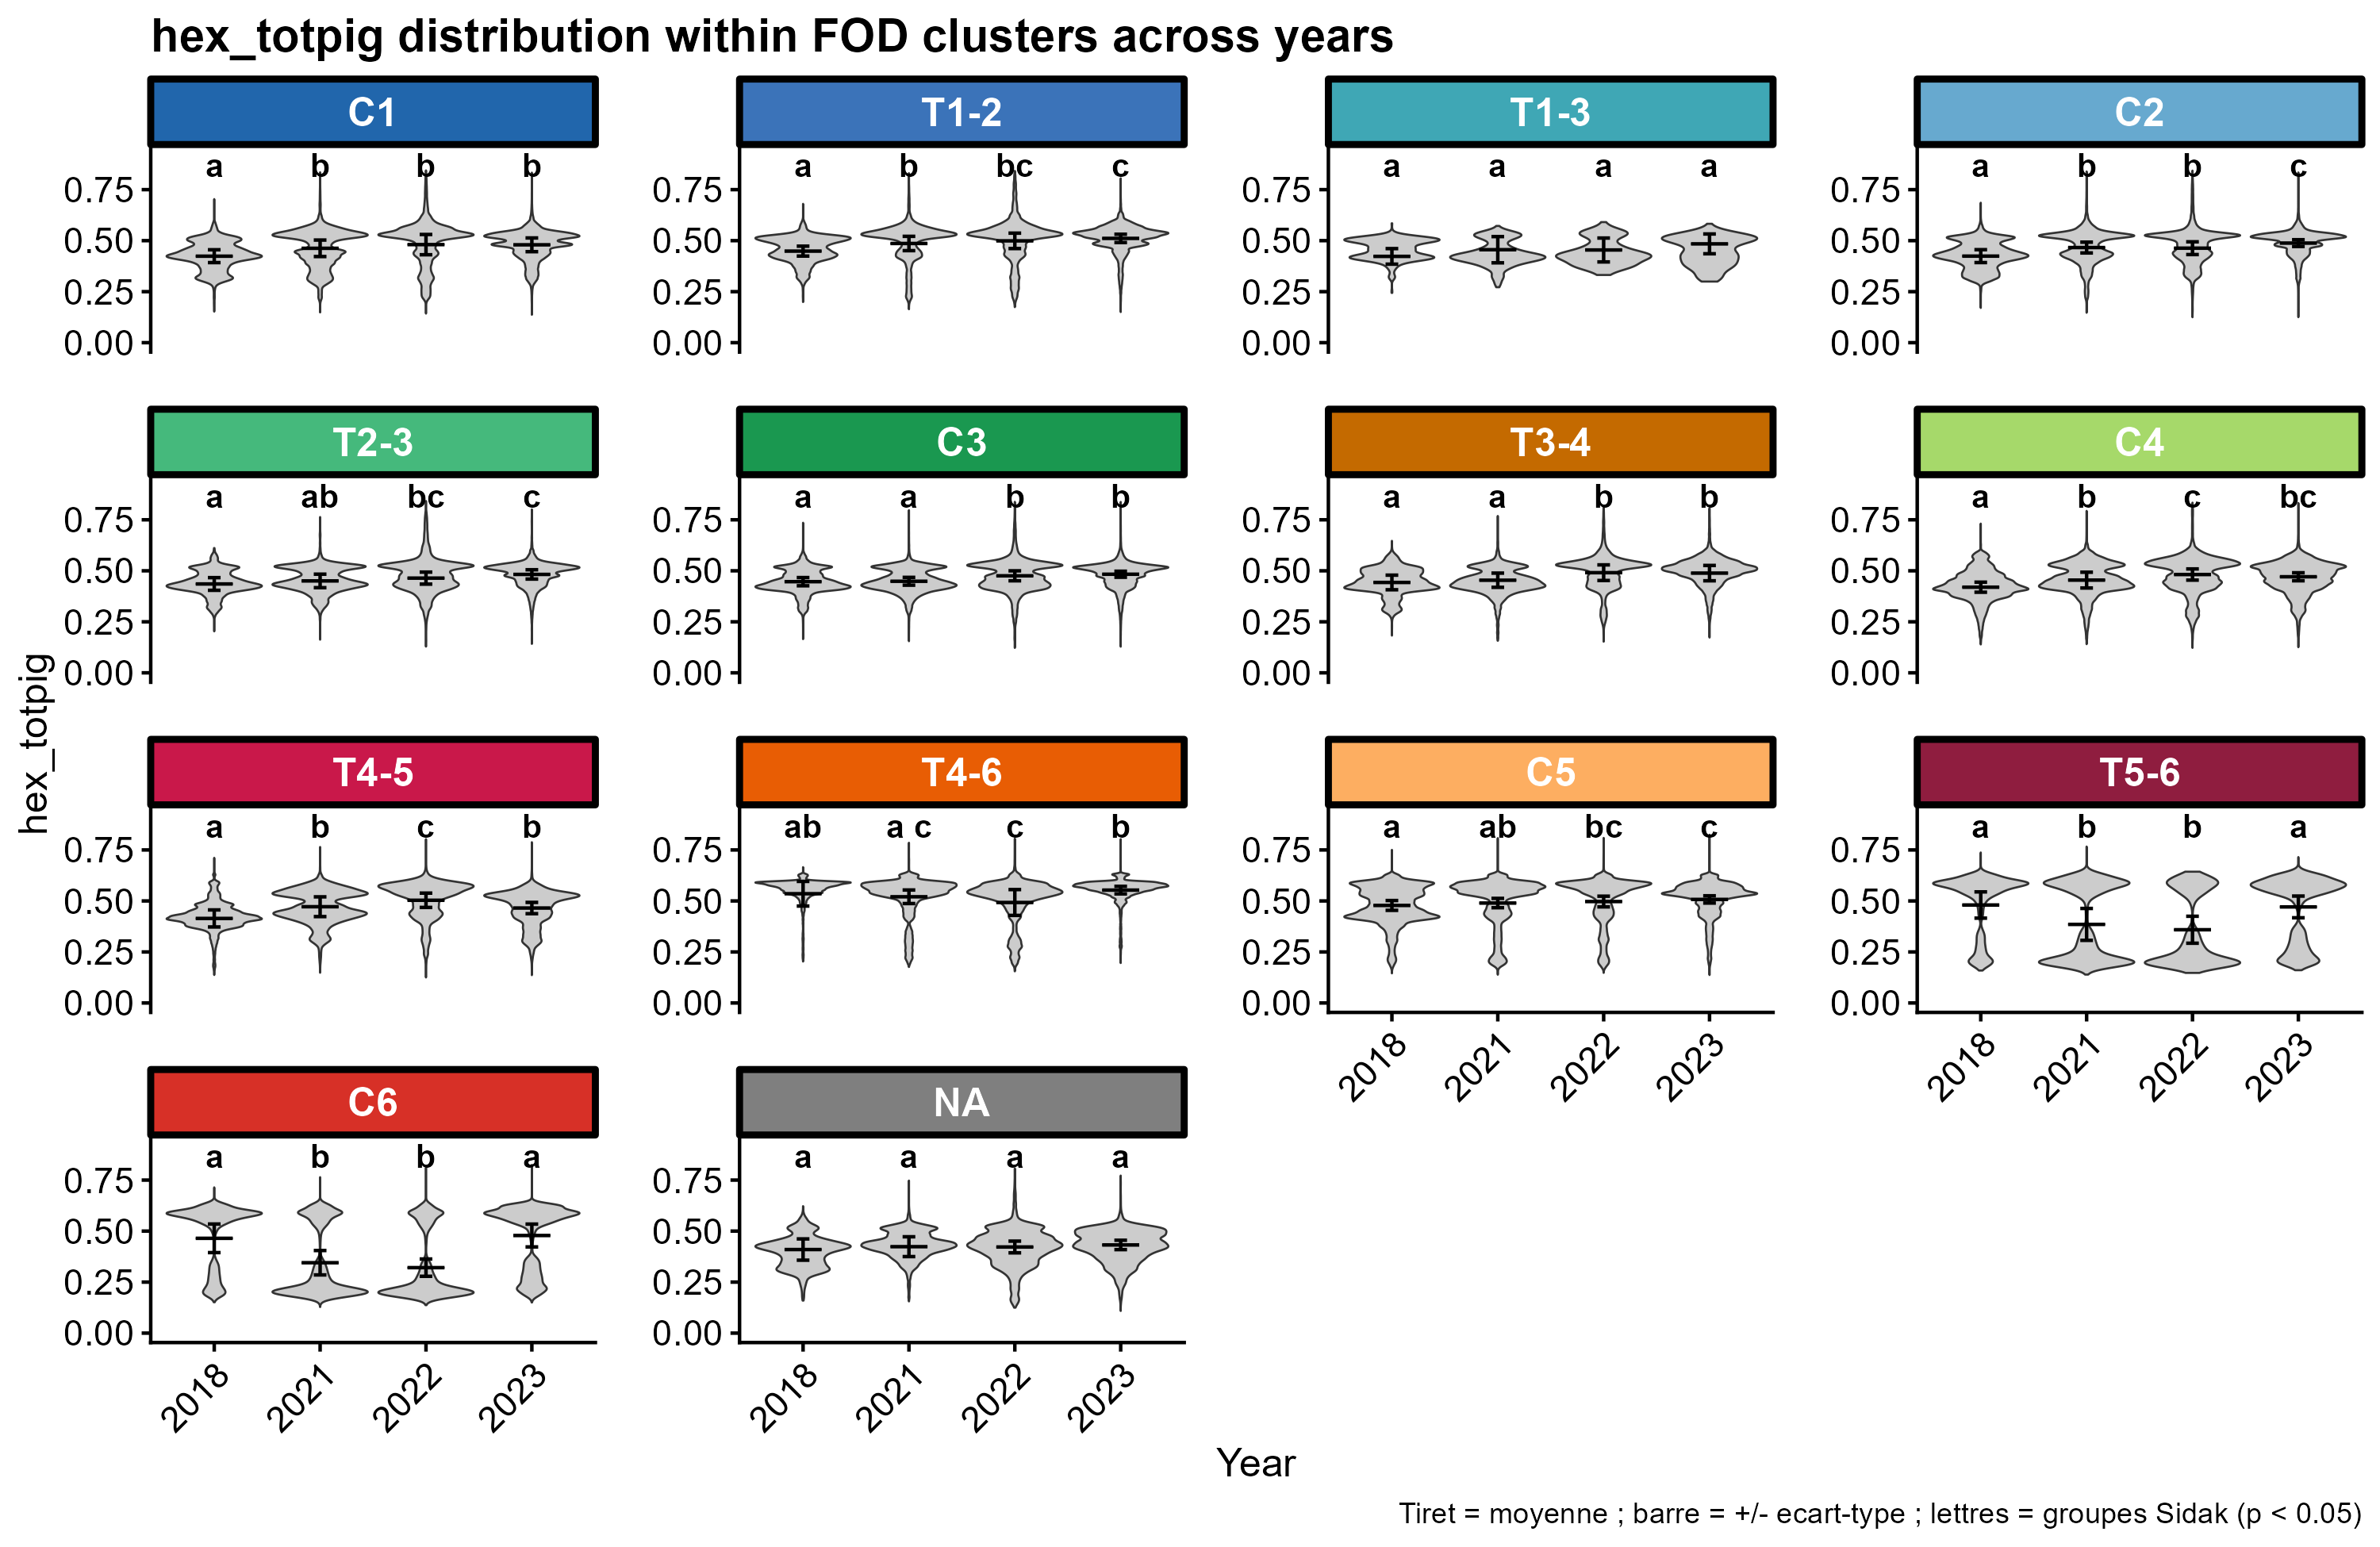
\includegraphics[width=\textwidth]{images/05_annexes/04_resultats/distrib_ftle_nasc_pig_per_fod/violin_hex_totpig}
				\caption{19'-Hexanoyloxyfucoxanthine / $\Sigma$pigments}
			\end{subfigure}
			
			\caption[Distributions inter-annuelles au sein des clusters FOD]{Distributions inter-annuelles (2018, 2021, 2022, 2023) des variables pigmentaires, du FTLE et acoustiques au sein des clusters FOD obtenus lors des campagnes océanographiques OBSAUSTRAL/THEMISTO. Les variables pigmentaires sont exprimées comme le rapport de chaque pigment accessoire à la somme des pigments (hors chlorophylle a).}
			\label{fig:annexe_violins_all}
		\end{figure}
		
		\begin{figure}[H]
			\ContinuedFloat
			\centering
			
			% --- Rangée 1 ---
			\begin{subfigure}[t]{0.48\textwidth}
				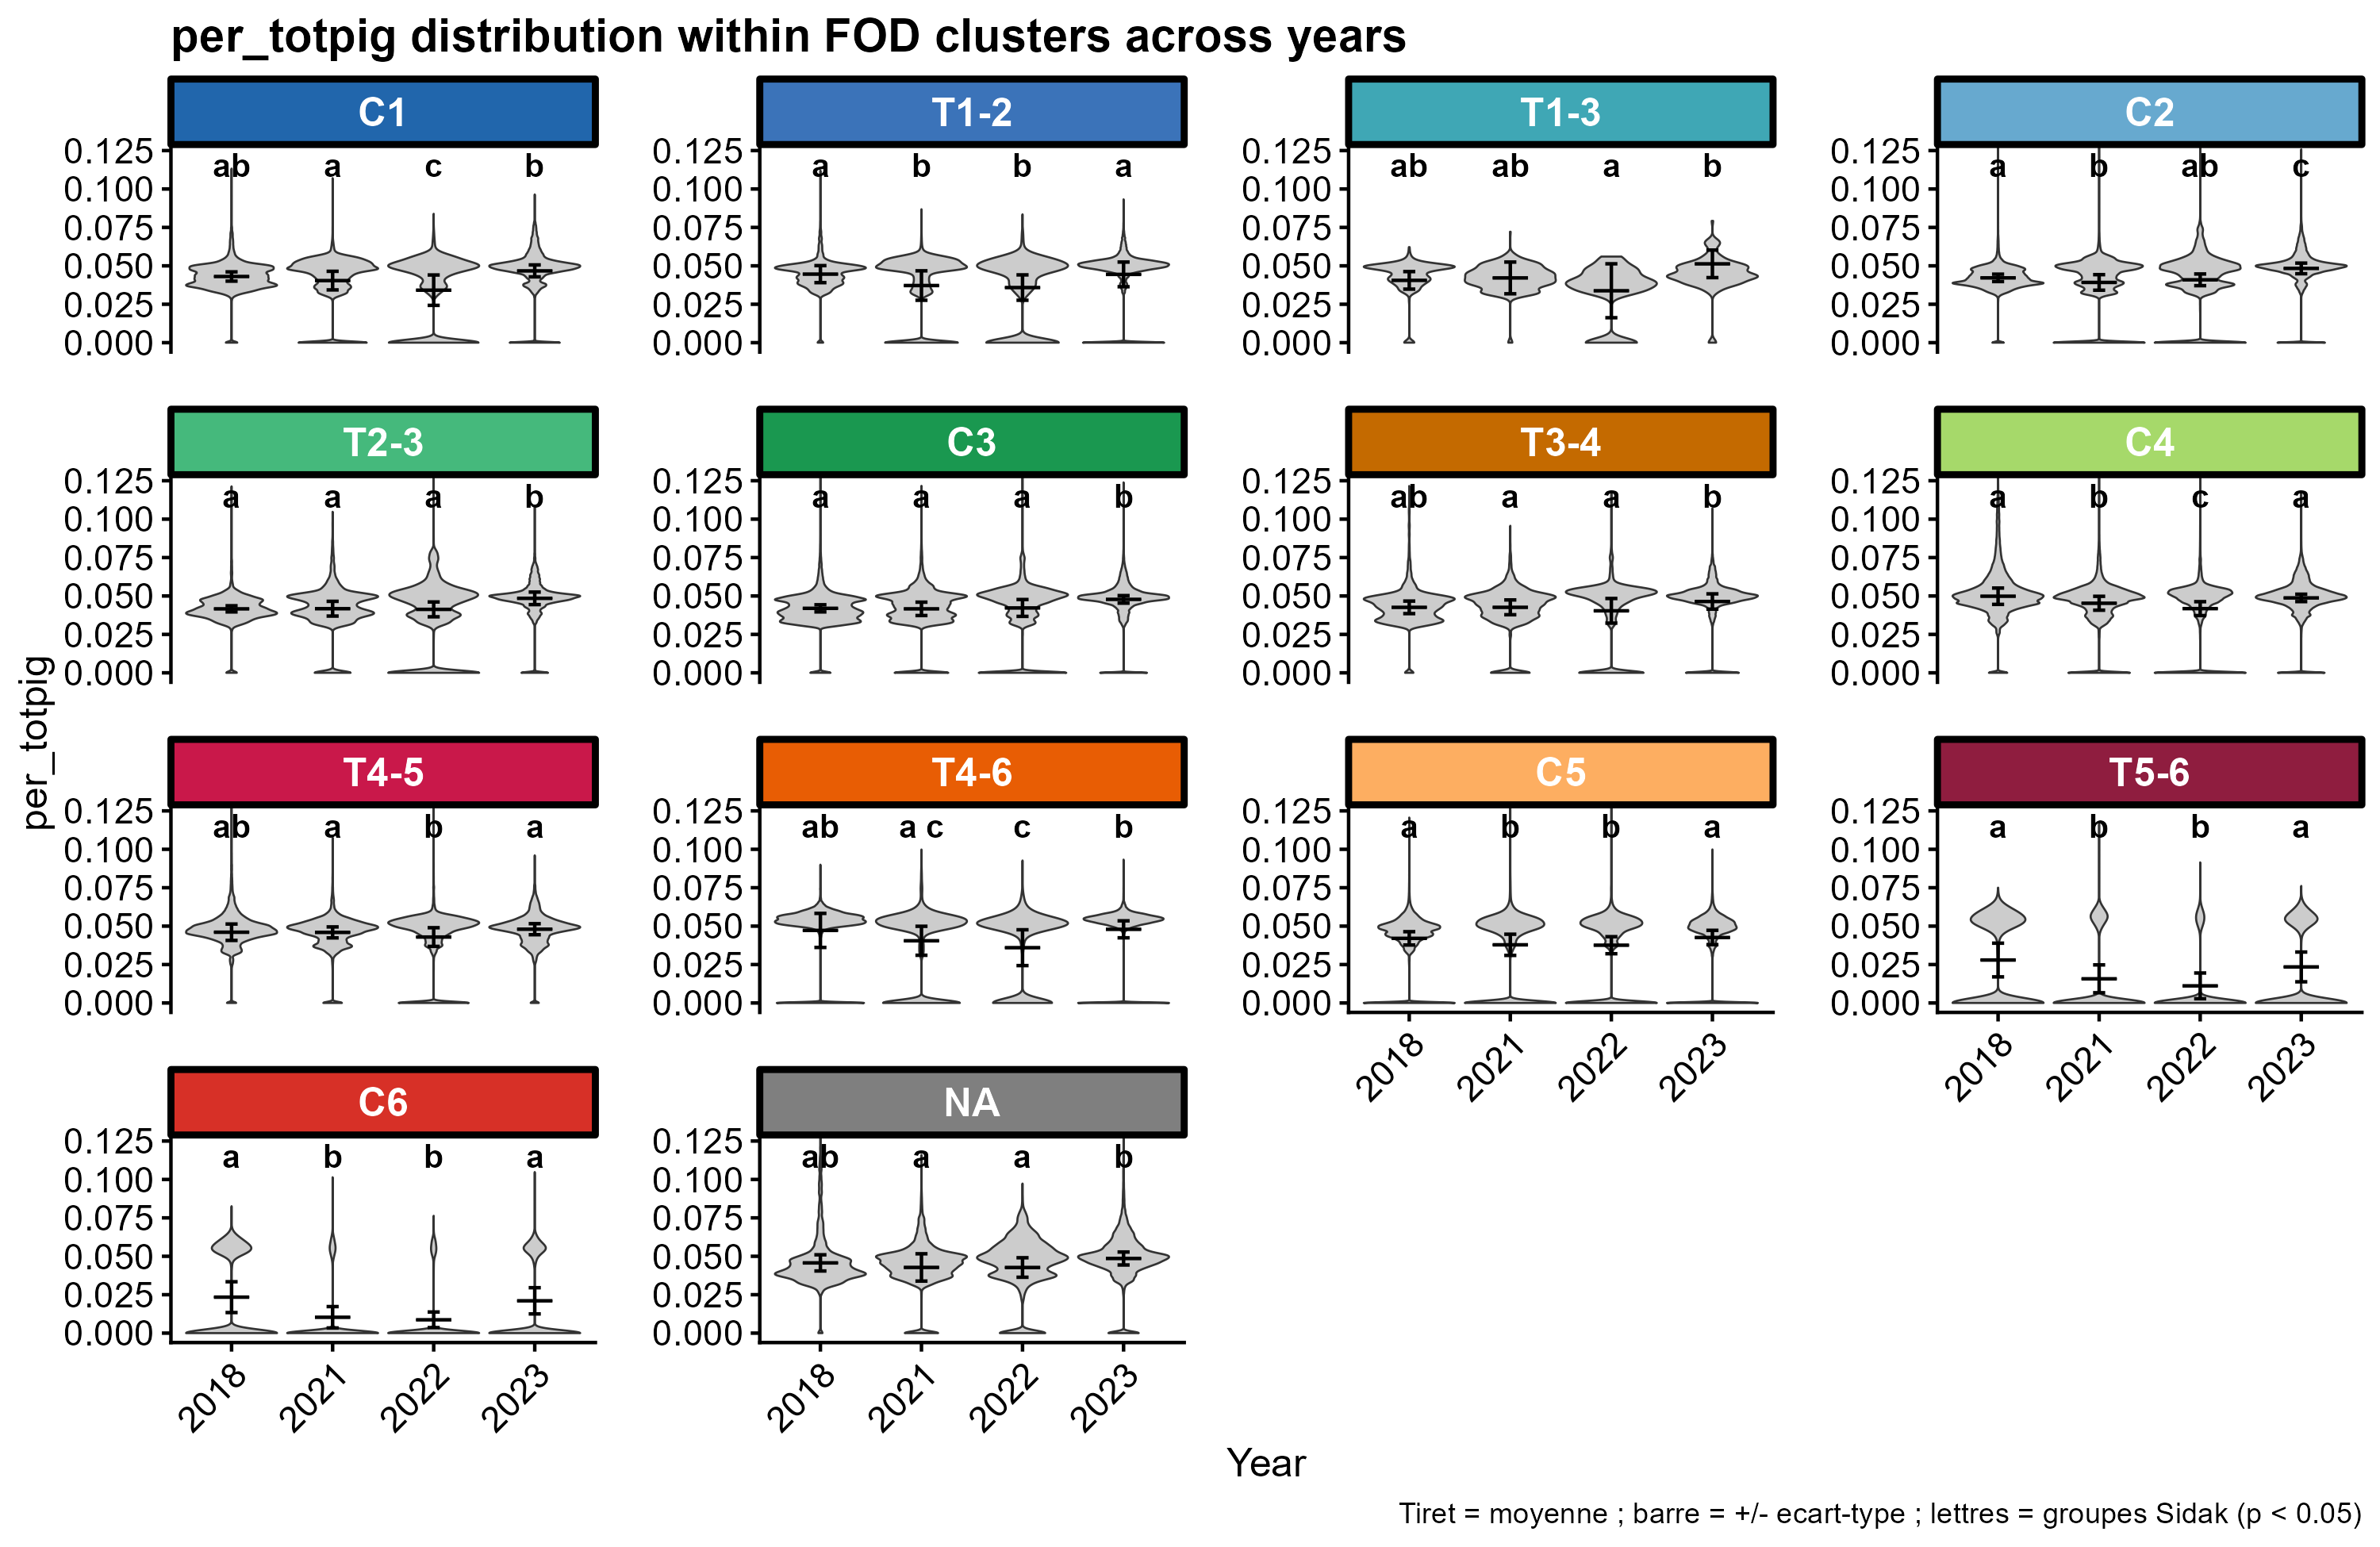
\includegraphics[width=\textwidth]{images/05_annexes/04_resultats/distrib_ftle_nasc_pig_per_fod/violin_per_totpig}
				\caption{Péridinine / $\Sigma$pigments}
			\end{subfigure}
			\hfill
			\begin{subfigure}[t]{0.48\textwidth}
				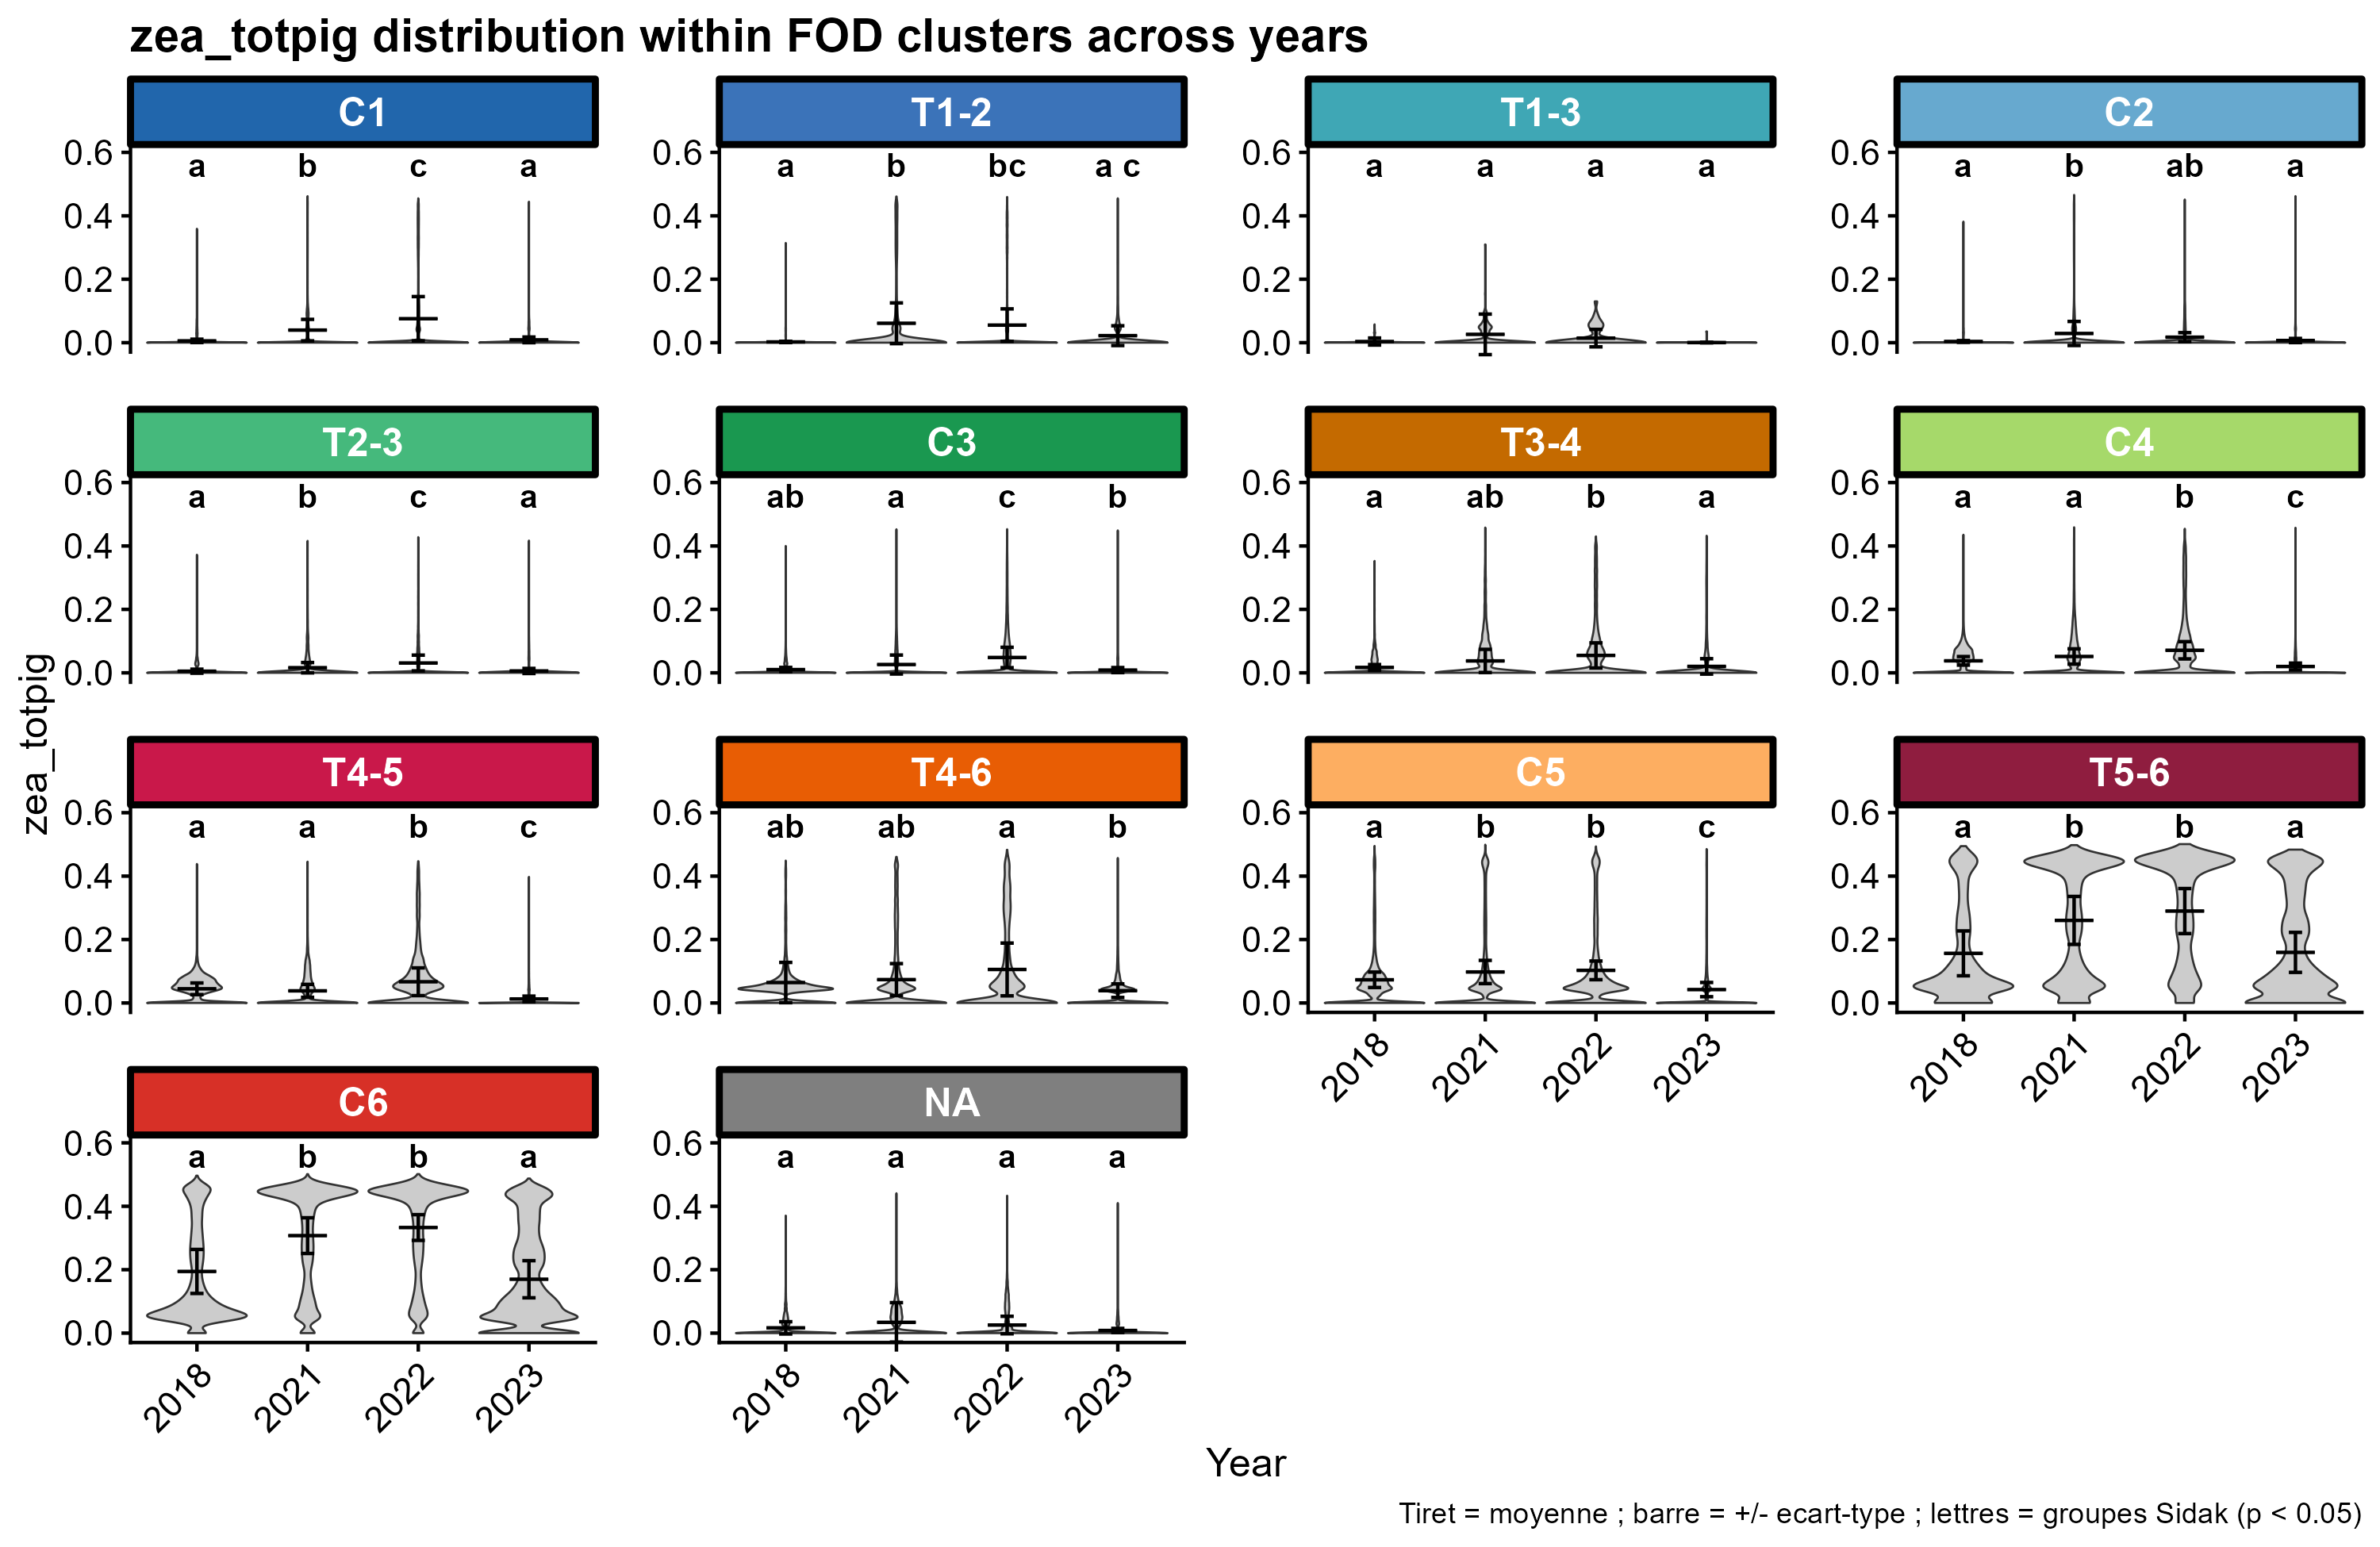
\includegraphics[width=\textwidth]{images/05_annexes/04_resultats/distrib_ftle_nasc_pig_per_fod/violin_zea_totpig}
				\caption{Zéaxanthine / $\Sigma$pigments}
			\end{subfigure}
			
			\vfill
			
			% --- Rangée 2 ---
			\begin{subfigure}[t]{0.48\textwidth}
				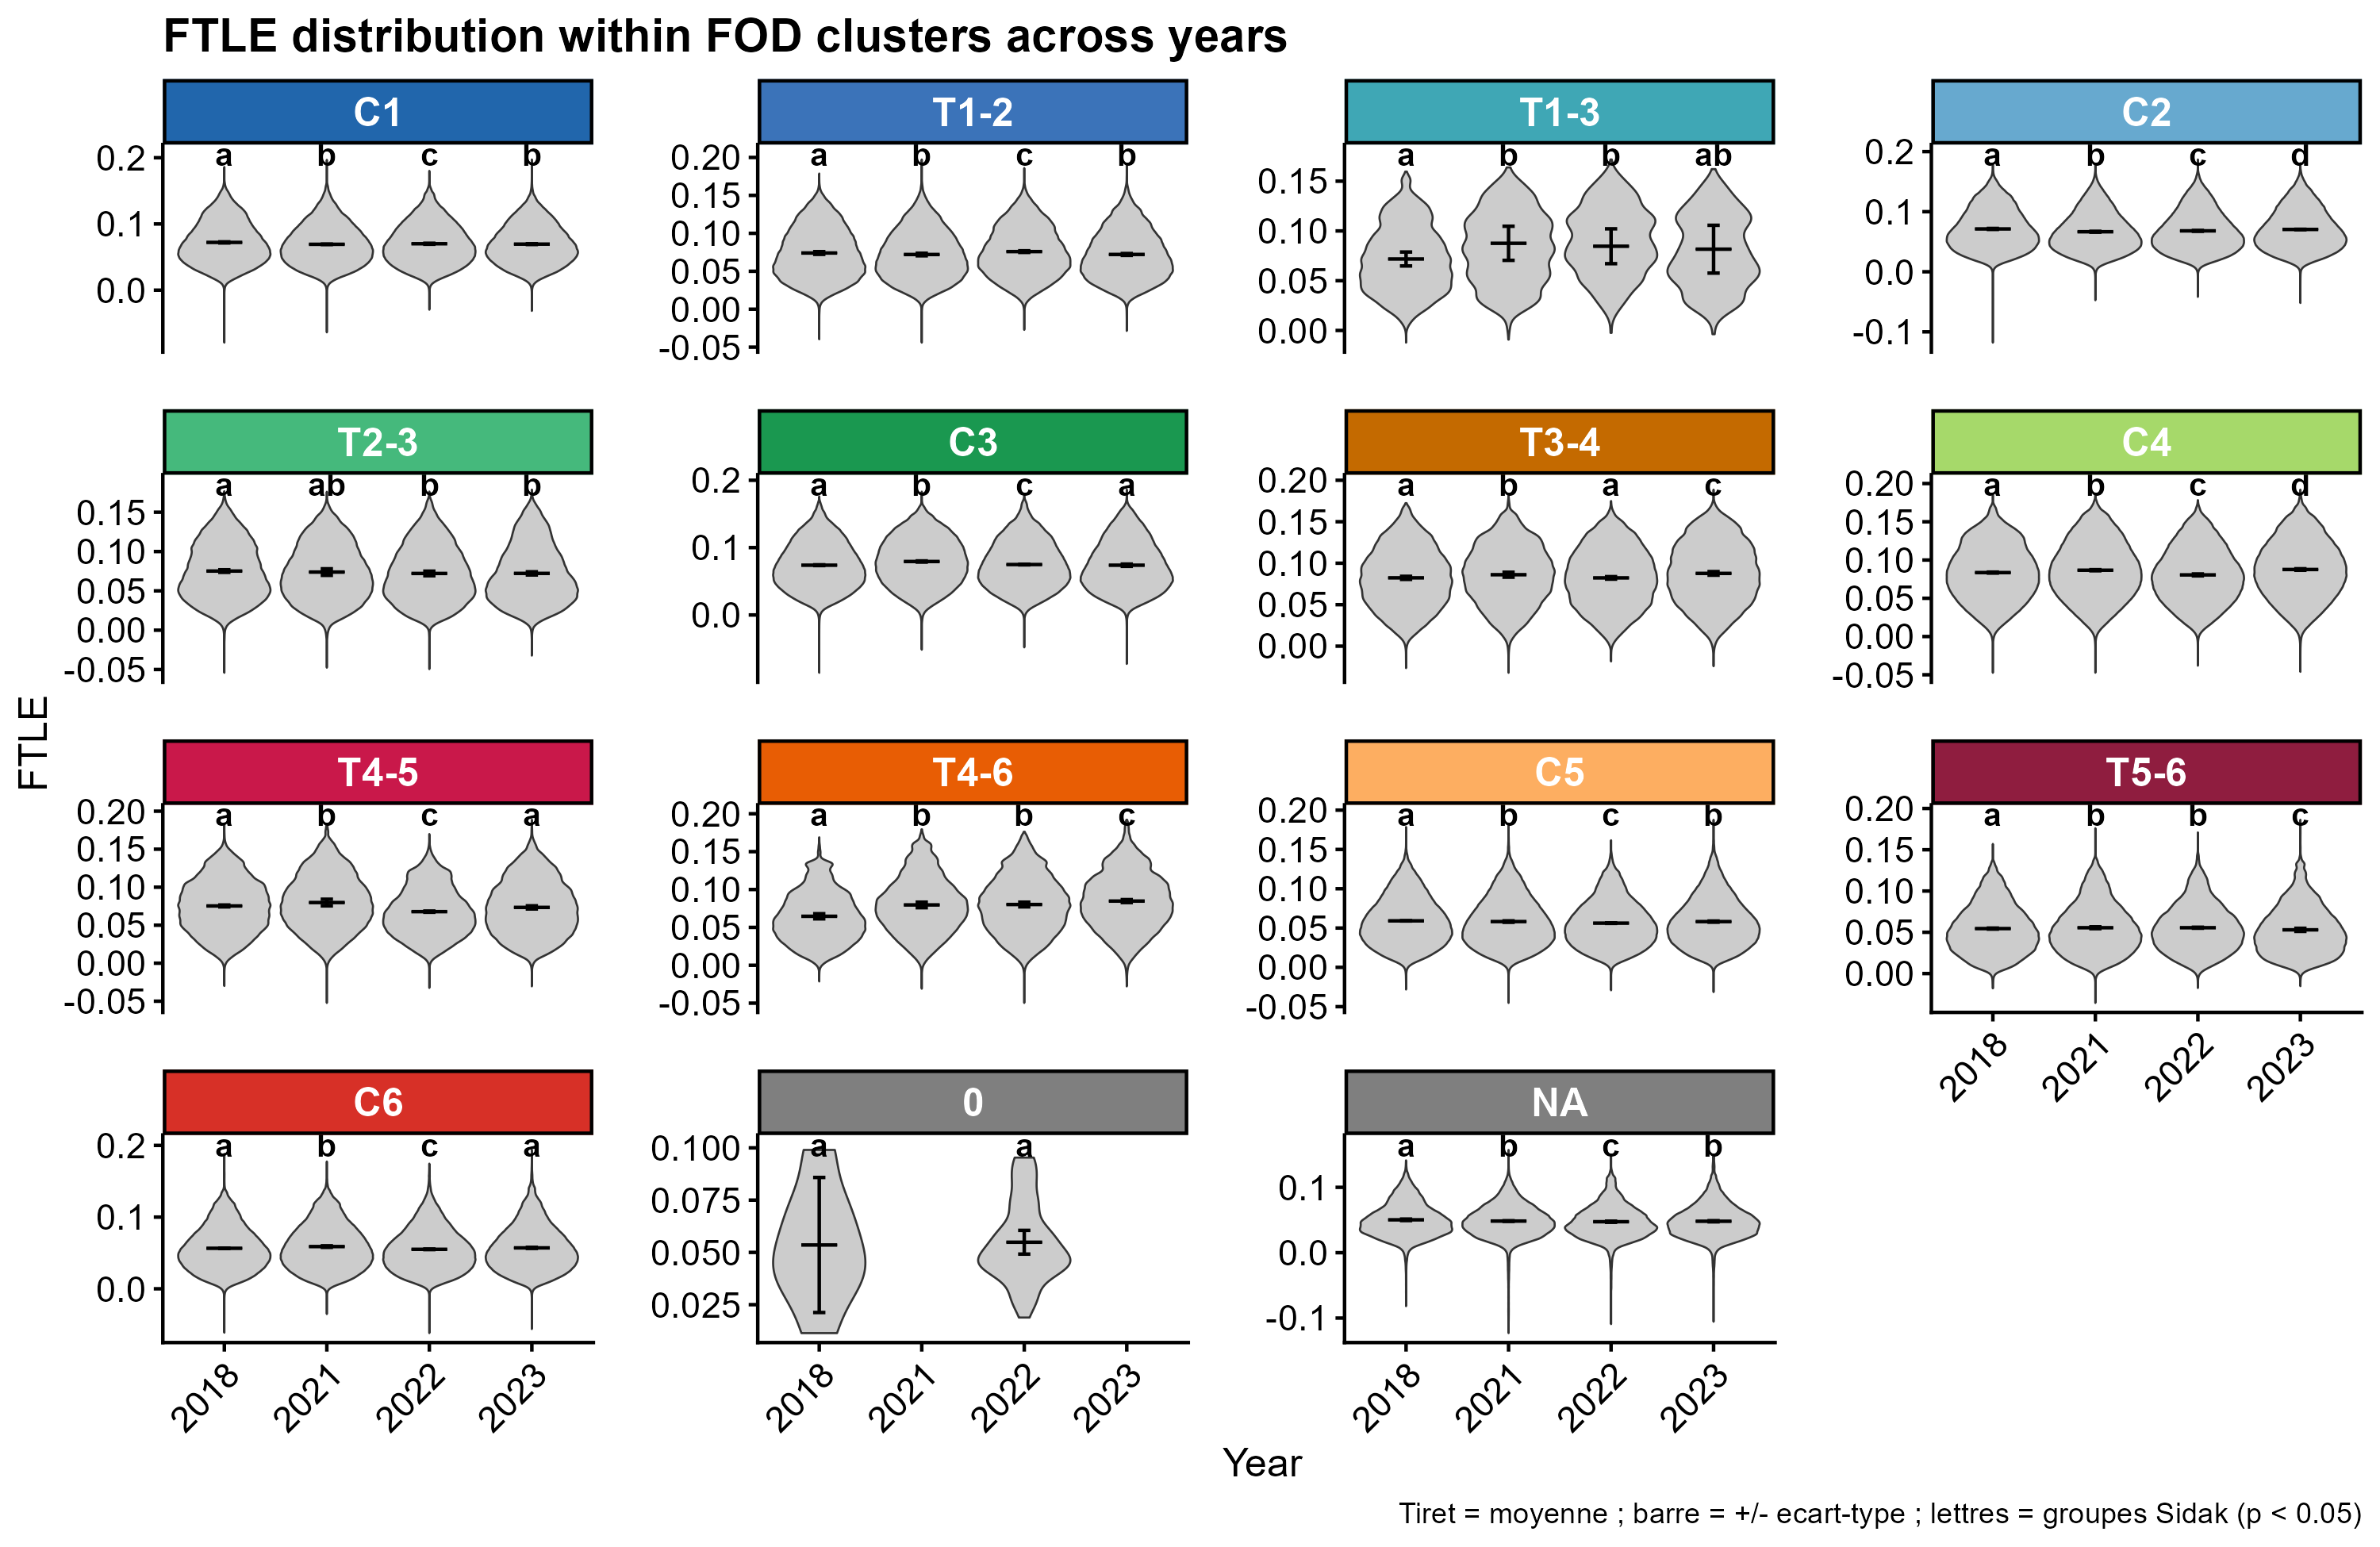
\includegraphics[width=\textwidth]{images/05_annexes/04_resultats/distrib_ftle_nasc_pig_per_fod/violin_FTLE}
				\caption{FTLE}
			\end{subfigure}
			\hfill
			\begin{subfigure}[t]{0.48\textwidth}
				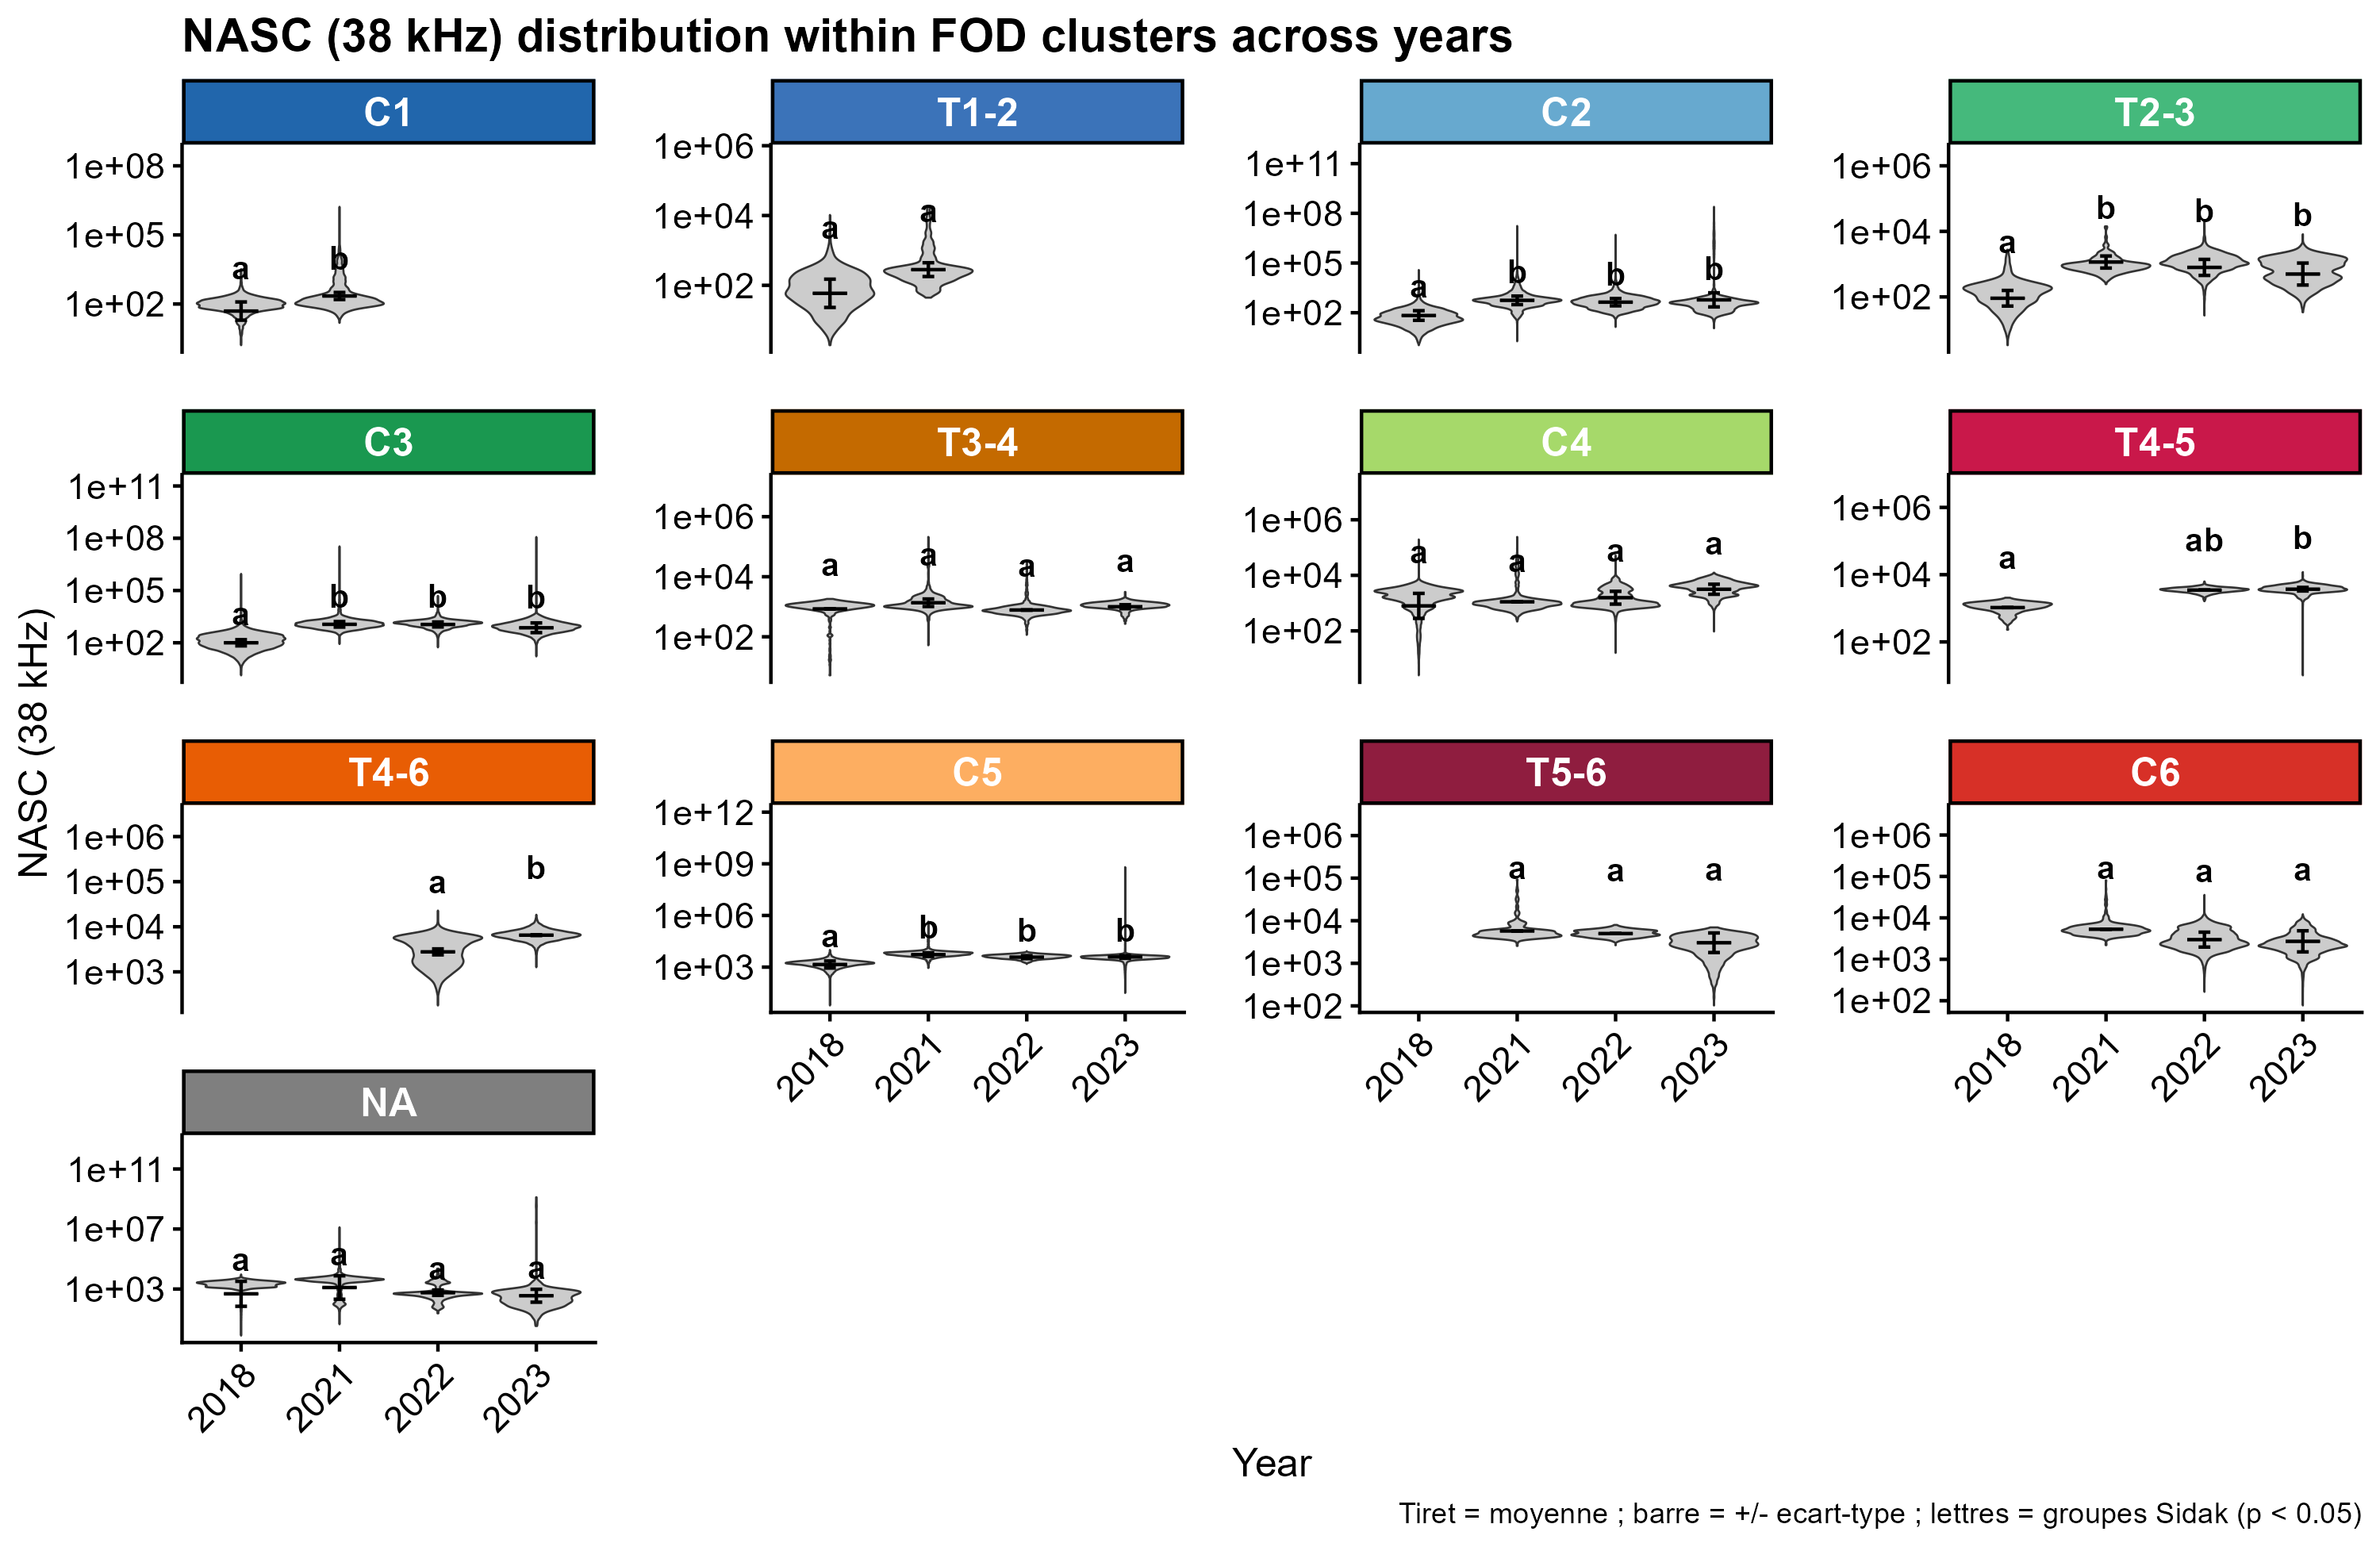
\includegraphics[width=\textwidth]{images/05_annexes/04_resultats/distrib_ftle_nasc_pig_per_fod/violin_NASC__38_kHz_}
				\caption{NASC 38 kHz}
			\end{subfigure}
			
			\vfill
			
			% --- Rangée 3 (1 seule image) ---
			\begin{subfigure}[t]{0.48\textwidth}
				\centering
				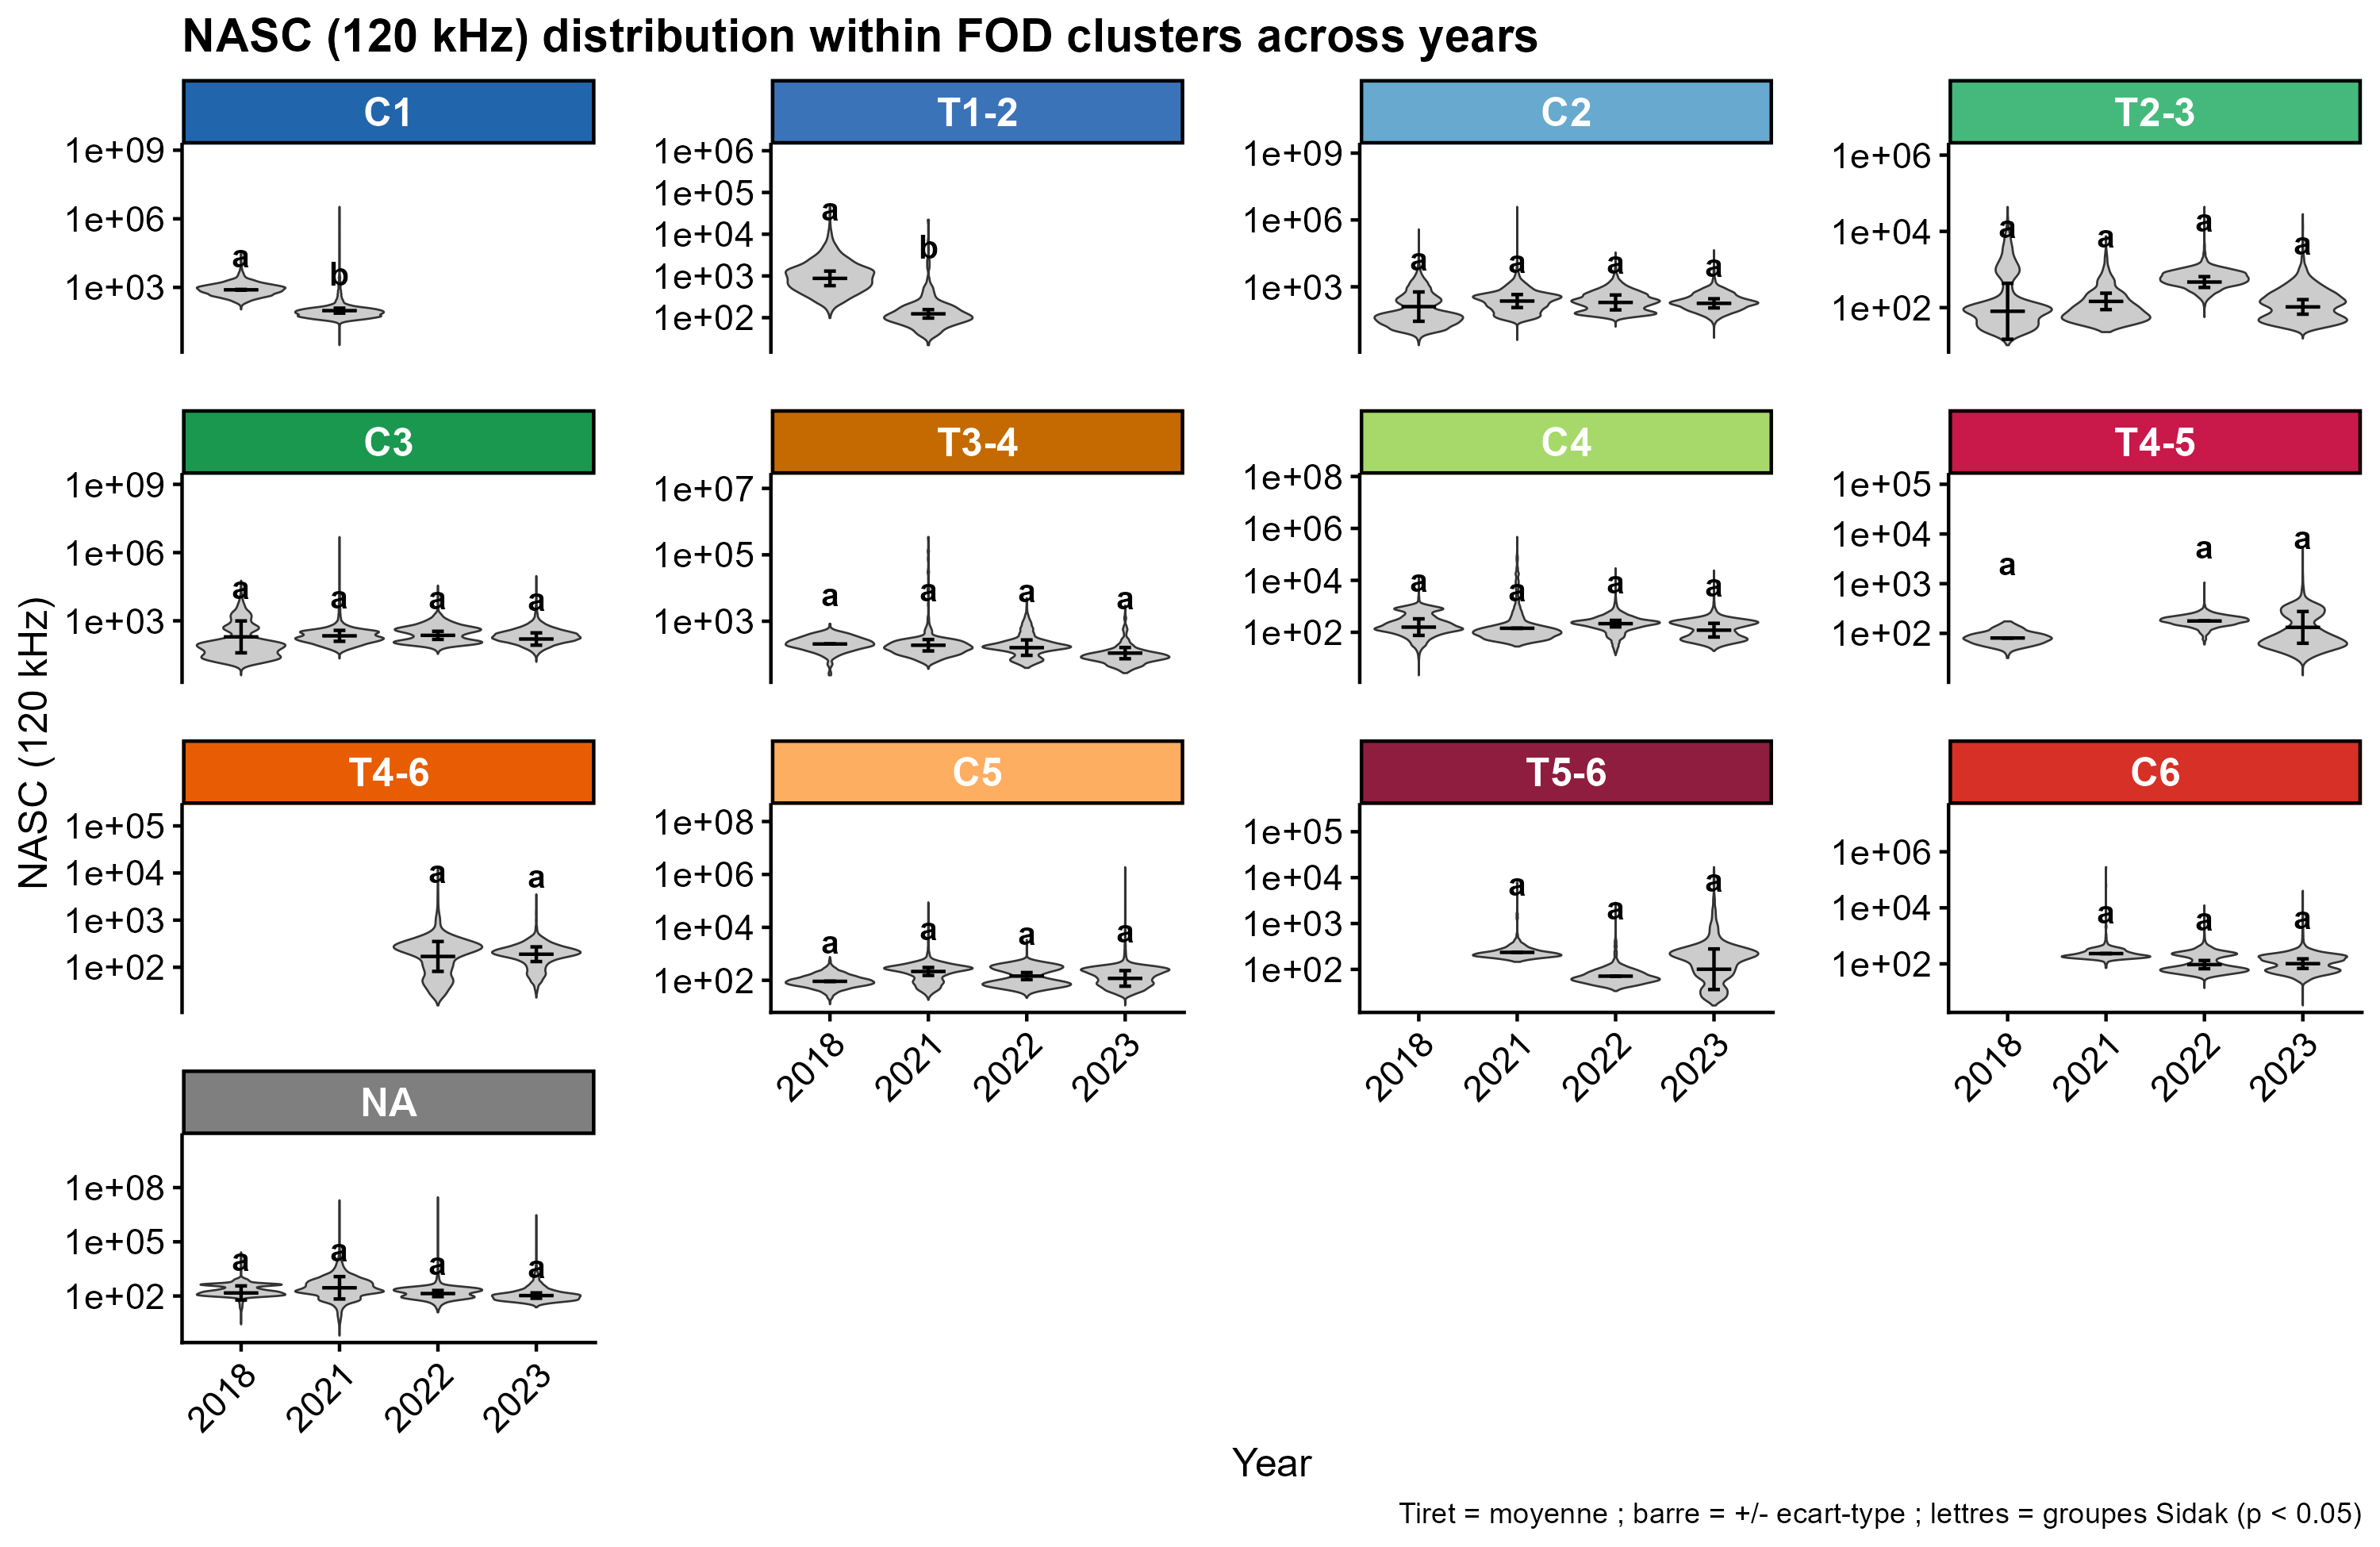
\includegraphics[width=\textwidth]{images/05_annexes/04_resultats/distrib_ftle_nasc_pig_per_fod/violin_NASC__120_kHz_}
				\caption{NASC 120 kHz}
			\end{subfigure}
			
			\caption[Distributions inter-annuelles au sein des clusters FOD]{Distributions inter-annuelles (suite) : variables pigmentaires, FTLE et acoustiques au sein des clusters FOD.}
		\end{figure}
		
	\section{Structure des communautés phytoplanctoniques}
		\label{annexe:distrib_commu_phyto}
		\begin{figure}[H]
			\centering
			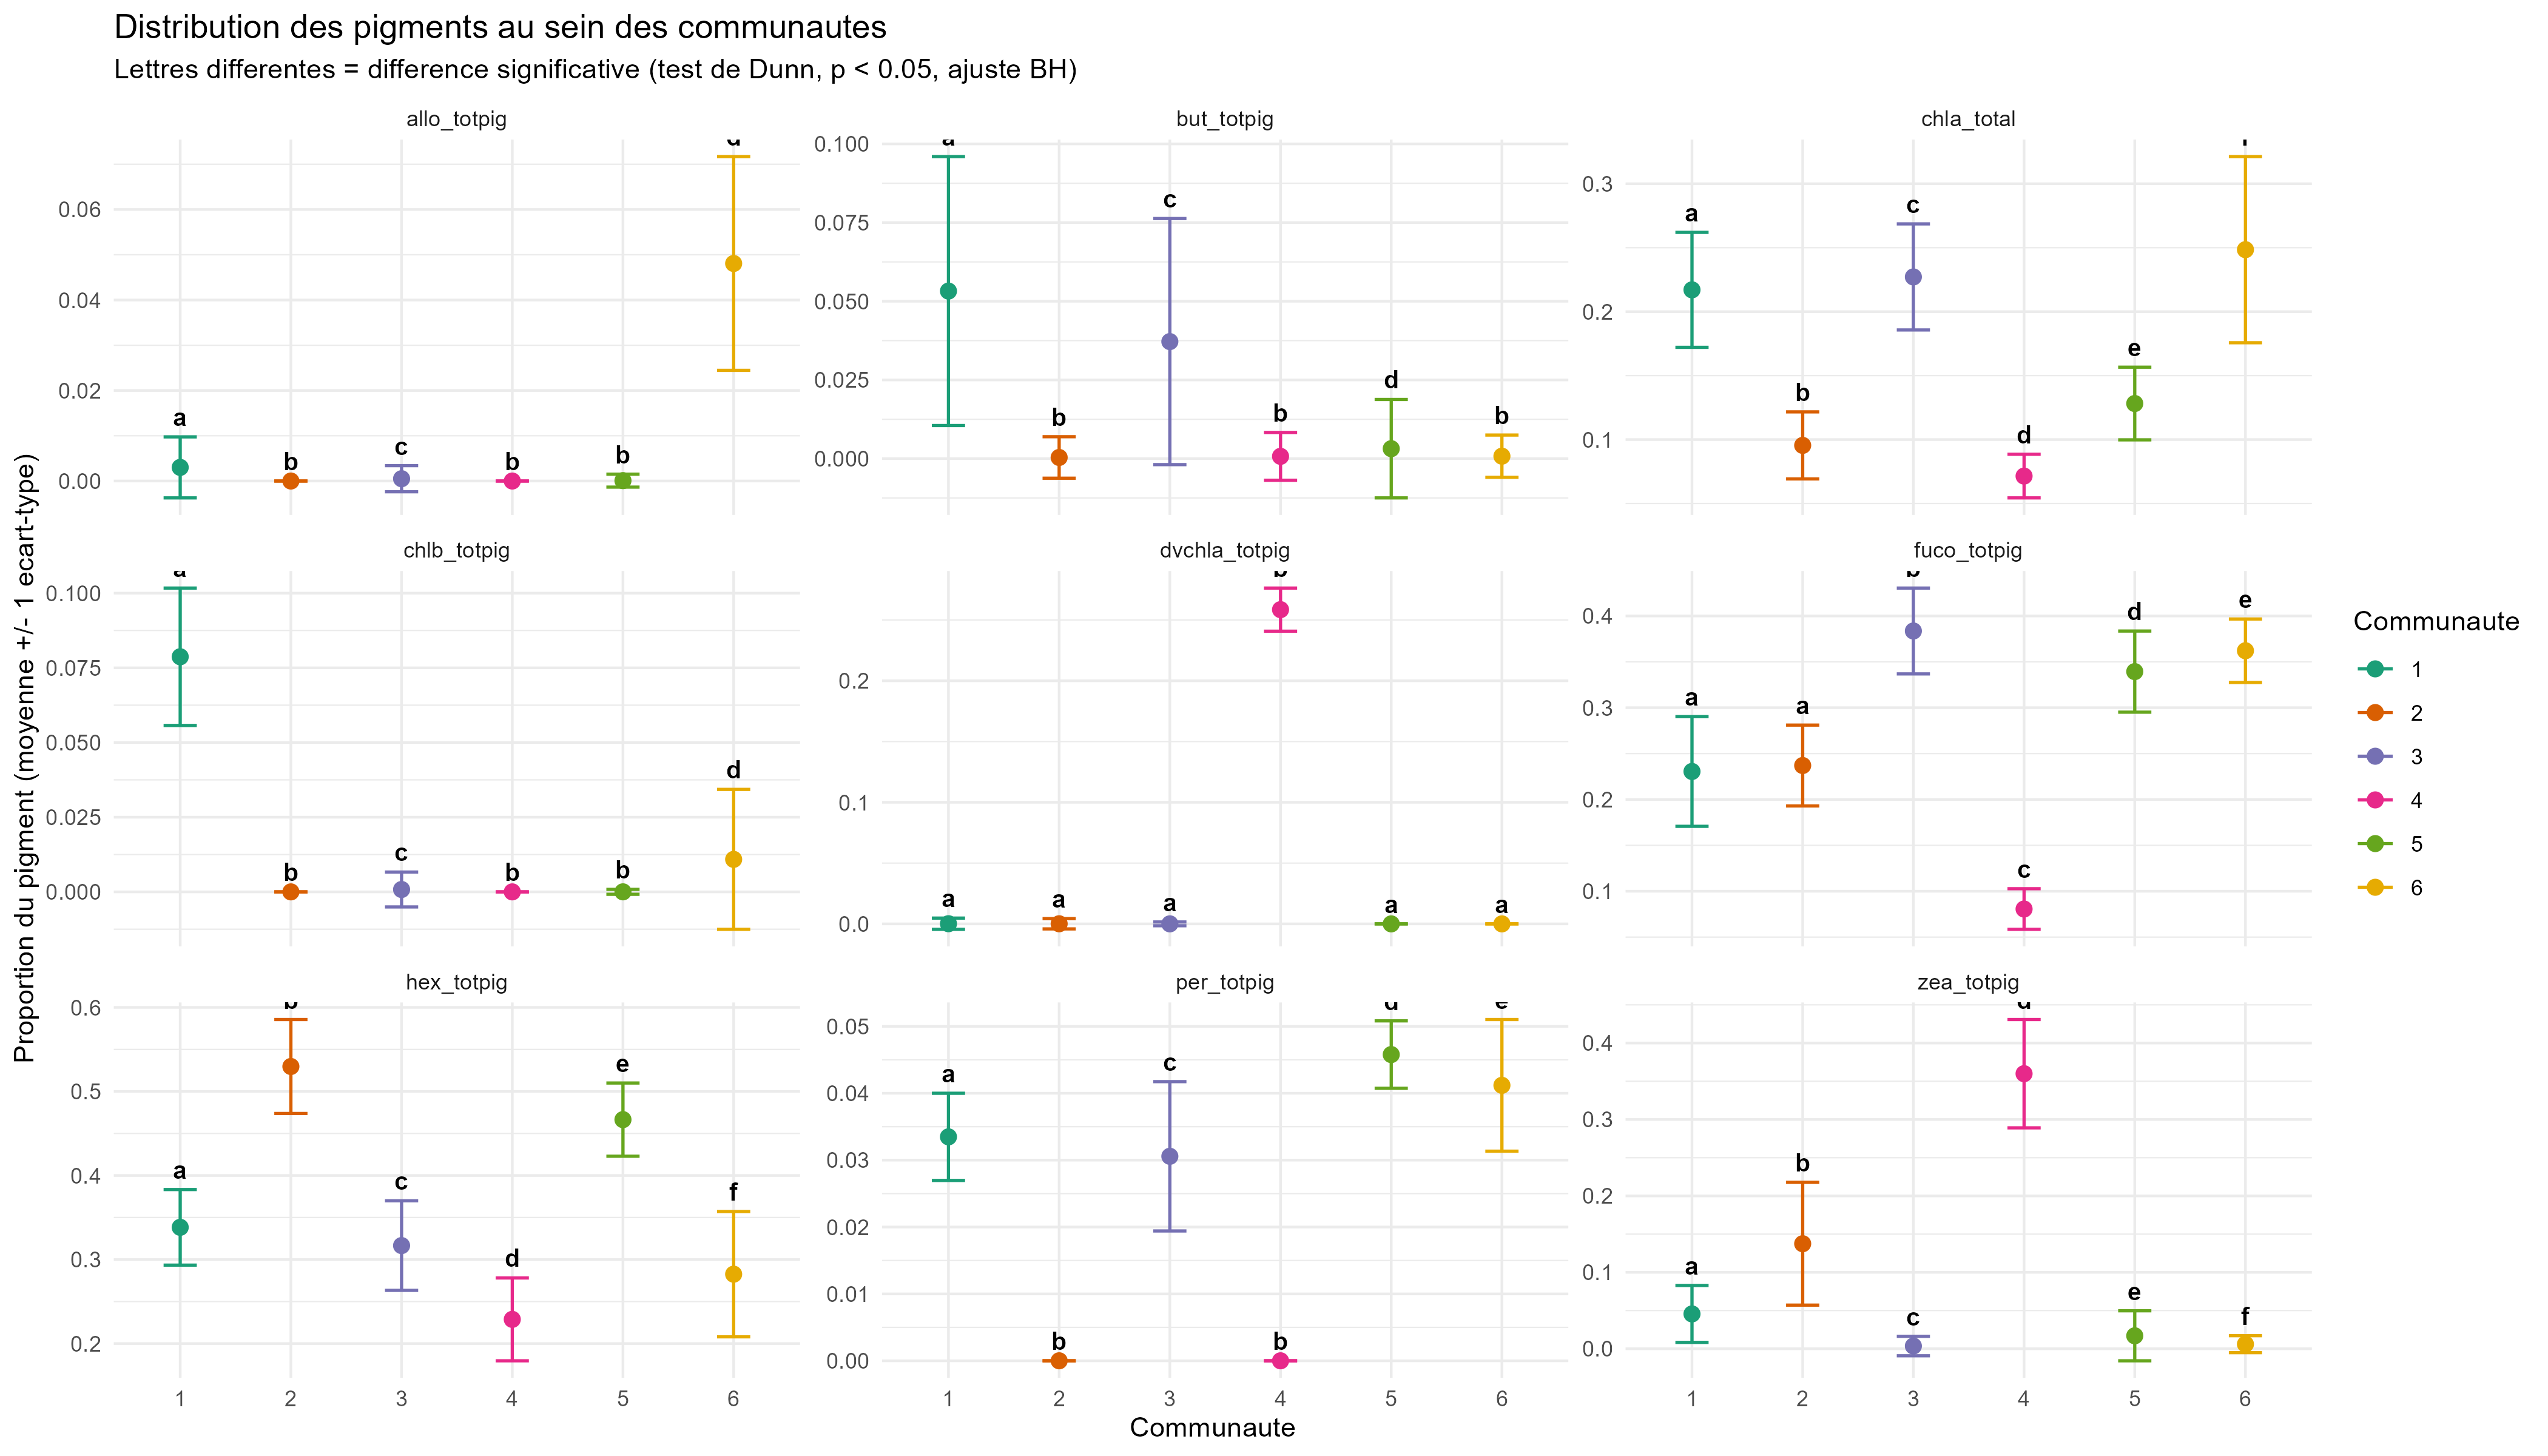
\includegraphics[width=\textwidth]{images/05_annexes/04_resultats/comu_phyto_cluster_pigs/distrib_pigments_in_communautes_kmeans_k6_PFT_stats}
			\caption{Distribution des contribution de pigments par communauté phytoplanctonique.}
			\label{fig:distribpigmentsincommunauteskmeansk6pftstats}
		\end{figure}
		
	\section{Structure prédictive du NASC avec les FOD, FTLE et contributions de pigments}
		- obs vs. preds hist
		- RMSE/R² par fold
		- distance par fold
		- carte du fold 
		- noise robustness
		
	\section{Liens structurels entre le NASC, FOD, FTLE et contributions de pigments}
		- residuals vs latitude
		
	\section{Cartographie du NASC prédit}
		- correlation entre les plots
		- carte de différences
		- Une date de prédiction multidate
		
	\clearpage
	\chapter*{Liste d'abbréviations}
	lon : Longitude
	lat : Latitude
	PSC : Phytoplankton Size Class (Classe de Taille du Phytoplancton)
	PFT : Phytoplankton Functional Type (Type fonctionel de Phytoplancton)
	NASC : Nautical Area Scattering Coefficient (Coeffient de rétropropagation d'aire Nautique)
	ROI : Region Of Interest (Région d'intérêt)
	ESU : Elementary Sampling Unit (unité élémentaire d'échantillonnage)
	\clearpage
	\chapter*{Liste de symboles}
	\clearpage
	\chapter*{Liste des figures et tableaux}
	
	\clearpage
	\chapter*{}
	\printbibliography
\end{document}